





 
\chapter{State of the art}


\section{Inleiding}
 

\section{State of the art}
 
 


\subsubsection{Artificial intelligence en water locks}
   

\section{automatisering van waterwerken}


\subsection{waterwerken}
\subsubsection{Zoekresultaten}
https://hbo-kennisbank.nl/searchresult?q=sluizen 
artificial inte;lligence and water locks 
https://www.sciencedirect.com/science/article/pii/S0160791X21002165 
https://www.wwdmag.com/artificial-intelligence/sewer-monitoring-turns-ai 
https://www.anylogic.com/resources/articles/analysis-of-the-expansion-of-the-panama-canal-using-simulation-modeling-and-artificial-intelligence/ 
ai used in public infrastructure thesis 
https://blog.ferrovial.com/en/2020/10/how-artificial-intelligence-is-used-for-infrastructure-maintenance/ 
https://www.tilburguniversity.edu/about/schools/law/departments/plg/ai-public-sector 
artificaial used in water shipping 
artificial used in maritime transport 
artificaial used in water shipping 
ai used in maritime traffic 



https://www.ftm.nl/artikelen/waternet-verantwoordelijkheid-digitaal-wanbeleid 
https://open.overheid.nl/repository/ronl-bc28f344-af87-481a-aea6-58c481b4cdc8/1/pdf/ilt-onderzoeksrapport-stichting-waternet.pdf\ 
https://www.security.nl/posting/697815/Waternet+onder+verscherpt+toezicht+wegens+onvoldoende+grip+op+cybersecurity 
https://www.security.nl/posting/677368/Inspectie+doet+onderzoek+naar+Waternet+na+verzwegen+penetratietest 
https://www.parool.nl/nederland/onderzoeksraad-rijk-houdt-informatie-over-cyberveiligheid-achter-met-grote-risico-s~b673ec1f/?referrer=https%3A%2F%2Fwww.google.com%2F 


google: artiifcial intelligence for industrial control systems researchgate 
https://link.springer.com/chapter/10.1007/978-3-030-38557-6_7 
automation  for industrial control systems 
researchgate 
google scholar:automation of industrial control systems problems 
hindawi.com: problems industrial control systems    


\subsubsection{bijlmerramp}
Motor 3 (de binnenste motor aan de rechtervleugel van het vliegtuig) brak af, beschadigde de vleugelkleppen en botste tegen motor 4 die vervolgens ook afbrak.
De ernst van de situatie werd op Schiphol niet goed ingezien. Dit kwam onder meer doordat lost in de luchtvaart de gebruikelijke term is om het verlies van motorvermogen te melden. Op Schiphol werd er dan ook van uitgegaan dat er twee motoren waren uitgevallen. Dat ze letterlijk verloren waren wist men niet. Gezien het grote aantal handelingen dat de bemanning in een paar minuten moest uitvoeren en de keuzes die de piloot maakte, veronderstelde de parlementaire enquêtecommissie die de ramp later zou onderzoeken dat ook de bemanning waarschijnlijk niet heeft geweten dat beide motoren van de rechtervleugel waren afgebroken. De buitenste motor van een 747 is vanuit de cockpit slechts met moeite zichtbaar en de binnenste motor helemaal niet.

Op de avond van de 4e oktober 1992 was landingsbaan 06 (de Kaagbaan) in gebruik. De piloot verzocht de luchtverkeersleiding op Schiphol echter een noodlanding te mogen maken op de Buitenveldertbaan (baan 27). Waarom hij juist deze baan koos, is nooit duidelijk geworden. Een keuze voor deze baan lag niet voor de hand; omdat de wind uit het noordoosten kwam, zou het toestel met flinke staartwind moeten landen. Langs de landingsbaan waren enkele grote brandweerwagens van Schiphol geplaatst. Deze zogeheten crashtenders moesten een brand tijdens de landing meteen blussen. Na de crash werd één zwarte doos teruggevonden. De bijbehorende band was in vier stukken gebroken, waardoor de laatste 2 minuten en 45 seconden ervan niet meer te gebruiken waren. De doos werd voor onderzoek naar Washington gestuurd en leverde uiteindelijk onderstaande informatie op.
Om goed uit te komen voor de landingsbaan vloog het beschadigde toestel eerst nog een rondje boven Amsterdam. Tijdens dit rondje gaf de gezagvoerder de copiloot opdracht de vleugelkleppen (flaps) uit te schuiven. Links schoven de kleppen uit, maar doordat de afgebroken motor 3 de rechtervleugel had beschadigd schoven de kleppen op die vleugel niet uit. Als gevolg hiervan kreeg het toestel links meer draagvermogen dan rechts. De piloot meldde aan de verkeersleiding dat er ook problemen met de flaps waren.
Aanvankelijk ging het aanvliegen van de Buitenveldertbaan goed. Op het moment dat het vliegtuig daalde tot onder de 1500 voet en snelheid minderde, raakte het echter compleet onbestuurbaar en maakte het een ongecontroleerde, scherpe bocht naar rechts. Over de radio was te horen dat de gezagvoerder zijn copiloot in het Hebreeuws opdracht gaf om alle kleppen in te trekken en het landingsgestel uit te klappen. Vervolgens meldde de copiloot in het Engels aan de luchtverkeersleider dat het toestel zou gaan neerstorten. Uit later onderzoek bleek dat het vliegtuig eerder enkel recht bleef vanwege de hoge snelheid (280 knopen, zijnde 519 km/u). Doordat de rechtervleugel beschadigd was, was het moeilijker om het vliegtuig recht te houden. Alleen de hoge snelheid zorgde ervoor dat er nog voldoende draagvermogen was. Toen bij het inzetten van de landing de snelheid verlaagd werd, werd het draagvermogen van de rechtervleugel echter dusdanig gering dat het toestel niet meer onder controle te houden was en een duikvlucht naar rechts maakte.

https://aviation-safety.net/database/record.php?id=19921004-2&lang=nl    
\input{cyber aanval op Oekraïene}   

\section{ecourt in nederlandse rechtspraak}
niet odnerzocht   




\subsection{ethiek}


Ethiek 



persuasive technology 
https://www.humanetech.com/youth/persuasive-technology 
https://www.minddistrict.com/blog/persuasive-technology-new-insights-in-behavioural-change 
https://www.sciencedirect.com/book/9781558606432/persuasive-technology 
https://spectrum.ieee.org/how-persuasive-technology-can-change-your-habits 
https://www.frontiersin.org/articles/10.3389/frai.2020.00007/full 
https://psmag.com/environment/captology-fogg-invisible-manipulative-power-persuasive-technology-81301 
https://www.makeuseof.com/what-is-persuasive-technology/ 
https://lib.ugent.be/catalog/rug01:001235489 
https://cyberpsychology.eu/article/view/12270 
   


\subsubsection{ethiopian airlines}
Ethiopian Airlines Flight 302
Door problemen met de flight control
One minute into the flight, the first officer, acting on the instructions of the captain, reported a "flight control" problem to the control tower.
Two minutes into the flight, the plane's MCAS system activated, pitching the plane into a dive toward the ground. The pilots struggled to control it and managed to prevent the nose from diving further, but the plane continued to lose altitude.
The MCAS then activated again, dropping the nose even further down. The pilots then flipped a pair of switches to disable the electrical trim tab system, which also disabled the MCAS software. However, in shutting off the electrical trim system, they also shut off their ability to trim the stabilizer into a neutral position with the electrical switch located on their yokes. The only other possible way to move the stabilizer would be by cranking the wheel by hand, but because the stabilizer was located opposite to the elevator, strong aerodynamic forces were pushing on it.
As the pilots had inadvertently left the engines on full takeoff power, which caused the plane to accelerate at high speed, there was further pressure on the stabilizer. The pilots' attempts to manually crank the stabilizer back into position failed.
Three minutes into the flight, with the aircraft continuing to lose altitude and accelerating beyond its safety limits, the captain instructed the first officer to request permission from air traffic control to return to the airport. Permission was granted, and the air traffic controllers diverted other approaching flights. Following instructions from air traffic control, they turned the aircraft to the east, and it rolled to the right. The right wing came to point down as the turn steepened.
At 8:43, having struggled to keep the plane's nose from diving further by manually pulling the yoke, the captain asked the first officer to help him, and turned the electrical trim tab system back on in the hope that it would allow him to put the stabilizer back into neutral trim. However, in turning the trim system back on, he also reactivated the MCAS system, which pushed the nose further down. The captain and first officer attempted to raise the nose by manually pulling their yokes, but the aircraft continued to plunge toward the ground.

https://www.hindawi.com/journals/ijae/2014/472395/    



\subsubsection{explosie in libabon, beirut 
}

Op 23 september 2013 voer het vrachtschip de Rhosus onder Moldavische vlag[7] van Batoemi in Georgië naar Beira in Mozambique met 2.750 ton ammoniumnitraat

Gezien het ernstige gevaar van het bewaren van deze goederen in de hangar onder ongeschikte klimatologische omstandigheden, herhalen we ons verzoek aan de marine-instantie om deze goederen onmiddellijk weer te exporteren om de veiligheid van de haven en de mensen die er werken te verzekeren, of om akkoord te gaan om ze te verkopen.
Voorafgaand aan de explosie was er een brand in een opslagplaats. 

https://www.hrw.org/report/2021/08/03/they-killed-us-inside/investigation-august-4-beirut-blast 
https://www.researchgate.net/publication/348325979_Beirut_Explosion_the_full_story 
https://reliefweb.int/sites/reliefweb.int/files/resources/CaseStudy_BeirutExplosion_TechBioHazardsweb.pdf    
\input{explosie tanjin china }   
\newpage

\section{Literatuuronderzoek}





\subsection{Introductie}




Een definitie of omschrijving van het onderwerp in brede termen, of van de issues die je wilt onderzoeken, dit geeft de lezer context waarin de literatuur wordt onderzocht of bekenn. De belangrijkste trends in deze sector van de literatuur, de algemene theorien en de gebieden waarover wordt gediscussierd, en mogelijk gaten in de literatuur.
Een verklaring waarom je deze literatuur reviw uitvoert en het standpunt dat je zal innemen bij het uitvoeren van een kritische analyse.
De manier waarop de reviw wordt gepresenterd.
Een verklaring  van waarom bepaalde literatuur niet wordt meegenomen in de studie.
\subsection{Middenstuk}



Begin emt een discussie van de algemene modellen en theorien, die passen bij deze studie. Groepeer belagrijke themas of trends en bediscussier deze in detail. Begin algemeen en ga veervolgens in op specifiekke details, dit geldt voor het gehele literatuur review en de individuele onderdelen.
Probeer te verklaren, en indien nodig, tegenstrijdigheden  op te lossen in wat je rapporteert. Neem alle onderwerpen over die relevant zijn voor de dissertatie.
Pak breedt uit om te zorgen voor een solide grondslag, zodat er een basis/ondersteuning is voor de slot van de dissertatie.
Conclusie


Aan het einde van de literatuur review, in deze conclusie, moet je expliciet duidelijk aken wat de research objectives zijn  van het onderzoek, zo dat de lezer niet twijfelt over wat je wilt onderzoeken.
Om dit te bewerkstelligen moet je:
Een opsomming geven van de belangrijke punten die door het literatuuronderzoek worden meegenomen.
Geef een overzicht vand e gaten in de literatuur, als deze er al zijn, en gebruik deze mo aan te geven waarom dit onderzoek belangrijk/relevant is.
Remember  that  your  literature  review  should  lead  and  justify  the research objectives and questions of your dissertation.




\subsection{Literatuur review}



Presenteren en analysern van, op een kritische manier, dat gedeelte van de gepubliceerde literatuur dat relevant is voor jhou onderzoeksonderwerp en dat als grondslag kan funderen voor het beter begrijpen van de context waarini je onderzoek uitvoert, en dus de lezer te helpen  eeen beter beeld te krijgen van wat je hebt gedaan,
Kritisch zijn betekent niet alleen naar de negatieve kanten kijken maar om te evaluereren.
Om als chtergrond te dienen voor wat je hebt gedaan in het slot van je onderzoek mag worden geanaluseerd en kritisch worden geevalueerd zodat de lezer de kans krijft toegang te krijgen tot jou schijfvaardigheden, analystische vermogen en onderzoekssvaardigheden.
OM aan te tonen dat jet niet alleen ontdekt engerapperteerd hebt wat je relevant vind in literatuuronderzoek, maar dat je het hebt begrepen en dat je in staat bent het te analyseren opp een kritische manier.


OM aan te tonen dat jou kennis van het onderzoeksdomein gedetailleerd genoef if om gaten te vinden in bestaande kennis over het onderwerp; wat als reden fungeert voor jouw onderzoek. Om aan te tonen dat jij de sleutelvariabelen jend, trends en actoren in de omgeving van je studie, ie om aan te tonen dat je weet wat belangrijke omderwerpen zijn  die moeten worden onderzocht.
OM de lezers in staat te stellen de geldigheid van je keuze voor een onderzoeksmethode te beoordelen, de toepasselijkheid van het process waarmee je resultaatten analyseert en of je bevindingen congruent zijn met eerdere onderzoeken.


Het literatuuronderzoek is gepresenteerd in de vorm van een precis, een classidficatie, een vergelijking van een kritische analyse van het materiaal dat gelijk is aan een volledige begrip van ou onderzoeksstudie. Zulk gepubliceerd materiaa mag van overl vandaan gehaald worden: een combinatie van tekstboeken, wetenschappelijke artiekelen, conferentie verslagen, rapporten, case studied, het internet, tijdschriften of nieuwsartiekelen. Belangrijk is niet te vergeten dat de meest belangrijke academische literatuurartiekelen de wetenschappelijke artikelen zijn en dat je er zeker van moet zijn dat je bekent bent met de meest recente publicaties die bekent zijn in je onderzoeksveld.
Wees ervan bewust dat hou literatuuronderzoek  moet leiden en een rechtvaardighing moet bieden aan research objectives en  vragen van je dissertatie. Joyw literatuur review is niet alleen een catalogus van auteurs, raamwerken en ideen maar moet pogen een kritische evaluatie van deze auteurs te introduceren.
Een literatuur review is ongeveerd tussen 3000 en 4000 woorden



\subsection{Research methodology}






Je begint de research methodologie met het stelen van de onderzoeksdoelen van het project. Dit stelt de lezer in staat te beoordelen of je onderzoeksmethode te valideren is.

Dit hooffdstuk is het deel van de dissertatie waar je de kant hebt om de lezer te overtuigen dat het proces waaruit de onderzoeksvragen uit voortkomen, die afgeleid zijn van een analyse van relevante onderzoeken, worden beantwoord. Hte is niet voldoende te zeggen dat er een acceptabele groep is odnerzocht et behulp van quota sampling tehnieken en dat er vervolgens een observatie is uitgevoerd met een summiere vragenijst. Het kan wel een geval zij  dat gegeven een probleem dat wordt onderzocht, een dergelijke manier van odnerzoeken gerechtvaardigd is. Maar als e niet de kans hebt genomen je onderzoeksje=keuzes te odnerbouwen aan een lezer dan kunnen zij terecht aannmen dat je bij kans hebt aangenomen, of misdschien wel hebt gegokt wat kan werken en wat niet kan werken, en op gelu hebt beoordeeld en toevallig bij het juiste oploing bent gestuit.
De term methodologie  betekent niet alleen methodem maar ook de werkende filosife achter de methode die zijn gebruikt.


Het hoofdstuk over onderzoekmethhode moet een reden opleveren voor elke beslissing die i genomen bij aankomst en de weg waarin het onderzoek is georganiseerd. Elke keer dat hjij als onderzoeker, een keuze moet maken tussen een aantal opties moet  jij kunnen vertellen welke keuze je hebt gemaakt en waarom en warom je andere hebt afgewezen, Dit hoofdstuk is tussen de 100 en 2000 woorden,

\subsection{Findings / Results / Data Analysis}
.





Data
Dit hoofdstuk toont de bewijs en andere onderzoeksreusultaten van primair onderzoek dat je hebt uitgevoerd. Afhankelijk van je onderzoeksgebied kan dit zijn in de vorm van kwantitatieve gedetailleerde modellen,  hypotheses testen tot een andere vorm van bsis analyse of basis descriptief statistiek of kwalitatieve technieken  met gestructureerde content analyse, tekstuele analyse, tot case studie omschrijvingen.

Het hoofd deel van dit hoofdstuk is de presentatie van de taia die he bent verworven. Zelfs projecten met moderne toepassingen zullen een grote hoeveelheid aan data gnreeren die moet worden bekeken, De data moet worden georganiseerd in een logisch coherente manier zodat jouw gedachtegang en interpretatie duidelijk zijn voor de lezer.

Welke vorm van dat nalyse dan ook wordt uitgevoerd, het moet worden volbracht met zorgvuldigheid en oog voor detail, alsook de manier waarop de resultaten worden getoond, Niets is meer fresutrerend voor een leer dan zich een weg te banen in de tabellen, figuren en statistieken. BEter om het in  toegankelijke manier op te schrijven wat het ondezok heeft blootgesteld en alleen te tonen wat pertinetn kan worden getoond als bewijs voor je bevindingen.


Dissertateis die worden bijgeleverd met gedetailllerde modellen of kwantitatieve analysen moeten zekere alle relevante aannames tonen alsook relaties en methoden. Jouw academische supervisor zal in staat moeten zijn om advies te geven over het level van detaul dat nodig is in het middenstuk alsook in de bijlagen.
grafieken, diagrammen, pei-charts zijn allemaa bruikbaar als manier om je onderzoeksresultaten te onen, zijn kunnen vehelderen zijn  integenstelling tot grote blokken tekst en geven meer body aan de inhoud.

Houd je bij jouw review bij de items die relevant zijn voor je onderzoeksvragen en niet alles wat is gevonden.

Er zullen problemen zijnin de uitvoer van elk onderzoek en hun voorkomen moeten duidelijk worden gemaakt aan de leer. zonder deze te benoemen, zal een essentieel element van de context waarin het onderzok plaatsvind ontbreken.


Niet alle dissertatie hebben kwantitatieve data, In veel sitauties, hebben studenten en uitgebreid gebruik van kwalitatieve onderzoekstechnieken zoals focus groups en of ongestruturerde diepte interviews. terwijl kwantitatieve data zelf leidt tot een grafieken, tabellen enzovoorts, kwalitatieve data en de manier waarop het is gepresenteerd, zijn een uitdaging voor studenten.  Zoals altijd moet jouw doel gebaseerd zijn op een overtuiging dat ata moet worden getoond op een dusdange manier dat het makkelijk is voor de lezer om de logica van de analyse te begrijpen.



De analyse van kwalitatieve data moet gebaseerd zijn op een ondrzoeksvraag en issues die je hebt verkend tijdens je veldwerk Bijvoorbeeld, je hebet zes of zeven kritiesche vragen over een reekrs artiekeln Elk van deze vragen zou op zich moeten worden bestudeerd, in plaats van ze te beschrijven voor elke focus groep, Dit verschaft een logische flow en ontwikkeling in de analyse
Daarbij, it het aannemelijk te focussen op punten van overeenstemming en onenigheid die opkomt tijdens de interviesw Dit meot worden onderstent met relevante quotates van de transcripties van de interviews, Je moet lange quotes vermijden, tenzij ze van noodzakelijk belang zijn.

Hoe dan ook korte excerpte verrijken het begrip van de lezer van de onderwerpen en geven je de kans een herlder inzicht te geven van het odnerwerp.

Veel studenten maken de fout om een descriptieve analyse te maken van kwalitatieve data, Dit stelt je niet in staat te demonstrren dat hte onderzoek dat je hebt uitgevoerd substantieel nuttg was, Tabelle kunnen ook worden ingevoegd als zij refrleceren op de houdingen, percepties en beeldvorming van de respondent over verschillende thema's.



Je bent neit genoodzaakt om alle transcripties van de interviews, verkenningen of data sheets op te geven.  alleen een opsomming in de body van  je dissertati
Discussion
In de intriductie van je dissertatie heb je beschreven wat de context is van je onderzoek. IN de literatuurverkenning heb je geanayseerd welke werlken eerder zijn gepubliceerd en hieruit heb je een set van vragen opgesteld die beantwoord moeten worden om de objectives van de studie te realiseren. In de onderzoeksmethodologie heb je aangetoond welke technieken beschikbaar zijn, wat hun voor en nadelen zijn  en wat jou heeft geleid de keuze te maken die je hebt gemaakt.


In het resultaten hoofdstuk, heb je aan te lezer getopond wat de uitkomst is van je onderzoek. De introductie van dit hoofdstuk herinnert de lzer eraan wat de exacte onderzoeksdoelen zijn. Jou review van de literatuuur en jouw evaluatie van de verschillende thema's, issues en frameworks helpen jou  een meer specifieke onderzoeksvragen op te stellen.

In essentie, is jouw analyse van de data die je hebt verzameld tijdens je veldonderzoek geschikt voor het geven van antwoorden op deze vragen. Je moet, als zijnde een prioriteit,   moeten focussen op data die direct relevant is voor de onderzoeksvragen.

Je moet proberen te vermijden in je analyse mee te nemen wat mogeljk interessant kan zijn in een algemene manier, maar dat niet gelikt is aan het doel van de sissertatie.

Randzaken kunnen worden bijgevoegd als bijlage.



%%%%%%%%%%%%%%%%%%%%%%%%%%%%%%%%%%%%%%%%%%%%%%%%%%%%%%%%%%%%%%


\begin{frame}[shrink=40]{Literature Review}
	\begin{table}[htbp]
		\centering
		\begin{tabular}{|c|c|c|c|c|}\hline
			S.no&Author&Title&Findings&Gap in literature\\\hline
			5&\multicolumn{1}{m{2cm}|}{Daniel Oropeza et at. (2020) \cite{10}}&\multicolumn{1}{m{4cm}|}{Welding and additive manufacturing with nanoparticle-enhanced aluminum 7075 wire}&
			\multicolumn{1}{m{4cm}|}{Welding of common spacecraft aluminum 7075 T73 is possible. Also, nano particles enables precipitation hardening }&\multicolumn{1}{m{4cm}|}{Possible formation of intermetallic phase was not investigated, Also,fractographic analysis was not addressed.}\\\hline
			
			6&\multicolumn{1}{m{2cm}|}{Xuewei Fang et al. (2020) \cite{11}}&\multicolumn{1}{m{4cm}|}{Effect of post heat treatment on the microstructure and mechanical properties of wire-arc additively manufactured A357 alloy components}&\multicolumn{1}{m{4cm}|}{Micro-pores were more evenly distributed after heat treatment with reduced size. Also, heat treatment (T6) was able to significantly improve the micro hardness and strength of A357 due to the formation of nanoparticles.}&\multicolumn{1}{m{4cm}|}{Fractographic analysis was not addressed}\\\hline
			
			
			6&\multicolumn{1}{m{2cm}|}{Auteur (2020) \cite{11}}&\multicolumn{1}{m{4cm}|}{Titel}&\multicolumn{1}{m{4cm}|}{Bevindingen.}&\multicolumn{1}{m{4cm}|}{Wat ontbreeekt}\\\hline
			
			6&\multicolumn{1}{m{2cm}|}{Auteur (2020) \cite{11}}&\multicolumn{1}{m{4cm}|}{Titel}&\multicolumn{1}{m{4cm}|}{Bevindingen.}&\multicolumn{1}{m{4cm}|}{Wat ontbreeekt}\\\hline
			
			
			6&\multicolumn{1}{m{2cm}|}{Auteur (2020) \cite{11}}&\multicolumn{1}{m{4cm}|}{Titel}&\multicolumn{1}{m{4cm}|}{Bevindingen.}&\multicolumn{1}{m{4cm}|}{Wat ontbreeekt}\\\hline
			
			
			6&\multicolumn{1}{m{2cm}|}{Auteur (2020) \cite{11}}&\multicolumn{1}{m{4cm}|}{Titel}&\multicolumn{1}{m{4cm}|}{Bevindingen.}&\multicolumn{1}{m{4cm}|}{Wat ontbreeekt}\\\hline
			
			
			6&\multicolumn{1}{m{2cm}|}{Auteur (2020) \cite{11}}&\multicolumn{1}{m{4cm}|}{Titel}&\multicolumn{1}{m{4cm}|}{Bevindingen.}&\multicolumn{1}{m{4cm}|}{Wat ontbreeekt}\\\hline
			
			
			6&\multicolumn{1}{m{2cm}|}{Auteur (2020) \cite{11}}&\multicolumn{1}{m{4cm}|}{Titel}&\multicolumn{1}{m{4cm}|}{Bevindingen.}&\multicolumn{1}{m{4cm}|}{Wat ontbreeekt}\\\hline
			
			6&\multicolumn{1}{m{2cm}|}{Auteur (2020) \cite{11}}&\multicolumn{1}{m{4cm}|}{Titel}&\multicolumn{1}{m{4cm}|}{Bevindingen.}&\multicolumn{1}{m{4cm}|}{Wat ontbreeekt}\\\hline
			
			6&\multicolumn{1}{m{2cm}|}{Auteur (2020) \cite{11}}&\multicolumn{1}{m{4cm}|}{Titel}&\multicolumn{1}{m{4cm}|}{Bevindingen.}&\multicolumn{1}{m{4cm}|}{Wat ontbreeekt}\\\hline
			
			
			6&\multicolumn{1}{m{2cm}|}{Auteur (2020) \cite{11}}&\multicolumn{1}{m{4cm}|}{Titel}&\multicolumn{1}{m{4cm}|}{Bevindingen.}&\multicolumn{1}{m{4cm}|}{Wat ontbreeekt}\\\hline
			
			
			6&\multicolumn{1}{m{2cm}|}{Auteur (2020) \cite{11}}&\multicolumn{1}{m{4cm}|}{Titel}&\multicolumn{1}{m{4cm}|}{Bevindingen.}&\multicolumn{1}{m{4cm}|}{Wat ontbreeekt}\\\hline
			
			
			6&\multicolumn{1}{m{2cm}|}{Auteur (2020) \cite{11}}&\multicolumn{1}{m{4cm}|}{Titel}&\multicolumn{1}{m{4cm}|}{Bevindingen.}&\multicolumn{1}{m{4cm}|}{Wat ontbreeekt}\\\hline
			
			
			6&\multicolumn{1}{m{2cm}|}{Auteur (2020) \cite{11}}&\multicolumn{1}{m{4cm}|}{Titel}&\multicolumn{1}{m{4cm}|}{Bevindingen.}&\multicolumn{1}{m{4cm}|}{Wat ontbreeekt}\\\hline
			
			6&\multicolumn{1}{m{2cm}|}{Auteur (2020) \cite{11}}&\multicolumn{1}{m{4cm}|}{Titel}&\multicolumn{1}{m{4cm}|}{Bevindingen.}&\multicolumn{1}{m{4cm}|}{Wat ontbreeekt}\\\hline
			
			6&\multicolumn{1}{m{2cm}|}{Auteur (2020) \cite{11}}&\multicolumn{1}{m{4cm}|}{Titel}&\multicolumn{1}{m{4cm}|}{Bevindingen.}&\multicolumn{1}{m{4cm}|}{Wat ontbreeekt}\\\hline
			
			
			6&\multicolumn{1}{m{2cm}|}{Auteur (2020) \cite{11}}&\multicolumn{1}{m{4cm}|}{Titel}&\multicolumn{1}{m{4cm}|}{Bevindingen.}&\multicolumn{1}{m{4cm}|}{Wat ontbreeekt}\\\hline
			
			
			6&\multicolumn{1}{m{2cm}|}{Auteur (2020) \cite{11}}&\multicolumn{1}{m{4cm}|}{Titel}&\multicolumn{1}{m{4cm}|}{Bevindingen.}&\multicolumn{1}{m{4cm}|}{Wat ontbreeekt}\\\hline
			
			
			6&\multicolumn{1}{m{2cm}|}{Auteur (2020) \cite{11}}&\multicolumn{1}{m{4cm}|}{Titel}&\multicolumn{1}{m{4cm}|}{Bevindingen.}&\multicolumn{1}{m{4cm}|}{Wat ontbreeekt}\\\hline
			
			
			6&\multicolumn{1}{m{2cm}|}{Auteur (2020) \cite{11}}&\multicolumn{1}{m{4cm}|}{Titel}&\multicolumn{1}{m{4cm}|}{Bevindingen.}&\multicolumn{1}{m{4cm}|}{Wat ontbreeekt}\\\hline
			
			6&\multicolumn{1}{m{2cm}|}{Auteur (2020) \cite{11}}&\multicolumn{1}{m{4cm}|}{Titel}&\multicolumn{1}{m{4cm}|}{Bevindingen.}&\multicolumn{1}{m{4cm}|}{Wat ontbreeekt}\\\hline
			
			6&\multicolumn{1}{m{2cm}|}{Auteur (2020) \cite{11}}&\multicolumn{1}{m{4cm}|}{Titel}&\multicolumn{1}{m{4cm}|}{Bevindingen.}&\multicolumn{1}{m{4cm}|}{Wat ontbreeekt}\\\hline
			
			
			6&\multicolumn{1}{m{2cm}|}{Auteur (2020) \cite{11}}&\multicolumn{1}{m{4cm}|}{Titel}&\multicolumn{1}{m{4cm}|}{Bevindingen.}&\multicolumn{1}{m{4cm}|}{Wat ontbreeekt}\\\hline
			
			
			6&\multicolumn{1}{m{2cm}|}{Auteur (2020) \cite{11}}&\multicolumn{1}{m{4cm}|}{Titel}&\multicolumn{1}{m{4cm}|}{Bevindingen.}&\multicolumn{1}{m{4cm}|}{Wat ontbreeekt}\\\hline
			
			
			6&\multicolumn{1}{m{2cm}|}{Auteur (2020) \cite{11}}&\multicolumn{1}{m{4cm}|}{Titel}&\multicolumn{1}{m{4cm}|}{Bevindingen.}&\multicolumn{1}{m{4cm}|}{Wat ontbreeekt}\\\hline
			
			
			6&\multicolumn{1}{m{2cm}|}{Auteur (2020) \cite{11}}&\multicolumn{1}{m{4cm}|}{Titel}&\multicolumn{1}{m{4cm}|}{Bevindingen.}&\multicolumn{1}{m{4cm}|}{Wat ontbreeekt}\\\hline
			
			6&\multicolumn{1}{m{2cm}|}{Auteur (2020) \cite{11}}&\multicolumn{1}{m{4cm}|}{Titel}&\multicolumn{1}{m{4cm}|}{Bevindingen.}&\multicolumn{1}{m{4cm}|}{Wat ontbreeekt}\\\hline
			
			6&\multicolumn{1}{m{2cm}|}{Auteur (2020) \cite{11}}&\multicolumn{1}{m{4cm}|}{Titel}&\multicolumn{1}{m{4cm}|}{Bevindingen.}&\multicolumn{1}{m{4cm}|}{Wat ontbreeekt}\\\hline
			
			
			6&\multicolumn{1}{m{2cm}|}{Auteur (2020) \cite{11}}&\multicolumn{1}{m{4cm}|}{Titel}&\multicolumn{1}{m{4cm}|}{Bevindingen.}&\multicolumn{1}{m{4cm}|}{Wat ontbreeekt}\\\hline
			
			
			6&\multicolumn{1}{m{2cm}|}{Auteur (2020) \cite{11}}&\multicolumn{1}{m{4cm}|}{Titel}&\multicolumn{1}{m{4cm}|}{Bevindingen.}&\multicolumn{1}{m{4cm}|}{Wat ontbreeekt}\\\hline
			
			
			6&\multicolumn{1}{m{2cm}|}{Auteur (2020) \cite{11}}&\multicolumn{1}{m{4cm}|}{Titel}&\multicolumn{1}{m{4cm}|}{Bevindingen.}&\multicolumn{1}{m{4cm}|}{Wat ontbreeekt}\\\hline
			
			
			6&\multicolumn{1}{m{2cm}|}{Auteur (2020) \cite{11}}&\multicolumn{1}{m{4cm}|}{Titel}&\multicolumn{1}{m{4cm}|}{Bevindingen.}&\multicolumn{1}{m{4cm}|}{Wat ontbreeekt}\\\hline
			
			
		\end{tabular}
	\end{table}
	
\end{frame}


%%%%%%%%%%%%%%%%%%%%%%%%%%%%%%%%%%%%%%%%%%%%%%%%%%%%%%%%%%%%%%
kritische infrastructuur
https://nl.wikipedia.org/wiki/Vitale_infrastructuur
file:///C:/Users/gally/Downloads/Sociale_cohesie_en_sociale_infrastructuur.pdf
https://www.internetconsultatie.nl/besluitmeldplichtcyber/details
https://www.rijksoverheid.nl/documenten/rapporten/2017/04/18/rapport-van-de-studiegroep-
informatiesamenleving-en-overheid-maak-waar


Rampen
In dit hoofdstuk worden de resultaten van een deskresearch naar verschillende rampen behandeld
Hierbij een verslag naar de oorzaken van de rampen, de werkwijze waarop het product is ontwikkeld, de verwerking van feedback, implementatie en nazorg.
Met behulp van het 4 variabelen model wordt duidelijk gemaakt hoe het systeem is opgezet en wat daarin verkeerd is gegaan.
Het  hoofdstuk wordt afgesloten met een analyse van algemene kenmerken van de verschillende rampen die zijn onderzocht.

\subsubsection{Het 4 variabelen model kort toegelicht}

Monitored variabelen: door sensoren gekwantificeerde fenomenen uit de omgeving, bijv temperatuur

Controlled variabelen: door actuatoren \bestuurde"fenomenen uit de omgeving
For example, monitored variables might be the pressure and temperature
inside a nuclear reactor while controlled variables might be visual and audible alarms, as well
as the trip signal that initiates a reactor shutdown; whenever the temperature or pressure reach
abnormal values, the alarms go off and the shutdown procedure is initiated

Input variabelen: data die de software als input gebruikt
Here, IN models the input hardware interface (sensors and analog-to-digital converters) and
relates values of monitored variables to values of input variables in the software. The input variables model the information about the environment that is available to the software. For example,
IN might model a pressure sensor that converts temperature values to analog voltages; these voltages are then converted via an A/D converter to integer values stored in a register accesible to the
software.

Output variabelen: data die de software levert als output
The output hardware interface (digital-to-analog converters and actuators) is modelled
by OUT, which relates values of the output variables of the software to values of controlled variables. An output variable might be, for instance, a boolean variable set by the software with the
understanding that the value true indicates that a reactor shutdown should occur and the value
false indicates the opposite

Bronnen:
https://www.sciencedirect.com/science/article/pii/S0167642315001033
https://www.cas.mcmaster.ca/~lawford/papers/AVoCS2013.pdf
https://core.ac.uk/download/pdf/38891842.pdf
\subsubsection{Erika heeft een ziel}

Ishuguro gebruikt zijn mechanische dubbelganger onder meer om vanuit zijn huis colleges op de universiteit of elders in de wereld een lezing te houden\
Geminoids gebruiken voor neuropsychologische experimenten op het gebied van mens-robot interactie en telepresentatie
volgens plessenen zijn we niet alleen een lichaam, zoals een plant maar we hebben ook net als andere dieren een lichaam dat we kunnen besturen vanuit het/ons zenuwstelsel en hersenen verbonden centrum van onze beleving
Dingen maken een vertrouwde indruk als ze op en mens lijken, maar dat op fundamentele wijze niet zijn. Zoals een lijk of een zombie, ontstaat onwendig
ook autonomie heeft een beperkte handelingsvrijheid
Wat is de zin ervan
robots die op een mens lijken vergroten de maatschappelijke acceptatie
Japan vergrijsd, is niet migratie vriendelijk. kampt met tekort in de zorg, onderwijs en dienstensector
In het westen is de mens door god aangesteld als rentmeester over de natuur en mag daar zelfs mee experimenteren, maar scheppen van leven, menselijk leven is een privilege van god. Genetici die deze regel openbreken wordt verweten te handelen uit hubris in westerse seculiere samenlevingen, hubris s in de christelijke traditie de moeder aller doodzonden
zo gaat .. verder in de apocalypse
de wetenschap heeft het over de dominatie van het menselijke ras en de vervanging daarvan of paradijslijke eindfasen waar er voor de mens geen plek meer is
Volgens freud is de robot een verlengstuk van de mens
waar in het westen de scheiding tussen leven en dood, lichaam en geest, mens en dier, man en vrouw wordt verondersteld, daar zijn de grenzen tussen tegendelen zoals beelden tot uitdrukking wordt gebracht in het yin-yang symbool veel vager, vloeiender

\subsubsection{Therac}


sheets
https://web.cs.ucdavis.edu/~rogaway/classes/188/winter04/therac-25.pdf
https://people.physics.carleton.ca/~drogers/egs_windows_collection/tsld008.htm
https://en.wikipedia.org/wiki/Therac-25
https://www.youtube.com/watch?v=-7gVqBY52MY
reproduceren van de error. IN dit stuk wordt uitgelgd hoe het product werkt en waarom bepaalde beslssingen zijn genomen in de ontwerp/productiefase
https://www.bugsnag.com/blog/bug-day-race-condition-therac-25
kort artikel met daarin een opsomming van alle fouten in het systeem en een korte uitleg
https://www.bowdoin.edu/~allen/courses/cs260/readings/therac.pdf
uitgebreid artikel over hoe de fout werd gereproduceerd en de resultaten daaruit voortkwamen. Alsnog werden er na de reproductie fase nog meer fouten gevonden.
https://hackaday.com/2015/10/26/killed-by-a-machine-the-therac-25/
artikel
https://ethicsunwrapped.utexas.edu/case-study/therac-25
onderzoeksartikel waarin de bug wordt uitgelgd: de racecondities, de bytepositie en het testen worden berkitiseerd envenals andere onderdelen van het softwareproces
https://thedailywtf.com/articles/the-therac-25-incident
onrealistisch testplan. In dit artikel egt de auteur het belang nog eens uit van goede requirements en implementatie, niet de software is waar het probleem ligt
https://www.computer.org/csdl/magazine/co/2017/11/mco2017110008/13rRUxAStVR
onderzoeksrapport
https://web.stanford.edu/class/cs240/old/sp2014/readings/therac-25.pdf
geschiedenis
http://computingcases.org/case_materials/therac/case_history/Case%20History.html
artikel
https://medium.com/swlh/software-architecture-therac-25-the-killer-radiation-machine-8a05e0705d5b
computer error. De ongeval en de malfunction nog een keer uitgelegd
http://www.ccnr.org/fatal_dose.html
rapport
http://sunnyday.mit.edu/papers/therac.pdf
https://pubmed.ncbi.nlm.nih.gov/101762/
onderzoeksartkel
http://www1.cs.columbia.edu/~junfeng/08fa-e6998/sched/readings/therac25.pdf
https://ieeexplore.ieee.org/document/274940
uitgebreid artikel gaat hier ook wat meer over de hardware
https://www.linkedin.com/pulse/therac-25-industrial-design-engineering-systems-wang-ph-d-cre-acb/
artikel waarin in 3 delen de problemaiekwordt blootgesteld
http://www.cse.msu.edu/~cse470/Public/Handouts/Therac/Therac_2.html
case study sheets
https://www.cs.jhu.edu/~cis/cista/445/Lectures/Therac.pdf
artikel waarin vooral de fabriikant ervan langs krijgt
http://users.csc.calpoly.edu/~jdalbey/SWE/Papers/THERAC25.html
lessons learned. Vooral de begrippen betrouwbaarheid, welgevalligheid, veilgheid en gebruiksvriendelijkheid
https://bohr.wlu.ca/cp164/therac/therac25.htm
root-cause analysis
https://root-cause-analysis.info/2010/08/08/therac-25-radiation-overdoses/
case study
https://dusk.geo.orst.edu/ethics/papers/Therac.Huff.pdf
https://embeddedartistry.com/fieldatlas/case-study-therac-25/
case study
https://www.sebokwiki.org/wiki/Medical_Radiation
opzetten van systematische acceptaatie test met therac als voorbeeld
https://www.sciencedirect.com/science/article/pii/S1474667017448245
artikel waarin een diagnose plaatvindt voor het bedrijf en de ingenieur/ontwerper
https://magsilva.pro.br/apps/wiki/testing/Therac_25
rapport
http://csel.eng.ohio-state.edu/productions/pexis/readings/submod3/therac.pdf
oorzaken aangegeven in artikel
https://www.chemeurope.com/en/encyclopedia/Therac-25.html
het onderzoek en enkele ontwerptekeningen en oplossingen
https://pvs-studio.com/en/blog/posts/0438/
https://www.coursera.org/lecture/software-design-threats-mitigations/therac-25-case-study-VmQPa
https://www.semanticscholar.org/paper/The-story-of-the-Therac-25-in-LOTOS-Thomas/6c9c6024cf95aadae8b7edf1160e0e4500410eb9
https://news.ycombinator.com/item?id=21679287
wiki
https://en.wikibooks.org/wiki/Professionalism/Therac-25
analyse
https://citeseerx.ist.psu.edu/viewdoc/download?doi=10.1.1.96.369&rep=rep1&type=pdf
samenvatting
https://onlineethics.org/cases/resources-engineering-and-science-ethics/investigation-therac-25-accidents-abstract
podcast
https://podcasts.apple.com/gb/podcast/therac-25/id1046978749?i=1000514115050
enkele conclusies
http://www.cas.mcmaster.ca/~se4d03/therac.html
rapport over de fouten die de verschillende partijen hebben gemaakt( overheid, ingenieurs, bedrijf, operators) en de verbeterpunten
https://www.cs.colostate.edu/~bieman/CS314/Notes/therac25.pdf
onderzoeksrapport
https://www.cs.ucf.edu/~dcm/Teaching/COP4600-Fall2010/Literature/Therac25-Leveson.pdf
slides online over het technisch mankement
Wat is er gebeurd, nou het volgende:
Normal radiation treatments: 6,000 rads over a 3 week period, under certain conditions Therac-25 was delivering 60,000 rads during one session.
En wat ging er mis?
Paradigm Shift

Therac-25 replaced expensive hardware safety interlocks with software controls

Real-time software
Design
Race condition caused focusing element to be incorrectly set
No indication of actual hardware settings
Error messages appeared the same regardless of how important
Error messages were difficult to understand
All errors messages could be manually overridden

https://hci.cs.siue.edu/NSF/Files/Semester/Week13-2/PPT-Text/Slide13.html
oorzaak-gevolg diagram
https://www.thinkreliability.com/InstructorBlogs/Blog-Therac-25.pdf
veiligheidsanalyse naar de rapportage van foutmeldingen, de beslissingsmatrix waarmee het programma wordt uitgevoerd en de software-analyse door een consultat
https://www.erenkrantz.com/Geeks/Therac-25/Side_bar_5.html
https://bandcamp.com/therac-25
https://sites.nd.edu/brent-marin/2017/09/21/blog-post-8-therac-25-accidents/
https://europepmc.org/article/med/4035720
https://itlaw.wikia.org/wiki/Therac-25
https://www.sitepoint.com/therac-25-bad-software-kills/
https://sqa.stackexchange.com/questions/9798/asking-for-help-with-this-therac-25-bugged-code-i-dont-understand-the-explanat
http://www.se.rit.edu/~swen-342/activities/TheracIndividual.html
https://www.designnews.com/automation-motion-control/engineering-disasters-deadly-zaps-therac-25

publicaties over de therac:
https://www.cs.colostate.edu/~bieman/CS314/Notes/therac25.pdf
https://www.cs.ucf.edu/~dcm/Teaching/COP4600-Fall2010/Literature/Therac25-Leveson.pdf
https://onlineethics.org/cases/resources-engineering-and-science-ethics/investigation-therac-25-accidents-abstract
https://citeseerx.ist.psu.edu/viewdoc/download?doi=10.1.1.96.369&rep=rep1&type=pdf
http://csel.eng.ohio-state.edu/productions/pexis/readings/submod3/therac.pdf
https://dusk.geo.orst.edu/ethics/papers/Therac.Huff.pdf
https://www.cs.jhu.edu/~cis/cista/445/Lectures/Therac.pdf
http://www1.cs.columbia.edu/~junfeng/08fa-e6998/sched/readings/therac25.pdf
http://sunnyday.mit.edu/papers/therac.pdf
https://web.stanford.edu/class/cs240/old/sp2014/readings/therac-25.pdf





\subsubsection{Krakend zorgssteem door covid-19 in suriname}

vaccinatieterkort
communicatie met bevolking
communicatie met binnenland
testen van vaccinaties
besmetting vanuit eht buitenland
isolatie na vakantie en voor toeristen
tekort aan ic-personeel
tekort aan ic-bedden
tekort aan zuurtstof
tekort aan middelen

Wat blijkt hieruit:
de impact van de crisis wereldwijd
de afhnakelijkheid van landen op goede samenwerking
Nut en noodzaak van regelgeving
Naveling van maatregels
Communicatie over beleid vanuit de overheid naar de burgers
Belang van een verzorgingstaat
Een wetenschappelijke ontwikkeling die kan inspelen op gevoelige 'trends'
De impact van een lockdown op de economie
Afschaling van andere noodzakelijke no-covid zorg
De bereikbaarheid van een ziekenhuis
Waar heeft het toe geleid?
https://www.waterkant.net/suriname/2007/02/06/school-in-suriname-gesloten-om-zenuwgasvoorraad/
https://nl.wikipedia.org/wiki/Nationaal_Co%C3%B6rdinatiecentrum_voor_Rampenbeheersing
https://www.examenkamer.nl/index.php/27-vca-examens-in-suriname



\subsubsection{boeing 737 crashes}


algemene vragen
https://www.bloomberg.com/news/articles/2020-01-22/when-will-boeing-737-max-fly-again-and-more-questions-quicktake
oorzaken
https://www.seattletimes.com/business/boeing-aerospace/what-led-to-boeings-737-max-crisis-a-qa/
https://www.schneier.com/blog/archives/2019/04/excellent_analy.html
fout in de software
https://www.forbes.com/sites/georgeavetisov/2019/03/19/malware-at-30000-feet-what-the-737-max-says-about-the-state-of-airplane-software-security/?sh=4d26f7052a9e
het nationaal veiligheidsbelang
https://www.forbes.com/sites/lorenthompson/2020/11/23/five-reasons-return-of-boeings-737-max-to-service-is-important-to-national-security/?sh=2128ea552018
falend toezicht
https://www.seattletimes.com/business/boeing-aerospace/failed-certification-faa-missed-safety-issues-in-the-737-max-system-implicated-in-the-lion-air-crash/
onderzoeksrapport
https://www.faa.gov/foia/electronic_reading_room/boeing_reading_room/media/737_RTS_Summary.pdf
https://en.wikipedia.org/wiki/Boeing_737_MAX_groundings
veiligheidsrisico's
https://www.nytimes.com/2020/01/05/business/boeing-737-max.html
menselijke fouten
https://www.theverge.com/2019/5/2/18518176/boeing-737-max-crash-problems-human-error-mcas-faa
overzicht van crashes
https://www.theverge.com/2019/3/22/18275736/boeing-737-max-plane-crashes-grounded-problems-info-details-explained-reasons
veiligheidsopmerking
https://www.airlineratings.com/news/boeings-737-max-will-one-safest-aircraft-history/
aanpassingen
https://www.boeing.com/commercial/737max/737-max-software-updates.page
waarschuwingen//output signalen
https://leehamnews.com/2020/11/24/boeing-737-max-changes-beyond-mcas/
software gerelateerde fouten
https://spectrum.ieee.org/aerospace/aviation/how-the-boeing-737-max-disaster-looks-to-a-software-developer
onderzoeksrapport
https://transportation.house.gov/imo/media/doc/2020.09.15%20FINAL%20737%20MAX%20Report%20for%20Public%20Release.pdf
de rol van de publieke opinie
https://pubsonline.informs.org/do/10.1287/orms.2019.05.05/full/
onderzoek van europese luchtvaart agentschap
https://www.easa.europa.eu/newsroom-and-events/news/easa-declares-boeing-737-max-safe-return-service-europe
veiligheidsvraagstuk
https://phys.org/news/2019-03-boeing-max-safety-tragedies.html
artikel over sensoren
https://edition.cnn.com/2019/04/30/politics/boeing-sensor-737-max-faa/index.html
https://www.investors.com/gdpr-agreement/?back_url=https%3A%2F%2Fwww.investors.com%2Fnews%2Fboeing-737-max-gets-largest-us-order-since-return-to-service%2F
https://www.flightglobal.com/airframers/boeing-delays-737-max-10-deliveries-two-years-to-2023/142245.article
goedkeuring van europese luchtvaart autoriteiten
https://airwaysmag.com/industry/boeing/easa-737-max-safe-to-fly/
advies aan de faa
https://www.hstoday.us/subject-matter-areas/airport-aviation-security/oig-tells-faa-to-improve-safety-oversight-following-boeing-737-max-review/
https://www.geekwire.com/2020/faas-go-ahead-737-maxs-return-flight-kicks-off-massive-software-upgrade/
https://www.researchgate.net/publication/338420944_A_Promise_Theoretic_Account_of_the_Boeing_737_Max_MCAS_Algorithm_Affair
achtergrond informatie
http://www.b737.org.uk/mcas.htm
https://economictimes.indiatimes.com/topic/Boeing-737-MAX
algemeen vertrouwen
https://www.cnbc.com/2019/05/16/what-you-need-to-know-about-boeings-737-max-crisis.html
toestemming europese autoriteiten
https://www.cnbc.com/2021/01/27/european-aviation-agency-clears-boeing-737-max-to-fly-again.html
https://www.volkskrant.nl/economie/de-boeing-737-max-vliegt-na-twintig-maanden-weer-in-vs~b8fb6015/
problemen
https://arstechnica.com/information-technology/2020/01/737-max-fix-slips-to-summer-and-thats-just-one-of-boeings-problems/
https://thewire.in/world/boeings-737-max-resumes-passenger-flights-in-the-us-after-a-20-month-ban
https://www.ft.com/content/a1d5a65d-1a96-4edd-8d35-13e8aef2afac
uitgebreid artikel over de onderzoeken en het vliegverbod
https://www.cnet.com/news/boeing-737-max-8-all-about-the-aircraft-flight-ban-and-investigations/
computers als oorzaak
https://www.popularmechanics.com/science/a32142441/boeing-737-max-computer-problems/
lessons learned
https://www.designnews.com/electronics-test/5-lessons-learn-boeing-737-max-fiasco
https://www.eurocontrol.int/publication/effects-network-extra-standby-aircraft-and-boeing-737-max-grounding
single point of failure
https://dmd.solutions/blog/2019/04/05/how-a-single-point-of-failure-spof-in-the-mcas-software-could-have-caused-the-boeing-737-max-crash-in-ethiopia/
https://asiatimes.com/2021/01/boeings-737-max-and-the-fear-of-flying/
lijst van tehnische aanpassingen
https://www.caa.co.uk/Consumers/Guide-to-aviation/Boeing-737-MAX/
https://dsm.forecastinternational.com/wordpress/2020/12/14/airbus-and-boeing-report-november-2020-commercial-aircraft-orders-and-deliveries/
https://www.wsj.com/articles/internal-faa-review-saw-high-risk-of-737-max-crashes-11576069202
code lek
https://www.wired.com/story/boeing-787-code-leak-security-flaws/
https://www.washingtonpost.com/gdpr-consent/?next_url=https%3a%2f%2fwww.washingtonpost.com%2ftransportation%2f2020%2f12%2f02%2fboeing-737-max-ready-to-fly-again%2f
https://www.fitchratings.com/research/corporate-finance/boeing-737-max-return-backlog-risks-remain-16-09-2020
https://www.barrons.com/articles/these-6-issues-are-preventing-the-boeing-737-max-from-flying-51580752481
Cultuurverandering, deregulatie, systeemwijziging of gewoon een kwestie van competentie
https://www.aerospacetestinginternational.com/features/what-broke-the-737-max.html
extra aanpassingen
https://theaircurrent.com/aviation-safety/boeings-737-max-software-done-but-regulators-plot-more-changes-after-jets-return/
wat ging er mis een analyse van een ex-iloot
https://www.pilotweb.aero/features/737-max-scandal-analysis-1-6127413
De utoriteiten waren op de hoogte 
https://www.extremetech.com/extreme/303373-the-faa-knew-the-737-max-was-dangerous-and-kept-it-flying-anyway
kwaliteiten van het alarmsysteem niet goed bekend
https://time.com/5687473/boeing-737-alarm-system/
https://www.nasdaq.com/articles/boeing-gets-dealt-another-737-max-cancellation-blow.-what-it-means-for-boeing-stock-2020
https://www.eetimes.com/boeing-crashes-highlight-a-worsening-reliability-crisis/
veiligheidsvraagstuk
https://www.synopsys.com/blogs/software-security/safety-critical-software/
https://www.latimes.com/business/story/2019-12-11/faa-boeing-737-max-crashes
probleemanalyse, veiligheidsvraagstuk
https://www.politico.com/story/2019/03/15/boeing-737-max-grounding-1223072
falend toezicht
https://www.pogo.org/analysis/2019/10/corrupted-oversight-the-faa-boeing-and-the-737-max/
https://www.afacwa.org/the_inside_story_of_mcas_seattle_times
doelstellingen en veiligheidsvraagstukken
https://www.marxist.com/737-max-scandal-boeing-putting-profits-before-safety.htm
https://finance.yahoo.com/news/australia-lifts-ban-boeing-737-035817682.html?guccounter=1&guce_referrer=aHR0cHM6Ly93d3cuZ29vZ2xlLmNvbS8&guce_referrer_sig=AQAAAHZCJYy_0A5VS2WiPoCvH4xdrRNkmkdsv5EWJ2RLIz_AS-rxsTty6AF1_HlmJiRyWYqCXDi4p0Xs4isYkNkCq2Pfo-pQ60Xz_IfTNjm4FgoZiBMC4zpZlB6F0fwecrjE_ujAXZzG4xPJnWCd8-G3VLlPTY8h3H31eQ1i8hY9AIyy
http://www.businessworld.in/article/Australia-Lifts-Ban-On-Boeing-737-MAX-Among-First-In-Asia-Pacific-Region/26-02-2021-382104/
autoriteiten krijgen tik op de vingers
https://www.ctvnews.ca/business/watchdog-blasts-u-s-aviation-regulators-over-certification-of-boeing-jet-1.5323323
https://medium.com/@jpaulreed/the-737max-and-why-software-engineers-should-pay-attention-a041290994bd
https://news.ycombinator.com/item?id=19414775
https://www.bbc.com/news/55366320
https://www.marketscreener.com/news/latest/China-studies-Boeing-737-MAX-recertification-wants-safety-concerns-fully-addressed--32569125/
motor in brand
https://www.euractiv.com/section/aviation/news/boeing-grounds-777s-after-engine-fire/
https://gulfnews.com/business/aviation/uae-airspace-to-see-return-of-boeing-737-max-1.1613627548923
https://www.sustg.com/?post_type=press_this2&p=307397
https://www.todayonline.com/world/china-studies-recertification-plan-boeing-737-max-aviation-regulator
https://www.law360.com/articles/1359502/buyers-claims-clipped-in-boeing-737-max-contract-suit
motor in brand gevlogen
https://techxplore.com/news/2021-02-boeing-urges-grounding-777s.html
https://www.archyde.com/a-crash-of-the-boeing-737-max-killed-my-daughter-boeings-board-of-directors-and-ceo-are-not-optimistic/
https://seekingalpha.com/article/4406343-boeings-results-and-2021-outlook-signal-inevitable-pullback
https://thefinancialexpress.com.bd/world/australia-lifts-ban-on-boeing-737-max-1614310983
https://www.politico.eu/article/uk-temporarily-bans-some-boeing-aircraft-after-pratt-whitney-engine-incidents/
https://www.timeslive.co.za/news/world/2021-02-23-damage-to-united-boeing-777-engine-consistent-with-metal-fatigue--ntsb/
faa was niet kritisch genoeg
https://federalnewsnetwork.com/government-news/2021/02/federal-watchdog-blasts-faa-over-certification-of-boeing-jet/





\subsubsection{china explosion 2015 tianjin}


verhaal van brandweermannen
https://slate.com/human-interest/2015/08/chinese-explosion-aftermath-officials-investigate-causes-behind-warehouse-blast-and-death-of-88-firefighters.html
artikel
https://www.chinafile.com/conversation/tianjin-explosion
invloed van social media
https://www.economist.com/asia/2015/08/18/a-blast-in-tianjin-sets-off-an-explosion-online
https://america.cgtn.com/2015/08/12/explosion-reported-in-tianjin-china
https://factcheck.afp.com/no-photo-was-taken-chinese-city-tianjin-august-2015
vergelijking van twee rampen
https://airshare.air-inc.com/how-does-the-beirut-explosion-compare-to-tianjin
overheid en media
https://newbloommag.net/2015/08/17/tianjin-explosion/
chemische industrie ondeer de loep
https://www.voanews.com/east-asia-pacific/tianjin-blast-puts-spotlight-chemical-industry
https://abcnews.go.com/International/apocalyptic-aftermath-devastating-images-tianjin-china-explosions/story?id=33057017
https://www.reachingoutacrossdurham.co.uk/osk/tianjin-explosion-2021
https://aiche.onlinelibrary.wiley.com/doi/abs/10.1002/prs.11789
https://www.automotivelogistics.media/thousands-of-cars-destroyed-in-tianjin-port-explosions/13570.article
https://www.joc.com/port-news/asian-ports/port-tianjin/tianjin-port-explosions-could-be-most-expensive-maritime-disaster_20150826.html
https://www.bloomberg.com/news/articles/2015-08-12/explosion-in-northern-china-shatters-windows-causes-injuries
https://unece.org/fileadmin/DAM/env/documents/2016/TEIA/OECD_WGCA_24-27_OCT_2016/Session_3_Zhao_-__Introduction_of_Tianjin_Accident_-_Jinsong_Zhao.pdf
gemaakte fouten
https://porteconomicsmanagement.org/pemp/contents/part6/port-resilience/site-2015-tianjin-port-explosions/
https://www.alamy.com/stock-image-tianjin-china-17th-aug-2015-tianjin-explosion-aftermath-blast-site-165334778.html
https://www.popularmechanics.com/technology/news/a16871/massive-explosions-china-city-of-tianjin/
https://www.imago-images.com/st/0080815934
https://www.chemistryworld.com/news/deadly-chemical-blast-at-chinese-port/8857.article
https://www.process-worldwide.com/tianjin-explosion-from-chemical-perspective-insights-and-backgrounds-a-502381/
vergelijking met andere explosies
https://apnews.com/article/lebanon-fires-us-news-explosions-middle-east-53f4206a7f1db0812262a15d22e1e58f
invloed van de ramp op de industrie
https://fortune.com/2015/08/14/tianjin-port-explosion-shipping-delays/
is er sprake van een doofpot
https://www.washingtontimes.com/news/2015/aug/20/inside-china-tianjin-explosions-cover-up-exposes-b/
eigendomsverzekering
https://www.artemis.bm/news/tianjin-explosions-property-insurance-loss-could-reach-3-5bn-swiss-re/
https://www.thechinastory.org/yearbooks/yearbook-2015/forum-the-abyss-%E5%9D%8E/tianjin-explosions/
effecten op de lange termijn
https://www.flexport.com/blog/tianjin-explosion-effect-on-supply-chains/
https://www.cicm.org.my/images/articles/CICM-Article-on-Tianjin-Blast-Oct2015.pdf
lessons learned
https://www.genre.com/knowledge/blog/lessons-from-the-tianjin-explosion-en.html
https://www.ft.com/content/ad62904c-44ce-11e5-b3b2-1672f710807b
https://www.huffingtonpost.co.uk/2015/08/13/tianjin-explosion-china-shocking-footage-caught-on-camera_n_7980888.html
https://www.thatsmags.com/china/post/19189/massive-fire-rocks-tianjin-port
gevolgen voor de industrie
https://www.everstream.ai/risk-center/special-reports/the-jiangsu-yancheng-explosion/
https://www.newyorker.com/news/news-desk/after-tianjin-an-outbreak-of-mistrust-in-china
framing vanuit de chinese media
https://www.neliti.com/publications/101997/the-chinese-media-framing-of-the-2015s-tianjin-explosion
https://www.reinsurancene.ws/chinese-insurers-settle-1-5-billion-tianjin-blast-claims/
niewsartikel
https://www.thechemicalengineer.com/news/update-78-confirmed-dead-after-chinese-chemicals-plant-explosion/
https://www.caixinglobal.com/2016-11-10/chinese-executive-receives-suspended-death-sentence-over-2015-tianjin-warehouse-blast-101006325.html
toegang tot de ramplplek vanuit de okale journalistiek
https://chinadigitaltimes.net/2015/08/he-xiaoxin-how-far-can-i-go-and-how-much-can-i-do/
artikel
https://www.wnpr.org/post/china-examines-aftermath-immense-twin-explosions-killed-dozens
https://theconversation.com/what-is-ammonium-nitrate-the-chemical-that-exploded-in-beirut-143979
https://chemicalwatch.com/36730/nationwide-inspections-in-china-follow-tianjin-explosion
https://www.thehindu.com/news/international/investigation-begun-into-china-gas-explosion-as-toll-rises/article34818324.ece
https://santiagotimes.cl/2019/03/24/64-killed-600-injured-in-china-chemical-plant-blast/
oorzaken
https://klingecorp.com/blog/what-caused-the-tianjin-explosions/
case study
https://www.preventionweb.net/educational/view/57235
niewsartikel
https://www.cnbc.com/2015/08/12/explosion-in-tianjin-china.html
chronologische uiteenzetting
https://www.aria.developpement-durable.gouv.fr/wp-content/files_mf/A46803_a46803_fiche_impel_006.pdf
corruptie
https://www.nytimes.com/2015/08/31/world/asia/behind-tianjin-tragedy-a-company-that-flouted-regulations-and-reaped-profits.html
mismanagement als oorzaak
https://www.nytimes.com/2016/02/06/world/asia/tianjin-explosions-were-result-of-mismanagement-china-finds.html
https://cen.acs.org/articles/94/web/2016/02/Chinese-Investigators-Identify-Cause-Tianjin.html
autoriteiten publiceren onderoeksrapport
https://cen.acs.org/articles/94/i7/Chinese-Investigators-Identify-Cause-Tianjin.html
fotos van de rampplek
https://www.theatlantic.com/photo/2015/08/photos-of-the-aftermath-of-the-massive-explosions-in-tianjin-china/401228/
https://edition.cnn.com/2015/08/13/asia/china-tianjin-explosions/index.html
niuwesartiekel
https://www.cbc.ca/news/world/china-explosion-tianjin-1.3189455
verantwoordelijke
https://www.thestar.com/news/world/2016/11/09/chinese-executive-gets-death-sentence-over-tianjin-explosion-in-2015.html
risicobeperking/controle
https://www.swissre.com/en/china/news-insights/articles/analysis-of-tianjin-port-explosion-china.html
censuur
https://foreignpolicy.com/2015/09/10/censored-china-young-survivor-tianjin-explosion-viral-post/
censuur
https://qz.com/756872/a-year-after-the-tianjin-blast-public-mourning-and-discussion-about-it-are-still-censored-in-china/
verschillende artikelen
https://www.scmp.com/topics/tianjin-warehouse-explosion-2015
https://www.wsj.com/articles/BL-CJB-27664
https://www.nbcnews.com/news/world/tianjin-explosions-californian-witness-filmed-dramatic-china-blasts-n409701
https://ui.adsabs.harvard.edu/abs/2016AGUFM.S13D..06P/abstract
afwikkeling van de ramp
https://chinadialogue.net/en/pollution/9188-back-to-the-blast-zone-one-year-after-the-tianjin-explosion/
https://www.wired.com/2015/08/chinas-huge-tianjin-explosion-looked-like-space/
https://www.abc.net.au/news/2015-08-13/explosion-rocks-north-chinese-city-of-tianjin/6693336?nw=0
ambtenaren onderzocht
https://thediplomat.com/2015/08/23-executives-government-officials-under-investigation-for-role-in-tianjin-explosions/
http://america.aljazeera.com/articles/2015/8/13/at-least-50-dead-and-hundreds-injured-in-chinese-warehouse-explosion.html
risico-inschatting
https://www.mdpi.com/2071-1050/12/3/1169/htm
https://www.mdpi.com/2071-1050/12/3/1169/htm
https://www.cbsnews.com/news/tianjin-port-china-massive-explosion-hundreds-injured/
https://www.hkjcdpri.org.hk/download/casestudies/Tianjin_CASE.pdf
https://time.com/3996168/tianjin-explosion-china-pictures/
onderzoeksrapport
https://www.hfw.com/Tianjin-Port-explosion-August-2015
https://news.un.org/en/story/2015/08/506912-following-tianjin-explosion-un-expert-calls-china-ensure-transparent
https://www.france24.com/en/20150812-huge-explosions-rock-chinese-city-tianjin
https://choice.npr.org/index.html?origin=https://www.npr.org/2015/08/14/432280627/what-caused-the-warehouse-explosions-in-tianjin-china
123 verantwoordelijken
https://www.bbc.com/news/world-asia-china-35506311
https://www.washingtonpost.com/gdpr-consent/?next_url=https%3a%2f%2fwww.washingtonpost.com%2fnews%2fworldviews%2fwp%2f2015%2f08%2f12%2fvideos-show-chinese-city-of-tianjin-rocked-by-enormous-explosion%2f
lang artiekel
https://www.businessinsider.com/the-chemical-explosion-in-china-killed-more-than-100-people-and-the-devastation-is-unreal-2015-8?international=true&r=US&IR=T
https://pubmed.ncbi.nlm.nih.gov/27311537/
https://www.reuters.com/article/us-china-blast-insurance-idUSKCN0QM0N220150817
https://www.sciencedirect.com/science/article/abs/pii/S0305417916300079
https://en.wikipedia.org/wiki/2015_Tianjin_explosions
https://www.bbc.com/news/world-asia-china-33844084
https://www.independent.co.uk/news/world/asia/tianjin-explosion-photos-china-chemical-factory-accident-crater-revealed-a7199591.html

veiigheidshandhaving
https://www.ilo.org/legacy/english/protection/safework/ctrl_banding/toolkit/main_guide.pdf
https://echa.europa.eu/documents/10162/21332507/guide_chemical_safety_sme_en.pdf
https://ec.europa.eu/taxation_customs/dds2/SAMANCTA/EN/Safety/AppendixD_EN.htm
https://www.ilo.org/safework/info/publications/WCMS_113134/lang--en/index.htm




\subsubsection{tesla autopilot crashes}


veiigheidsrisico
https://spectrum.ieee.org/cars-that-think/transportation/self-driving/three-small-stickers-on-road-can-steer-tesla-autopilot-into-oncoming-lane

https://www.tesla.com/VehicleSafetyReport
https://bugcrowd.com/tesla
https://hackerone.com/teslamotors?type=team
veiligheidsrapport mbt autopilot
https://electrek.co/2020/07/31/tesla-q2-2020-safety-report-strong-improvement-autopilot-accidents/
https://www.upguard.com/security-report/tesla
https://www.iihs.org/ratings/vehicle/tesla/model-3-4-door-sedan/2020
consumentenrapport
https://www.bitdefender.com/box/blog/iot-news/consumer-watchdog-report-singles-tesla-security-report/
bluetooth veiligheidsvraagstuk
https://www.wired.com/story/tesla-model-x-hack-bluetooth/
veiigheidsvraagstuk vanwege touch screen
https://www.consumerreports.org/car-recalls-defects/nhtsa-asks-tesla-to-recall-model-s-model-x-touch-screen-safety-issues/
https://securitybrief.eu/story/agent-tesla-trojan-can-evade-endpoint-protection-sophos-reports
veiligheidsvraagstuk
https://cio.economictimes.indiatimes.com/news/digital-security/security-researchers-hack-steal-tesla-model-x-within-minutes/79406553
veiligheidsvraagstuk
https://www.nytimes.com/2020/02/25/business/tesla-autopilot-ntsb.html
https://cars.usnews.com/cars-trucks/tesla/model-3/safety
rapport over autopilot
https://www.forbes.com/sites/bradtempleton/2019/09/06/ntsb-report-on-tesla-autopilot-accident-shows-whats-inside-and-its-not-pretty-for-fsd/?sh=6905e7d4dc55
de invloed van de bestuurder bij tesla ongeluk
https://techcrunch.com/2021/01/08/nhtsa-tesla-sudden-unintended-acceleration-driver-error/
veiligheidsvraagstuk
https://www.darkreading.com/threat-intelligence/security-risks-discovered-in-tesla-backup-gateway/d/d-id/1339462
https://www.nhtsa.gov/vehicle/2018/TESLA/MODEL%2525203/4%252520DR/RWD
veiligheidsvraagstuk
https://portswigger.net/daily-swig/web-based-attack-crashes-tesla-driver-interface
veiigheidsvraagstuk
https://www.cnbc.com/2019/04/03/chinese-hackers-tricked-teslas-autopilot-into-switching-lanes.html
https://sec.report/CIK/0001318605
veiligheidsvraagstuk
https://www.businessinsider.nl/why-tesla-model-3-received-5-star-crash-test-rating-2019-10?international=true&r=US
https://www.globenewswire.com/news-release/2021/02/02/2168257/0/en/Sophos-Uncovers-New-Delivery-And-Evasion-Techniques-Used-By-Agent-Tesla-To-Bypass-Security.html
veiligheidsvraagstuk
https://www.vox.com/recode/2020/2/26/21154502/tesla-autopilot-fatal-crashes
rapport over ongeluk
https://www.ntsb.gov/investigations/AccidentReports/Pages/HWY19FH008-preliminary-report.aspx
https://worksafe.org/campaigns/safety-at-tesla.html
veiligheidsvraagstuk
https://www.imec-int.com/en/press/belgian-security-researchers-ku-leuven-and-imec-demonstrate-serious-flaws-tesla-model-x
veiligheidsvraagstuk
https://www.caranddriver.com/news/a29369387/nhtsa-tesla-safety/
veiligheidsvraagstuk
https://www.cybersecurity-insiders.com/tesla-employee-passes-secret-information-to-competitors/
ransomware aanval op tesla
https://www.securityinfowatch.com/cybersecurity/information-security/breach-detection/article/21152489/the-recent-attack-on-tesla-open-a-dangerous-threat-vector
tesla batterij is veiligheidsvraagstuk geworden
https://www.latimes.com/business/story/2020-07-01/federal-safety-officials-probe-tesla-battery-cooling-system
https://eu.usatoday.com/story/money/cars/2019/09/19/tesla-model-3-iihs-top-safety-pick/2354457001/
ongeluk
https://www.bbc.com/news/technology-51645566
veiligheidsvraagstuk
https://www.itnews.com.au/news/teslas-nevada-factory-was-target-of-serious-cyber-attack-552585
veiligheidsvraagstuk
https://www.thedrive.com/news/33272/tesla-discarded-old-car-parts-with-customers-personal-data-passwords-report
dodelijk ongeluk
https://www.theguardian.com/technology/2018/jun/07/tesla-fatal-crash-silicon-valley-autopilot-mode-report
veiligheidsvraagstuk: ransomware
https://www.cshub.com/attacks/articles/incident-of-the-week-thwarted-ransomware-attack-against-tesla-serves-as-a-warning
https://www.thesoftwarereport.com/verkadas-ai-software-the-tesla-of-building-security/
https://blog.checkpoint.com/2020/05/11/april-2020s-most-wanted-malware-agent-tesla-remote-access-trojan-spreading-widely-in-covid-19-related-spam-campaigns/
veiligheidsvraagstuk: medewerker in de fout
https://digitalguardian.com/blog/tesla-data-theft-case-illustrates-danger-insider-threat
https://jalopnik.com/tesla-is-stopping-some-model-3-production-report-1846353323
veiligheidsvraagstuk: hackers je systeem laten testen
https://www.pymnts.com/safety-and-security/2020/tesla-invites-hackers-to-compete/
verdedigen tegenover ransomware
https://www.itworldcanada.com/article/cyber-security-today-ransomware-defenses-a-dishonest-cisco-employee-an-honest-employee-at-tesla-and-printer-owners-embarrassed/435214
veiligheidsrisico
https://www.technologyreview.com/2020/02/19/868188/hackers-can-trick-a-tesla-into-accelerating-by-50-miles-per-hour/
prijzen omlaag
https://www.dailybreeze.com/2021/02/18/tesla-cuts-prices-on-cheapest-model-3-and-y-suv-in-the-u-s/
autopilot
https://www.bloomberg.com/graphics/2019-tesla-model-3-survey/autopilot.html
malware door een medewerker
https://www.teslarati.com/tesla-employee-fbi-thwarts-russian-cybersecurity-attack/
dodelijk ongeluk
https://www.marketwatch.com/story/apple-engineer-killed-in-tesla-suv-crash-on-silicon-valley-freeway-was-playing-videogame-ntsb-2020-02-25
https://www.marketwatch.com/story/nearly-100-of-teslas-stolen-in-the-us-since-2011-have-been-recovered-2018-08-10
waarom een tesla stelen bijna onmogelijk is
https://www.welivesecurity.com/2019/03/25/white-hats-hack-tesla-keep/
veiligheidsonderzoek
https://www.tripwire.com/state-of-security/security-data-protection/tesla-encouraging-good-faith-security-research-in-bug-bounty-program/
softwarefout maakt diestal mogelijk
https://www.bankinfosecurity.com/tesla-model-x-stolen-in-minutes-using-software-flaws-a-15462
fouten ontdekt in onderzoek
https://www.cnet.com/roadshow/news/tesla-ev-appeal-loyalty-study/
https://www.bbc.com/news/technology-56156801
tesla cloud gehacked
https://arstechnica.com/information-technology/2018/02/tesla-cloud-resources-are-hacked-to-run-cryptocurrency-mining-malware/
https://www.motortrend.com/news/tesla-model-y-ev-safety-quality-issues-problems/
https://securityledger.com/2019/04/hackers-remotely-steer-tesla-model-s-using-autopilot-system/
https://www.pcmag.com/news/report-tesla-suspends-model-3-production-in-california-until-march-7
https://www.scmp.com/business/money/article/3121173/tesla-conduct-complete-self-inspection-after-chinese-regulators
https://www.businesswire.com/news/home/20180220005222/en/RedLock-Releases-Cloud-Security-Report-Highlighting-Focus-on-Shared-Responsibilities-Uncovers-Cloud-Related-Exposures-at-Tesla
https://www.epa.gov/automotive-trends/highlights-automotive-trends-report
https://www.livemint.com/Companies/o2QLbtJc9EQ7ZcpxqgFbBP/Teslas-reward-for-finding-security-bugs-Model-3.html
https://revealnews.org/blog/tesla-fired-safety-official-for-reporting-unsafe-conditions-lawsuit-says/
https://heimdalsecurity.com/blog/security-alert-teslacrypt-4-0-unbreakable-encryption-worse-data-leakage/
https://www.eweek.com/cloud/tesla-cloud-account-data-breach-revealed-in-redlock-security-report/
https://www.theverge.com/2020/10/21/21527577/tesla-full-self-driving-autopilot-beta-software-update
file:///C:/Users/gally/Downloads/applsci-10-02749-v2.pdf
https://www.braincreators.com/brainpower/insights/teslas-data-engine-and-what-we-should-all-learn-from-it
https://bernardmarr.com/default.asp?contentID=1251
https://arstechnica.com/cars/2019/10/how-teslas-latest-acquisition-could-accelerate-autopilot-development/
https://towardsdatascience.com/teslas-deep-learning-at-scale-7eed85b235d3
file:///C:/Users/gally/Downloads/applsci-10-02749-v2.pdf
https://www.techiexpert.com/how-tesla-is-using-artificial-intelligence-and-big-data/
https://www.analyticssteps.com/blogs/how-tesla-making-use-artificial-intelligence-its-operations
https://www.forbes.com/sites/bernardmarr/2018/01/08/the-amazing-ways-tesla-is-using-artificial-intelligence-and-big-data/?sh=5e396aa24270
https://bdtechtalks.com/2020/07/29/self-driving-tesla-car-deep-learning/
https://www.mygreatlearning.com/blog/teslas-new-ai-for-self-driving-cars/
https://www.techiexpert.com/how-tesla-is-using-artificial-intelligence-and-big-data/





https://www.vox.com/recode/2020/2/26/21154502/tesla-autopilot-fatal-crashes
https://www.wired.com/story/fatal-crash-renews-concerns-teslas-autopilot/
https://www.nytimes.com/2021/04/18/business/tesla-fatal-crash-texas.html
https://www.cnn.com/2021/04/21/tech/tesla-full-self-driving-launch/index.html
https://www.usatoday.com/story/money/cars/2021/04/20/tesla-autopilot-crash-what-can-cant-self-driving-cars-do/7283027002/
https://www.bbc.com/news/technology-56799749
https://www.firstpost.com/tech/news-analysis/the-recent-tesla-car-crash-is-proof-that-self-driving-cars-are-still-a-long-way-off-9555221.html
https://www.barrons.com/articles/elon-musk-raises-more-questions-about-fatal-tesla-crash-and-self-driving-cars-51619121301
https://www.barrons.com/articles/elon-musk-raises-more-questions-about-fatal-tesla-crash-and-self-driving-cars-51619121301
https://www.theguardian.com/technology/2021/apr/19/two-die-in-tesla-crash-no-one-in-drivers-seat-police
https://www.theverge.com/2021/3/18/22338427/tesla-autopilot-crash-michigan-nhtsa-investigation
https://bernardmarr.com/default.asp?contentID=1251
https://www.forbes.com/sites/jonathanponciano/2021/04/18/driverless-tesla-behind-crash-that-killed-two-in-texas-officials-believe/
https://bernardmarr.com/default.asp?contentID=1251
https://www.wionews.com/technology/doctor-among-victims-of-lethal-tesla-car-crash-in-texas-378950
https://www.forbes.com/sites/jonathanponciano/2021/04/18/driverless-tesla-behind-crash-that-killed-two-in-texas-officials-believe/
https://www.bloomberg.com/news/newsletters/2021-06-23/hyperdrive-daily-after-30-tesla-crashes-what-s-a-regulator-to-do
https://en.wikipedia.org/wiki/Tesla_Autopilot
https://www.nbcnews.com/news/us-news/2-dead-tesla-crash-after-car-no-one-was-driving-n1264470
https://www.reuters.com/business/autos-transportation/tesla-cars-can-drive-with-no-one-drivers-seat-consumer-reports-2021-04-22/
https://www.abc.net.au/news/2021-04-19/two-dead-tesla-driverless-crash-houston-exas/100078068
https://www.deccanherald.com/business/business-news/tesla-says-autopilot-makes-its-cars-safer-crash-victims-say-it-kills-1005394.html
https://www.nhtsa.gov/technology-innovation/automated-vehicles-safety
https://www.bizjournals.com/sanjose/news/2021/07/06/tesla-autopilot-deadly-according-to-crash-victims.html
https://www.caradvice.com.au/947080/elon-musk-responds-to-deadly-texas-tesla-crash-as-consumer-reports-reveals-how-autopilot-can-be-tricked/
https://www.businessinsider.com/tesla-fatal-crash-elon-musk-conflicting-statements-lawmaker-questions-2021-4
https://www.itpro.co.uk/business-strategy/automation/359253/two-men-die-in-tesla-car-said-to-be-in-autopilot
https://arstechnica.com/cars/2021/05/ntsb-finds-no-reason-to-suspect-autopilot-in-fatal-tesla-crash/
https://www.scientificamerican.com/article/deadly-tesla-crash-exposes-confusion-over-automated-driving/
https://www.livemint.com/companies/news/scrutiny-of-tesla-grows-after-apparently-driverless-fatal-crash-11619142278364.html
https://usa.streetsblog.org/2021/04/19/regulators-could-have-prevented-fatal-tesla-crash/
https://news.trust.org/item/20210420175504-f3jco
https://cities-today.com/tesla-ceo-denies-autopilot-was-engaged-in-deadly-texas-crash/
https://www.autocar.co.uk/car-news/electric-cars/two-killed-crash-while-reportedly-using-tesla-autopilot-system
https://techxplore.com/news/2021-04-scrutiny-tesla.html

https://www.cbc.ca/news/business/tesla-s-self-driving-autopilot-system-under-scrutiny-1.5413931
https://www.brookings.edu/research/autonomous-vehicles-as-a-killer-app-for-ai/
https://www.latimes.com/business/story/2020-02-24/autopilot-data-secrecy
https://screenrant.com/tesla-model-3-crash-ai-self-driving-car/
https://www.jdsupra.com/post/contentViewerEmbed.aspx?fid=9844cae0-aa5a-45a5-988f-7f02fa5709c1
https://www.pcmag.com/news/tesla-accidents-are-the-fault-of-humans-ai-and-tesla
https://www.techrepublic.com/article/teslas-fatal-autopilot-accident-why-the-new-york-times-got-it-wrong/
https://www.newscientist.com/article/2095740-tesla-driver-dies-in-first-fatal-autonomous-car-crash-in-us/
https://searchenterpriseai.techtarget.com/definition/driverless-car
https://www.washingtonpost.com/technology/2020/10/21/tesla-self-driving/
https://spectrum.ieee.org/cars-that-think/transportation/self-driving/fatal-tesla-autopilot-crash-reminds-us-that-robots-arent-perfect
https://elkodaily.com/news/opinion/editorial/editorial-tesla-public-safety-officials-delayed-fatal-crash-report/article_bf105620-0c1d-5e36-9b89-e9111440093f.amp.html
https://thenextweb.com/news/another-tesla-owner-is-dead-because-of-autopilot
https://www.technologyreview.com/2016/07/01/70693/tesla-crash-will-shape-the-future-of-automated-cars/
https://ampvideo.bnnbloomberg.ca/tesla-ditches-radar-sensors-musk-upheld-after-a-fatal-crash-1.1608538
https://datafloq.com/read/us-agencies-probe-fatal-tesla-crash-believed-driverless/14034
https://medium.com/topic/self-driving-cars
https://techcrunch.com/2016/07/26/what-the-national-transportation-safety-board-knows-about-the-fatal-tesla-crash-so-far/
https://towardsdatascience.com/another-self-driving-car-accident-another-ai-development-lesson-b2ce3dbb4444
https://www.informationweek.com/iot/tesla-autopilot-crash-under-nhtsa-investigation/a/d-id/1326149?piddl_msgorder=asc&piddl_msgpage=3
https://www.theautochannel.com/news/2021/07/21/1024631-is-it-still-wrongful-death-if-car-is-driving-itself.html
https://ai.stackexchange.com/questions/1488/why-did-a-tesla-car-mistake-a-truck-with-a-bright-sky
https://www.ft.com/content/a040c84a-97d1-11e7-a652-cde3f882dd7b
https://resources.tasking.com/p/benefits-tesla-autopilot-and-how-adas-will-save-lives
https://www.jipitec.eu/issues/jipitec-9-3-2018/4806
https://phys.org/news/2016-06-self-driving-car-driver-florida-collision.html
https://static.tti.tamu.edu/conferences/traffic-safety19/presentations/lunch/harkey.pdf
https://www.biren.com/blog/2017/august/tesla-crash-calls-attention-to-challenging-issue/
https://www.wavy.com/news/business/ntsb-autopilot-was-in-use-before-tesla-hit-semitrailer/
https://www.nature.com/articles/s42256-021-00370-7
https://techhq.com/2021/07/teslas-full-self-driving-beta-is-anything-but-assuring-heres-why/
https://www.nasdaq.com/articles/the-f-150-lightning-will-crush-the-tesla-cybertruck-2021-07-22
https://money.usnews.com/investing/news/articles/2021-07-20/consumer-reports-says-teslas-full-self-driving-software-lacks-safeguards
https://fortune.com/2021/07/20/ibm-is-boring-again-thats-good-news/
https://www.insidetelecom.com/nokia-vodafone-launch-ai-solution-on-google-cloud/
https://www.teslarati.com/tesla-autopilot-false-advertising-santa-barbara-case/
https://thepressfree.com/have-google-and-amazon-backed-the-wrong-technology/
https://ktla.com/news/nationworld/driver-in-fatal-fontana-crash-had-posted-social-media-videos-riding-in-tesla-on-autopilot/
https://www.natlawreview.com/article/foley-weekly-automotive-report-june-29
https://seekingalpha.com/news/3718123-faraday-future-stock-starts-trading-in-latest-challenge-to-tesla
https://www.irishtimes.com/business/innovation/robotaxis-have-google-and-amazon-backed-the-wrong-technology-1.4626749
https://www.afr.com/technology/how-teslas-autopilot-got-it-wrong-in-fatal-crash-20160704-gpxsje
https://economictimes.indiatimes.com/markets/stocks/news/what-me-worry-fed-chiefs-emotional-tone-can-drive-markets-study-suggests/articleshow/84618073.cms
https://www.ehstoday.com/safety/article/21919260/ntsb-fatal-crash-involving-tesla-autopilot-resulted-from-driver-errors-overreliance-on-automation
https://www.vanityfair.com/news/2016/07/how-the-media-screwed-up-the-fatal-tesla-accident


tesla crash report
https://www.tesla.com/VehicleSafetyReport
https://www.cnbc.com/2021/05/10/ntsb-releases-preliminary-report-on-fatal-tesla-crash-in-spring-texas.html
https://www.ntsb.gov/investigations/AccidentReports/Pages/HWY18FH011-preliminary.aspx
https://www.caranddriver.com/news/a36387950/ntsb-investigation-tesla-model-s-autopilot/
https://www.bbc.com/news/technology-57072778
https://www.forbes.com/sites/bradtempleton/2021/05/10/ntsb-preliminary-report-on-texas-tesla-crash-adds-these-tidbits/?sh=5a2a22da5800
https://www.reuters.com/business/autos-transportation/amid-confusion-ntsb-release-report-texas-tesla-crash-soon-possible-2021-04-28/
https://www.reuters.com/business/autos-transportation/us-safety-agency-says-it-has-opened-probes-into-10-tesla-crash-deaths-since-2016-2021-06-17/
https://www.wsj.com/articles/ntsb-raises-new-questions-about-fatal-tesla-crash-in-texas-11620674774
https://www.theverge.com/2021/6/30/22557135/nhtsa-autonomous-adas-crash-rule-response-tesla
https://www.politico.com/news/2021/05/18/ntsb-tesla-owner-was-in-drivers-seat-before-april-texas-crash-489272
https://www.motor1.com/news/506501/ntsb-report-texas-tesla-crash/
https://consent.yahoo.com/v2/collectConsent?sessionId=3_cc-session_211920d1-c278-4ffb-bf4f-9f47c3af8efc
https://www.theverge.com/2021/5/10/22429198/tesla-ntsb-texas-crash-driverless-preliminary-report
https://www.autonews.com/regulation-safety/tesla-fatal-crash-details-revealed-texas-fire-marshal-report
https://abcnews.go.com/Politics/autopilot-engaged-texas-tesla-crash-ntsb-report/story?id=77605592
https://ktla.com/news/nationworld/driver-in-fatal-fontana-crash-had-posted-social-media-videos-riding-in-tesla-on-autopilot/
https://www.cnet.com/roadshow/news/tesla-autopilot-nhtsa-crash-report-self-driving-car-driver-assist-system/
https://consent.yahoo.com/v2/collectConsent?sessionId=3_cc-session_20717cb8-d66e-4837-851c-2e329ccb8862
https://www.theregister.com/2021/05/11/tesla_ntsb/
https://www.newsweek.com/nhtsa-orders-tesla-others-report-crashes-involving-automated-driver-systems-1605300
https://abc11.com/tesla-crash-battery-fire-national-transportation-safety-board-driverless/10619772/
https://cleantechnica.com/2021/05/13/houston-area-crash-ntsb-preliminary-report-confirms-teslas-statements-raises-questions-about-local-investigation/
https://www.nytimes.com/2021/06/29/business/tesla-autopilot-safety.html
https://www.bloomberg.com/news/articles/2021-04-28/tesla-fatal-crash-details-revealed-in-texas-fire-marshal-report
https://apnews.com/article/technology-business-ae7d6ba800e571a6d28c60a64155ffa8
https://www.businessinsider.com/tesla-autopilot-crashes-regulators-open-probes-into-30-report-2021-6?international=true&r=US&IR=T
https://www.consumerreports.org/autonomous-driving/tesla-fatal-crash-houston-autopilot-not-fully-engaged-a7716708684/
https://www.foxbusiness.com/politics/ntsb-releases-preliminary-investigation-on-fatal-tesla-crash-in-texas
https://nypost.com/2021/04/20/texas-police-to-demand-data-after-deadly-tesla-crash-report/
https://www.marketwatch.com/story/ntsb-report-on-tesla-fatal-accident-in-texas-raises-doubt-autopilot-was-fully-on-11620677479
https://driving.ca/column/lorraine/lorraine-explains-what-the-nhtsas-self-driving-car-crash-reporting-mandate-will-find-out
https://www.thedrive.com/news/40556/ntsb-reports-tesla-model-s-owner-killed-in-fiery-april-crash-got-into-drivers-seat-initially
https://eu.usatoday.com/story/money/cars/2021/05/10/tesla-crash-ntsb-autopilot-autosteer-national-transportation-safety-board/5026450001/
https://www.teslarati.com/tesla-model-s-crash-texas-ntsb-preliminary-report/
https://insideevs.com/news/506498/ntsb-report-tesla-texas-crash/
https://electrek.co/2021/06/03/tesla-tsla-crashes-report-new-orders-in-china-free-falling/
https://www.newsy.com/stories/ntsb-releases-report-on-fatal-tesla-crash/
https://www.ndtv.com/world-news/autopilot-not-used-in-april-tesla-crash-says-us-report-2439146
https://www.autocar.co.nz/autocar-news-app/fatal-driverless-tesla-crash-report-shows-autopilot-not-to-blame
https://teleperformance-waha.sabacloud.com/Saba/Web_spf/EU2PRD0152/app/dashboard
https://www.independent.co.uk/news/world/americas/tesla-texas-crash-model-s-autopilot-b1845286.html
https://www.wired.com/2017/01/probing-teslas-deadly-crash-feds-say-yay-self-driving/
https://saferoads.org/wp-content/uploads/2020/03/AV-Crash-List-with-Photos-February-2020.pdf
https://mashable.com/article/nthsa-tesla-autopilot-model-x-crash-investigation
https://www.usnews.com/news/top-news/articles/2021-03-18/us-safety-agency-reviewing-23-tesla-crashes-three-from-recent-weeks
https://chicago.suntimes.com/consumer-affairs/2021/6/30/22557122/nhtsa-automated-driving-crash-reports-tesla-national-highway-traffic-safety-administration
https://arstechnica.com/cars/2021/05/ntsb-finds-no-reason-to-suspect-autopilot-in-fatal-tesla-crash/
https://jalopnik.com/the-ntsb-to-partially-blame-teslas-autopilot-in-fatal-c-1803136365
https://www.latimes.com/business/autos/la-fi-hy-tesla-autopilot-20170119-story.html
https://www.vice.com/en/article/z3xxaw/ntsb-releases-preliminary-report-on-tesla-crash-that-killed-two-people
https://choice.npr.org/index.html?origin=https://www.npr.org/2018/06/07/618081406/no-driver-input-detected-in-seconds-before-deadly-tesla-crash-ntsb-finds
https://www.nbcnews.com/business/autos/ntsb-tesla-owner-got-driver-s-seat-deadly-crash-n1266882
https://auto.hindustantimes.com/auto/news/tesla-claims-model-s-in-fatal-texas-crash-was-being-driven-by-someone-41619493562840.html
https://www.scmp.com/news/world/united-states-canada/article/3130725/teslas-can-be-tricked-run-without-driver-report
https://www.click2houston.com/news/local/2021/04/18/2-men-dead-after-fiery-tesla-crash-in-spring-officials-say/
https://www.foxnews.com/auto/ntsb-drivers-tesla-autopilot-crash
https://static.nhtsa.gov/odi/inv/2016/INCLA-PE16007-7876.pdf
https://www.firstpost.com/tech/news-analysis/tesla-model-s-involved-in-fatal-crash-in-the-us-did-not-use-autopilot-says-ntsb-report-9609911.html
https://www.iihs.org/ratings/vehicle/tesla/model-3-4-door-sedan/2020
https://www.thejakartapost.com/news/2021/04/19/tesla-with-no-driver-involved-in-deadly-texas-crash-report-.html
https://www.autoweek.com/news/green-cars/a36173804/both-local-police-and-nhtsa-probe-tesla-crash/
https://www.itnews.com.au/news/ntsb-to-release-report-on-texas-tesla-crash-as-soon-as-possible-563933
https://www.zdnet.com/article/apple-and-tesla-under-fire-over-software-engineers-fatal-autopilot-crash/
https://www.globaltimes.cn/page/202105/1222902.shtml
https://www.carabinshaw.com/news/accident-injury-report-two-killed-in-fiery-tesla-crash-in-houston-area-2/
https://www.barrons.com/news/tesla-with-no-driver-in-deadly-texas-crash-report-01618779313
https://www.valleycentral.com/news/report-autopilot-might-have-not-been-fully-on-in-houston-tesla-fatal-crash/
https://www.carscoops.com/2021/04/ntsb-to-release-report-on-deadly-tesla-crash-within-a-month/
https://slate.com/technology/2017/06/a-new-report-on-what-happened-in-the-fatal-tesla-autopilot-crash.html
https://www.nst.com.my/world/world/2021/04/683407/tesla-no-driver-deadly-texas-crash-report
https://www.seattletimes.com/business/ntsb-tesla-owner-got-into-drivers-seat-before-deadly-crash/
https://www.theguardian.com/us-news/2021/may/15/tesla-fatal-california-crash-autopilot
https://www.stuff.co.nz/motoring/news/96797272/tesla-shares-some-blame-in-fatal-autopilot-crash-report
https://www.nbcdfw.com/news/local/texas-news/tesla-owner-got-into-drivers-seat-before-deadly-crash-ntsb/2628638/
https://www.overdriveonline.com/business/article/14891759/dot-report-on-fatal-2016-tesla-crash-with-tractor-trailer-blames-limitations-of-autopilot-mode
https://www.cbc.ca/news/world/deadly-autopilot-tesla-crash-1.5993416
https://venturebeat.com/2019/10/03/regulators-investigate-teslas-automated-parking-feature-following-crash-reports/
https://www.caradvice.com.au/947080/elon-musk-responds-to-deadly-texas-tesla-crash-as-consumer-reports-reveals-how-autopilot-can-be-tricked/
https://www.businesstimes.com.sg/transport/tesla-with-no-driver-in-deadly-texas-crash-report
https://www.consumeraffairs.com/news/ntsb-releases-report-on-fatal-tesla-crash-in-texas-051121.html
https://www.nasdaq.com/articles/u.s.-safety-board-to-release-report-on-texas-tesla-crash-within-a-month-2021-04-28
https://www.ocregister.com/2021/04/19/2-us-agencies-send-teams-to-probe-tesla-crash-with-no-driver/
https://www.motortrend.com/news/tesla-michigan-state-autopilot-crash-report/
https://teslanorth.com/2021/04/28/fatal-tesla-crash-report-released-by-texas-county-fire-marshal/
https://tweakers.net/nieuws/126145/onderzoeksraad-vs-publiceert-technische-details-tesla-crash-in-florida.html
https://gizmodo.com/new-documents-reveal-one-driver-s-agony-and-confusion-d-1841720801


https://www.google.com/search?q=tesla+crash+report&rlz=1C1AVUC_enNL953NL953&ei=p3kNYa6sLI_UsAeSoZrwDw&start=100&sa=N&ved=2ahUKEwjum77s_ZzyAhUPKuwKHZKQBv44WhDw0wN6BAgBEEg&biw=1920&bih=933








tesla crash publications overview
https://www.reuters.com/business/autos-transportation/tesla-cars-can-drive-with-no-one-drivers-seat-consumer-reports-2021-04-22/
https://www.bloomberg.com/news/newsletters/2021-06-23/hyperdrive-daily-after-30-tesla-crashes-what-s-a-regulator-to-do
https://www.bbc.com/news/technology-56854417
https://www.theguardian.com/technology/2021/jun/18/thirty-tesla-crashes-linked-to-assisted-driving-system-under-investigation-in-us
https://www.nytimes.com/2021/07/05/business/tesla-autopilot-lawsuits-safety.html
https://www.nytimes.com/2021/04/18/business/tesla-fatal-crash-texas.html
https://journals.plos.org/plosone/article?id=10.1371/journal.pone.0214550
https://journals.plos.org/plosone/article?id=10.1371/journal.pone.0214550
https://apnews.com/article/europe-us-news-ap-top-news-in-state-wire-mi-state-wire-ca5e62255bb87bf1b151f9bf075aaadf
https://eandt.theiet.org/content/articles/2021/04/two-men-die-in-tesla-crash-after-relying-on-autopilot-system/
https://www.forbes.com/sites/alanohnsman/2020/02/25/tesla-crash-investigators-slam--autopilot-deficiencies-lack-of-us-rules-for-partially-automated-cars/?sh=30a13b392255
https://www.forbes.com/sites/jonathanponciano/2021/04/18/driverless-tesla-behind-crash-that-killed-two-in-texas-officials-believe/?sh=20b5f3be4824
https://nymag.com/intelligencer/2021/04/did-a-human-or-a-computer-crash-this-tesla.html
https://www.mdpi.com/2076-3417/9/23/5126/htm
https://www.autonews.com/regulation-safety/fatal-tesla-crash-puts-risky-behavior-focus
https://journals.sagepub.com/doi/pdf/10.1177/1071181319631510
https://www.jumpstartmag.com/no-end-to-teslas-troubles/
https://www.theverge.com/2021/4/18/22390612/two-people-killed-fiery-tesla-crash-no-driver
https://www.consumerreports.org/car-safety/feds-say-tesla-exaggerating-model-3-crash-test-results/
https://www.nhtsa.gov/technology-innovation/automated-vehicles-safety
https://electrek.co/2021/04/23/tesla-shares-publicly-data-logs-of-vehicle-involved-in-crash-led-owner-protest-auto-show/
https://www.latimes.com/business/la-fi-hy-tesla-autopilot-20170912-story.html
https://www.vanityfair.com/news/2016/07/how-the-media-screwed-up-the-fatal-tesla-accident
https://www.ncbi.nlm.nih.gov/pmc/articles/PMC6438496/
https://www.vox.com/recode/2020/2/26/21154502/tesla-autopilot-fatal-crashes


https://www.google.com/search?q=tesla+crash+publications+overview&rlz=1C1AVUC_enNL953NL953&ei=tngNYeW4CIzssAeI_qigDQ&start=30&sa=N&ved=2ahUKEwjl66T5_JzyAhUMNuwKHQg_CtQ4FBDw0wN6BAgBEEg&biw=1920&bih=876























































\subsubsection{vlucht 1951}

https://nl.wikipedia.org/wiki/Turkish_Airlines-vlucht_1951
technisch rapport
file:///C:/Users/gally/Downloads/rapport_ta_nl_aangepast.pdf
https://www.schiphol.nl/nl/aankomst/TK1951
beschrijving
https://www.at5.nl/artikelen/13314/vlucht-tk-1951-draait-uit-op-ramp
terugblik met overlevenden
https://www.parool.nl/nieuws/tien-jaar-na-de-crash-van-tk-1951-vliegangst-heb-ik-niet~b722c70d/
tijdlijn
https://www.noordhollandsdagblad.nl/cnt/dmf20190221_65390940
artikel
https://www.trouw.nl/nieuws/vlucht-tk-1951-draait-uit-op-ramp~b0e2649e/
terugblik met overlevenden
https://www.rtlnieuws.nl/nieuws/artikel/4622306/overlevenden-turkish-airlines-blikken-terug-het-gebeurde-een-split-second
advies raad voor de veiligheid
https://wikikids.nl/Turkish_Airlines-vlucht_1951
de overlevende, de oorzaak, regeling, herdenking, smartengeld
https://www.gelderlander.nl/arnhem-e-o/henk-69-overleefde-de-poldercrash-smartengeld-haalt-pijn-in-mijn-rug-niet-weg~a7265beb/
https://www.gelderlander.nl/arnhem-e-o/henk-69-overleefde-de-poldercrash-smartengeld-haalt-pijn-in-mijn-rug-niet-weg~a7265beb/
https://www.youtube.com/watch?v=I7c3d0yGpUE
https://www.routeyou.com/nl-nl/location/view/51275878/turkish-airlines-vlucht-1951
https://www.leidschdagblad.nl/cnt/dmf20190221_57144569?utm_source=google&utm_medium=organic
verhaal van een overlevende
https://www.rtvdordrecht.nl/dordtenaar-70-overleefde-crash-turkish-airlines-door-omstandigheden-ben-ik-hier-niet-in-de-hemel/nieuws/item?1122581
herdenking
https://www.nhnieuws.nl/nieuws/241033/slachtoffers-poldercrash-met-bloemen-herdacht-bij-monument
herdenking
https://nos.nl/artikel/139718-slachtoffers-crash-turkish-airlines-herdacht
bemanning deed niets met foutmelding
https://www.nrc.nl/nieuws/2009/03/05/bemanning-vlucht-tk1951-deed-niets-met-foute-melding-11692761-a589798
parlementaire besluitenlijst
https://www.parlement.com/id/vl5jrydmwrzg/besluitpunt_voorstel_paternotte_d66_voor
https://www.volkskrant.nl/columns-opinie/ik-zat-in-die-klm-vlucht-met-de-verwondering-van-een-toerist-anno-1951~b66f5878/
kamervragen over de onafhankelijkheid van de raad voor veiligheid
https://www.limburger.nl/cnt/dmf20200121_00142930
verhaal van een overlevende
https://www.ad.nl/westland/overlever-van-vlucht-t1951-slaat-nieuwe-weg-in~ae4726e3/15982288/
beschrijvend artikel van letsel en gewonden
https://www.ntvg.nl/artikelen/vliegtuigongeval-schiphol-25-02-2009-letsels-en-verdeling-van-gewonden
technische fout als oorzaak
https://nl.wikinews.org/wiki/Technische_fout_oorzaak_vliegtuigcrash_Turkish_Airlines-vlucht_1951
https://www.waze.com/nl/live-map/directions/monument-turkish-airlines-vlucht-1951-zwanenburg?to=place.w.3080716.30872694.8274433
https://bigwobber.nl/2009/03/07/turkish-airlines-crash-vlucht-tk-1951-verzoek/
https://bigwobber.nl/2009/03/07/turkish-airlines-crash-vlucht-tk-1951-beslissing/
https://fd.nl/ondernemen/1300117/boeing-had-lessen-kunnen-trekken-uit-crash-van-turkish-airlines-bij-schiphol
https://uk.flightaware.com/live/flight/THY1951
https://www.uitzendinggemist.net/programmas/1599-Herdenking_vlucht_TK_1951.html
gesprek met pieter van vollenhove voorzitter van de onderzoeksraad voor veiligheid
https://eenvandaag.avrotros.nl/item/hoe-kon-vlucht-tk1951-neerstorten/
onderzoeksraad voor veiligheid is onderdruk gezet
https://www.luchtvaartnieuws.nl/nieuws/categorie/72/algemeen/conclusies-crash-tk1951-na-amerikaanse-druk-afgezwakt
niuwesartikel
https://www.nieuwsdossier.nl/luchtvaart/turkish-airlines-vlucht-1951-neergestort-vlakbij-schiphol
feitenverloop
https://www.sapadvocaten.nl/vliegramp-turkish-airlines-2009/
https://www.berenschot.nl/blog/lamia-2933-en-trm
https://www.adformatie.nl/contentmarketing/communicatie-na-vliegramp-vertoonde-gebreken
zwarte doos
https://flightlevel.be/244/onderzoek-polderbaan-crash-turkish-airlines-1951/
https://utiket.nl/vliegtickets/vluchttijden/tk1951.html
%https://transit.navitime.com/nl/flight/schedule?depAirport=IST&arvAirport=AMS
http://wikimapia.org/11633002/nl/Crash-Turkish-Airlines-vlucht-1951
https://www.flightradar24.com/data/flights/tk1951
https://www.demorgen.be/nieuws/piloten-turkish-airlines-zwaar-in-de-fout-bij-ramp-schiphol~b7cc6190/
https://www.rijnmond.nl/nieuws/178759/Robert-70-overleefde-crash-Turkish-Airlines-Door-omstandigheden-ben-ik-hier-niet-in-de-hemel
https://www.flightstats.com/v2/flight-tracker/TK/1951









\subsubsection{de mali missie}



https://joop.bnnvara.nl/nieuws/rapport-haalbaarheid-en-houdbaarheid-van-mali-missie-twijfelachtig
https://www.consilium.europa.eu/nl/press/press-releases/2021/01/11/eucap-sahel-mali-mission-extended-until-31-january-2023-and-mandate-adjusted/
https://www.rtvdrenthe.nl/nieuws/135683/Kabinet-stopt-met-Mali-missie
https://nos.nl/artikel/650637-kamer-bezorgd-over-mali-missie
https://www.telegraaf.nl/nieuws/1793275/minister-stoppen-met-mali-missie-onlogisch
https://www.telegraaf.nl/nieuws/2164363/rekenkamer-defensie-kan-mali-missie-amper-aan
https://www.bnr.nl/nieuws/10015679/koenders-positief-tegenover-verlening-mali-missie
https://www.bnr.nl/nieuws/politiek/10345553/kabinet-wil-mali-missie-stoppen-verrassend-besluit
https://www.ad.nl/nieuws/clash-om-mali-missie-dreigt-binnen-coalitie~a4151d4f/
https://www.nd.nl/cultuur/boeken/536861/boek-kijkje-bij-de-mali-missie
%https://www.militarycollectibles4u.nl/a-61894464/desert-en-jungle-schoenen-legerkisten/defensie-meindl-desert-schoenen-gebruikt-tijdens-de-mali-missie-270-m-43-m-origineel/#description
https://www.youtube.com/watch?v=jmZ6uSbpCvg
https://www.ewmagazine.nl/nederland/achtergrond/2016/07/twee-nederlanse-militairen-dood-bij-oefening-mali-missie-325226/
https://www.nrc.nl/nieuws/2016/10/07/kabinet-verlengt-bijdrage-aan-mali-missie-met-een-jaar-a1525417
https://stukjeduiding.com/2013/11/01/het-grote-multidimensionale-mali-missie-management-spel/
https://www.nporadio1.nl/nieuws/cultuur-media/9e3b076e-5401-4630-bf39-f925213c5b6b/onverwachte-openhartigheid-over-missie-in-mali
https://www.martinvrijland.nl/nieuws-analyses/aftreden-minister-hennis-all-smoke-and-mirrors-over-mali-missie/
https://www.parlementairemonitor.nl/9353000/1/j9vvij5epmj1ey0/vjfm5p0nujzw?ctx=vj2mc67lofnr
%https://www.nieuwsblad.be/cnt/dmf20130218_00473218
https://reportersonline.nl/stap-nederlandse-militair-mali/
https://www.veteranendag.nl/verhaal/in-mali-gaan-we-iets-moois-bouwen-voor-onze-jongens/
https://www.gic.nl/nieuws/ovv-defensie-schoot-tekort-bij-dodelijk-mortierongeluk-in-mali
sollicitatie
de bureaucratie
aankomst
interview van de burgerbevolking
steun van de bevolking minuut 15:00
de organisatie minuut 23:00
De militaire briefing minuut 34:00
prioriteit minuut 39:00
briefing minuut 40:00
de communicatie met ministerie over inlichten minuut 44:00
https://www.2doc.nl/documentaires/series/2doc/2016/juli/de-missie.html

\subsubsection{militair overleden door schietoefening in ossendrecht}


https://amp.nos.nl/artikel/2094524-militair-omgekomen-bij-schietoefening-ossendrecht.html

https://www.onderzoeksraad.nl/nl/page/4293/lessen-uit-schietongeval-ossendrecht

https://www.omroepbrabant.nl/nieuws/2646557/nabestaanden-van-militair-die-overleed-bij-schietoefening-eisen-schadevergoeding-van-defensie

%https://m.noordhollandsdagblad.nl/cnt/dmf20180921_31349712?utm_source=google&utm_medium=organic
https://www.bndestem.nl/bergen-op-zoom/dood-van-militair-sander-klap-35-in-ossendrecht-was-ongeluk-militairen-vrijuit-hij-probeerde-zijn-leven-te-redden~afe4c7a0/

Wat is de rol van defensie?
Wat is er gedaan om de veligheid van de medewerkers te waarborgen?
Waarom zijn deze regels niet nageleefd?
Wat zijn de gevolgen?
Zijn de acties die naderhand zijn ondernomen wel redelijk naar de slachtoffers, het nationale veiligheisbeeld en de medewerkers?








\subsubsection{schipholbrand}

Wat is er gebeurd?
https://nl.wikipedia.org/wiki/Schipholbrand
artikel
https://www.amnesty.nl/encyclopedie/brand
%https://magazines.defensie.nl/kmarmagazine/2019/07/04_als_het_erop_aankomt_07-2019
https://www.youtube.com/watch?v=1i-hfEzxFfk
psychologische gevolgen
https://www.rtvoost.nl/nieuws/1322396/Astrid-heeft-PTSS-na-Schipholbrand-Ik-ben-in-mijn-hoofd-nog-steeds-de-hele-dag-mensen-aan-het-redden
rapport
https://www.onderzoeksraad.nl/nl/page/392/brand-cellencomplex-schiphol-oost-nacht-van-26-op-27-oktober
artikel met video
https://www.nhnieuws.nl/nieuws/275163/schipholbrand-voor-het-laatst-herdacht-het-verdriet-was-voelbaar
herdenking
https://www.parool.nl/nieuws/vanavond-herdenking-10-jaar-schipholbrand~b773f3fa/
https://www.parool.nl/tag/schipholbrand
impact op de persoon
https://www.nporadio1.nl/nieuws/achtergrond/d7d97775-8207-4de9-8986-e83e5dac6fac/de-impact-van-de-schipholbrand-ik-ben-een-heel-andere-man-geworden
herdenking
https://www.hcnieuws.nl/lokaal/overig/370629/15e-en-laatste-herdenking-schipholbrand
https://www.vpro.nl/argos/speel~POMS_VPRO_461907~schadevergoeding-voor-ex-verdachte-schipholbrand~.html
chronologie
https://www.nu.nl/binnenland/3355935/feitenoverzicht-schipholbrand-en-rechtszaken.html
tijdlijn
https://wikikids.nl/Schipholbrand
https://www.singeluitgeverijen.nl/isbn/de-schipholbrand/
vervolgens van ministers
https://kvdl.com/uploads/documents/Alice-Krispijn-Vervolging-van-ministers-voor-het-ontstaan-van-de-Schipholbrand.pdf
beeldanalyse en reconstructie
https://eenvandaag.avrotros.nl/item/schipholbrand-niet-ontstaan-in-cel-11/
herdenking
https://www.witteweekbladnieuw-vennep.nl/lokaal/overig/370630/vijftiende-en-laatste-herdenking-schipholbrand
https://www.telegraaf.nl/nieuws/1130241/feitenoverzicht-schipholbrand-en-rechtszaken
korte samenvatting
https://mens-en-samenleving.infonu.nl/politiek/111332-schipholbrand-2005.html
rapport
https://www.sp.nl/nieuws/2006/09/rapport-schipholbrand-beschamend-falen-van-overheid-veroorzaakte-gruwelijk-leed
artikel
https://www.bndestem.nl/overig/overheid-verantwoordelijk-voor-doden-schipholbrand~a6d26596/
verwijzing naar het rapport vanuit de politieke oppositie
https://groenlinks.nl/nieuws/donner-heeft-na-1e-rapport-schipholbrand-veel-uit-te-leggen
https://www.mr-online.nl/voorlopige-hechtenis-verdachte-schipholbrand-geschorst/
beeld vanuit de gevangenisbewaarder
https://www.rd.nl/artikel/636396-gevangenbewaarster-ik-moet-soms-huilen-om-schipholbrand
https://www.europa-nu.nl/id/vhe7k0yaazes/nieuws/ministers_donner_en_dekker_afgetreden_om
nationaliteit slachtoffers schipholbrand
https://www.ensie.nl/amnesty-international/schipholbrand
verblijfsvergunning voor de slachtoffers
https://www.rtvnoord.nl/nieuws/59950/slachtoffers-schipholbrand-mogen-blijven
gen schadevergoeding voor de verdachte
https://www.brandveilig.com/nieuws/geen-schadevergoeding-na-schipholbrand-39871
verdachte voor de rechter
https://www.at5.nl/artikelen/22898/
geen schadevergoeding voor verdachte
https://www.gelderlander.nl/economie/om-geen-schadevergoeding-voor-verdachte-schipholbrand~a6c7c51d/
https://beveiligingnieuws.nl/nieuws/brand/branddeskundige-laakt-onderzoek-schipholbrand
artikel wat ging er mis bji de schipholbrand
http://www.dakweb.nl/roofs/2006-10/RH10-P30-31.pdf
brand veroorzaakt door een peuk
https://www.nrc.nl/nieuws/2009/08/05/experts-peuk-oorzaak-van-schipholbrand-11764173-a746955
https://www.gids.tv/onderwerp/schipholbrand
smaadschrift
https://solv.nl/blog/hoger-beroep-poster-rita-verdonk-en-de-schipholbrand/
bewakers worden niet vervolgd
https://www.pwnet.nl/geen-categorie/nieuws/2009/12/hof-wijst-vervolging-schipholbrand-af-10118944
proces schipholbrand moet over en de brandveilgheid moet worden verbeterd
https://www.aqua.nl/proces-over-schipholbrand-moet-over/
de rol van het parlement in de evaluatie
https://www.parlementairemonitor.nl/9353000/1/j9vvij5epmj1ey0/vi3aof7awcxg
onderzoeksmemo
http://www.msnp.nl/downloads/Onderzoeksmemo%20beeldanalyse%20Schipholbrand%20prot.pdf
herdenking
https://archief.ntr.nl/nova/page/detail/uitzendingen/3847/Den%20Haag%20Vandaag_%20herdenking%20Schipholbrand.html
herdenking
https://vluchtelingenhaarlemmermeer.nl/events/event/herdenking-schipholbrand-2/
invloed van de ramp op samenleving
https://www.noordhollandsdagblad.nl/cnt/dmf20180921_82480471
https://www.npostart.nl/heropen-onderzoek-schipholbrand/13-11-2008/POMS_NTR_103332
opmerkelijk rapport gestolen in de nasleep
https://www.blikopnieuws.nl/2006/rapport-ovv-schipholbrand-uit-kofferbak-gestolen
https://www.winkelcentrumbadhoevedorp.nl/15e-en-laatste-herdenking-schipholbrand/
https://www.delta.tudelft.nl/article/dood-door-zuinigheid
https://www.nd.nl/nieuws/nederland/600395/schipholbrand-blijft-schrijnen
https://www.christenunie.nl/k/n29626/news/view/41392/347467/overlevende-schipholbrand-zat-wel-in-isoleercel.html
https://www.ed.nl/economie/om-geen-schadevergoeding-voor-verdachte-schipholbrand~a6c7c51d/63042600/?referrer=https%3A%2F%2Fwww.google.com%2F
https://www.raadvanstate.nl/@7736/hirsch-ballin-moet/
https://www.groene.nl/artikel/schipholbrand-vereist-debat
https://www.rizoomes.nl/brandweer/brand-cellencomplex-schiphol/



publicaties
http://www.msnp.nl/downloads/Onderzoeksmemo%20beeldanalyse%20Schipholbrand%20prot.pdf
http://www.dakweb.nl/roofs/2006-10/RH10-P30-31.pdf
https://www.delta.tudelft.nl/article/dood-door-zuinigheid
https://www.onderzoeksraad.nl/nl/page/392/brand-cellencomplex-schiphol-oost-nacht-van-26-op-27-oktober
Wat waren de regels destijds?
Waren de autoriteiten in staat om op tijd in te grijpen of om erger te voorkomen?
Wat is er gedaan om de veiligheid van illegalen en gevangenissbewaarders te verbeteren


\subsubsection{vuurwerkramp enschede}

https://www.youtube.com/watch?v=OMkIsj8FsHw
https://depot03.archiefweb.eu/archives/archiefweb/20210703085353/http://www.vuurwerkramp.enschede.nl/publicaties/00005/#.YOAlp-gzaUk

Wat waren de afspraken omtrent vuurwerkopslag?
Waarom werden de voorschriften neit nageleefd?



\subsubsection{explosie in beirut}

https://www.nytimes.com/interactive/2020/09/09/world/middleeast/beirut-explosion.html
https://www.youtube.com/watch?v=xJfFBF2ZZDQ
https://www.preventionweb.net/news/view/73696
https://www.aljazeera.com/news/2020/11/16/beirut-blast-intelligence-probe-lays-out-liabilities
https://www.reuters.com/article/us-lebanon-security-blast-documents-excl-idUSKCN2562L7
https://www.iom.int/news/well-being-and-security-migrant-workers-lebanon-deteriorate-beirut-blast
https://news.un.org/en/story/2020/08/1070582
https://www.interpol.int/News-and-Events/News/2020/INTERPOL-deploys-response-team-to-site-of-Beirut-explosion
https://bmchealthservres.biomedcentral.com/articles/10.1186/s12913-020-05906-y
https://www.ibanet.org/Article/NewDetail.aspx?ArticleUid=9FCFA44A-B295-413A-A421-BDDA9C7000DA
https://news.sky.com/story/beirut-blast-cctv-captures-moment-huge-explosion-devastated-hospital-12047452
https://www.unodc.org/unodc/en/frontpage/2020/September/unodc-assists-lebanon-in-reestablishing-container-shipments-in-the-aftermath-of-the-port-of-beirut-explosion.html
https://www.hrw.org/news/2021/02/03/lebanon-no-justice-6-months-after-blast
https://www.iaea.org/newscenter/pressreleases/iaea-mission-assists-lebanon-with-technical-expertise-and-equipment-after-beirut-blast
https://www.iaea.org/newscenter/pressreleases/iaea-mission-detects-no-radiation-increase-in-beirut-after-recent-blast
https://reliefweb.int/sites/reliefweb.int/files/resources/LEB201-Lebanon-Emergency-Response.pdf
https://eu.usatoday.com/story/news/nation/2020/08/06/beirut-explosion-us-ports-safety/3302761001/
https://www.mondaq.com/reinsurance/978178/aftermath-of-the-beirut-port-explosion-between-law-insurance-sympathy
https://www.utoronto.ca/news/u-t-forensic-engineering-expert-what-happens-next-beirut-investigation
https://www.bbc.com/news/world-middle-east-53688975
https://www.npr.org/2020/08/14/901795589/after-beirut-experts-warn-of-dangerous-gaps-in-u-s-oversight-of-ammonium-nitrate
https://www.nytimes.com/2020/08/10/world/middleeast/beirut-explosion-us-contractor.html
https://www.downtoearth.org.in/news/governance/beirut-blast-lessons-time-for-india-to-strengthen-handling-of-explosives-chemicals-72707
https://www.state.gov/former-marine-security-guard-remembers-the-1983-bombing-of-the-u-s-embassy-in-beirut/
https://abcnews.go.com/International/beirut-explosion-signs-life-detected-rubble/story?id=72834937
https://www.justsecurity.org/72122/the-cost-of-resilience-the-roots-and-impacts-of-the-beirut-blast/
https://www.unwomen.org/en/news/stories/2020/10/feature-after-beirut-blasts-lebanon-needs-medical-and-mental-health-care
https://edition.cnn.com/2020/08/05/middleeast/beirut-blast-explainer-intl-hnk/index.html
https://www.thenewhumanitarian.org/news-feature/2020/08/11/Lebanon-Beirut-explosion-food-security-shortages
https://theconversation.com/beirut-explosion-yet-another-heartbreak-for-a-country-already-on-the-brink-144055
https://www.stableseas.org/blue-economy/explosion-beirut-seafarer-rights
https://apnews.com/article/6e58b5742b36e3de53298cf73fbfdf48
https://www.fire-magazine.com/the-port-of-beirut-explosion-a-timely-reminder
https://www.amnesty.org/en/latest/news/2020/08/lebanon-military-and-security-forces-attack-unarmed-protesters-following-explosions-new-testimony/
https://www.globalcommunities.org/donate-li-beirut
https://www.ctvnews.ca/sci-tech/mapping-the-beirut-explosion-what-the-impact-would-look-like-in-canadian-cities-1.5053932
https://www.abc.net.au/news/2020-08-05/explosion-beirut-lebanon-ammonium-nitrate-store/12525114
https://www.moph.gov.lb/en
https://shashikallada.com/beirut-explosion-how-industry-responded-and-how-to-prevent-future-disasters/
https://www.securitycouncilreport.org/atf/cf/%7B65BFCF9B-6D27-4E9C-8CD3-CF6E4FF96FF9%7D/Lebanon%20S2006%20161.pdf
https://www.nl.kearney.com/de/financial-services/article/?/a/how-addressing-consumers-concerns-about-data-security-opens-the-doors-to-growth
https://www.etcluster.org/emergency/lebanon-beirut-port-explosions
https://www.arabnews.com/node/1810871/middle-east
http://english.ahram.org.eg/NewsContent/1/64/404822/Egypt/Politics-/Egypt-sends-new-batch-of-medical,-food-aid-to-Leba.aspx
http://energyfuse.org/energy-policy-2016-spotlight-on-new-jersey-governor-chris-christie/govs-christie-and-cuomo-discuss-security-protocols-against-terrorism/
https://www.icrc.org/en/war-and-law/protected-persons/civilians
https://www.thedailybeast.com/sitemap/2020/8/cheat
http://noozz.com/lebanon-foils-bomber-in-busy-beirut-district-security-sources/
https://www.theguardian.com/world/2020/aug/10/beirut-blast-judge-questions-security-chiefs-as-third-minister-resigns


secyrity:
%https://permanent.fdlp.gov/gpo45474/AN_advisory.pdF







\subsubsection{bijlmerramp}



\subsubsection{slmramp}

Wat is er gebeurd?
https://www.ad.nl/nederlands-voetbal/de-slm-ramp-wordt-nooit-vergeten-iedereen-heeft-wel-een-verhaal~a9548f77/
https://www.vi.nl/nieuws/suriname-rouwt-en-droomt
https://www.srnieuws.com/suriname/290721/slm-ramp-herdacht/
https://werkgroepcaraibischeletteren.nl/documentaire-waarom-nou-jij-over-de-slm-ramp-in-89/
%https://www.vpro.nl/speel~WO_NTR_15390142~andere-tijden-17-apr-2019-3-09-min-fouten-en-misstanden-leiden-tot-de-slm-ramp~.html
https://www.canonvannederland.nl/nl/kalender/06/1989-06-07
https://vijfeeuwenmigratie.nl/archief-herdenkingen-slm-ramp
https://www.hulpverleningsforum.nl/index.php?topic=84702.0
https://www.nporadio1.nl/fragmenten/focus/f792e720-bd85-4c18-8a71-b334d9d5de7e/2019-04-17-slm-ramp-een-paar-cowboys-hebben-achter-de-stuurknuppel-gezeten
https://www.waterkant.net/suriname/2017/06/07/herdenking-slm-ramp-28-jaar-geleden-suriname/
https://www.espn.nl/video/clip?id=8744942
https://www.trouw.nl/nieuws/nederlandse-hulp-voor-identificatie-doden-slm-ramp~bd94eda3/
http://www.themediabrothers.nl/tag/slm-ramp/
https://www.rijnmond.nl/nieuws/182546/30-jaar-na-de-SLM-ramp-Ik-mis-mijn-broer-nog-elke-dag
https://www.voetbalkrant.com/nieuws/2020-05-01/het-vergeten-verhaal-van-de-slm-ramp
https://www.bd.nl/sport/de-slm-ramp-en-het-hartverscheurende-verhaal-van-jerry-en-winnie-haatrecht~ae4ce105/?referrer=https%3A%2F%2Fwww.google.com%2F
https://www.amsterdam.nl/stadsarchief/nieuws/slm-ramp/
https://www.rtvoost.nl/nieuws/313496/Nabestaande-SLM-ramp-Heb-ik-wel-mijn-broer-en-moeder-begraven
https://www.bredavandaag.nl/nieuws/algemeen/337919/nac-herdenkt-andro-knel-slm-ramp-precies-32-jaar-geleden
https://www.parool.nl/nieuws/30-jaar-na-de-slm-ramp-het-gemis-sterft-niet~b32ad711/
https://www.gelderlander.nl/arnhem/edu-nandlal-overleefde-de-slm-ramp-in-suriname-en-kent-het-wrede-lot-van-de-dood~ac2dd9f9/
https://www.anderetijden.nl/aflevering/792/Een-aangekondigde-vliegramp
https://nl.wikipedia.org/wiki/SLM-ramp
database
https://aviation-safety.net/database/record.php?id=19890607-2
rapport
https://reports.aviation-safety.net/1989/19890607-2_DC86_N1809E.pdf
https://aviation-safety.net/investigation/cvr/transcripts/cvr_py764.php
https://en.wikipedia.org/wiki/Surinam_Airways_Flight_764
https://web.archive.org/web/20050113010822/https://www.ntsb.gov/ntsb/brief.asp?ev_id=34510&key=0
https://nos.nl/artikel/2287986-slm-vliegramp-van-precies-30-jaar-geleden-trof-ook-nederlands-voetbal
https://www.dagvantoen.nl/vliegtuigcrash-slm-bij-zanderij-meer-dan-170-doden/
https://www.waterkant.net/suriname/2006/06/07/vliegramp-suriname-op-7-juni-1989-2/
uitgebreid engels artikel
http://www.edufd.nl/planecrash/
ntsb investigtion
http://www.oldjets.net/slm-dc-8-crash.html
uitgebreid engels artikel
https://admiralcloudberg.medium.com/contract-to-kill-the-crash-of-surinam-airways-flight-764-828979c7efe2
persbericht
https://apnews.com/article/5b240d758ee4c5422381cc7cdc98566b
https://www.nytimes.com/1989/06/08/world/168-aboard-airliner-killed-in-crash-in-suriname.html
https://www.washingtonpost.com/gdpr-consent/?next_url=https%3a%2f%2fwww.washingtonpost.com%2farchive%2fpolitics%2f1989%2f06%2f08%2fdc-8-crash-in-suriname-kills-169%2f4d19953c-765b-4858-abed-bb2ca5e929d4%2f
Wat is de rol van de autoriteiten?
Welke andere betrokkeen? Enw at is hun verantwoordelijkheid
Hadden de negatieve gevolgen voorkomen kunnen worden?
Hoe werd er over veiligheid gedacht?


\subsubsection{Tsjernobyl}

https://www.youtube.com/watch?v=Xw3SFOfbR84
%https://nl.wikipedia.org/wiki/Kernramp_van_Tsjernobyl
https://www.ad.nl/binnenland/lena-overleefde-tsjernobyl-ramp-ik-kreeg-een-jodiumpil-maar-pas-een-week-later-werden-we-geevacueerd-br~a469b88d/
https://www.rivm.nl/straling-en-radioactiviteit/stralingsincidenten-en-kernongevallen/tsjernobyl
https://www.anderetijden.nl/aflevering/599/Tsjernobyl-als-Nederlandse-ramp
https://www.businessinsider.nl/dit-zijn-11-vreemde-dingen-die-na-de-kernramp-van-tsjernobyl-gebeurden/
https://www.bndestem.nl/bergen-op-zoom/victoria-groeide-op-in-tsjernobyl-na-een-fikse-regenbui-verloor-iemand-haar-prachtige-haar-en-wimpers~a4ffc00b/?referrer=https%3A%2F%2Fwww.google.com%2F
https://www.demorgen.be/nieuws/stijging-in-nucleaire-activiteit-in-tsjernobyl-radioactief-afval-smeult-als-as-in-barbecue~b4ce6bfe/?referrer=https%3A%2F%2Fwww.google.com%2F
wat er is gebeurd en hoe het leven verdergaat
https://www.nationalgeographic.nl/het-leven-in-tsjernobyl-gaat-door
pernsioenfondsen en de tjernobyl ramp
https://www.cardano.nl/imagine/case/kernramp-tsjernobyl-les-openheid-pensioenfondsen/
In 2021 worden mensen nog steeds blootgesteld blijkt ut een gezamelijk onderzoek van greenpeace en oekraiense wetenschappers
https://www.greenpeace.org/belgium/nl/story/21832/willen-we-een-nieuw-tsjernobyl/
stijging van de nucliaire activiteit gemeten in tjernobyl
https://www.nieuwsblad.be/tag/tsjernobyl
https://www.volkskrant.nl/nieuws-achtergrond/langzaam-schoof-de-radioactieve-wolk-van-tsjernobyl-naar-nederland~b0a99cb5/?referrer=https%3A%2F%2Fwww.google.com%2F
Het toerisme  aspect
https://www.volkskrant.nl/nieuws-achtergrond/tsjernobyl-wil-toerisme-stimuleren-en-vraagt-status-van-werelderfgoed-aan~b5149f8e/
De chronologie
https://historianet.nl/maatschappij/rampen/tsjernobyl-atoomhel-bij-reactor-4
https://nos.nl/artikel/2101523-de-spookstad-van-tsjernobyl-30-jaar-later
Dieren in de omgeving van tjernobyl
https://www.scientias.nl/35-jaar-na-tsjernobyl-hoe-een-rampgebied-veranderde-in-een-florerend-natuurgebied/
De chronologie
https://www.laka.org/tsjernobyl
Echtreme droogte zorgd voor gevaar
https://www.knmi.nl/over-het-knmi/nieuws/35-jaar-na-tsjernobyl-liggen-branden-op-de-loer
https://www.kivi.nl/afdelingen/risicobeheer-en-techniek/columns/kernramp-tsjernobyl-het-dilemma-van-scherbitsky
Joernalistiek, entertainment en de waarheid
https://www.vrt.be/vrtnws/nl/2020/04/06/in-de-ban-van-tsjernobyl-vooruitblik/
Een onderzoek
https://willemwever.kro-ncrv.nl/vraag_antwoord/geschiedenis/hoe-de-ramp-tsjernobyl-gebeurd

Huidige gevolgen van de explosie van toen
https://www.newscientist.nl/nieuws/steeds-meer-kernreacties-in-ontoegankelijke-ruimte-in-tsjernobyl/
De ramp, hoe de mensen ermee omgingen en hoe er nu geleef wordt
https://www.kijkmagazine.nl/mens/tsjernobyl-35-jaar/

evaluatieonderzoek en amatregeen
https://www.kernenergieinnederland.nl/node/308
https://www.parool.nl/tag/tsjernobyl?referrer=https%3A%2F%2Fwww.google.com%2F
https://www.google.com/maps/d/u/0/viewer?ie=UTF8&hl=nl&t=h&msa=0&ll=51.388923%2C30.099792&spn=0.685583%2C1.645203&z=9&source=embed&mid=1MLcOcMK_WrIJYMuTf0VVuYnMqQI
Invloed van de mens op de omgeving
https://www.animalstoday.nl/mens-schadelijker-natuur-tsjernobyl/
Heroplevende splijtingsreacties
https://www.engineersonline.nl/nieuws/id34270-nucleaire-reacties-smeulen-weer-in-tsjernobyl.html
docu van schooltv
https://schooltv.nl/video/de-ontploffing-van-tsjernobyl-een-radioactieve-ramp/
https://www.ensie.nl/betekenis/tsjernobyl
Radioactiviteit bereikt nederland
https://isgeschiedenis.nl/nieuws/tsjernobyl-was-dansen-op-dun-ijs
documentaire en maatregelen
https://historiek.net/kernramp-van-tsjernobyl-1986/8769/
Het verhaal van een overledende
https://www.gelderlander.nl/binnenland/lena-overleefde-tsjernobyl-ramp-ik-kreeg-een-jodiumpil-maar-pas-een-week-later-werden-we-geevacueerd-br~a469b88d/202097712/
Toerisme
https://www.manners.nl/vlucht-kernreactor-tsjernobyl/
toerisme
https://www.trouw.nl/buitenland/oekraine-wil-ontplofte-kerncentrale-tsjernobyl-als-werelderfgoed~ba833e2d/?referrer=https%3A%2F%2Fwww.google.com%2F
toerisme
https://weekend.knack.be/lifestyle/reizen/oekraine-hoopt-op-werelderfgoedstatus-van-tsjernobyl/diaporama-normal-1726401.html?cookie_check=1625218534
Dieren in de omgevong
https://dekennisvannu.nl/site/special/De-les-van-Tsjernobyl/47#!/artikel/Wildpark-Tsjernobyl---Grote-dieren-floreren-door-afwezigheid-mens/7551
https://www.limburger.nl/tag/tsjernobyl
Toevluchtsoord voor vluchtelingen van de oorlog met russische seperatisten
https://www.amnesty.nl/wordt-vervolgd/tsjernobyl-van-oorlog-naar-stralingsgebied
Ouderen die terugkeerden naar hun woonplaats na de gedwongen verhuizing door de autoriteiten
https://www.maxmaaktmogelijk.nl/projecten/oekraine-ouderen-tsjernobyl/
De straling neemt weer toe
http://www.faqt.nl/recent/kerncentrale-van-tsjernobyl-warmt-op-en-niemand-weet-waarom/
Lessen geleerd van tjernobyl
https://www.nucleairforum.be/thema/veiligheid-als-prioriteit/tsjernobyl-de-feiten
https://www.telegraaf.nl/watuzegt/2035385243/de-kwestie-is-tsjernobyl-een-terecht-schrikbeeld
Toerisme
https://www.expeditieaardbol.nl/spookstad-tsjernobyl-bezoeken/
https://www.standaard.be/cnt/dmf20210422_97626437
Bosbrand in tjernobyl
https://www.rtlnieuws.nl/nieuws/artikel/5090391/tsjernobyl-brand-bosbrand-nederland-vuur-gevaar-oekraine-rusland
invloed van de ramp op belgie
https://fanc.fgov.be/nl/noodsituaties/zware-ongevallen-het-buitenland/1986-kernongeval-tsjernobyl
Boek recensie
https://decorrespondent.nl/9493/het-verhaal-van-de-ontplofte-kernreactor-van-tsjernobyl-is-nog-altijd-razend-spannend/462280621-4d59744a
Fotos en berekeningen
https://www.tjoolaard.be/dagje-tsjernobyl/
https://www.luchtvaartnieuws.nl/nieuws/categorie/2/airlines/vanwege-35ste-verjaardag-ramp-een-blik-op-tsjernobyl-vanuit-embraer
https://www.newyorker.com/news/our-columnists/what-hbos-chernobyl-got-right-and-what-it-got-terribly-wrong
https://www.newyorker.com/tech/annals-of-technology/the-battles-of-chernobyl
https://www.newyorker.com/books/page-turner/svetlana-alexievichs-deserved-nobel-win
https://www.newyorker.com/culture/cultural-comment/nonfiction-wins-a-nobel
https://www.newyorker.com/news/our-columnists/what-hbos-chernobyl-got-right-and-what-it-got-terribly-wrong
ontmanteling en toerisme
https://www.nemokennislink.nl/publicaties/in-tsjernobyl-fladderen-de-vlinders/
Belangrijke lessen en overeenkomsten
https://geografie.nl/artikel/van-tsjernobyl-tot-fukushima
De journalistieke waarheid van de koude oorlog
https://www.tijd.be/cultuur/televisie/de-ontploffing-van-de-waarheid/10220055.html
De lessen van
https://magazines.autoriteitnvs.nl/nieuwsbrief-anvs/2019/02/de-lessen-van-tsjernobyl
Een toristenattractie maken van tjernobyl
https://lonelyplanet.nl/reistips-and-trends/tsjernobyl-wordt-een-officiele-trekpleister
https://www.cobouw.nl/infra/nieuws/2020/10/die-tsjernobyl-schuifschoenen-komen-mammoet-nog-goed-van-pas-101289305
De radioactieve straling toen en nu
https://www.quantumuniverse.nl/tsjernobyl-radioactiviteit-en-verwoesting
de 30km zone door de ogen van toeristen
https://neverstoptravelling.eu/2020/03/in-de-30-km-zone-van-tsjernobyl/
artikel
https://www.schamper.ugent.be/daily/tsjernobyl-en-de-kracht-van-atomen
stedentrip
https://stedentripkiev.nl/tsjernobyl/
rapport
https://wisenederland.nl/wp-content/uploads/2020/06/TSJERNOBYL.pdf
slapend monster
https://www.maxvandaag.nl/sessies/themas/familie-relatie/in-tsjernobyl-is-de-kapotte-reactor-nog-steeds-aanwezig-als-een-soort-slapend-monster/
https://www.historischnieuwsblad.nl/de-nederlandse-reactie-op-de-kernramp-in-tsjernobyl/
docu
https://communicatie.canvas.be/in-de-ban-van-tsjernobyl-met-jan-balliauw
krantenartikel
https://www.heemkringheel.nl/tsjernobyl/
hbo serie
https://www.esquire.com/nl/mantertainment/a26806060/chernobyl-serie-hbo-canvas/
https://www.manify.nl/citytrip-tsjernobyl-pripyat/
docuserie
https://radio2.be/spits/ruslandkenner-jan-balliauw-tijdens-mijn-vliegreis-naar-kiev-heb-ik-in-die-2-uur-reizen-meer
de  nieuwe sacrofaag
https://www.fluxenergie.nl/nieuwe-sarcofaag-ontplofte-kerncentrale-tsjernobyl/
hulp aan slachtoffers
https://www.dvhn.nl/groningen/midden-groningen/Stichting-Tsjernobyl-kinderen-hoopt-met-Midden-Groningen-gastgezinnen-en-sponsors-aan-zich-te-binden-25444760.html
https://www.nrc.nl/nieuws/2020/04/14/vuurzee-bedreigt-kernreactor-tsjernobyl-a3996691
slapende reactor
https://www.metronieuws.nl/in-het-nieuws/2016/11/tsjernobyl-opnieuw-ingepakt-tegen-stralingsgevaar/
krantenartikel
https://onh.nl/verhaal/besmette-melk-en-radioactieve-spinazie-tsjernobyl-in-holland
https://www.autoblog.nl/wat-is-er-gebeurt-met-de-radioactieve-tanks-uit-tsjernobyl
hbo serie
https://www.vprogids.nl/cinema/lees/artikelen/specials/series/2019/Chernobyl--indrukwekkende-HBO-serie-over-de-prijs-van-leugens.html
internationale gevolgen
https://www.europarl.europa.eu/news/nl/headlines/society/20140514STO47018/tsjernobyl-het-verhaal-achter-een-lokale-ramp-met-internationale-gevolgen
toerisme
https://www.groene.nl/artikel/oekraine-verdient-aan-tsjernobyl-toerisme
nieuwe koepel
https://www.bnr.nl/nieuws/internationaal/10314624/nieuwe-koepel-tsjernobyl-op-zijn-plaats
media communicatie
https://www.dagelijksestandaard.nl/2019/06/hoe-amerikaans-nepnieuws-sovjetlevens-redde-ten-tijde-van-de-tsjernobyl-ramp-van-1986/
docu
https://eenvandaag.avrotros.nl/item/tsjernobyl-25-jaar-later/
dieren
https://www.naturetoday.com/intl/nl/nature-reports/message/?msg=19715
https://www.amboanthos.nl/boek/nacht-in-tsjernobyl/
koepel
https://www.omroepbrabant.nl/nieuws/2395802/deze-broers-bouwden-jarenlang-aan-een-koepel-voor-de-kerncentrale-in-tsjernobyl
https://tweakers.net/nieuws/114131/oekraine-wil-zonne-energiecentrale-rondom-gebied-kernreactor-tsjernobyl.html
koepel
https://www.deingenieur.nl/artikel/nieuwe-antistralingskoepel-tsjernobyl-bijna-af
toerisme
https://www.destentor.nl/apeldoorn/apeldoorner-maakt-reis-naar-tsjernobyl-alles-ligt-er-bij-als-in-1986~a16b953b/?referrer=https%3A%2F%2Fwww.google.com%2F
https://www.emergency-live.com/nl/brandweerlieden/33-jaar-na-Tsjernobyl-ramp-brandweerlieden-en-vrijwilligers-de-echte-helden-van-het-incident/
https://www.drones.nl/videos/2019/09/drone-opnames-tsjernobyl-oekraine
toeristisch reiperspectief
https://www.reisvertrekpunt.nl/spooksteden/tsjernobyl/
toerisme
https://www.omropfryslan.nl/nieuws/875061-friezin-reist-naar-tsjernobyl-ik-wist-niet-dat-de-ramp-nu-nog-voor-zoveel-problemen
niwe koepel
https://www.rijnmond.nl/nieuws/149118/Mammoet-voltooit-nieuwe-sarcofaag-Tsjernobyl
overschakelen naar duurzaamheid
https://nieuwspaal.nl/oekraiens-stadje-tsjernobyl-helemaal-over-op-duurzame-kernenergie/
docu
https://www.bnnvara.nl/pauw/artikelen/een-kijkje-onder-de-sarcofaag-van-tsjernobyl
tjernobyl wekt nu duurazme energie
https://www.change.inc/energie/tsjernobyl-energie-30109
toerisme
https://www.reishonger.nl/reisverslagen/tsjernobyl-nucleair-niemandsland/
overeenkomsten tjernobyl en fukushima
https://www.rd.nl/artikel/395512-vergelijking-tsjernobyl-fukushima-ongelukken-met-een-grote-reikwijdte
https://tsjernobyl.wordpress.com/2013/12/12/wat-is-tsjernobyl-2/
drank en sla uit tjernobyl
https://www.bbc.com/news/science-environment-57011695
https://www.waterkant.net/suriname/2011/03/28/brand-in-chemische-opslagruimte-surinaamse-school/
geen efficiente opslag is mogelijk
https://businessam.be/kan-enkel-kernenergie-ons-redden/
https://www.rtvoost.nl/nieuws/1983420/Nieuw-financieel-onderzoek-naar-evangelisch-opvangcentrum-Balkbrug
https://downtoearthmagazine.nl/leven-een-tijd-van-wetenschap-op-bestelling/

wetenschappelijke artikelen

zaterdag 26 april 1986. Er vind routineonderhoud plaats bij reactor 4, De controle wordt uitegevoerd door de dagploeg. Vnwege een test wordt jhet koelsysteem uitgeschakeld. Door omstandigheden wordt de test uitgesteld en wordt de verantwoordelijkheid overgedragen aan de avondploeg.
De operator maakt bedieningsfouten waardoot de reactor bijna stil komt te liggen. En vervolgens probeert hij de reactor weer op gang te brengen. ondanks de snelle temperatuurstijging wordt het experiment doorgezet. Dan wordt ook het veiligheidssysteem stilgelgd. Terwijl het koelwater langzaam opwarmt, sluit hij de klep waarlangs de stoom naar de generator stroomt.

De temperatuur van de reactorstaven neemt daarna snel toe. Terwijl er een oncontroleerbare kettingreactie op gang komt, laat het personeel in paniek de regelstaven zakken om de warmteontwikkeling af te remmen. Het is dan echter al te laat. Door een ontwerpfout loopt het vermogen razendsnel op tot 33.000 megawatt, ruim tien keer hoger dan normaal.

In een oogwenk verandert al het koelwater in stoom. De ontploffing die daarop volgt, blaast het 2000 ton zware deksel van de reactor af.

In de ravage vat het gloeiend hete grafiet in de reactor spontaan vlam. De uitslaande brand en een tweede explosie voeren een radioactieve rookwolk tot 8 kilometer hoogte.
In een poging het vuur in reactor 4 te doven, storten helikopters vanuit de lucht zand, lood en boorzuur in de reactorkern. Het mag echter niet baten.

Intussen is de nucleaire brandstof zo heet geworden dat die door de bodem van het reactorvat dreigt te smelten. Als dat gebeurt, kan het bluswater onder het vat in één klap verdampen en dreigt een derde explosie die een groot deel van Europa onbewoonbaar zal maken. Om dit te voorkomen moet het water hoe dan ook worden weggepompt.

Drie brandweermannen wagen zich daarvoor in de ruimte onder de reactor, blootgesteld aan 300 sievert per uur, 300.000 keer de dosis die een Nederlander jaarlijks maximaal mag oplopen. Ze slagen daarin, maar twee van hen overlijden enkele dagen later aan acute stralingsziekte.

Hoewel geigertellers de dag na de ramp onrustbarende waarden aangeven, slaat het plaatselijk bestuur geen alarm. De bevolking is het niet gewend om vragen te stellen.

De volgende dag blijkt er wel degelijk iets ernstigs aan de hand te zijn. In een lange rij bussen worden de 135.000 inwoners op 27 april uit het besmette gebied geëvacueerd, om er nooit meer terug te keren.

De ramp is dan nog steeds geen wereldnieuws. De Sovjetautoriteiten blijken er niet eens van op de hoogte te zijn – president Gorbatsjov klaagt later dat hij via Zweden aan zijn informatie moest komen.


https://www.rd.nl/artikel/395512-vergelijking-tsjernobyl-fukushima-ongelukken-met-een-grote-reikwijdte
https://www.kernenergieinnederland.nl/node/308
https://www.greenpeace.org/belgium/nl/story/21832/willen-we-een-nieuw-tsjernobyl/
https://www.nucleairforum.be/thema/veiligheid-als-prioriteit/tsjernobyl-de-feiten
https://fanc.fgov.be/nl/noodsituaties/zware-ongevallen-het-buitenland/1986-kernongeval-tsjernobyl
http://essay.utwente.nl/63353/1/Verschuur,_W._-_s0123617_(verslag).pdf
http://essay.utwente.nl/63353/1/Verschuur,_W._-_s0123617_(verslag).pdf
http://citeseerx.ist.psu.edu/viewdoc/download?doi=10.1.1.76.4138&rep=rep1&type=pdf#page=29
https://fas.org/sgp/othergov/doe/lanl/pubs/00818013.pdf
https://ntrs.nasa.gov/citations/20110015770
https://www.wise-geek.com/what-happened-at-chernobyl.htm
https://www.wise-geek.com/what-happened-at-chernobyl.htm
https://www.infoplease.com/world/disasters/man-made/chernobyl-before-and-after-the-worst-nuclear-disaster-in-history
https://www.chernobylwel.com/index.php?language=en&content=accident
https://www.paperlessarchives.com/chernobyl_nuclear_accident_doc.html
https://www.h2g2.com/approved_entry/A2922103
https://www.newcivilengineer.com/latest/no-12-disaster-at-chernobyl-02-05-2012/
https://www.chicagotribune.com/news/ct-xpm-1987-04-26-8702010338-story.html
https://www.chicagotribune.com/news/ct-xpm-1986-08-16-8603010325-story.html
https://www.chicagotribune.com/news/ct-xpm-1986-08-16-8603010325-story.html
http://news.bbc.co.uk/2/hi/europe/778477.stm
https://geohistory.today/chernobyl-short-history-human-impact/
http://bcjms.bhattercollege.ac.in/V1/9.pdf
https://www.pnnl.gov/main/publications/external/technical_reports/pnnl-13294.pdf
http://citeseerx.ist.psu.edu/viewdoc/download?doi=10.1.1.176.254&rep=rep1&type=pdf
http://news.bbc.co.uk/2/hi/europe/778477.stm
https://www.chicagotribune.com/news/ct-xpm-1986-08-16-8603010325-story.html
https://www.chicagotribune.com/news/ct-xpm-1987-04-26-8702010338-story.html
https://journals.sagepub.com/doi/abs/10.1088/0963-6625/1/3/001
https://www.liebertpub.com/doi/abs/10.1089/bsp.2012.0019
https://www.ped.muni.cz/z21/knihy/2010/26/26/texty/eng/navratil_e.pdf
https://www.ncbi.nlm.nih.gov/pmc/articles/PMC1580196/
http://www.geocities.ws/scannapuerci/demauroinnovation.pdf
http://liu.diva-portal.org/smash/record.jsf?pid=diva2%3A23612&dswid=2119
https://anesthesiologie.mumc.nl/wat-anesthesie/vormen-van-anesthesie/algehele-anesthesie-narcose
https://dceg.cancer.gov/research/what-we-study/chernobyl-nuclear-accident
https://www-pub.iaea.org/MTCD/publications/PDF/Pub1312_web.pdf
https://www.hindawi.com/search/all/chernobyl
https://www.unscear.org/unscear/publications.html


\subsubsection{oekraine powergrid}

https://ics.sans.org/media/E-ISAC_SANS_Ukraine_DUC_5.pdf
https://na.eventscloud.com/file_uploads/aed4bc20e84d2839b83c18bcba7e2876_Owens1.pdf
https://www.wired.com/2016/03/inside-cunning-unprecedented-hack-ukraines-power-grid/
https://www.us-cert.gov/ics/alerts/IR-ALERT-H-16-056-01
http://web.mit.edu/smadnick/www/wp/2016-22.pdf
https://www.sans.org/blog/confirmation-of-a-coordinated-attack-on-the-ukrainian-power-grid/
https://www.reuters.com/article/us-ukraine-cybersecurity-sandworm/u-s-firm-blames-russian-sandworm-hackers-for-ukraine-outage-idUSKBN0UM00N20160108
https://www.reuters.com/article/us-ukraine-crisis-cyber-idUSKBN15U2CN
https://www.wired.com/2014/10/russian-sandworm-hack-isight/
https://blog.trendmicro.com/trendlabs-security-intelligence/sandworm-to-blacken-the-scada-connection/
https://blog.trendmicro.com/trendlabs-security-intelligence/killdisk-and-blackenergy-are-not-just-energy-sector-threats/
https://www.nerc.com/pa/CI/ESISAC/Documents/E-ISAC_SANS_Ukraine_DUC_18Mar2016.pdf
https://www.politico.eu/article/ukraine-cyber-war-frontline-russia-malware-attacks/
https://theconversation.com/cyberattack-on-ukraine-grid-heres-how-it-worked-and-perhaps-why-it-was-done-52802
https://www.ifri.org/sites/default/files/atoms/files/desarnaud_cyber_attacks_energy_infrastructures_2017_2.pdf
https://ec.europa.eu/energy/sites/ener/files/evaluation_of_risks_of_cyber-incidents_and_on_costs_of_preventing_cyber-incidents_in_the_energy_sector.pdf
https://www.wired.com/2016/03/inside-cunning-unprecedented-hack-ukraines-power-grid/
https://en.wikipedia.org/wiki/December_2015_Ukraine_power_grid_cyberattack
https://www.osti.gov/servlets/purl/1505628
https://www.wired.com/story/russian-hackers-attack-ukraine/
https://jsis.washington.edu/news/cyberattack-critical-infrastructure-russia-ukrainian-power-grid-attacks/
https://www.linkedin.com/notifications/
http://citeseerx.ist.psu.edu/viewdoc/download;jsessionid=0513EED48102FDAD1BD940260EF12B11?doi=10.1.1.548.7490&rep=rep1&type=pdf
https://scialert.net/fulltext/?doi=tasr.2014.396.405
https://www.researchgate.net/publication/333671061_Attacking_IEC-60870-5-104_SCADA_Systems
http://www.salvage-project.com/uploads/4/9/5/5/49558369/art3_-_salvage_2015_-_cyber_security_in_communication_of_scada_systems_using_iec_61850.pdf
https://eg.uc.pt/bitstream/10316/35720/1/Security%20Probes%20for%20Industrial%20Control%20Networks.pdf
https://owlcyberdefense.com/products/data-diode-products/software-modules/iec-104/
https://ris.utwente.nl/ws/files/6028066/3-s2_0-B9780128015957000227.pdf
https://waterfall-security.com/static/Waterfall-for-IEC-60870-5-104_FINAL.pdf
http://www.scada.sl/2013/11/last-week-four-guys-of-scada.html
https://repositorio-aberto.up.pt/bitstream/10216/119066/2/315683.pdf
https://www.diva-portal.org/smash/get/diva2:1046339/FULLTEXT01.pdf
https://www.semanticscholar.org/paper/Cybersecurity-analysis-of-a-SCADA-system-under-and-Rocha/dfa7c12551ebe7b24da8d806e87e946051a57cb9
https://control.com/forums/threads/comparison-between-iec60870-5-103-and-modbus-rtu.20317/
https://www.blackhat.com/docs/us-17/wednesday/us-17-Staggs-Adventures-In-Attacking-Wind-Farm-Control-Networks.pdf
https://www.securonix.com/web/wp-content/uploads/2019/08/RSAC_2019_Scada_Attack_Detection_101.pdf
https://dreamlab.net/en/blog/post/fuzzing-ics-protocols/
https://library.e.abb.com/public/f74f9c8be95f4cd09b0b1fbbde699108/4CAE000416_RTU_Secure%20communications_web.pdf
https://www.slideshare.net/qqlan/scada-zn
https://virsec.com/virsec-hack-analysis-deep-dive-into-industroyer-aka-crash-override/
https://tutcris.tut.fi/portal/files/16294332/jafary_1534.pdf
http://www.connectivity4ir.co.uk/article/175490/IEC-62351--Secure-communication-in-the-energy-industry.aspx
https://www.win.tue.nl/~setalle/2017_fauri_encryption.pdf
https://assets.barracuda.com/assets/docs/dms/Barracuda_CloudGen_Firewall_SB_Security_for_ICS_and_OT.pdf
https://www.checkpoint.com/products/industrial-control-systems-appliances/
https://www.dragos.com/wp-content/uploads/CRASHOVERRIDE.pdf
https://dl.acm.org/doi/fullHtml/10.1145/3381038
https://arxiv.org/pdf/2001.02925.pdf
http://blog.nettedautomation.com/2017/
https://www.dragos.com/wp-content/uploads/CrashOverride-01.pdf
https://www.welivesecurity.com/wp-content/uploads/2017/06/Win32_Industroyer.pdf
https://ec.europa.eu/energy/sites/ener/files/evaluation_of_risks_of_cyber-incidents_and_on_costs_of_preventing_cyber-incidents_in_the_energy_sector.pdf
https://www.cybersecurityintelligence.com/blog/attack-on-ukraines-power-grid-targeted-transmission-stations-4530.html
https://www.recordedfuture.com/crashoverride-malware-overview/
https://www.us-cert.gov/ncas/alerts/TA17-163A
https://www.darkreading.com/threat-intelligence/first-malware-designed-solely-for-electric-grids-caused-2016-ukraine-outage/d/d-id/1329114
https://arstechnica.com/information-technology/2017/06/crash-override-malware-may-sabotage-electric-grids-but-its-no-stuxnet/
https://www.accenture.com/_acnmedia/pdf-69/accenture-managing-malware-crash-override.pdf
https://www.nixu.com/fi/node/53
https://www.vice.com/en_us/article/zmeyg8/ukraine-power-grid-malware-crashoverride-industroyer
https://ics.sans.org/media/E-ISAC_SANS_Ukraine_DUC_6.pdf
http://blog.wallix.com/ics-security-russian-hacking
http://web.mit.edu/smadnick/www/wp/2016-22.pdf
https://www.boozallen.com/content/dam/boozallen/documents/2016/09/ukraine-report-when-the-lights-went-out.pdf
https://www.reuters.com/article/us-ukraine-cybersecurity-sandworm-idUSKBN0UM00N20160108
https://www.nerc.com/pa/CI/ESISAC/Documents/E-ISAC_SANS_Ukraine_DUC_18Mar2016.pdf
https://jsis.washington.edu/news/cyberattack-critical-infrastructure-russia-ukrainian-power-grid-attacks/
https://www.ifri.org/sites/default/files/atoms/files/desarnaud_cyber_attacks_energy_infrastructures_2017_2.pdf
https://blog.trendmicro.com/trendlabs-security-intelligence/sandworm-to-blacken-the-scada-connection/
https://ec.europa.eu/energy/sites/ener/files/evaluation_of_risks_of_cyber-incidents_and_on_costs_of_preventing_cyber-incidents_in_the_energy_sector.pdf
https://www.wired.com/2016/03/inside-cunning-unprecedented-hack-ukraines-power-grid/
https://ics.sans.org/media/E-ISAC_SANS_Ukraine_DUC_5.pdf
https://ics.sans.org/media/E-ISAC_SANS_Ukraine_DUC_5.pdf
https://digitalsupport.ge.com/servlet/fileField?retURL=%2Fapex%2FKnowledgeDetail%3Fid%3DkA21A000000HShPSAW%26lang%3Den_US%26Type%3DArticle__kav&entityId=ka21A000000HccQQAS&field=File_1__Body__s
https://www.energy.gov/ceser/activities/cybersecurity-critical-energy-infrastructure/energy-sector-cybersecurity-0
https://www.energy.gov/ceser/activities/cybersecurity-critical-energy-infrastructure/energy-sector-cybersecurity-0-1
https://nvlpubs.nist.gov/nistpubs/ir/2010/NIST.IR.7628.pdf
https://nvlpubs.nist.gov/nistpubs/CSWP/NIST.CSWP.04162018.pdf
https://nvlpubs.nist.gov/nistpubs/SpecialPublications/NIST.SP.800-53r4.pdf
https://nvlpubs.nist.gov/nistpubs/ir/2014/NIST.IR.7628r1.pdf
https://www.boozallen.com/content/dam/boozallen/documents/2016/09/ukraine-report-when-the-lights-went-out.pdf
https://www.reuters.com/article/us-ukraine-cybersecurity-sandworm-idUSKBN0UM00N20160108
https://www.wired.com/2016/01/everything-we-know-about-ukraines-power-plant-hack/
https://www.fireeye.com/blog/threat-research/2016/01/ukraine-and-sandworm-team.html


bediening werking schutsluizen pdf
https://www.varendoejesamen.nl/storage/app/media/downloads/vlot-en-veilig-door-brug-en-sluis-.pdf
http://www.scarphout.be/assets/bedieningstijden2014.pdf
https://www.theobakker.net/pdf/sluizen.pdf
http://www.watersportalmanak.nl/files/File/Brugbediengstijden_watersport.pdf
https://www.crow.nl/downloads/pdf/verkeer-en-vervoer/verkeersmanagement/verkeersregelinstallaties/stappenplan-machinerichtlijnen_web.aspx
https://expert.rittal.nl/wp-content/uploads/2017/05/Referentieverhaal-Provincie-Zuid-Holland.pdf
https://puc.overheid.nl/rijkswaterstaat/doc/PUC_95170_31/
http://wsv.wsvdegors.nl/wp-content/uploads/2017/05/Bedieningstijden_201701.pdf
https://www.commissiemer.nl/projectdocumenten/00004717.pdf
https://tasmanroutes.nl/wp-content/uploads/docs/1900-bedieningstijden-groningen-drenthe.pdf
http://vpf.be/system/files/marconist/Sectorbericht%20bedieningstijden%20sluizen%20en%20bruggen%20in%20Gent.pdf
http://www.vliz.be/docs/groterede/GR21_Zeesluis.pdf
https://www.bhic.nl/media/document/file/rien-biemans-sluis-en-stuw-bij-lith.pdf
https://www.noorderzijlvest.nl/_flysystem/media/vragen_en_antwoorden_project_gemaal_hd_louwes_en_hunsingosluis_-_oktober_2019.pdf
http://publications.deltares.nl/11203735_005.pdf
https://www.nattekunstwerkenvandetoekomst.nl/upload/documents/tinymce/KpNK-2017-SKW-01c001-v1-Zoutindringing-door-schutsluizen-overzicht-projecten-en-aanzet-formulering-tbv-netwerkmodellen.pdf
https://www.arnhemspeil.nl/nap/dok/2011-12-00-rijkswaterstaat-richtlijnen-vaarwegen.pdf
http://www.aquapunctuur.nl/documenten/watervisie_gouwepolder_boskoop.pdf
https://www.dormakaba.com/resource/blob/633910/a64befe69549e78b2968f60e4f466f48/dormakaba-orthos-persoonssluizen-0117-be-nl-pdf-data.pdf
https://rijkewaddenzee.nl/wp-content/uploads/2016/08/Inventarisatie-toestand-vispasseerbaarheid-zoet-zout-overgangen-Waddenzee-2-6-2016-PRW-rapportage-Definitief.pdf
https://www.yachtcharterwetterwille.nl/wp-content/uploads/pdf/knooppuntenboekje.pdf
https://onsamsterdam.nl/uploads/user/sluizen%20Theo%20Bakker.pdf
http://www.nevepaling.nl/files/Image//nederlands/informatiecentrum/2014-definitieve-voorkeursvariantennotitie-visvriendelijk-sluisbeheer-afsluitdijk-en-houtribdijk//2014_definitieve_voorkeursvariantennotitie_visvriendelijk_sluisbeheer_afsluitdijk_en_houtribdijk.pdf
https://www.watersportverbond.nl/media/mztpy5q0/smr-jun2020-def-web.pdf
https://www.ifv.nl/kennisplein/Documents/20120614-BwNL-Handboek-brandbeveiligingsinstallaties.pdf
https://ienc-kennisportaal.nl/wp-content/uploads/2017/01/Objectbeschrijving-Heumen.pdf
https://openarchivaris.nl/blob/5e/0b/dea04611248d17e641efd2d1eb8b.pdf
https://library.wur.nl/edepot/websites/stolwijkersluis/presentatie-data/data/pdf/TUDelft-bouwhistorisch-onderzoek.pdf
https://www.icentrale.nl/wp-content/uploads/bsk-pdf-manager/2019/01/20170929_Project-2.02-Deliverable-Gehele-werkpakket-2.02.pdf
https://www.stowa.nl/sites/default/files/assets/PUBLICATIES/Publicaties%202000-2010/Publicaties%202000-2004/STOWA%202004-XX%20boekenreeks%2020.pdf
https://www.nm-magazine.nl/pdf/NM_Magazine_2017-3.pdf
https://www.varendoejesamen.nl/storage/app/media/knooppunten/knooppuntenboekje_03_Friesland_Groningen_Drenthe.pdf
https://nieuwesluisterneuzen.eu/sites/default/files/06-02NST_Brochure_WEB.pdf
https://debouwcampus.nl/bestanden/transitietrajecten/Multiwaterwerk/documenten/Oogstboekje_MultiWaterWerken.pdf
https://www.servicearchive.sram.com/sites/default/files/techdocs/dtm_ghs_nl_99.pdf
https://www.scoutingsneek.nl/images/pdf/Zeilinstructieboek0106.pdf
https://www.nen2767-4.nl/downloads/Handreiking_NEN%202767_database_V1.pdf
http://stoomgemalenmaasenwaal.nl/wp-content/uploads/dec-2002-bl2.pdf
https://cwo.nl/serverspecific/default/images/Downloads_Handboeken/Handboek2.3Catamaran.pdf
https://www.vdlindustrialproducts.com/_asset/_public/__site_10/Bestanden/Prijslijst-Luchttechniek-zonder-prijzen.pdf
https://www.planviewer.nl/imro/files/NL.IMRO.0303.8090-ON01/tb_NL.IMRO.0303.8090-ON01_20.pdf
http://www.eaton.nl/ecm/groups/public/@pub/@nederland/@elec/documents/content/pct_3269805.pdf
https://www.s-hertogenbosch.nl/fileadmin/Website/Stad_bestuur/Stad/Sport/Bedientijden_bruggen_en_sluizen_en_aanlegplaatsen02.pdf
https://deafsluitdijk.nl/wp-content/uploads/2014/05/Plan-project-MER-Afsluitdijk.pdf
https://www.vathorst.nl/wp-content/uploads/2018/04/Uitleg-bediening-sluis.pdf
file:///C:/Users/gally/Downloads/vaarroutekaart_provincie_drenthe.pdf
file:///C:/Users/gally/Downloads/6227_watermanagement_nl_dv.pdf
file:///C:/Users/gally/Downloads/applsci-11-00092-v3.pdf
file:///C:/Users/gally/Downloads/Bedieningstijden_sluizen_en_bruggen_2004.pdf.pdf
file:///C:/Users/gally/Downloads/Bedieningstijden.pdf
file:///C:/Users/gally/Downloads/bijlagerapport_c_-_analyse_geavanceerd_definitief_v1_0.pdf
file:///C:/Users/gally/Downloads/BIT-advies+Bediening+op+Afstand,+sluizen+en+bruggen+in+Friesland.pdf
file:///C:/Users/gally/Downloads/conceptverordeningnautischbeheerzuid-holland.pdf
file:///C:/Users/gally/Downloads/De_Deltawerken_Cultuurhistorie_ontwerpgeschiedenis_web-A.pdf
file:///C:/Users/gally/Downloads/duurzaamheid_bij_de_ontwikkeling_van_reevesluis.pdf
file:///C:/Users/gally/Downloads/gebruikershandleiding-databank-vismigratie.pdf
file:///C:/Users/gally/Downloads/onderzoek_vispasseerbaarheid_sluizen_zuid_holland_2016_definitief_16-5-20171.pdf
file:///C:/Users/gally/Downloads/rapport-veiligheid-van-op-afstand-bediende-bruggen.pdf
file:///C:/Users/gally/Downloads/richtlijnen-vaarwegen-2017_tcm21-127359%20(1).pdf
file:///C:/Users/gally/Downloads/richtlijnen-vaarwegen-2017_tcm21-127359.pdf
file:///C:/Users/gally/Downloads/TPE_2342144_20210511223747_PEU_52457169.pdf

Wat hebben alle bovenstaande rampen/ongelukken gemeen? Veiligheid.
Bij de therac waren er diverse problemen: communicatie, doorontwikkeling, controle en toetsing
Was het makkelijk te onderzoeken? Waarom?
Bij de boeing 737 crashes was het probleem van controle en communicatie naar medewerkers
Was het makkelijk te onderzoeken? Waarom?

Uit de evaluatie van de china explosion 2015 tianjin komt naar voren dat communicatie, transparantie en veiligheid niet altijd prioriteit hadden bij de lokale autoriteiten
Was het makkelijk te onderzoeken? Waarom?

Bij de tesla autopilot crashes komen soms onvoldoende onderbouwde ontwerpkeuzes naar voren die niet goed zij  afgewogen tegenover het gedrag van de bestuurder
vlucht 1951
Was het makkelijk te onderzoeken? Waarom?

De ramp in Tsjernobyl toont aan hoe autoriteiten een ramp in de doofpot proberen te stoppen
Was het makkelijk te onderzoeken? Waarom?


\subsubsection{Reflectie}
Wat heb ik geleerd
Ik heb erg veel geleerd van het veilig opzetten van VPN’s. Een VPN opzettenhad ik namelijk nog nooit gedaan. Het opzetten van SSH en het aanmaken vanVM’s was al bekend. Ook had ik nog nooit met UDP sockets geprogrammeerd.Verder heb ik geleerd hoe ik in de praktijk een VM in een VLAN kan zetten enhoe VLAN’s netwerken van elkaar kunnen scheiden.Het leukste onderdeel van het project, was dat wonderbaarlijk mijn gekozenoplossing elegant werkte. UDP Servers en clients zijn gerealiseerd met minderdan enkele regels logisch scipt. Ik had aan genomen dat het werken met socketsin shell absoluut rampzalig zou uitpakken. Ik ben blij dat het opdracht zo vrijwas, zodat ik experimenteel kon zijn met mijn implementatie.


\subsubsection{Modelleren}

https://www.uni-saarland.de/fileadmin/user_upload/Professoren/FreyG/DS_KT_GF_INCOM_May_2012.pdf
vanaf 2.1 tot en met 5

http://www.lasid.ufba.br/publicacoes/artigos/Integrating+UML+and+UPPAAL+for+Designing,+Specifying+and+Verifying+Component-Based+Real-Time+Systems.pdf

hf7
Reachability: i.e. some condition an posssibly be satisfied
Safety: i.e. some condition will never occur
Liveness: i.e. some condition wille eventually become true [] eventually or leadsto
hf 8
Het systeem is deadlockvrij
De wachttijd is altijd gelijk aan de invaarttijd _2x de nivlleertijd en de invaartijd van de overkant

https://www.diva-portal.org/smash/get/diva2:495691/FULLTEXT01.pdf

blz 6 tot en met 10
https://www.cister-labs.pt/docs/formal_verification_of_aadl_models_using_uppaal/1331/view.pdf

hf 3 geeft een voorbeeld van een template met guard en acies
De volgende automata worden gebruikt met hun lokale variabelen

De volgende globale variabelen

Een lijst met relevante einschappen van een schutsluis:

https://iopscience.iop.org/article/10.1088/1742-6596/1821/1/012031/pdf

hf 5
deadlock

http://www.es.mdh.se/pdf_publications/2934.pdf

hf 3 tool support
Modelling in UML
Code generation
Domain Model
Behaviour model
State Hierarchy
Transitions
Trigger methods
Time events
Effects
Requirements
Environment model

hf 4
https://files.ifi.uzh.ch/stiller/CLOSER%202014/WEBIST/WEBIST/Internet%20Technology/Full%20Papers/WEBIST_2014_130_CR.pdf


https://files.ifi.uzh.ch/stiller/CLOSER%202014/WEBIST/WEBIST/Internet%20Technology/Full%20Papers/WEBIST_2014_130_CR.pdf

4.2 5 en 6
Het Sluisbeheeerder model wordt getoond in fuguur[]. Het model is een uitbreiding van een schutsluis met alle condities en effecten. De kleuren in de automation verwijizen naar de kleuren in de staat van de automata . De template begint met een initiele lokatie start. De sluisbeheerder initieert het proces door een aangekomen schip te registreren metbehulp van een sychronizate met het channel... over de edge richtng de lokatie "aanmelden." Dit symboliseert een opstartprocedure, ook wordt een functie enqueeu_aanmeldLijst() gebruikt om de juiste waarden te geven aan lokale en globale avariabelen. De lokatie aanmelden regisseert het opstellen van schepen boven of beneden van de sluiskolk. De template Schip synchronizeerd met de template Sluisbeheerder met het channel move_down[id] of move_up[id] en bereikt daarmee de volgende lokatie afhankelijk af de sluis boven of beneden is worden de schepen die in de opstellijst voorkomen, max 2, klaargemaakt voor invaren.. De templates Stoplicht en sluisdeur synchroniseren met de channels ... call_Deur en call_stoplicht.
Het Sluisbeheerder model gebruikt de variabelen clock x, wachttijd_beneden, wachttijd_boven als invariant tussen de lokaties. Om op de hoogete te zijn van de invaar-/uitvaart van de verschillende schepen worden lijsten bijgehouden: list_wachtrij_beneden, list_pos_invaren_beneden, list_schepenInSluis, list_wachtrij_boven en list_pos_invaren_boven.

Het model voltooit de volgende transitie op basis van de waarde van de boolean sluis_bove en sluis_beneden. en de lokale klok variabele x.
Vanaf de locatie invaarverbod_gecontroleerd  wordt gecontroleerd of er nog invarende schepen zijn die in de sluiskolk passen.
Op de lokatie sluiskolk gereed zijn er 1 of meer schepen in de sluis. Als er nog plek is in de sluiskolk n er is nog een schip klaar om in te varen dan wordt dit gecontroleerd, de functie enqueu() voegt het schip toe aan de queue van de sluiskolk. De functie deque() verwijdert de schip van de lijst met invarende schepen. De variabele sluis_boven of sluis_beneden is waar, bij de switch voor het sluiten van deuren en het aanroepe van het stoplicht nr gelang de positie van  de laate binnenvarende schip (boven of beneden). Hierna bereikt de automation sluiskolk_afgesloten.



De lokatie start_nivelleren kiest op basis van de variabelen sluis_boven en de variabelen sluis_beneden het nivellereingsprogramma.
Heet nivellereingsprogramma is Aof B. De keuze voor het programma wordt bepaald door de variabelen van het schip dat in de sluis zit.

De lokatie klaarmaken_voor_openen wordt bereikt als de   hoogte van de sluis  door het nivellereingsprogramma is bereikt.
De positie van de kluis is bepaald door de schepen in de sluis. Vanuit deze lokatie wordt gekeken off de stoplichten gereed moeten worden gemaakt en of de sluisdeuren open mogen.
Hierna volgt een transiie waarin de stoplichte op groen worden gezet en de sluisdeuren worden geopend voor de uitvaart van de schepen in de sluis.
Als alle schepen zijn uitgevaren die uit moeten varen, worden de stoplichten op groen gezet en de deuren gesloten.


De lokatie uitvaren_toegestaan heeft een verbinding(edge) met de lokatie sluis_afsluiten.
Er is een select statement, e:id_t gebruikt als onderdeel van het prototocol om alle uitvarende schepen uit de queue van de sluiskolk te halen, en wordt dan ook gebruikt door de synchronisatie met de channel leave om de schepen uit de sluiskolk te begeleiden. De edge hieraan gekoppeld bevat de functie deque() om de variabelen  van de sluiskolk te resetten.

Vanuit de positie van de sluis worden de schepen gesignaleerd op een invaarverbod en worden de deuren van de sluis gesloten.
De lokatie sluiskolk_afgesloten is bereikt.

Ship [guards, invariants, assignents, synchronizations, properties,aannames]
De template Schip begint bij de Init lokatie. De lokatie is verbonden met de lokatie aangekomen met een edge waarbij een synchronizatie wordt aangeroepen met de template sluisbeheerder. De clock wordt op nul gezet. De lokatie aangekomen is verbonden met de lokatie aangemeld. De edge bevat een synchronizatie waarmee de edge een synchronizatie uitvoert met de template Sluisbheheerder.
De volgende lokatie is  controleren. De edge waarmee de lokatie aangemeld in verbinding staat met de lokatie cnotroleren heeft een synchronisatie voor de template Sluisbeheerder. De lokatie controleren heeft ook een edge met de lokatie wachten. Een schip max maximaal 30 seconden wachten op de lokatie wachten voordat er een mogelijkheid is om opniew in aanmerking te komen voor een controle. Als een schip langer dan 30 tijdseenheden moet wachten de is er een mogelijkheid voor het schip te vertrekken. Hierbij eindigt het schip het invaarproces. Een schip kan dus na aanvaren maximaal 20 seconden wachten om toestemming te krijgen voor een positie invaren anders wordt deze verwezen naar een wachtrij.
Hierna volgdde lokate invarene. De lokatie invarene implieert dat een schip in een invaarproces is dat eindigt in de lokatie gestopt.
Hierop volgd de lokatie nivelleer_start. Hierop wordt een nivelleer_proces gestart. Daarbij is ee synchronisatie met de template Sluisbeheerder.
De lokatie nivelleer_stop is een lokate waarin het nivelleerproces al is gestopt. Van hieruit is er een edge met de lokatie klaar voor vertrek. De edge synchroniseert hiermee met de template Sluisbeheerder.
De lokatie klaar_voor_vertrek is verbonden met de lokatie Init. Met een guard x>=3 tijdseenheden mag een schip vertrekken.


Deur
De deur bevat de volgende lokaties: dicht, openend, open en sluitende.
Een deur sluit niet in een enkele actie. Het proces die een deur dooploopt zijn de processen openend en sluitende. De finale lokaties zijn open en dicht.

Nivelleermachine
De nivelleermachine begint bij de lokatie uit. Met een synchronisatie wordt een nivelleermachine aangezet. De automatie kiest een programma en werkt deze uit in de lokatie bezig. Als ht programma is afgerond volgt de lokatie klaar. Na elk nivelleerproces wordt de machine uitgezet

Stoplicht
Een stoplicht heeft twee lokaties: rood en groen.



Bijlage A performance
https://home.hvl.no/ansatte/aaks/articles/2015IKT617.pdf

test specification
https://d-nb.info/987511998/34

sheet 24 tot 65
http://ppedreiras.av.it.pt/resources/empse0809/slides/TheUppaalModelChecker-Julian.pdf


2.3.4.2
4.7
https://d.lib.msu.edu/etd/4362/datastream/OBJ/view

coffie apparaat

https://www.comp.nus.edu.sg/~cs5270/Notes/chapt6a.pdf


\subsubsection{what is a good software specification}

http://www.cs.ru.nl/~fvaan/PV/what_is_a_good_model.html#:~:text=A%20good%20model%20has%20a%20clearly%20specified%20purpose%20and%20(ideally,code%20generation%2C%20and%20test%20generation.

https://onix-systems.com/blog/7-basic-software-development-models-which-one-to-choose
https://www.educative.io/blog/software-process-model-types

https://medium.com/globalluxsoft/5-popular-software-development-models-with-their-pros-and-cons-12a486b569dc
https://www.roberthalf.com.au/blog/employers/6-basic-sdlc-methodologies-which-one-best
https://www.jamasoftware.com/blog/characteristics-of-excellent-requirements/
https://www.gaudisite.nl/ValidationOfRequirementsSlides.pdf
https://www.informit.com/articles/article.aspx?p=1152528&seqNum=4
https://www.altexsoft.com/blog/software-requirements-specification/
E:\Backup Mijn Documenten\Hogeschool vakken\TINLab advnced algorithms\tinlab_advanced_algoriths\achtergrondinfo research
sheet 28 transitorische relaties vertalen van ctl naar ltl
file:///E:/Backup%20Mijn%20Documenten/Hogeschool%20vakken/TINLab%20advnced%20algorithms/tinlab_advanced_algoriths/achtergrondinfo%20research/buchi/lec16_Buchi+LTL.pdf
file:///E:/Backup%20Mijn%20Documenten/Hogeschool%20vakken/TINLab%20advnced%20algorithms/tinlab_advanced_algoriths/achtergrondinfo%20research/buchi/lect4.pdf
file:///E:/Backup%20Mijn%20Documenten/Hogeschool%20vakken/TINLab%20advnced%20algorithms/tinlab_advanced_algoriths/achtergrondinfo%20research/buchi/lecture8.pdf
transitie relaties in LTL sheet 8
file:///E:/Backup%20Mijn%20Documenten/Hogeschool%20vakken/TINLab%20advnced%20algorithms/tinlab_advanced_algoriths/achtergrondinfo%20research/CS%20267%20Automated%20Verification/l2.pdf
file:///E:/Backup%20Mijn%20Documenten/Hogeschool%20vakken/TINLab%20advnced%20algorithms/tinlab_advanced_algoriths/achtergrondinfo%20research/FORMAL%20METHODS/slide3.pdf
file:///E:/Backup%20Mijn%20Documenten/Hogeschool%20vakken/TINLab%20advnced%20algorithms/tinlab_advanced_algoriths/achtergrondinfo%20research/FORMAL%20METHODS/slide4.pdf
hf 4.2
file:///E:/Backup%20Mijn%20Documenten/Hogeschool%20vakken/TINLab%20advnced%20algorithms/tinlab_advanced_algoriths/achtergrondinfo%20research/properties%20ctl/Chapter-4-Formal-Methods-LTL-CTL-TRAFFIC-LIGHT-EXAMPLE-pages-18-24.pdf


E:\Backup Mijn Documenten\Hogeschool vakken\TINLab advnced algorithms\tinlab_advanced_algoriths\lesmateriaal\modelchecking.pdf





E:\Backup Mijn Documenten\Hogeschool vakken\TINLab advnced algorithms\tinlab_advanced_algoriths\lesmateriaal
\subsubsection{parallelle compositie}

file:///E:/Backup%20Mijn%20Documenten/Hogeschool%20vakken/TINLab%20advnced%20algorithms/tinlab_advanced_algoriths/achtergrondinfo%20research/properties%20ctl/model.pdf
\subsubsection{Urgent locations}

Is hetzelfde als het toevoegen van een clock x, met een invariant x<=o op de locatie. Zolang een systeem in een urgente locatie zit mag er geen tijd verstrijken
Bjivoorbeeld als een sluis klaar is engeen schpeen in de sluis. Dan moet er een urgentie zijn dat alle schepen waar mogelijk worden opgesteld voor invaren. Als er geen schepen in de wachtrij en er staan geenschepen klaar om in te varen dn is er misschien urgentie om aan de andere kant schepen op te halen.
Commited locations
Als een of meerdere locaties ingesteld zijn als committed. Een committed state kan niet vertragen  en de volgende transitie moet een transitie zijn waarin de uitgaande edge komt van een committed edge

\subsubsection{zeno gedrag}
zeno gedrag: de mogelijkheid dat in een eindige hoeveelheid tijd een oneindig antal handelingen kan worden verricht.
Bijvoorbeeld tijdens het nivelleren
Bij het opstellen van schepen
Bij het laten wachten van schepen
Bij het invaren van schepen
file:///E:/Backup%20Mijn%20Documenten/Hogeschool%20vakken/TINLab%20advnced%20algorithms/tinlab_advanced_algoriths/achtergrondinfo%20research/properties%20ctl/std.pdf
\subsubsection{Formal veriification}
Formal veriification
file:///E:/Backup%20Mijn%20Documenten/Hogeschool%20vakken/TINLab%20advnced%20algorithms/tinlab_advanced_algoriths/achtergrondinfo%20research/dias2017-paper4.pdf
file:///E:/Backup%20Mijn%20Documenten/Hogeschool%20vakken/TINLab%20advnced%20algorithms/tinlab_advanced_algoriths/achtergrondinfo%20research/fase2002.pdf
file:///E:/Backup%20Mijn%20Documenten/Hogeschool%20vakken/TINLab%20advnced%20algorithms/tinlab_advanced_algoriths/achtergrondinfo%20research/hlp-nj01.pdf
file:///E:/Backup%20Mijn%20Documenten/Hogeschool%20vakken/TINLab%20advnced%20algorithms/tinlab_advanced_algoriths/achtergrondinfo%20research/L1TimedAutomata.pdf
file:///E:/Backup%20Mijn%20Documenten/Hogeschool%20vakken/TINLab%20advnced%20algorithms/tinlab_advanced_algoriths/achtergrondinfo%20research/VerifyingTA-Uppaal.pdf
train crossing
file:///E:/Backup%20Mijn%20Documenten/Hogeschool%20vakken/TINLab%20advnced%20algorithms/tinlab_advanced_algoriths/achtergrondinfo%20research/uppaal-smc-tutorial.pdf
file:///E:/Backup%20Mijn%20Documenten/Hogeschool%20vakken/TINLab%20advnced%20algorithms/tinlab_advanced_algoriths/achtergrondinfo%20research/AC1415-TimedAutomata-LN.pdf



https://wayback.archive-it.org/9650/20200409062940/http:/p3-raw.greenpeace.org/international/Global/international/publications/nuclear/2016/Nuclear_Scars.pdf
https://bdtechtalks.com/2020/07/29/self-driving-tesla-car-deep-learning/




https://www.kernenergieinnederland.nl/node/308
https://www.nucleairforum.be/thema/veiligheid-als-prioriteit/tsjernobyl-de-feiten
https://wisenederland.nl/wp-content/uploads/2020/06/TSJERNOBYL.pdf
file:///C:/Users/gally/Downloads/richtlijnen-vaarwegen-2017_tcm21-127359.pdf
file:///E:/Backup%20Mijn%20Documenten/Hogeschool%20vakken/TINLab%20advnced%20algorithms/tinlab_advanced_algoriths/achtergrondinfo%20research/
file:///E:/Backup%20Mijn%20Documenten/Hogeschool%20vakken/TINLab%20advnced%20algorithms/tinlab_advanced_algoriths/achtergrondinfo%20research/buchi/07-sumo-2.pdf
file:///E:/Backup%20Mijn%20Documenten/Hogeschool%20vakken/TINLab%20advnced%20algorithms/tinlab_advanced_algoriths/achtergrondinfo%20research/buchi/slide2.pdf
http://www.lasid.ufba.br/publicacoes/artigos/Integrating+UML+and+UPPAAL+for+Designing,+Specifying+and+Verifying+Component-Based+Real-Time+Systems.pdf
https://www.cister-labs.pt/docs/formal_verification_of_aadl_models_using_uppaal/1331/view.pdf
http://ppedreiras.av.it.pt/resources/empse0809/slides/TheUppaalModelChecker-Julian.pdf
file:///E:/Backup%20Mijn%20Documenten/Hogeschool%20vakken/TINLab%20advnced%20algorithms/tinlab_advanced_algoriths/
file:///E:/Backup%20Mijn%20Documenten/Hogeschool%20vakken/TINLab%20advnced%20algorithms/tinlab_advanced_algoriths/achtergrondinfo%20research/Uppaal%20handleidingen/
file:///E:/Backup%20Mijn%20Documenten/Hogeschool%20vakken/TINLab%20advnced%20algorithms/tinlab_advanced_algoriths/achtergrondinfo%20research/properties%20ctl/std.pdf
file:///E:/Backup%20Mijn%20Documenten/Hogeschool%20vakken/TINLab%20advnced%20algorithms/tinlab_advanced_algoriths/achtergrondinfo%20research/lpw-tacas98.pdf
\subsubsection{critical safety systems chemicals}

https://esc.uk.net/safety-critical-systems
https://sphera.com/blog/digitally-managing-your-process-safety-commitments/
https://www.oecd.org/chemicalsafety/chemical-accidents/41269710.pdf
https://www.csb.gov/assets/1/6/csb_digest_-_startup_shutdown.pdf
https://safety-work.org/fileadmin/safety-work/articles/Verwechslung_von_Chemikalien/Stoffverwechslung_e.pdf
https://ifs.host.cs.st-andrews.ac.uk/Books/SE9/Web/Dependability/CritSys.html
https://www.triumvirate.com/blog/the-critical-link-between-your-chemical-inventory-and-sdss
https://www.acs.org/content/dam/acsorg/about/governance/committees/chemicalsafety/publications/identifying-and-evaluating-hazards-in-research-laboratories.pdf
https://tcocertified.com/news/from-banned-to-better-the-critical-role-of-safer-chemicals-in-sustainable-it/
https://www.nature.com/articles/449258a
https://www.computer.org/csdl/magazine/so/2017/04/mso2017040049/13rRUxCitHw
https://msquair.files.wordpress.com/2012/06/assca-guiding-philosophic-principles-on-the-design-and-acquisition-of-safety-critical-systems-v1-6.pdf
https://epsc.be/Documents/PS+Fundamentals/_/EPSC_Process%20Safety%20Fundamentals%20-%20Booklet_March2021.pdf
https://www.icheme.org/media/8976/xxiv-poster-11.pdf
http://iepkarachi.org.pk/10-Safety%20Critical%20System%20-%20S.Zeeshan%20Bukhari%20-%20Engro-Dhaarki.pdf
https://www.capp.ca/wp-content/uploads/2019/11/Identification_of_Safety_Critical_Equipment_SCE-334009.pdf
https://crpit.scem.westernsydney.edu.au/confpapers/CRPITV55Chambers.pdf
https://users.ece.cmu.edu/~koopman/des_s99/safety_critical/



\subsubsection{critical safety systems airplanes}


file:///C:/Users/gally/Downloads/AGARDAG300.pdf
https://arxiv.org/abs/1502.02605
https://users.encs.concordia.ca/~ymzhang/courses/reliability/ICSE02Knight.pdf
https://www.jstor.org/stable/44682826
http://www.dcs.gla.ac.uk/~johnson/teaching/safety/slides/pt2.pdf
https://sites.google.com/site/cis115textbook/safety-critical-systems
https://www.dau.edu/tools/se-brainbook/Pages/Design%20Considerations/Critical-Safety-Item.aspx
https://mcdpinc.com/safety-critical-systems
https://faculty.up.edu/lulay/MEStudentPage/failsafe.pdf
https://www.enidine.com/CorporateSite/media/itt/Resources/Distributors/EndUserDocuments/Suppliers_Documents/QAM03_Rev_E.pdf
https://daytonaero.com/wp-content/uploads/AC-17-01.pdf
https://rmas.fad.harvard.edu/pages/chartered-private-aircraft-0
https://pubmed.ncbi.nlm.nih.gov/7966484/
https://nebula.esa.int/content/assessment-methodology-certification-safety-gnc-critical-space-systems
https://www.aopa.org/training-and-safety/online-learning/safety-spotlights/aircraft-systems
https://www.cs.unc.edu/~anderson/teach/comp790/papers/safety_critical_arch.pdf
https://queue.acm.org/detail.cfm?id=2024356
https://www.law.cornell.edu/cfr/text/14/1.1
http://libraryonline.erau.edu/online-full-text/ntsb/safety-reports/SR06-02.pdf
https://www.cs.uct.ac.za/mit_notes/human_computer_interaction/htmls/ch02s10.html
https://flightsafety.org/
https://engineering.stanford.edu/magazine/article/mykel-kochenderfer-ai-and-safety-critical-systems
https://www.faasafety.gov/files/gslac/courses/content/258/1097/AMT_Handbook_Addendum_Human_Factors.pdf
https://www.eurocontrol.int/sites/default/files/2019-06/src-doc-1-e1.0.pdf
http://aerossurance.com/safety-management/critical-maintenance-tasks/
https://www.gao.gov/assets/gao-21-86.pdf
https://criticalsoftware.com/en/news/coding-the-skies
https://aviation.stackexchange.com/questions/46677/what-are-the-design-parameters-for-airliner-safety
https://www.cantwell.senate.gov/news/press-releases/cantwells-comprehensive-bipartisan-bicameral-aircraft-safety-and-certification-reforms-signed-into-law
https://www.forbes.com/advisor/travel-rewards/737-max-what-is-safety-anyway/
https://www.tandfonline.com/doi/full/10.1080/00140130903521587
https://www.doi.gov/aviation/safety
https://dspace.mit.edu/bitstream/handle/1721.1/118438/ICAT_2018_07_Christoper%20Courtin_Report.pdf?sequence=1&isAllowed=y
https://www.defence.gov.au/dasp/Docs/Manuals/7001053/eTAMMweb/1049.htm
https://www.aviationpros.com/aircraft/commercial-airline/article/10239806/staying-legal-another-failed-faa-safety-program
https://www.iata.org/en/services/consulting/safety-operations/
https://hbr.org/2017/09/the-tragic-crash-of-flight-af447-shows-the-unlikely-but-catastrophic-consequences-of-automation
https://www.infosys.com/industries/communication-services/documents/landing-gear-design-and-development.pdf
https://www.acqnotes.com/Attachments/AF_System-Safety-HNDBK.pdf
https://www.transportation.gov/testimony/state-airline-safety-federal-oversight-commercial-aviation
https://www.federalregister.gov/documents/2019/02/13/2019-00758/safe-and-secure-operations-of-small-unmanned-aircraft-systems
https://archive.etsc.eu/documents/safety%20in%20airports.pdf
https://journals.sagepub.com/doi/pdf/10.1177/002029400403700202
https://www.unmannedsystems.ca/wp-content/uploads/2019/01/DRAFT-AC-922-001-RPAS-SAFETY-ASSURANCE.pdf
https://www.ccsdualsnap.com/pressure-switches-in-aerospace-applications/
https://www.egbc.ca/getmedia/78073fda-5a83-4f0f-b12f-0a40dcbbc29d/EGBC-Safety-Critical-Software-V1-0.pdf.aspx
https://readwrite.com/2018/12/21/air-travel-is-far-safer-than-you-think-heres-why/
https://fas.org/sgp/crs/misc/R45939.pdf
https://cdn.ymaws.com/www.astna.org/resource/collection/4392B20B-D0DB-4E76-959C-6989214920E9/ASTNA_Safety_Position_Paper_2018_FINAL.pdf
https://transportation.house.gov/imo/media/doc/2020.09.15%20FINAL%20737%20MAX%20Report%20for%20Public%20Release.pdf
https://www.transportstyrelsen.se/globalassets/global/luftfart/seminarier_och_information/seminarier-2016/luftvardighet-camo-och-145-verkstader/11b-critical-task-fpl.pdf
https://www.h-a-c.ca/IHSS_Helicopter_Safety_History_05.pdf
https://assembly.coe.int/nw/xml/XRef/X2H-Xref-ViewHTML.asp?FileID=7144&lang=EN
https://www.skybrary.aero/index.php/Cockpit_Automation_-_Advantages_and_Safety_Challenges
https://ntrs.nasa.gov/citations/20120014507
https://www.sciencedirect.com/science/article/abs/pii/S092575351730601X
https://www.semanticscholar.org/paper/Safety-critical-avionics-for-the-777-primary-flight-Yeh/8facf90f4a9051c3ab8ce11e39d0893118268d90
https://www.easa.europa.eu/faq/19013
https://publicapps.caa.co.uk/modalapplication.aspx?catid=1&pagetype=65&appid=11&mode=list&type=subcat&id=32
https://definitions.uslegal.com/f/flight-safety-critical-aircraft-part/
https://nbaa.org/nbaa-aviation-groups-ask-congress-to-prevent-5g-interference-to-critical-safety-systems/
https://www.dlr.de/ft/en/desktopdefault.aspx/tabid-1360/1856_read-36215/
https://www.fsd.lrg.tum.de/research/safety-critical/
https://ieeexplore.ieee.org/document/1007998
https://www.faa.gov/about/office_org/headquarters_offices/ast/licenses_permits/media/RLVGuide_01-05_05.pdf
https://smallbusinessprogramming.com/safety-critical-software-15-things-every-developer-should-know/
https://coreavi.com/the-future-of-safety-critical-systems-in-the-emerging-autonomous-world/
https://www.intechopen.com/chapters/59838
https://verticalmag.com/features/whensafetymanagementsystemsfail/


\subsubsection{critical safety systems fireworks}

https://www.hsdl.org/c/firework-safety/
https://www.cpsc.gov/Safety-Education/Safety-Education-Centers/Fireworks
https://www.seattletimes.com/subscribe/signup-offers/?pw=redirect&subsource=paywall&return=https://www.seattletimes.com/opinion/editorials/firework-safety-even-more-critical-after-heat-wave/
https://www.nrcan.gc.ca/sites/www.nrcan.gc.ca/files/mineralsmetals/pdf/mms-smm/expl-expl/20170828-G05-09E_ACC.pdf
https://www.prnewswire.com/news-releases/fireworks-related-injuries-and-deaths-spiked-during-the-covid-19-pandemic-301322243.html
https://www.osha.gov/sites/default/files/publications/OSHA3912.pdf
https://www.firelinx.com/wp-content/uploads/2021/02/FLX-Issues-in-Firing-System-Safety.pdf
http://www.eig2.org.uk/wp-content/uploads/WTOFD-Blue-Guide.pdf
https://www.hse.gov.uk/explosives/er2014-fireworks-retail-prem.pdf
https://www.firerescue1.com/firefighter-safety/articles/11-fireworks-safety-videos-from-the-serious-to-the-humorous-fHy0M4pT2gjcQ8jA/
https://www.aidic.it/cet/16/53/044.pdf
http://www.alarmascasas.com.mx/sites/default/files/85006-0061%20--%20FireWorks%20Brochure.pdf
https://www.ehs.ufl.edu/programs/fire/fireworks/
https://www.interlogix.com.au/documents/FireWorks%20Features%20and%20Operation%20(fire%20only).pdf
https://townhall.virginia.gov/l/GetFile.cfm?File=C:%5CTownHall%5Cdocroot%5CGuidanceDocs%5C960%5CGDoc_DFP_4448_v1.pdf
https://ec.europa.eu/growth/sectors/chemicals/specific-chemicals_en
http://www.iiakm.org/ojakm/articles/2015/volume3_3/OJAKM_Volume3_3pp27-36.pdf
https://www.bristol.gov.uk/documents/20182/1175006/Fireworks+in+retail+premises/6aa6ee24-5b74-43b4-a1d9-747689b1dbc9
https://www.eversys.com.br/imagens/uploads/arqs/bra_arquivos/04-software-gerenciador-fireworks-brochura.pdf
http://www.doiserbia.nb.rs/img/doi/0354-9836/2016/0354-98361500050G.pdf
http://s3.eurecom.fr/docs/wisec14_Costin.pdf
https://www.firetechsystems.com/assets/uploads/2018/09/FireWorks-Brochure.pdf
https://blog.ritzsafety.com/fireworks-safety-tips
https://www.engineerlive.com/content/fire-detection-and-protection-through-safety-critical-systems

Sluizen in de praktijk





Model

Verificatie
Wat is verificatie?
Waar wordt verificatie toegepast en waarom?
Hoe wordt verificatie toegepast en wat zijn de resultaten?


\subsection{Previous work}


Bediening
7.1 Uitgangspunten bediening
Bruggen en sluizen leiden tot snelheidswijziging van de schepen en concentratie van verkeersdeelnemers, zowel scheepvaart als landverkeer. De objecten hebben bewegende delen,waardoor personen en voorwerpen bekneld kunnen raken. Deze combinatie leidt tot een
verhoogd risico van ongevallen. De beheerder moet het ontwerp van de objecten en het
bedienproces zo doen uitvoeren en het gedrag van de verkeersdeelnemer zodanig beïnvloeden, dat de kans op ongevallen minimaal is, ongeacht het feit dat de verkeersdeelnemer ook zelf verantwoordelijk is voor zijn veiligheid. Wanneer onverhoopt een ongeval plaats vindt, moeten voorzieningen aanwezig zijn om de effecten van ongevallen te minimaliseren. Kortom, het risico op ongevallen is door een doordacht geheel van technische voorzieningen en bedieningsprocedure geminimaliseerd. 

Uitgangspunten daarbij zijn:
• bij de bediening van beweegbare objecten dient door de bedienaar vastgesteld te worden of
het proces veilig verloopt en visueel voor zover mogelijk zeker te stellen of geen personen of
voorwerpen zich op of in de nabijheid van bewegende delen bevinden

• er moet de mogelijkheid zijn de beweging van objecten te stoppen wanneer gevaar dreigt

• bediening van een object kan van slechts één lokatie tegelijk gebeuren

• veiligheidsvoorzieningen zijn niet overbrugbaar tijdens normale bediening, bij noodbediening is de veiligheid en de mogelijkheid de veiligheidsvoorzieningen te overbruggen
procedureel geborgd

• noodbediening heeft louter ten doel het object in een veilige toestand te brengen en mag
nooit als alternatief voor reguliere bediening worden gebruikt

• bediening mag uitsluitend door deskundig personeel gebeuren, wat inhoudt dat de bedieningswijze is vastgelegd in een handleiding, personeel opgeleid en getraind is voor het
betreffende object en op de hoogte is van veiligheidsrisico’s en veiligheidsprocedures

• overig personeel, zowel eigen personeel als personeel van aannemers, mag uitsluitend
werkzaamheden verrichten wanneer dit personeel geïnstrueerd is over veiligheidsrisico’s en
veiligheidsprocedures

• bedienprocessen, bevoegdheden, procedures, werkinstructies en IT-middelen zijn landelijk
zoveel mogelijk hetzelfde

• bij bediening op afstand is een integrale veiligheidsbenadering geboden, waarbij naast
technische eisen ook de menselijke factor (bedienaar en verkeersdeelnemers) voldoende tot
zijn recht komt

• veiligheid terzake bediening van bruggen en sluizen is geborgd in de Machinerichtlijn,
NEN-ISO-12100, Arbeidsmiddelenrichtlijn, NEN 6786-1 en NEN 6787.
Binnen Rijkswaterstaat zijn aanvullend kaders voor bediening opgesteld, Landelijke Brug- en
Sluisstandaard (LBS) getiteld. Die hebben een aanvullende werking op deze Richtlijnen.

7.2 Methoden van bediening
7.2.1 Vier methoden
Er zijn vier methoden voor sluis- en brugbediening te onderscheiden. Deze worden hierna
toegelicht.
• bediening ter plaatse door een bedienaar

• bediening op afstand door een bedienaar vanuit een niet direct bij het object gelegen
bedienruimte of -centrale

• zelfbediening, waarbij een handeling van de schipper het proces initiëert en de verdere
afhandeling automatisch verloopt

• automatische bediening, waarbij een automaat het gehele bedienproces zonder tussenkomst van de mens initiëert en afhandelt

Uitgangspunt van de indeling is, dat de bewegingswerken van sluizen en bruggen mechanisch,
elektrisch en/of hydraulisch bediend worden. Van zelfbediening in de vorm van handwerk,
zoals bij sommige kleine bruggen en recreatie sluisjes wel eens voorkomt, is in de context van
deze Richtlijnen geen sprake. Welke methode van bediening ook gekozen wordt, het is altijd
nodig dat in geval van storing en voor onderhoud nood- en onderhoud bediening ter plaatse
mogelijk zijn.

7.2.2 Bediening ter plaatse
Bediening ter plaatse wil zeggen: vanuit een centraal op het sluiscomplex of direct bij de brug
gelegen bedieningsgebouw. Er is direct zicht of zicht met behulp van technische hulpmiddelen
op het object en relevante delen van de omgeving; human factors nopen bij bediening van één
modus gebruik te maken. Bediening op de afzonderlijke sluishoofden komt praktisch niet meer
voor en is daarom niet in deze Richtlijnen opgenomen.

7.2.3 Bediening op afstand
Bij bediening op afstand is het personeel niet direct bij het object gehuisvest. Daarom zijn
technische hulpmiddelen nodig om zicht te hebben op de brug of de sluiskolk en de relevante
delen van de omgeving.
Combinatie van bediening op afstand van meerdere objecten in een bediencentrale maakt het
mogelijk personeelsbesparingen te bereiken of verlenging van bedientijden te bewerkstelligen
en daarmee het niveau van dienstverlening te verbeteren. Door de bediening van objecten van
verschillende beheerders in één centrale samen te brengen, is de bediening per route of
corridor te optimaliseren.

7.2.4 Zelfbediening
In het geval van zelfbediening ontbreken aanwijzingen van bedienend personeel en moet de
schipper één of enkele handelingen verrichten om het bedienproces in gang of voort te zetten,
bijvoorbeeld het indrukken van een knop, het trekken aan een stang, het omdraaien van een
sleutel of het in een gleuf schuiven van een magneet- of chipkaart. In het proces moet tenminste één moment zijn, waarop de schipper zelf en op eigen verantwoording aangeeft dat
het bedieningsproces kan beginnen. Zelfbediening komt alleen in aanmerking voor bruggen of
sluizen in vaarwegen met een lage verkeersintensiteit van zowel land- als waterverkeer. In de
regel gaat het om vaarwegen voor recreatievaart.

7.2.5 Automatische bediening
Geheel automatische bediening betekent dat het bedieningsproces geïnitieerd wordt door een
detectiesysteem, dat de komst van het schip dat wil passeren, waarneemt en het bedieningsproces
start. De schipper hoeft dus geen actie te nemen, de automaat bedient de brug of sluis zonder
menselijke tussenkomst.


Automatische bediening van sluizen volgens de bovenstaande definitie komt in Nederlandse
niet voor, behoudens automatische verkeersregeling ter plaatse van een (keer)sluis of nauwe
passage.
Automatische bediening van bruggen komt sporadisch voor. De voornaamste reden is de
storingsgevoeligheid van het verkeersregelsysteem, vandalismegevoeligheid van het detectiesysteem en de veiligheid van landverkeer, met name voetgangers en fietsers. Deze vorm van
bediening komt alleen in aanmerking op vaarwegen voor de recreatievaart bij zeer lage
intensiteiten van het weg- en vaarwegverkeer.

7.2.6 Bediening op afroep
Met bediening op afroep of op verzoek is bedoeld: bediening op verzoek van de schipper of
verlader buiten de vastgestelde bedieningsuren, eventueel tegen (extra) betaling. Dit geldt
zowel voor bediening ter plaatse, als voor bediening op afstand. Technisch gezien, is bediening
op afroep geen aparte methode van bediening. Met bediening op afroep is de benutting van
de vaarweg te verbeteren.

7.3 Sluisbediening
7.3.1 Stroomschema sluisbediening
Het procesverloop van bediening ter plaatse resp. op afstand is identiek.
Een algemeen stroomschema van het proces van een sluispassage is schematisch weergegeven in Figuur 45. Het stroomschema is gebaseerd op een ter plaatse bediende sluis voorde beroepsvaart.

A1 vooraanmelding
Geschiedt in de regel automatisch door een informatieverwerkend systeem ruim voordat
het schip bij de sluis arriveert en vereist geen actie van de schipper.
B1/2 informatie inwinnen
Het inwinnen van informatie valt in de regel samen met de aanmelding. Zie bij A2.

A2 operationele melding
Met de operationele melding moeten alle, voor het schutten relevante gegevens bekend
zijn of worden. Een operationele melding kan op de volgende wijzen geschieden:
• per marifoon, kenbaar te maken met verkeersteken E.21; deze mogelijkheid moet voor
de beroepsvaart altijd aanwezig zijn
• bij een meldpaal ter plaatse van een afmeergelegenheid, met name bedoeld voor
recreatievaart, die niet over marifoon beschikt
• per (mobiele) telefoon
• op het sluiskantoor (alleen voor bediening ter plaatse)
Uiteraard is er ook visuele verkenning door de sluiswachter door middel van direct zicht,
camerabeelden,radarbeelden of automatische identificatiesystemen (AIS). Het is nodig
de schipper terug te melden of zijn verzoek direct in behandeling kan worden genomen
of niet. In het laatste geval verdient het aanbeveling de te verwachten wachttijd door te
geven.


A3 aankomstvolgorde
Het sluispersoneel bepaalt de aankomstvolgorde aan de hand van het passeren van een
toerbeurtraai met behulp van visueel zicht of met technische hulpmiddelen zoals radarof camerabeelden.

C1 aanwijzen wachtplaats
Als het schip niet met de eerstvolgende schutting mee kan, moet het sluispersoneel een
wachtplaats aanwijzen. Direct visueel zicht op de wachtplaats is niet nodig.
Ondersteuning met radar of camerabeelden is wenselijk.

B3 opstellen schutplan
Bij het opstellen van een schutplan dient het personeel rekening te houden met de
aankomstvolgorde, voorschriften met betrekking tot gevaarlijke lading, weersomstandigheden, aanwezigheid recreatievaart en dergelijke. Voor drukke sluizen wordt het
schutplan in de regel met een computer gegenereerd.

B4 verstrekken informatie
De informatie van het schutplan moet aan de schepen verstrekt worden. Meestal
geschiedt dit per marifoon, maar het is ook mogelijk gebruik te maken van een luidsprekerinstallatie. Als sprake is van meer kolken, is het aan te bevelen met pijlen
(verkeersteken D.3a) aan te geven bij welke kolk het schip is ingedeeld. Als er meer dan
één voorhaven is, kan de toewijzing eveneens met pijlen geregeld worden. In de
Richtlijnen Scheepvaarttekens (ref. 22) zijn hietoe bruikbare beeldweergavetechnieken
beschreven. Een dynamisch informatiepaneel kan dienen voor het verstrekken van
aanvullende informatie.

C2 aanwijzen opstelplaats
De opstelplaats is uitsluitend bedoeld voor het afmeren van schepen, die met de
eerstvolgende schutting mee kunnen. Zicht op de opstelplaats is aan te bevelen,
zeker bij grote sluizen. Met camerabeelden, radar of direct zicht of een combinatie
daarvan kan zonodig ondersteuning worden gegeven.

C3 invaarvolgorde en ligplaats in sluis
Voor het invaren begint, moet ieder schip weten wat de invaarvolgorde is en welke plaats
in de kolk is aangewezen. Deze informatie is over te dragen door gebruik te maken van
een marifoon- of omroepinstallatie en tezijnertijd op digitale wijze.

C4 gereed maken voor invaren
Door het tonen van een rood/groen seinlicht weet de scheepvaart dat het invaren binnen
korte tijd kan beginnen. Voordat dit invaarsein getoond wordt, dient het personeel zich
ervan te vergewissen dat zich geen andere schepen meer in de kolk bevinden

D1 openen invaardeuren
De invaardeuren mogen pas worden geopend nadat het sluispersoneel heeft vastgesteld,
dat zich geen personen of voorwerpen op of in de nabijheid van de bewegende deuren
bevinden. Tijdens het openen van de deuren houdt het personeel toezicht, zonodig met
technische hulpmiddelen.


C5 invaren toegestaan
Indien eerder rood/groen seinlicht is gegeven (C4), wordt automatisch het groene
invaarsein getoond zodra de deur geheel geopend is. Anders geeft het personeel handmatig rood/groen seinlicht en vervolgens –als de deur geheel is geopend en zich geen
andere schepen meer in de kolk bevinden- groen seinlicht om het invaren in de kolk toe
te staan.

C6 aanwijzingen ten behoeve van invaren
Het personeel ziet, eventueel ondersteund door technische hulpmiddelen, toe op het
vlot en veilig invaren van de schepen en geeft zonodig aanwijzingen met gebruikmaking
van de hen ter beschikking staande communicatiesystemen.

C7 aanwijzingen tijdens afmeren
Deze kunnen betrekking hebben op het innemen van de juiste ligplaats, het voldoende
aansluiten van schepen, het afzetten van de schroef, enzovoorts. Het personeel geeft
zonodig aanwijzingen met gebruikmaking van de communicatiesystemen.

C8 invaren verboden
Als het laatste schip invaart, dat wil zeggen zich met het voorschip tussen de deuren
bevindt, wordt door een rood seinlicht aan-gegeven, dat de invaart voor volgende
schepen verboden is.

D2 sluiten invaardeuren
Alvorens de deuren te sluiten, dient het personeel zeker te stellen dat zich geen personen
of voorwerpen op of in de nabijheid van bewegende delen bevinden. Er mogen zich geen
schepen kort voor of tussen de sluisdeuren bevinden. Reeds afgemeerde schepen
moeten binnen de stopstrepen liggen. Hierna kunnen de deuren gesloten worden.
Tijdens het sluiten houdt de bedienaar toezicht en grijpt in in het sluitproces indien een
onveilige situatie ontstaat.

D3 start nivelleren
De start van het nivelleren moet met een akoestisch signaal aangegeven worden.
Het signaal, in de regel een sirene, heeft een sterkte van 112 dB. In de bebouwde kom is
maximaal 85 dB toegestaan.

C9 aanwijzingen tijdens nivelleren
Het personeel dient toe te zien op mogelijke problemen met het vieren of aanhalen van
trossen. Recreatievaartuigen hebben hier soms problemen mee. Het personeel geeft
zonodig aanwijzingen met gebruikmaking van communicatiesystemen. Het afmeren is
een verantwoordelijkheid van de schipper. Indien een onveilige situatie ontstaat, grijpt
de bedienaar in.

C10 aanwijzingen ten behoeve van uitvaren
Tijdens uitvaren zijn in de regel geen aanwijzingen nodig. Zonodig geeft het personeel
aanwijzingen met gebruikmaking van de ter beschikking staande communicatiesystemen.


D4 openen uitvaardeuren
Alvorens de deuren te openen, dient het personeel zeker te stellen dat zich geen personen of voorwerpen op of in de nabijheid van bewegende delen bevinden. Er mogen zich
bijvoorbeeld geen personen op de deuren bevinden. Bij het openen van de uitvaardeuren
moet het sluispersoneel er op toezien, dat geen onveilige situatie kan ontstaan en stopt
indien nodig het openingsproces.

C11 uitvaren toegestaan
Het groene uitvaarsein wordt automatisch getoond zodra de deuren geheel geopend zijn.
Als de kolk uitkomt op een dwarswater waarop scheepvaart passeert, schort het
personeel het openen van de deuren op tot het veilig is om de kolk uit te varen.

7.3.2 Sluisbediening ter plaatse
Bediening ter plaatse is in deze Richtlijnen synoniem met centrale bediening vanuit één
gebouw, ongeacht of het om bediening van één kolk of meerdere kolken van hetzelfde complex
gaat. Soms zijn technische hulpmiddelen nodig om voldoende zicht op de kolken te hebben.
In het geval van bediening ter plaatse behoort aanmelding bij de sluismeester tot de mogelijkheden. Maar in veel gevallen is het bedieningsgebouw te ver van de wacht- en opstelplaatsen
gelegen en is een andere wijze van aanmelding te prefereren, bijvoorbeeld via meldpalen,
telefoon, marifoon, internet. Het is uit oogpunt van veiligheid van het personeel niet wenselijk,
dat personen ongevraagd het kantoor of de bedieningsruimte kunnen betreden.

7.3.3 Sluisbediening op afstand
Het feit, dat de sluis op afstand bediend wordt, kan voor de weg- en vaarweggebruikers
duidelijk worden gemaakt, door langs de vaarweg op een afstand van 3.L met een minimum
van 100 m een waarschuwingsbord (scheepvaartteken B.8) met het onderbord ‘afstandsbediening’ te plaatsen.
Het proces van op afstand bedienen verschilt niet van ter plaatse bedienen, zij het dat het
directe visuele zicht is vervangen door zicht met behulp van CCTV en/of radar en AIS.
In verband met verblinding door zonlicht staan de camera’s bij voorkeur niet aan de noordzijde
van de sluiskolk. Voor bediening op afstand is het nodig, dat de bedienaar (over)zicht heeft op:
• de naderingsgebieden aan beide zijden
• de aangrenzende voorhavens inclusief opstelruimte
• de schutkolk zelf, de stopstreep en de deuren aan beide zijden
Voor Rijkswaterstaat is een en ander nader uitgewerkt in het LBS (ref. 37).
In de schutkolk en fuiken is zicht nodig, in de naderingsgebieden en voorhavens vooral
overzicht.



afbeelding 46


In veel gevallen zullen meer camera’s nodig zijn. Bijvoorbeeld in het geval van brede en/of diepe
kolken zijn extra camera’s op de overliggende sluismuur gewenst. De zichteisen met betrekking
tot eventuele over de sluis gelegen bruggen komen in de volgende paragraaf aan de orde.
Bij bediening op afstand moet extra aandacht aan de middelen voor communicatie tussen
scheepvaart en bedienaars geschonken worden. Zowel grote als kleine (recreatie-)vaartuigen
moeten in staat zijn aanwezige meldpalen te bereiken. Een luidsprekerinstallatie voor verbale
aanwijzingen is noodzakelijk. Een vanaf het water duidelijk zichtbaar naambord (verkeersteken
H.2.4) met vermelding van VHF-kanaal of telefoonnummer, waaronder de sluis bereikbaar is,
verdient aanbeveling.

7.3.4 Zelfbediening sluis
Zoals in § 7.1 gesteld is, initiëert de schipper het bedienproces zelf door een handeling te
verrichten, zoals het indrukken van een knop, het trekken aan een stang, het omdraaien van
een sleutel of het in een gleuf schuiven van een magneetkaart. Het is mogelijk een tweede
bedienmoment in te bouwen voor start nivelleren. De aanwezigheid van een noodstop op de
bedienplek is een vereiste. Zelfbediening kost meer tijd dan bediening ter plaatse of op afstand
en komt alleen in aanmerking voor kleine sluizen met een lage verkeersintensiteit. Doorgaans
betreft het sluizen voor recreatievaart. De technische mogelijkheden voor afstandsbediening
zijn echter dusdanig verbeterd, dat zelfbediening nauwelijks meer interessant is.
Het feit dat het om een zelfbediening gaat, moet voor de vaarweggebruikers duidelijk zijn,
bijvoorbeeld door langs de vaarweg op een afstand van 3.L met een minimum van 100 m een
waarschuwingsbord (scheepvaartteken B.8) met het onderbord ‘zelfbediening’ te plaatsen.
Ook moet het duidelijk zijn welke handelingen de schipper moet plegen, hoe de procedure in
noodgevallen is te onderbreken en op welke wijze storingen gemeld kunnen worden, zonder
dat de schipper hiervoor van boord hoeft te gaan.



Diverse zaken worden overgelaten aan de eigen verantwoordelijkheid van de schipper.
Niettemin is het nodig enkele processen met technische hulpmiddelen te ondersteunen, zoals
detectie van schepen of drijvende obstakels tussen de zich sluitende deuren, de aanwezigheid
van nog uit te varen schepen in de kolk, een akoestisch signaal als het nivelleren begint, enz.
Storingen en gebruik van de noodstop moeten te allen tijde automatisch en direct aan een
centraal punt doorgegeven worden. De mogelijkheid van communicatie met het centrale punt
is hiertoe noodzakelijk. Bij de sluis moet altijd een voorziening zijn om handmatig te kunnen
bedienen. Wanneer er na een door de beheerder te kiezen wachttijd geen scheepsaanbod is,
dienen de deuren te sluiten.

7.3.5 Automatische sluisbediening
Omdat een schip voor het passeren van een sluis altijd moet stilliggen en de schipper tijdens
dit stilliggen voldoende gelegenheid heeft een handeling te verrichten om het bedienproces te
starten, heeft een volledig automatische sluis geen meerwaarde. Automatische bediening van
sluizen is derhalve niet aan de orde.

7.3.6 Radar Installatie
Bij grote sluiscomplexen geeft het visuele zich vaak niet voldoende informatie en is het ook
met camera’s niet goed mogelijk de positie en de naderende afstand van een schip vast te
stellen. Naast AIS maakt een radarinstallatie het wel mogelijk de positie van de schepen in de
aanloop, in de voorhaven en op de remmingwerken vast te stellen. Een radarinstallatie voor
sluizen zal aan de volgende operationele eisen moeten voldoen:
• radar zicht op het vaargebied tussen opstel- en wachtplaatsen tot aan de sluisdeuren, in de
regel circa 1 kilometer
• radar zicht op de naderende scheepvaart tot een afstand van maximaal 4 kilometer vanaf de
sluisdeuren
Om er zeker van te zijn dat aan de operationele eisen kan worden voldaan en er niet of
nauwelijks storing is als gevolg van reflecties, interferentie of dode hoeken moet altijd een
radar locatieonderzoek worden uitgevoerd.

   
\subsubsection{Mali}
Een granaat explodeerd in een mortier
De medische zorg na het ongeval was neit voldoende


De algemeen militair verpleegkundige gaf aan het slachtoffer nar het vn-hospitaal in kidal te brengen
De chaauffeur van de bushmaster kende de locatie niet  en bracht het slachtoffer naar een door frane militairren bemand hospitaal mmet minder mediswche faciliteiten
Hierna alsnog overgebracht naar het vn-hospitaal.
Dit verlieop  neit door nederlandse maatstaven.
pas toen een nederlandse arts arrivveerde werd door de Tongolese artsen een buikoperatie uitgevoerd.
Dit gebrurde zonder adequate anesthesie.
Na de operatie werde de gewonde militair overgelogen naar nederland. En later naar nederland.


granaat stond niet op scherp en in afgegaan in veilige stand
Granaat werd opgeslagen in neit gekoelde containers waardoor deze aan te hoge temeperaturen zijn blootgesteld.
Door de comvinatie van vocht en warmte in de granaat zeer gevoelige explosieve stoffen werden gevormd.
Tijdens de oefening was de fatale granaat in de zon.
Het afsluitplaatje in de granaat bleek niet in staat om doorslag in veilige stand te voorkomen waarna de granaat explodeerde.
De moritren zijn aangeschaft bij de amerikanen. gredurende de aanschafperiode zijn procedures en controles op kwaliteit en veiligheid deels nagelaten.
Dit veiligheidsgarantie werd vermeld in het koopcontract.
Conclusie
Koopcontract werd niet goed doorgelezen
Geen controle op kwaliteit en veiligheid
Geen controle op kwaliteit en veiligheid
Zwakke plekken in het ontwerp
Geen controle op kwaliteit en veiligheid
opslag en gebruik in ongunstige condities

De aanwezige medische voorzieningen waren nite volgends de nederlandse militaire richtlijnen
Het ontbreek aan medische toetsing vanuit de defensie organisatie
twijfels die werden geuit binnen de defensieorganisae vonden geen wrrklank
Ok het ongeval tijdens de mortieroefening was voor defensie geen aanleuiding om de medische voorzienignen te evalueren.
De inrichting van veilige medische zorg voor nederlandse militairen in kidal is ondergeschikt gemaakt aan de voortgang van de missie.


https://www.youtube.com/watch?v=PC2ekl4SaNA 





\subsubsection{Mali}
Een granaat explodeerd in een mortier
De medische zorg na het ongeval was neit voldoende


De algemeen militair verpleegkundige gaf aan het slachtoffer nar het vn-hospitaal in kidal te brengen
De chaauffeur van de bushmaster kende de locatie niet  en bracht het slachtoffer naar een door frane militairren bemand hospitaal mmet minder mediswche faciliteiten
Hierna alsnog overgebracht naar het vn-hospitaal.
Dit verlieop  neit door nederlandse maatstaven.
pas toen een nederlandse arts arrivveerde werd door de Tongolese artsen een buikoperatie uitgevoerd.
Dit gebrurde zonder adequate anesthesie.
Na de operatie werde de gewonde militair overgelogen naar nederland. En later naar nederland.


granaat stond niet op scherp en in afgegaan in veilige stand
Granaat werd opgeslagen in neit gekoelde containers waardoor deze aan te hoge temeperaturen zijn blootgesteld.
Door de comvinatie van vocht en warmte in de granaat zeer gevoelige explosieve stoffen werden gevormd.
Tijdens de oefening was de fatale granaat in de zon.
Het afsluitplaatje in de granaat bleek niet in staat om doorslag in veilige stand te voorkomen waarna de granaat explodeerde.
De moritren zijn aangeschaft bij de amerikanen. gredurende de aanschafperiode zijn procedures en controles op kwaliteit en veiligheid deels nagelaten.
Dit veiligheidsgarantie werd vermeld in het koopcontract.
Conclusie
Koopcontract werd niet goed doorgelezen
Geen controle op kwaliteit en veiligheid
Geen controle op kwaliteit en veiligheid
Zwakke plekken in het ontwerp
Geen controle op kwaliteit en veiligheid
opslag en gebruik in ongunstige condities

De aanwezige medische voorzieningen waren nite volgends de nederlandse militaire richtlijnen
Het ontbreek aan medische toetsing vanuit de defensie organisatie
twijfels die werden geuit binnen de defensieorganisae vonden geen wrrklank
Ok het ongeval tijdens de mortieroefening was voor defensie geen aanleuiding om de medische voorzienignen te evalueren.
De inrichting van veilige medische zorg voor nederlandse militairen in kidal is ondergeschikt gemaakt aan de voortgang van de missie.


\url{https://www.youtube.com/watch?v=PC2ekl4SaNA }
   



\subsubsection{molukse treinkaping }
https://www.youtube.com/watch?v=h99Fe9XzzHI 
    

\newpage

\section{Model}



Om een goed verhaal op te stellen, moet vooraf aan enkele voorwaarden
worden voldaan. De eerste voorwaarde is de geschiktheid van het
afstudeerproject. Als een afstudeerproject niet tot keuzes leidt, kan
men zich afvragen of dat wel een echte afstudeeropdracht is. Een
afstudeerproject zonder onderzoeksaspecten is ook verdacht. Daarnaast
moet een afstudeerproject passen in het profiel van een opleiding om
beoordeelbaar te zijn. De andere voorwaarde voor goed een verhaal is
de registratie van werkzaamheden tijdens het a


	%%%%%%%%%%%%%%%%%%%%%%%%%%%%%%%%%%%%%%%%%%%%%%%%%%%%%%%%%%%%%%


\begin{center}
	\figuur{width=\columnwidth}{plaatjes/stroomschema\_sluispassage.png}{PNGR}{Variabele breedte (png)}
\end{center}
%%%%%%%%%%%%%%%%%%%%%%%%%%%%%%%%%%%%%%%%%%%%%%%%%%%%%%%%%%%%%%
\subsection{scenario en use case}



Om een goed verhaal op te stellen, moet vooraf aan enkele voorwaarden
worden voldaan. De eerste voorwaarde is de geschiktheid van het
afstudeerproject. Als een afstudeerproject niet tot keuzes leidt, kan
men zich afvragen of dat wel een echte afstudeeropdracht is. Een
afstudeerproject zonder onderzoeksaspecten is ook verdacht. Daarnaast
moet een afstudeerproject passen in het profiel van een opleiding om
beoordeelbaar te zijn. De andere voorwaarde voor goed een verhaal is
de registratie van werkzaamheden tijdens het a

\begin{usecase}
	\addheading{Actor}{System user} 
	\addrow{Precondition}{The system, shows, in the form part of an object type, the number   indication.}
	\addrow{Postcondition}{A disconnected number indicating the type of `other constructed object'.}
	\addmulrow{Main path (M)}{\item User selects \ldots
		\item System demands \ldots}
\end{usecase}
\subsection{De Kripke structuur}

Om een goed verhaal op te stellen, moet vooraf aan enkele voorwaarden
worden voldaan. De eerste voorwaarde is de geschiktheid van het
afstudeerproject. Als een afstudeerproject niet tot keuzes leidt, kan
men zich afvragen of dat wel een echte afstudeeropdracht is. Een
afstudeerproject zonder onderzoeksaspecten is ook verdacht. Daarnaast
moet een afstudeerproject passen in het profiel van een opleiding om
beoordeelbaar te zijn. De andere voorwaarde voor goed een verhaal is
de registratie van werkzaamheden tijdens het a

\subsection{title}

 
\subsection{Soorten modellen}

Om een goed verhaal op te stellen, moet vooraf aan enkele voorwaarden
worden voldaan. De eerste voorwaarde is de geschiktheid van het
afstudeerproject. Als een afstudeerproject niet tot keuzes leidt, kan
men zich afvragen of dat wel een echte afstudeeropdracht is. Een
afstudeerproject zonder onderzoeksaspecten is ook verdacht. Daarnaast
moet een afstudeerproject passen in het profiel van een opleiding om
beoordeelbaar te zijn. De andere voorwaarde voor goed een verhaal is
de registratie van werkzaamheden tijdens het a
\subsection{Tijd}

Om een goed verhaal op te stellen, moet vooraf aan enkele voorwaarden
worden voldaan. De eerste voorwaarde is de geschiktheid van het
afstudeerproject. Als een afstudeerproject niet tot keuzes leidt, kan
men zich afvragen of dat wel een echte afstudeeropdracht is. Een
afstudeerproject zonder onderzoeksaspecten is ook verdacht. Daarnaast
moet een afstudeerproject passen in het profiel van een opleiding om
beoordeelbaar te zijn. De andere voorwaarde voor goed een verhaal is
de registratie van werkzaamheden tijdens het a
\subsection{Guards en invarianten}

Om een goed verhaal op te stellen, moet vooraf aan enkele voorwaarden
worden voldaan. De eerste voorwaarde is de geschiktheid van het
afstudeerproject. Als een afstudeerproject niet tot keuzes leidt, kan
men zich afvragen of dat wel een echte afstudeeropdracht is. Een
afstudeerproject zonder onderzoeksaspecten is ook verdacht. Daarnaast
moet een afstudeerproject passen in het profiel van een opleiding om
beoordeelbaar te zijn. De andere voorwaarde voor goed een verhaal is
de registratie van werkzaamheden tijdens het a
\subsection{Deadlock}

Om een goed verhaal op te stellen, moet vooraf aan enkele voorwaarden
worden voldaan. De eerste voorwaarde is de geschiktheid van het
afstudeerproject. Als een afstudeerproject niet tot keuzes leidt, kan
men zich afvragen of dat wel een echte afstudeeropdracht is. Een
afstudeerproject zonder onderzoeksaspecten is ook verdacht. Daarnaast
moet een afstudeerproject passen in het profiel van een opleiding om
beoordeelbaar te zijn. De andere voorwaarde voor goed een verhaal is
de registratie van werkzaamheden tijdens het a
\subsection{Zeno gedrag}

Om een goed verhaal op te stellen, moet vooraf aan enkele voorwaarden
worden voldaan. De eerste voorwaarde is de geschiktheid van het
afstudeerproject. Als een afstudeerproject niet tot keuzes leidt, kan
men zich afvragen of dat wel een echte afstudeeropdracht is. Een
afstudeerproject zonder onderzoeksaspecten is ook verdacht. Daarnaast
moet een afstudeerproject passen in het profiel van een opleiding om
beoordeelbaar te zijn. De andere voorwaarde voor goed een verhaal is
de registratie van werkzaamheden tijdens het a
\section{Logica}

Om een goed verhaal op te stellen, moet vooraf aan enkele voorwaarden
worden voldaan. De eerste voorwaarde is de geschiktheid van het
afstudeerproject. Als een afstudeerproject niet tot keuzes leidt, kan
men zich afvragen of dat wel een echte afstudeeropdracht is. Een
afstudeerproject zonder onderzoeksaspecten is ook verdacht. Daarnaast
moet een afstudeerproject passen in het profiel van een opleiding om
beoordeelbaar te zijn. De andere voorwaarde voor goed een verhaal is
de registratie van werkzaamheden tijdens het a




\subsubsection{Uppaal syncrhonisatie}




Templates automata are defined with a set of parameters that can be of any
type (e.g., int, chan). These parameters are substituted for a given argument
in the process declaration.
Constants are declared as const name value. Constants by definition cannot
be modified and must have an integer value.
Bounded integer variables are declared as int[min,max] name, where min
and max are the lower and upper bound, respectively. Guards, invariants, and
assignments may contain expressions ranging over bounded integer variables.
The bounds are checked upon verification and violating a bound leads to an
invalid state that is discarded (at run-time). If the bounds are omitted, the
default range of -32768 to 32768 is used.
Binary synchronisation channels are declared as chan c. An edge labelled
with c! synchronises with another labelled c?. A synchronisation pair is
chosen non-deterministically if several combinations are enabled.
Broadcast channels are declared as broadcast chan c. In a broadcast synchronisation
one sender c! can synchronise with an arbitrary number of
receivers c?. Any receiver than can synchronise in the current state must do
so. If there are no receivers, then the sender can still execute the c! action,
i.e. broadcast sending is never blocking.
Urgent synchronisation channels are decalred by prefixing the channel declaration
with the keyword urgent. Delays must not occur if a synchronisation
transition on an urgent channel is enabled. Edges using urgent channels for
synchronisation cannot have time constraints, i.e., no clock guards.
Urgent locations are semantically equivalent to adding an extra clock x, that
is reset on all incomming edges, and having an invariant x<=0 on the location.
Hence, time is not allowed to pass when the system is in an urgent location.
Committed locations are even more restrictive on the execution than urgent
locations. A state is committed if any of the locations in the state is committed.
A committed state cannot delay and the next transition must involve
an outgoing edge of at least one of the committed locations.
Arrays are allowed for clocks, channels, constants and integer variables. They
are defined by appending a size to the variable name, e.g. chan c[4]; clock
a[2]; int[3,5] u[7];.
Initialisers are used to initialise integer variables and arrays of integer variables.
For instance, int i := 2; or int i[3] := {1, 2, 3};.
 


\paragraaf{Werken met Uppaal}

Het is niet verplicht om met \LaTeX{} te werken. Men mag ook gebruik
maken van andere tekstverwerkers zoals \emph{MS-Word}, Wel is het
verplicht het afstudeerverslag \LaTeX{}-geformateerd in te leveren en
van de \LaTeX{}-template \verb!modelverslag.sty! gebruik te
maken.

De \LaTeX{}-template bevat enkele macro's voor het opstellen van een
hoofdstuk (\verb!\hoofdstuk!), een paragraaf (\verb!\paragraaf!), een
afbeelding (\verb!\figuur!). De overige \LaTeX{} macro's en omgevingen
blijven bruikbaar. Bijvoorbeeld de \verb!tabular!-omgeving om tabellen
te maken:

\begin{lstlisting}{language=[LaTeX]TeX}
	\begin{tabular}{formaat}
		... 
	\end{tabular}
\end{lstlisting}
 

\begin{center}
	\begin{tabular}{|l||r|}
		\hline
		\multicolumn{2}{|c|}{use case omschrijving}\\
		\hline
		Aanvaren     & \the\paperwidth\\
		Aanmelden      & \the\textwidth\\
		Wachten    & \the\columnwidth\\
		Deuren openen & \the\columnsep\\
		uitvaren  & \the\oddsidemargin\\
		invaren & \the\evensidemargin\\
		Deuren sluiten    & \the\paperheight\\
		Nivelleren     & \the\textheight\\
		Deuren openen & \the\columnsep\\
		uitvaren  & \the\oddsidemargin\\
	 
		\hline
	\end{tabular}
\end{center}

Een nadeel van tabellen dat ze vaak te groot zijn voor de
twocolumn-mode. Het zou mooi zijn als ze ingedrukt kunnen
worden. Bovendien is deze tabel niet-zwevend, hij wordt geplaatst
tussen de tekstdelen waar hij is ingevoerd. Dit kan bezwaarlijk zijn
bij pagina-overgangen. In dat geval kan je beter gebruikmaken van
zwevende tabellen (en figuren) die door \LaTeX{} zelf op een geschikte
plaats worden gezet. Wel moet aan een zwevende tabel een label en een
onderschrift gekoppeld worden om er naar te kunnen verwijzen. Voor een
zwevende horizontale tabel met label en onderschrift wordt in de
`template' de \verb!tabel!-omgeving aangeboden:\\

\begin{Aanpassen}
	\begin{verbatim}
		\begin{tabel}[afm]{formaat}{label}{onderschrift}
			...
		\end{tabel}
	\end{verbatim}
\end{Aanpassen}


De \verb!tabel!-omgeving plaatst `zwevende' tabellen in verslag- en
publicatie-mode. Het eerste argument is een optioneel \verb![afm]!
argument met de defaultwaarde \verb!\normalsize! voor de afmeting van
de karakters. De mogelijke waarden voor de afmeting zijn -- van groot
tot klein -- de volgende macro's: (\verb!\huge!, \verb!\LARGE!,
\verb!\Large!, \verb!\large!, \verb!\small!, \verb!\footnotesize!,
\verb!\scriptsize! en \verb!\tiny!).

Bovendien zijn de standaard \verb!tabular! kolomformaten
\verb!r,l,c,|,||,p{lengte}! uit de tabelomgeving uitgebreid met
kolomformaten \verb!\R, \C, \L!  voor variabele celinhoud zoals het
plaatsen van meerdere regels per cel.

Een verticale tabel is mogelijk met de omgeving (\verb!TABEL!)  met
dezelfde kolomformaten mogelijkheden.  In \LaTeX{} zijn de tabellen,
vooral in de \verb!twocolumn!-mode erg lastig. Bijvoorbeeld in de
tabellen~\ref{tab:vbt} en \ref{tab:vbx} zijn twee verschillende
uitwerkingen van de tabelomgevingen:

\begin{footnotesize}
	\begin{tabel}[\Large]{|r|l|}{vbt}{Vaste cellen, variabele breedte}
		\hline
		7C0 & hexadecimal \\
		3700 & octal \\ \cline{2-2}
		11111000000 & binary \\
		\hline \hline
		1984 & decimal \\
		\hline
	\end{tabel}
\end{footnotesize}

%Absolute breedte in mm, cm etc. (geschikt voor één mode):
%\begin{tabel}{|>\R p{2cm}|>\L p{4cm}|}{vbx}{OpenGL libraries}
%Relatieve breedte 20% en 65% van de kolombreedte (geschikt voor alle moden).
%Procentwaarden van 0 ... 99, voor 100% neem \columnwidth zelf.
\begin{tabel}{|>\R p{\Procent{20}}|>\L
		p{\Procent{65}}|}{vbx}{Variabele cellen, variabele breedte}
	\hline
	OpenGL core library & OpenGL32 voor MS-Windows en GL voor
	de meeste X-Window systemen\\
	\hline
	OpenGL Utility Library & GLU\\
	\hline
	Koppeling met het platform & GLX voor X-Window en WGL voor MS-Windows\\
	\hline 
	OpenGL Library Utility Toolkit & GLUT, bibliotheek voor
	het openen van windows, invoer van muis en toetsenbord, menus,
	event-driven in- en uitvoer\\
	\hline
\end{tabel}

Plaats afbeeldingen alleen in het hoofdverslag als ze de tekst
ondersteunen en de leesbaarheid niet verlagen.  In de tekst kan naar
afbeeldingen worden verwezen met de macro \verb!\ref{fig:label}!.

In \LaTeX{}\cite{lam1994} geschreven verslagen zijn op diverse manieren
afbeeldingen\cite{Oos1996} te plaatsen. Een van die manieren is gebruik te
maken van de macro \verb!\figuur! in de \verb!modelverslag!-package'.

`Vector graphics' figuren van het `pdf-', `eps-' en `svg-'
formaat\footnote{Een pdf-bestand kan zowel vector-graphics als
	bitmap-graphics bevatten.} met een ingewikkelde `bounding box' zijn
moeilijk op de juiste schaal te brengen. Vaak moet dat met uitproberen
bepaald worden. Het plaatsen van figuren met absolute afmetingen of
een vaste `scale' factor, kan leiden tot minder soepele oplossingen
zoals figuur~\ref{fig:PDFA}. Deze figuur heeft naast een rotatie
(\verb!angle=270!)  een vaste scale-factor (\verb!scale=0.45!) die
alleen geschikt is voor de `twocolumn-mode'.



\begin{center}
	\begin{tabular}{|>\C p{\Procent{80}}|}
		\hline
		~\\
		Use case\\
		~\\
		Tabellen, figuren en listingen in het hoofdverslag tot het
		noodzakelijke beperken.\\
		~\\
		\hline
	\end{tabular}
\end{center}




\begin{center}
	
	\figuur{width=\columnwidth}{plaatjes//2020/eerste oplevermoment/Deuren.png}{PNGR}{Variabele breedte (png)}
\end{center}



In plaats van \verb!scale=x! kan je beter de relatieve afmeting
\verb!width=\Procent{y}! gebruiken. De waarde $y$ wordt in de
verslag-mode met uitproberen gevonden, zie figuur~\ref{fig:PDFR}.

\begin{center}
	
	\figuur{width=\columnwidth}{plaatjes/2020/eerste oplevermoment/knop.png}{PNGR}{Variabele breedte (png)}
\end{center}


Het afmetingsprobleem is iets gemakkelijker op te lossen met `bitmap
graphics' van het `jpg-', `gif-' en `png-' formaat omdat de figuren al
van te voren geschaald kunnen worden als de `bounding box' bij het
inlezen bekend is. De breedte (\verb!width!) kan als percentage van de
kolombreedte (\verb!width=\Procent{0 ... 99}!) worden opgegeven zoals
dat bij figuur~\ref{fig:PNGR} gedaan is. Voor een 100\% waarde neemt
men \verb!width=\columnwidth! De afmeting wordt automatisch
aangepast aan de nieuwe kolombreedte.



\begin{center}
	\begin{tabular}{|>\C p{\Procent{80}}|}
		\hline
		~\\
		Use case\\
		~\\
		Wachten voor de sluis\\
		~\\
		\hline
	\end{tabular}
\end{center}

\begin{center}
	
	\figuur{width=\columnwidth}{plaatjes/2020/eerste oplevermoment/lamp.png}{PNGR}{Variabele breedte (png)}
\end{center}




\begin{center}
	\begin{tabular}{|>\C p{\Procent{80}}|}
		\hline
		~\\
		Use case\\
		~\\
	Sluis invaren\\
		~\\
		\hline
	\end{tabular}
\end{center}

\begin{center}
	
	\figuur{width=\columnwidth}{plaatjes/2020/eerste oplevermoment/Sensor.png}{PNGR}{Variabele breedte (png)}
\end{center}




\begin{center}
	\begin{tabular}{|>\C p{\Procent{80}}|}
		\hline
		~\\
		Use case\\
		~\\
		Sluis uitvaren\\
		~\\
		\hline
	\end{tabular}
\end{center}

\begin{center}
	
	\figuur{width=\columnwidth}{plaatjes/2020/eerste oplevermoment/Sluis.png}{PNGR}{Variabele breedte (png)}
\end{center}

\begin{center}
	
	\figuur{width=\columnwidth}{plaatjes/2020/eerste oplevermoment/ship.png}{PNGR}{Variabele breedte (png)}
\end{center}

\begin{center}
	
	\figuur{width=\columnwidth}{plaatjes/2020/eerste oplevermoment/Stoplicht.png}{PNGR}{Variabele breedte (png)}
\end{center}




\begin{center}
	\begin{tabular}{|>\C p{\Procent{80}}|}
		\hline
		~\\
		Use case\\
		~\\
		Meerdere niveaus\\
		~\\
		\hline
	\end{tabular}
\end{center}

De macro \verb!\PROCENT{0...99}! is nodig voor de macro's \verb!Tabel!
en \verb!Figuur!. Deze laatste twee macro's maken het mogelijk dat
tabellen en afbeeldingen in de twocolumn-mode passen met behoud van
hun originele afmeting en detaillering (zie
figuur \ref{fig:FIXED}). De parameters van deze macro's komen overeen
met de parameters van de macro's \verb!tabel! en \verb!figuur!.


\begin{center}
	
	\figuur{width=\columnwidth}{plaatjes/2020/eerste oplevermoment/ship.png}{PNGR}{Variabele breedte (png)}
\end{center}

\begin{center}
	
	\figuur{width=\columnwidth}{plaatjes/2020/eerste oplevermoment/Stoplicht.png}{PNGR}{Variabele breedte (png)}
\end{center}

In het algemeen heeft vector-graphics een betere kwaliteit van de
weergave dan bitmap-graphics.


\paragraaf{Bijzondere tekens en afbreekproblemen}

Bijzondere tekens zoals de á, à, ä, é, è, ë, ï, ü, ç \ldots worden
probleemloos door \LaTeX{} geaccepteerd als normale utf8
karakters. Voor de uitzonderingen bestaan macro's zoals het
euro-symbool \euro{} waarvoor de macro \verb!\euro! nodig is. In
wiskundige formules kan je gebruik maken van de macro \verb!\eurom!.


In de two-columnmode zijn regels soms te lang als er gebruik gemaakt
is van \verb!verb! of \verb!verbatim! of woorden die niet goed worden
afgebroken. In dat laatste geval kan je in zo'n woord een afbreekpunt
introduceren met de twee tekens \verb!\-!. Een regel kan gecontroleerd
afgebroken door van te voren onzichtbare knikpunten te plaatsen met de
\verb!\Knak! macro. De volgende regel moet in in tegenstelling met de
twocolumnmode in de verslagmode ongeknakt worden weergegeven:

\begin{Aanpassen}
	\begin{verbatim}
		... aaaaaaa\Knak{}aaaaaaa ...
	\end{verbatim}
\end{Aanpassen}


aaaaaaaaaaaaaaaaaaaaaaaaaaaaaaaaaaaaaaa\Knak{}aaaaaaaaaaaaaaaaaaaaaaaaaaaaaaaaaaaaaaa.

Voor regels waarbij de structuur niet gebroken mag worden, is de
\verb!\Knak!-methode ongeschikt, bijvoorbeeld bij scripts en
broncode. Daarentegen zorgt de \verb!Aanpassen!-omgeving ervoor dat in
de twocolumn-mode de regels met behoud van de originele structuur
worden weergegeven. Daarvoor wordt een kleinere letterafmeting
gebruikt (default de \verb!\scriptsize!). Deze omgeving werkt alleen
met niet al te lange regels. Bij zeer lange regels moet de
letterafmeting zeer klein worden waardoor de leesbaarheid in het
gedrang komt. In dat geval moet naar een andere oplossing gezocht
worden zoals het opnemen van de probleemregels (broncode en scripts)
in de bijlagen.

\begin{Aanpassen}[\tiny]
	aaaaaaaaaaaaaaaaaaaaaaaaaaaaaaaaaaaaaaaaaaaaaaaaaaaaaaaaaaaaaaaaaaaaaaaaaaaaaa.
\end{Aanpassen}

Hoewel het gebruik van opsommingen (\verb!\item!), letterlijke citaten
\verb!quotation! en kaders (\verb!\fbox!) in de twocolumn-mode tot
problemen kunnen leiden, zijn ze beperkt toegestaan. Bijvoorbeeld voor
de kaders rond de teksten kan je beter gebruik maken van de
\verb!tabular!-omgeving (of de \verb!tabel!-omgeving als je geen last
wil hebben van pagina-overgangen), dan voor de standaard
\verb!\fbox!-methode. De kolom van deze omkaderde tabel moeten dan wel
een relatieve afmetingsverhouding de \verb!\columnwidth! krijgen.

\begin{Aanpassen}
	\begin{verbatim}
		\begin{center}
			\begin{tabular}{|>\C p{\Procent{80}}|}
				\hline
				Afbreekproblemen ...
				\hline
			\end{tabular}
		\end{center}
	\end{verbatim}
\end{Aanpassen}

\begin{center}
	\begin{tabular}{|>\C p{\Procent{80}}|}
		\hline
		~\\
		Afbreek- en andere opmaakproblemen pak je als laatste aan,
		dus bij je definitieve verslag!\\
		~\\
		Tabellen, figuren en listingen in het hoofdverslag tot het
		noodzakelijke beperken.\\
		~\\
		\hline
	\end{tabular}
\end{center}


\paragraaf{Algoritmen en broncode\cite{wikibooks}}

Als je algoritmen met een mooie layout wilt hebben, dan zou je het
\verb!algorithmic!-pakket kunnen gebruiken. Met dit pakket kan je het
algoritme op een logische manier opbouwen met pseudotaal. Het bestand
`verslag.tex' bevat al de pakketten \verb!algorithmic! en
\verb!listings! die voor dit verslag nodig zijn. Als je zelf packages
wil toevoegen of verwijderen (afblijven van
\verb!\usepackage{moduleverslag}!)  dan moet dat in de preambule
`verslag.tex'.

\begin{Aanpassen}
	\begin{verbatim}
		\usepackage{algorithmic}
	\end{verbatim}
\end{Aanpassen}

Een algoritme moet je maken binnen een algorithmic-omgeving, een
voorbeeld:

\begin{Aanpassen}[\small]
	\begin{algorithmic}
		\IF {$i\geq maxval$} 
		\STATE $i\gets 0$
		\ELSE
		\IF {$i+k\leq maxval$}
		\STATE $i\gets i+k$
		\ENDIF
		\ENDIF 
	\end{algorithmic}
\end{Aanpassen}


Broncode kan je in een \verb!verbatim!-omgeving opnemen. De
broncoderegels zien er net zo uit zoals je ze ingetypt hebt.  Het
\verb!listings!-pakket is geavanceerder dan de
\verb!verbatim!-omgeving.

\begin{Aanpassen}
	\begin{verbatim}
		\usepackage{listings}
	\end{verbatim}
\end{Aanpassen}

Merk even op dat alle commando's van het \verb!listings!-pakket
beginnen met \verb!lst!, dit conform de lppl-licentie.

De broncode zelf zet je in een \verb!listings!-omgeving, net zoals bij
de \verb!verbatim!-omgeving, om broncode te zetten gebruik je het
\verb!\lstinline!-commando op dezelfde manier als het
\verb!\verb!-commando. Je kunt ook broncode van een extern document laden met het commando:

\begin{Aanpassen}
	\begin{verbatim}
		\lstinputlisting{pathname}
	\end{verbatim}
\end{Aanpassen}

Het argument `pathname' is de relatieve of absolute locatie van het
bronbestand, de map(pen) gecombineerd met de bestandsnaam. Als je
broncode van een bronbestand laadt, ben je zeker dat de broncode in je
\LaTeX{}-document altijd actueel is en hou je het \LaTeX{}-document
overzichtelijk. Als de broncode niet in dezelfde map of een submap van
het \LaTeX{}-document staat of je gebruikt absolute `pathnames', dan
is het mogelijk dat het verslag niet op andere computers gecompileerd
kan worden. Bij het inleveren van je afstudeerverslag in
\LaTeX{}-formaat zal je hiermee rekening moeten houden.


Alle opties in het \verb!listings!-pakket hebben eenzelfde structuur
\verb!sleutel=waarde!. Als je alleen 'Java' gebruikt hebt, dan kan je
deze taal voor je volledig document na de regel
\verb!\usepackage{listings}! in preambule `verslag.tex' definiëren met
\verb!\lstset{language=java}!

\lstset{language=java}

\begin{Aanpassen}
	\begin{lstlisting}
		public class HelloWorld {
			public static void main(String[] args) {
				System.out.println("Hello, world!");
			}
		}
	\end{lstlisting}
\end{Aanpassen}


De sleutel is hier dus \verb!language! en de waarde die je aan de
sleutel geeft is \verb!java!. Alles wat je als opties binnen de
\verb!\lstset!-macro zet kan je per \verb!listings!-omgeving apart
definiëren. Bijvoorbeeld html-broncode met
\verb!\begin{lstlisting}[language=html]!:
	
	\begin{Aanpassen}
		\begin{lstlisting}[language=html]
			<html>
			<head>
			<title>Hello</title>
			</head>
			<body>Hello</body>
			</html>
		\end{lstlisting}
	\end{Aanpassen}
	

	\subsection{Conclusie}
	
	
	
	Om een goed verhaal op te stellen, moet vooraf aan enkele voorwaarden
	worden voldaan. De eerste voorwaarde is de geschiktheid van het
	afstudeerproject. Als een afstudeerproject niet tot keuzes leidt, kan
	men zich afvragen of dat wel een echte afstudeeropdracht is. Een
	afstudeerproject zonder onderzoeksaspecten is ook verdacht. Daarnaast
	moet een afstudeerproject passen in het profiel van een opleiding om
	beoordeelbaar te zijn. De andere voorwaarde voor goed een verhaal is
	de registratie van werkzaamheden tijdens het a
		worden voldaan. De eerste voorwaarde is de geschiktheid van het
		afstudeerproject. Als een afstudeerproject niet tot keuzes leidt, kan
		men zich afvragen of dat wel een echte afstudeeropdracht is. Een
		afstudeerproject zonder onderzoeksaspecten is ook verdacht. Daarnaast
		moet een afstudeerproject passen in het profiel van een opleiding om
		beoordeelbaar te zijn. De andere voorwaarde voor goed een verhaal is
		de registratie van werkzaamheden tijdens het a
		
		
		%%%%%%%%%%%%%%%%%%%%%%%%%%%%%%%%%%%%%%%%%%%%%%%%%%%%%%%%%%%%%%
		
		De \LaTeX{}-template bevat enkele macro's voor het opstellen van een
		hoofdstuk (\verb!\hoofdstuk!), een paragraaf (\verb!\paragraaf!), een
		afbeelding (\verb!\figuur!). De overige \LaTeX{} macro's en omgevingen
		blijven bruikbaar. Bijvoorbeeld de \verb!tabular!-omgeving om tabellen
		te maken:
		
		\begin{lstlisting}{language=[LaTeX]TeX}
			\begin{tabular}{formaat}
				... 
			\end{tabular}
		\end{lstlisting}
		
		
		\begin{center}
			\begin{tabular}{|l||r|}
				\hline
				\multicolumn{2}{|c|}{use case omschrijving}\\
				\hline
				Aanvaren     & \the\paperwidth\\
				Aanmelden      & \the\textwidth\\
				Wachten    & \the\columnwidth\\
				Deuren openen & \the\columnsep\\
				uitvaren  & \the\oddsidemargin\\
				invaren & \the\evensidemargin\\
				Deuren sluiten    & \the\paperheight\\
				Nivelleren     & \the\textheight\\
				Deuren openen & \the\columnsep\\
				uitvaren  & \the\oddsidemargin\\
				
				\hline
			\end{tabular}
		\end{center}
		
		Een nadeel van tabellen dat ze vaak te groot zijn voor de
		twocolumn-mode. Het zou mooi zijn als ze ingedrukt kunnen
		worden. Bovendien is deze tabel niet-zwevend, hij wordt geplaatst
		tussen de tekstdelen waar hij is ingevoerd. Dit kan bezwaarlijk zijn
		bij pagina-overgangen. In dat geval kan je beter gebruikmaken van
		zwevende tabellen (en figuren) die door \LaTeX{} zelf op een geschikte
		plaats worden gezet. Wel moet aan een zwevende tabel een label en een
		onderschrift gekoppeld worden om er naar te kunnen verwijzen. Voor een
		zwevende horizontale tabel met label en onderschrift wordt in de
		`template' de \verb!tabel!-omgeving aangeboden:\\
		
		\begin{Aanpassen}
			\begin{verbatim}
				\begin{tabel}[afm]{formaat}{label}{onderschrift}
					...
				\end{tabel}
			\end{verbatim}
		\end{Aanpassen}
		
		
		De \verb!tabel!-omgeving plaatst `zwevende' tabellen in verslag- en
		publicatie-mode. Het eerste argument is een optioneel \verb![afm]!
		argument met de defaultwaarde \verb!\normalsize! voor de afmeting van
		de karakters. De mogelijke waarden voor de afmeting zijn -- van groot
		tot klein -- de volgende macro's: (\verb!\huge!, \verb!\LARGE!,
		\verb!\Large!, \verb!\large!, \verb!\small!, \verb!\footnotesize!,
		\verb!\scriptsize! en \verb!\tiny!).
		
		Bovendien zijn de standaard \verb!tabular! kolomformaten
		\verb!r,l,c,|,||,p{lengte}! uit de tabelomgeving uitgebreid met
		kolomformaten \verb!\R, \C, \L!  voor variabele celinhoud zoals het
		plaatsen van meerdere regels per cel.
		
		Een verticale tabel is mogelijk met de omgeving (\verb!TABEL!)  met
		dezelfde kolomformaten mogelijkheden.  In \LaTeX{} zijn de tabellen,
		vooral in de \verb!twocolumn!-mode erg lastig. Bijvoorbeeld in de
		tabellen~\ref{tab:vbt} en \ref{tab:vbx} zijn twee verschillende
		uitwerkingen van de tabelomgevingen:
		
		\begin{footnotesize}
			\begin{tabel}[\Large]{|r|l|}{vbt}{Vaste cellen, variabele breedte}
				\hline
				7C0 & hexadecimal \\
				3700 & octal \\ \cline{2-2}
				11111000000 & binary \\
				\hline \hline
				1984 & decimal \\
				\hline
			\end{tabel}
		\end{footnotesize}
		
		%Absolute breedte in mm, cm etc. (geschikt voor één mode):
		%\begin{tabel}{|>\R p{2cm}|>\L p{4cm}|}{vbx}{OpenGL libraries}
		%Relatieve breedte 20% en 65% van de kolombreedte (geschikt voor alle moden).
		%Procentwaarden van 0 ... 99, voor 100% neem \columnwidth zelf.
		\begin{tabel}{|>\R p{\Procent{20}}|>\L
				p{\Procent{65}}|}{vbx}{Variabele cellen, variabele breedte}
			\hline
			OpenGL core library & OpenGL32 voor MS-Windows en GL voor
			de meeste X-Window systemen\\
			\hline
			OpenGL Utility Library & GLU\\
			\hline
			Koppeling met het platform & GLX voor X-Window en WGL voor MS-Windows\\
			\hline 
			OpenGL Library Utility Toolkit & GLUT, bibliotheek voor
			het openen van windows, invoer van muis en toetsenbord, menus,
			event-driven in- en uitvoer\\
			\hline
		\end{tabel}
		
		Plaats afbeeldingen alleen in het hoofdverslag als ze de tekst
		ondersteunen en de leesbaarheid niet verlagen.  In de tekst kan naar
		afbeeldingen worden verwezen met de macro \verb!\ref{fig:label}!.
		
		In \LaTeX{}\cite{lam1994} geschreven verslagen zijn op diverse manieren
		afbeeldingen\cite{Oos1996} te plaatsen. Een van die manieren is gebruik te
		maken van de macro \verb!\figuur! in de \verb!modelverslag!-package'.
		
		`Vector graphics' figuren van het `pdf-', `eps-' en `svg-'
		formaat\footnote{Een pdf-bestand kan zowel vector-graphics als
			bitmap-graphics bevatten.} met een ingewikkelde `bounding box' zijn
		moeilijk op de juiste schaal te brengen. Vaak moet dat met uitproberen
		bepaald worden. Het plaatsen van figuren met absolute afmetingen of
		een vaste `scale' factor, kan leiden tot minder soepele oplossingen
		zoals figuur~\ref{fig:PDFA}. Deze figuur heeft naast een rotatie
		(\verb!angle=270!)  een vaste scale-factor (\verb!scale=0.45!) die
		alleen geschikt is voor de `twocolumn-mode'.
		
		
		
		\begin{center}
			\begin{tabular}{|>\C p{\Procent{80}}|}
				\hline
				~\\
				Use case\\
				~\\
				Tabellen, figuren en listingen in het hoofdverslag tot het
				noodzakelijke beperken.\\
				~\\
				\hline
			\end{tabular}
		\end{center}
		
		
		
		
		\begin{center}
			
			\subfloat[The net of (c) after firing]{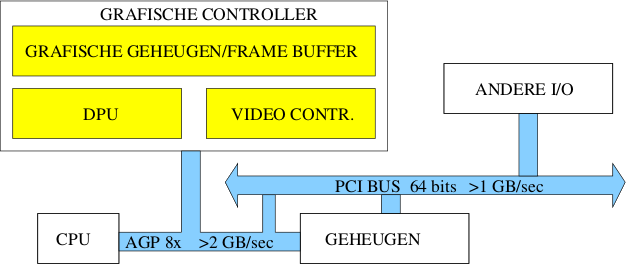
\includegraphics[scale=0.4, angle=0]{plaatjes/agp.png}}
		\end{center}
		
		
		
		In plaats van \verb!scale=x! kan je beter de relatieve afmeting
		\verb!width=\Procent{y}! gebruiken. De waarde $y$ wordt in de
		verslag-mode met uitproberen gevonden, zie figuur~\ref{fig:PDFR}.
		
		\begin{center}
			
			%	\figuur{width=\columnwidth}{plaatjes/2020/eerste oplevermoment/knop.png}{PNGR}{Variabele breedte (png)}
			\subfloat[The net of (c) after firing]{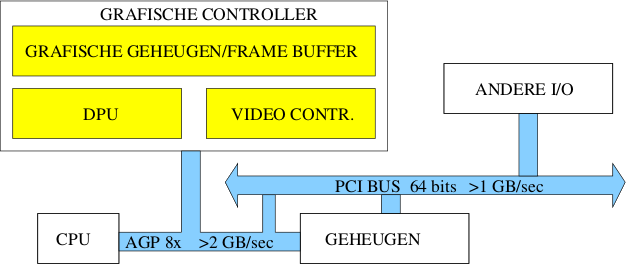
\includegraphics[scale=0.4, angle=0]{plaatjes/agp.png}}
		\end{center}
		
		
		Het afmetingsprobleem is iets gemakkelijker op te lossen met `bitmap
		graphics' van het `jpg-', `gif-' en `png-' formaat omdat de figuren al
		van te voren geschaald kunnen worden als de `bounding box' bij het
		inlezen bekend is. De breedte (\verb!width!) kan als percentage van de
		kolombreedte (\verb!width=\Procent{0 ... 99}!) worden opgegeven zoals
		dat bij figuur~\ref{fig:PNGR} gedaan is. Voor een 100\% waarde neemt
		men \verb!width=\columnwidth! De afmeting wordt automatisch
		aangepast aan de nieuwe kolombreedte.
		
		
		
		\begin{center}
			\begin{tabular}{|>\C p{\Procent{80}}|}
				\hline
				~\\
				Use case\\
				~\\
				Wachten voor de sluis\\
				~\\
				\hline
			\end{tabular}
		\end{center}
		
		
		
		
		\begin{center}
			\begin{tabular}{|>\C p{\Procent{80}}|}
				\hline
				~\\
				Use case\\
				~\\
				Sluis invaren\\
				~\\
				\hline
			\end{tabular}
		\end{center}
		
		
		
		
		
		\begin{center}
			\begin{tabular}{|>\C p{\Procent{80}}|}
				\hline
				~\\
				Use case\\
				~\\
				Sluis uitvaren\\
				~\\
				\hline
			\end{tabular}
		\end{center}
		
		\begin{center}
			
			\subfloat[The net of (c) after firing]{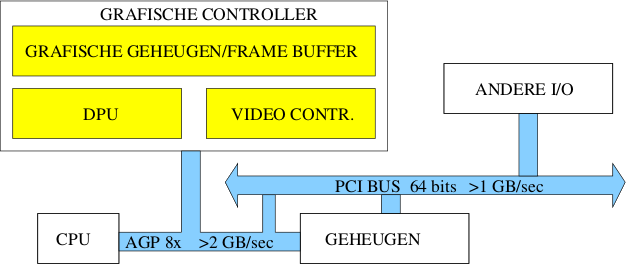
\includegraphics[scale=0.4, angle=0]{plaatjes/agp.png}}
		\end{center}
		
		\begin{center}
			
			\subfloat[The net of (c) after firing]{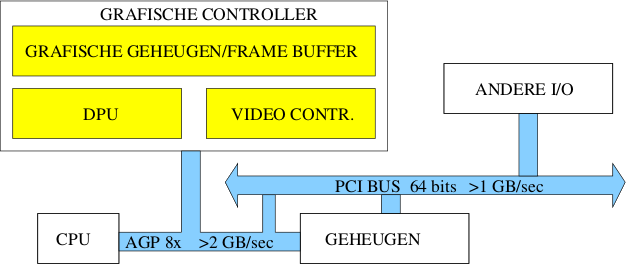
\includegraphics[scale=0.4, angle=0]{plaatjes/agp.png}}
		\end{center}
		
		\begin{center}
			
			\subfloat[The net of (c) after firing]{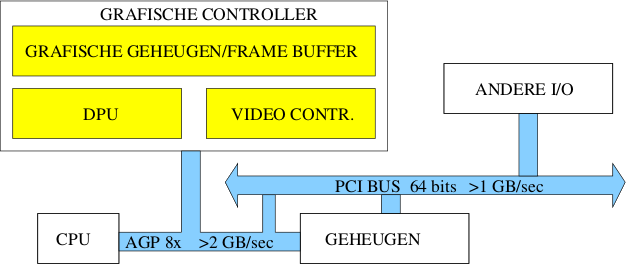
\includegraphics[scale=0.4, angle=0]{plaatjes/agp.png}}
		\end{center}
		
		
		
		
		\begin{center}
			\begin{tabular}{|>\C p{\Procent{80}}|}
				\hline
				~\\
				Use case\\
				~\\
				Meerdere niveaus\\
				~\\
				\hline
			\end{tabular}
		\end{center}
		
		De macro \verb!\PROCENT{0...99}! is nodig voor de macro's \verb!Tabel!
		en \verb!Figuur!. Deze laatste twee macro's maken het mogelijk dat
		tabellen en afbeeldingen in de twocolumn-mode passen met behoud van
		hun originele afmeting en detaillering (zie
		figuur \ref{fig:FIXED}). De parameters van deze macro's komen overeen
		met de parameters van de macro's \verb!tabel! en \verb!figuur!.
		
		
		
		In het algemeen heeft vector-graphics een betere kwaliteit van de
		weergave dan bitmap-graphics.
		
		
		\paragraaf{Bijzondere tekens en afbreekproblemen}
		
		Bijzondere tekens zoals de á, à, ä, é, è, ë, ï, ü, ç \ldots worden
		probleemloos door \LaTeX{} geaccepteerd als normale utf8
		karakters. Voor de uitzonderingen bestaan macro's zoals het
		euro-symbool \euro{} waarvoor de macro \verb!\euro! nodig is. In
		wiskundige formules kan je gebruik maken van de macro \verb!\eurom!.
		
		
		In de two-columnmode zijn regels soms te lang als er gebruik gemaakt
		is van \verb!verb! of \verb!verbatim! of woorden die niet goed worden
		afgebroken. In dat laatste geval kan je in zo'n woord een afbreekpunt
		introduceren met de twee tekens \verb!\-!. Een regel kan gecontroleerd
		afgebroken door van te voren onzichtbare knikpunten te plaatsen met de
		\verb!\Knak! macro. De volgende regel moet in in tegenstelling met de
		twocolumnmode in de verslagmode ongeknakt worden weergegeven:
		
		\begin{Aanpassen}
			\begin{verbatim}
				... aaaaaaa\Knak{}aaaaaaa ...
			\end{verbatim}
		\end{Aanpassen}
		
		
		aaaaaaaaaaaaaaaaaaaaaaaaaaaaaaaaaaaaaaa\Knak{}aaaaaaaaaaaaaaaaaaaaaaaaaaaaaaaaaaaaaaa.
		
		Voor regels waarbij de structuur niet gebroken mag worden, is de
		\verb!\Knak!-methode ongeschikt, bijvoorbeeld bij scripts en
		broncode. Daarentegen zorgt de \verb!Aanpassen!-omgeving ervoor dat in
		de twocolumn-mode de regels met behoud van de originele structuur
		worden weergegeven. Daarvoor wordt een kleinere letterafmeting
		gebruikt (default de \verb!\scriptsize!). Deze omgeving werkt alleen
		met niet al te lange regels. Bij zeer lange regels moet de
		letterafmeting zeer klein worden waardoor de leesbaarheid in het
		gedrang komt. In dat geval moet naar een andere oplossing gezocht
		worden zoals het opnemen van de probleemregels (broncode en scripts)
		in de bijlagen.
		
		\begin{Aanpassen}[\tiny]
			aaaaaaaaaaaaaaaaaaaaaaaaaaaaaaaaaaaaaaaaaaaaaaaaaaaaaaaaaaaaaaaaaaaaaaaaaaaaaa.
		\end{Aanpassen}
		
		Hoewel het gebruik van opsommingen (\verb!\item!), letterlijke citaten
		\verb!quotation! en kaders (\verb!\fbox!) in de twocolumn-mode tot
		problemen kunnen leiden, zijn ze beperkt toegestaan. Bijvoorbeeld voor
		de kaders rond de teksten kan je beter gebruik maken van de
		\verb!tabular!-omgeving (of de \verb!tabel!-omgeving als je geen last
		wil hebben van pagina-overgangen), dan voor de standaard
		\verb!\fbox!-methode. De kolom van deze omkaderde tabel moeten dan wel
		een relatieve afmetingsverhouding de \verb!\columnwidth! krijgen.
		
		\begin{Aanpassen}
			\begin{verbatim}
				\begin{center}
					\begin{tabular}{|>\C p{\Procent{80}}|}
						\hline
						Afbreekproblemen ...
						\hline
					\end{tabular}
				\end{center}
			\end{verbatim}
		\end{Aanpassen}
		
		\begin{center}
			\begin{tabular}{|>\C p{\Procent{80}}|}
				\hline
				~\\
				Afbreek- en andere opmaakproblemen pak je als laatste aan,
				dus bij je definitieve verslag!\\
				~\\
				Tabellen, figuren en listingen in het hoofdverslag tot het
				noodzakelijke beperken.\\
				~\\
				\hline
			\end{tabular}
		\end{center}
		
		
		\paragraaf{Algoritmen en broncode\cite{wikibooks}}
		
		Als je algoritmen met een mooie layout wilt hebben, dan zou je het
		\verb!algorithmic!-pakket kunnen gebruiken. Met dit pakket kan je het
		algoritme op een logische manier opbouwen met pseudotaal. Het bestand
		`verslag.tex' bevat al de pakketten \verb!algorithmic! en
		\verb!listings! die voor dit verslag nodig zijn. Als je zelf packages
		wil toevoegen of verwijderen (afblijven van
		\verb!\usepackage{moduleverslag}!)  dan moet dat in de preambule
		`verslag.tex'.
		
		\begin{Aanpassen}
			\begin{verbatim}
				\usepackage{algorithmic}
			\end{verbatim}
		\end{Aanpassen}
		
		Een algoritme moet je maken binnen een algorithmic-omgeving, een
		voorbeeld:
		
		\begin{Aanpassen}[\small]
			\begin{algorithmic}
				\IF {$i\geq maxval$} 
				\STATE $i\gets 0$
				\ELSE
				\IF {$i+k\leq maxval$}
				\STATE $i\gets i+k$
				\ENDIF
				\ENDIF 
			\end{algorithmic}
		\end{Aanpassen}
		
		
		Broncode kan je in een \verb!verbatim!-omgeving opnemen. De
		broncoderegels zien er net zo uit zoals je ze ingetypt hebt.  Het
		\verb!listings!-pakket is geavanceerder dan de
		\verb!verbatim!-omgeving.
		
		\begin{Aanpassen}
			\begin{verbatim}
				\usepackage{listings}
			\end{verbatim}
		\end{Aanpassen}
		
		Merk even op dat alle commando's van het \verb!listings!-pakket
		beginnen met \verb!lst!, dit conform de lppl-licentie.
		
		De broncode zelf zet je in een \verb!listings!-omgeving, net zoals bij
		de \verb!verbatim!-omgeving, om broncode te zetten gebruik je het
		\verb!\lstinline!-commando op dezelfde manier als het
		\verb!\verb!-commando. Je kunt ook broncode van een extern document laden met het commando:
		
		\begin{Aanpassen}
			\begin{verbatim}
				\lstinputlisting{pathname}
			\end{verbatim}
		\end{Aanpassen}
		
		Het argument `pathname' is de relatieve of absolute locatie van het
		bronbestand, de map(pen) gecombineerd met de bestandsnaam. Als je
		broncode van een bronbestand laadt, ben je zeker dat de broncode in je
		\LaTeX{}-document altijd actueel is en hou je het \LaTeX{}-document
		overzichtelijk. Als de broncode niet in dezelfde map of een submap van
		het \LaTeX{}-document staat of je gebruikt absolute `pathnames', dan
		is het mogelijk dat het verslag niet op andere computers gecompileerd
		kan worden. Bij het inleveren van je afstudeerverslag in
		\LaTeX{}-formaat zal je hiermee rekening moeten houden.
		
		
		Alle opties in het \verb!listings!-pakket hebben eenzelfde structuur
		\verb!sleutel=waarde!. Als je alleen 'Java' gebruikt hebt, dan kan je
		deze taal voor je volledig document na de regel
		\verb!\usepackage{listings}! in preambule `verslag.tex' definiëren met
		\verb!\lstset{language=java}!
		
		\lstset{language=java}
		
		\begin{Aanpassen}
			\begin{lstlisting}
				public class HelloWorld {
					public static void main(String[] args) {
						System.out.println("Hello, world!");
					}
				}
			\end{lstlisting}
		\end{Aanpassen}
		
		
		De sleutel is hier dus \verb!language! en de waarde die je aan de
		sleutel geeft is \verb!java!. Alles wat je als opties binnen de
		\verb!\lstset!-macro zet kan je per \verb!listings!-omgeving apart
		definiëren. Bijvoorbeeld html-broncode met
		\verb!\begin{lstlisting}[language=html]!:
			
			\begin{Aanpassen}
				\begin{lstlisting}[language=html]
					<html>
					<head>
					<title>Hello</title>
					</head>
					<body>Hello</body>
					</html>
				\end{lstlisting}
			\end{Aanpassen}
			
			\subsection{Conclusie}
			
			
			
			Om een goed verhaal op te stellen, moet vooraf aan enkele voorwaarden
			worden voldaan. De eerste voorwaarde is de geschiktheid van het
			afstudeerproject. Als een afstudeerproject niet tot keuzes leidt, kan
			men zich afvragen of dat wel een echte afstudeeropdracht is. Een
			afstudeerproject zonder onderzoeksaspecten is ook verdacht. Daarnaast
			moet een afstudeerproject passen in het profiel van een opleiding om
			beoordeelbaar te zijn. De andere voorwaarde voor goed een verhaal is
			de registratie van werkzaamheden tijdens het a
			worden voldaan. De eerste voorwaarde is de geschiktheid van het
			afstudeerproject. Als een afstudeerproject niet tot keuzes leidt, kan
			men zich afvragen of dat wel een echte afstudeeropdracht is. Een
			afstudeerproject zonder onderzoeksaspecten is ook verdacht. Daarnaast
			moet een afstudeerproject passen in het profiel van een opleiding om
			beoordeelbaar te zijn. De andere voorwaarde voor goed een verhaal is
			de registratie van werkzaamheden tijdens het a
			
			
			Subheadings reflect the content and organization of the different parts of the main text. Each paragraph may cover one idea, characteristic or topic. Don’t refer only one study in each paragraph.Wherever required, link the research findings to the research problem described in the introduction. Three tenses (simple present, simple past and present perfect) are frequently used. Length of this section is about 70% to 90% of main text.
			
			
			22)   Present your results in logical sequence  in the text,tables and illustrations.  Do not repeat in the text all the data, in the tables or illustrations.
			23)   Emphasize or summarize important observations.Results  section should contain only  actuals, and no opinions.
			24)   All  the  patients  included  in  the  study  should  be accounted for. There should not be any hesitation in reporting any negative or unexpected result.
			
			
			
			\begin{figure}[!ht]
				\centering
				\begin{floatrow}
					\ffigbox[\FBwidth]{\caption{Dummy figure}\label{fig:dummy-1}}{%
						\rule{1.6in}{0.9in}   % Just a dummy. Replace with your figure.
					}
					\ffigbox[\FBwidth]{\caption{Dummy figure}\label{fig:dummy-2}}{%
						\rule{1.6in}{0.9in}   % Just a dummy. Replace with your figure.
					}
					
					\ffigbox[\FBwidth]{\caption{Dummy figure}\label{fig:dummy-1}}{%
						\rule{1.6in}{0.9in}   % Just a dummy. Replace with your figure.
					}
					\ffigbox[\FBwidth]{\caption{Dummy figure}\label{fig:dummy-2}}{%
						\rule{1.6in}{0.9in}   % Just a dummy. Replace with your figure.
					}
				\end{floatrow}
			\end{figure}
			
			
			\begin{figure}[!tbp]
				\centering
				\subfloat[Flower one.]{\includegraphics[width=0.4\textwidth]{flower1.jpg}\label{fig:f1}}
				\hfill
				\subfloat[Flower two.]{\includegraphics[width=0.4\textwidth]{flower2.jpg}\label{fig:f2}}
				\caption{My flowers.}
				\subfloat[Flower one.]{\includegraphics[width=0.4\textwidth]{flower1.jpg}\label{fig:f1}}
				\hfill
				\subfloat[Flower two.]{\includegraphics[width=0.4\textwidth]{flower2.jpg}\label{fig:f2}}
				\caption{My flowers.}
			\end{figure}
			
			
			
			\section{testresultaten}
			Om een goed verhaal op te stellen, moet vooraf aan enkele voorwaarden
			worden voldaan. De eerste voorwaarde is de geschiktheid van het
			afstudeerproject. Als een afstudeerproject niet tot keuzes leidt, kan
			men zich afvragen of dat wel een echte afstudeeropdracht is. Een
			afstudeerproject zonder onderzoeksaspecten is ook verdacht. Daarnaast
			moet een afstudeerproject passen in het profiel van een opleiding om
			beoordeelbaar te zijn. De andere voorwaarde voor goed een verhaal is
			de registratie van werkzaamheden tijdens het a
			
			
			\begin{tabular}{|l|l {2cm} |l|l|l|l|l|l|l|l|} \hline
				\multicolumn{10}{|l|}{REQ traceabilitymatrix}                                                               \\ \hline
				\multicolumn{4}{|l|}{project name}   &\multicolumn{6}{|l|}{Created designed by}                           \\ \hline
				\multicolumn{4}{|l|}{release no}   &\multicolumn{6}{|l|}{Created on}                           \\ \hline
				\multicolumn{4}{|l|}{version}   &\multicolumn{6}{|l|}{Reviewed on}                           \\ \hline
				\multicolumn{4}{|l|}{Test title}   &\multicolumn{6}{|l|}{Reviewed by}                           \\ \hline
				\multicolumn{4}{|l|}{Description}   &\multicolumn{6}{|l|}{ }                           \\ \hline 		
				\multicolumn{10}{|l|}{ }   																\\ \hline
				\multicolumn{10}{|l|}{Pre condition}                                                               \\ \hline
				\multicolumn{10}{|l|}{Dependencies}                                                               \\ \hline
				\multicolumn{10}{|l|}{ }   															\\ \hline
				\multicolumn{2}{|l|}{REQ ID} & description & Status &Designdoc &codemodule&testaseID &T.case Name & manual& testedon \\ \hline
				\multicolumn{2}{|l|}{REQ ID} &  \thead{ Als  \\gebruiker \\	wil ik  \\een  \\ 	ssid  \\invoeren   }
				& Status &Designdoc &codemodule&testaseID &T.case Name & manual& testedon \\ \hline
				\multicolumn{2}{|l|}{REQ ID} &  \thead{ Als  \\gebruiker \\	wil ik  \\een  \\ 	ssid  \\invoeren   }
				& Status &Designdoc &codemodule&testaseID &T.case Name & manual& testedon \\ \hline
				\multicolumn{2}{|l|}{REQ ID} &  \thead{ Als  \\gebruiker \\	wil ik  \\een  \\ 	ssid  \\invoeren   }
				& Status &Designdoc &codemodule&testaseID &T.case Name & manual& testedon \\ \hline
				\multicolumn{2}{|l|}{REQ ID} &  \thead{ Als  \\gebruiker \\	wil ik  \\een  \\ 	ssid  \\invoeren   }
				& Status &Designdoc &codemodule&testaseID &T.case Name & manual& testedon \\ \hline
			\end{tabular}
			
			
			
			
			
			
			
			\subsection{Testcases}		
			
			Om een goed verhaal op te stellen, moet vooraf aan enkele voorwaarden
			worden voldaan. De eerste voorwaarde is de geschiktheid van het
			afstudeerproject. Als een afstudeerproject niet tot keuzes leidt, kan
			men zich afvragen of dat wel een echte afstudeeropdracht is. Een
			afstudeerproject zonder onderzoeksaspecten is ook verdacht. Daarnaast
			moet een afstudeerproject passen in het profiel van een opleiding om
			beoordeelbaar te zijn. De andere voorwaarde voor goed een verhaal is
			de registratie van werkzaamheden tijdens het a
			
			
			
			\begin{tabular}{|l|l|l|l|l|l|l|} \hline
				\multicolumn{7}{|l|}{project name}                                                               \\ \hline
				\multicolumn{4}{|l|}{Test case ID}   &\multicolumn{3}{|l|}{Test designed by}                           \\ \hline
				\multicolumn{4}{|l|}{test priority (low/medium/high)}   &\multicolumn{3}{|l|}{Test design date}                           \\ \hline
				\multicolumn{4}{|l|}{Module name}   &\multicolumn{3}{|l|}{Test executed by}                           \\ \hline
				\multicolumn{4}{|l|}{Test title}   &\multicolumn{3}{|l|}{Test execution date}                           \\ \hline
				\multicolumn{4}{|l|}{Description}   &\multicolumn{3}{|l|}{ }                           \\ \hline 		
				\multicolumn{7}{|l|}{ }   																\\ \hline
				\multicolumn{7}{|l|}{Pre condition}                                                               \\ \hline
				\multicolumn{7}{|l|}{Dependencies}                                                               \\ \hline
				\multicolumn{7}{|l|}{ }   															\\ \hline
				Step  &  Test steps & Test data & expected result &Acual result &Streee (pass or fail)&notes  \\ \hline
				
			\end{tabular}
			
			
			
			
			
			
			
			\subsection{Reparaties}
			
			\subsection{Resulaat annalyse}
			
			\lipsum[2-4]
			\begin{figure}[t]
				\centering
				\subfloat[Net is not enabled because multiplicity of read arc $<2$] {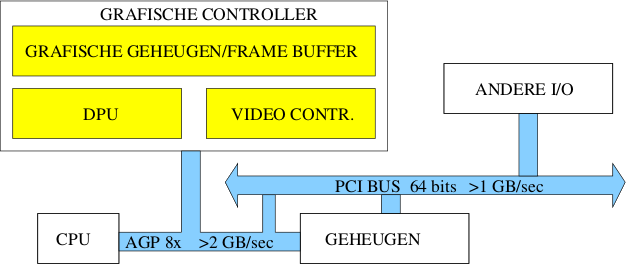
\includegraphics[scale=0.4, angle=0]{plaatjes/agp.png}}\hfil
				\subfloat[Net is not enabled C $>1$] {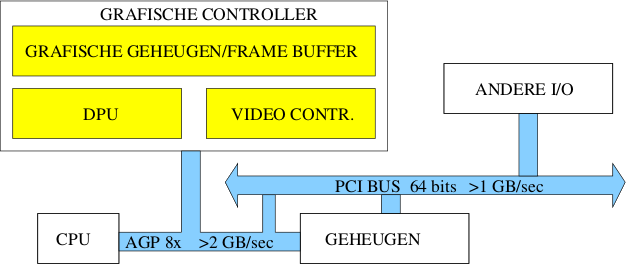
\includegraphics[scale=0.4, angle=0]{plaatjes/agp.png}}
				
				\subfloat[The net is enabled]{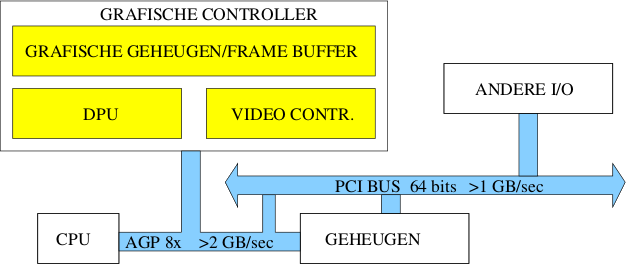
\includegraphics[scale=0.4, angle=0]{plaatjes/agp.png}}\hfil
				\subfloat[The net of (c) after firing]{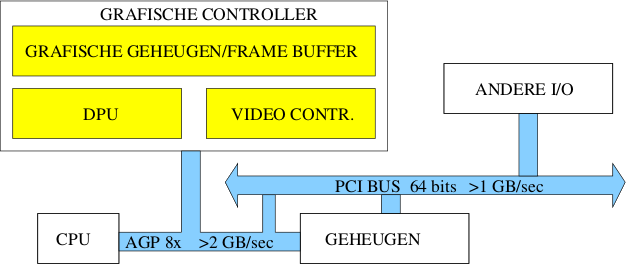
\includegraphics[scale=0.4, angle=0]{plaatjes/agp.png}}
				\caption{}
				
				
				\label{fig: 2.2}
			\end{figure}
			
			
			\subsection{Reparaties}
			
			\subsection{Resulaat annalyse}
			
			\lipsum[2-4]
			\begin{figure}[t]
				\centering
				\subfloat[Net is not enabled because multiplicity of read arc $<2$] {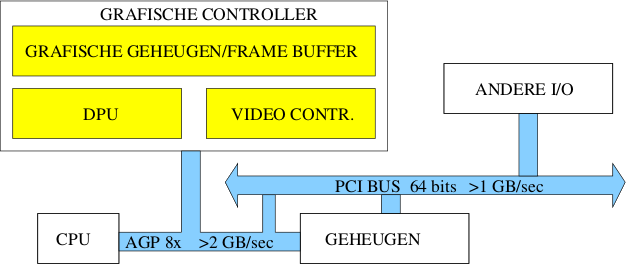
\includegraphics[scale=0.4, angle=0]{plaatjes/agp.png}}\hfil
				\subfloat[Net is not enabled C $>1$] {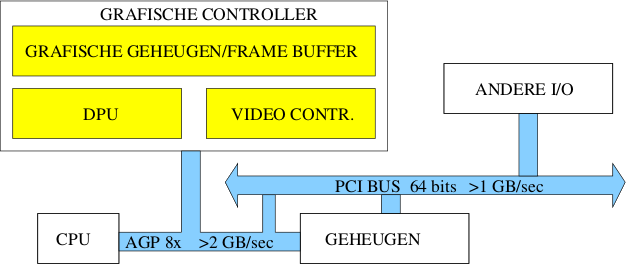
\includegraphics[scale=0.4, angle=0]{plaatjes/agp.png}}
				
				\subfloat[The net is enabled]{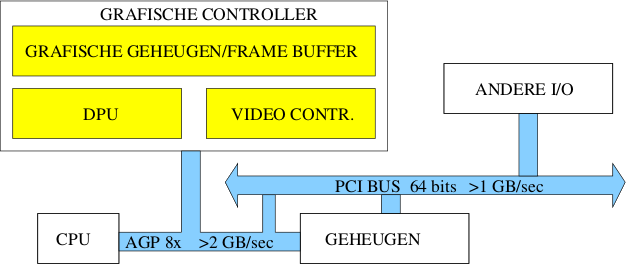
\includegraphics[scale=0.4, angle=0]{plaatjes/agp.png}}\hfil
				\subfloat[The net of (c) after firing]{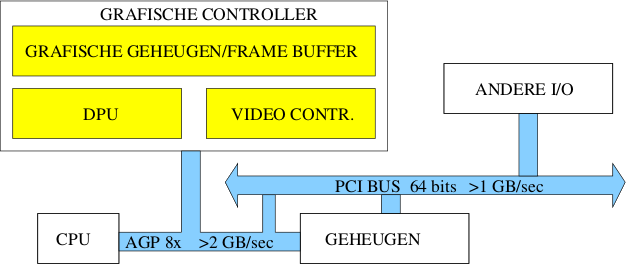
\includegraphics[scale=0.4, angle=0]{plaatjes/agp.png}}
				\caption{}
				
				
				\label{fig: 2.2}
			\end{figure}
			
			%%%%%%%%%%%%%%%%%%%%%%%%%%%%%%%%%%%%%%%%%%%%%%%%%%%%%%%%%%%%%%
   


\subsubsection{Ramp schietpartij militair ossendrecht }
Een militaire overleid op een schietbaan in ossendracht door onvoldoende begeleiding van cursisten, geen toezicht op de lokatie. E\r was een instructuur in opleiding die niet volledig was mmeegenomen in het poroces en ook was er geen baancommandant aanwezig. Geen van de aanwezig instructeurts had de juiste papieren om de cursisten te begeleiden. De aanwezig instruceur had geen zich op de instructeur in opleiding, evenmin de andere militairen. In de instructiehandleiding ontbreken richtlijnen voor bijzondere schietbanen. Ook was er geen keuring. Door personelstekort is er geen andacht besteed aan documentastie(een slyllabus) hoe en met welke risico’s oefeningnen moeten worden ingericht. Ok werd er vooraf geen veiliheidsanaklyse gedaan. Het gebrek aan lesmateriaal en deskundigen is gemeld binnen de defensieorganisatie maar dit heeft niet geleid tot enige verandering in de situatie.
Op een afgekeurde scheitbaan
Tezicht door een instructeur in opleiding die zelf geen persoonlijke begeleiding heeft gehad tijdens de uitvoering
Belangrijk is dat defensie haar taken kan uitvoeren met personeel dat is getraind in situaties die de risicos van de werkomgeving aan de cursisten kunnen laten zien.
Conclusie
Zonder gekwalificeerde instructuers.
Zonder toezicht
Zonder lesmateriaal
Zonder adequate veiligheidsanalyse
https://www.youtube.com/watch?v=6jmkDClGDHo    



\subsubsection{schipholbrand}
Om een goed verhaal op te stellen, moet vooraf aan enkele voorwaarden
worden voldaan. De eerste voorwaarde is de geschiktheid van het
afstudeerproject. Als een afstudeerproject niet tot keuzes leidt, kan
men zich afvragen of dat wel een echte afstudeeropdracht is. Een
afstudeerproject zonder onderzoeksaspecten is ook verdacht. Daarnaast
moet een afstudeerproject passen in het profiel van een opleiding om
beoordeelbaar te zijn. De andere voorwaarde voor goed een verhaal is
de registratie van werkzaamheden tijdens het a   



\subsubsection{slmramp}
Toen de Anthony Nesty Zanderij naderde, was het daar, anders dan het weerbericht had voorspeld, mistig. Het zicht was evenwel niet zo slecht dat er niet op zicht kon worden geland. Gezagvoerder Will Rogers besloot echter via het Instrument Landing System (ILS) te landen, hoewel dit niet betrouwbaar was en hij voor zo'n landing ook geen toestemming had. De gezagvoerder brak drie landingspogingen af. Bij de vierde poging negeerde de bemanning de automatische waarschuwing (GPWS) dat het toestel te laag vloog. Het toestel raakte op 25 meter hoogte twee bomen. Het rolde om de lengteas en stortte om 04.27 uur plaatselijke tijd ondersteboven neer.

Uit onderzoek bleek dat de papieren van de bemanning niet in orde waren. 
Geconcludeerd werd dat de gezagvoerder roekeloos had gehandeld door voor een ILS-landing te kiezen terwijl hij daar geen toestemming voor had, en door onvoldoende op de vlieghoogte te hebben gelet. 
De SLM werd verweten de kwalificaties van de bemanning onvoldoende te hebben gecontroleerd.

https://aviation-safety.net/investigation/cvr/transcripts/cvr_py764.php 
https://aviation-safety.net/database/record.php?id=19890607-2    



\subsubsection{stint ongeluk}
Vier kinderen, een bestuurder kwamen om en een vijfde persoon , een kind raakte zwaargewond. Uit odnerzoek van bleek :
Foute torsieveer voor de gashendel werd geleverd
Geen van de drie onderzochte voertuigen haalden de wettelijk vereiste remvertraging
De automatische parkeerrem kan leiden tot gevaarlijke situaties wanneer deze ongewenst geactiveerd wordt tijdens het rijden. 
Het losraken van de nuldraad naar de gashendel leidt volgens TNO tot ongewenst versnellen van het voertuig en een oncontroleerbare situatie voor de bestuurder.
Voor alle drie onderzochte voertuigen geldt dat het ontbreken van een zitplaats leidt tot veiligheidsrisico’s voor remmen en sturen door de grotere kans dat de bestuurder van het voertuig valt. Als de bestuurder van een Stint valt, leidt dit in alle rijsituaties tot een onbeheersbare situatie


https://repository.tno.nl/islandora/object/uuid%3Acdef48df-da49-46b6-8678-5c62a88a0090 
   


\section{tesla crash report}
Door een softwarefout zijn er situaties ontstaan waarin het systeem informatie een onvoldoende informatie positie had om de juiste beslissingen te maken. Of dat de informatieverwerking niet juist was.












hardware/software/gebruik

How does Tesla use Big data?
In general, tesla autonomous vehicle technology should be able to do some of the following things:

· Sense plan act: In order to make sure of the plan and act, the vehicle machine learning algorithms must be able to predict the outcomes which are based on a high volume of data.

· Mapping: The vehicle computer must possess highly detailed, comprehensive maps of street features, which includes the signs, streetlights, and curbs.

· Light detection and ranging: Using the sensors such as the LIDAR and cameras, the vehicle should be able to create a short distance readout of its surrounding in the real-time scenario.

· Vehicle to Vehicle communication: Tesla autonomous vehicle technology does not have this up and running yet, but the best-case scenario would even involve an Internet of Things aspect, in which all the autonomous vehicle is communicating some of the essential details to each other. Projections show that more than 400 million smart cars will be a part of the IoT by the end of 2021.


Tesla Machine learning in the cloud is responsible to takes care of educating the entire set of the fleet, while at an individual car level, some of the edge computing decides what action the car needs to take right now. The third level of decision making also exists, with cars able to form networks with some other Tesla vehicles nearby to make sure in order to share some of the local insights and information.

In near future scenario where the autonomous cars are widespread, these networks will most likely also interface with cars from some other manufacturers as well as other systems such as road-based sensors, traffic camera, purge light up mask or smartphones.

Although details are scarce on the new Artificial Intelligence technology that Tesla was creating, its current AI – which is driven by a collaboration with the hardware manufacturer Nvidia, that is even largely based on a model of an unsupervised model of machine learning.

On its Facebook page, Nvidia state that “In contrast to the usual approach to operating self-driving cars, we did not program any explicit object detection, mapping, path planning or control components into this car. Instead, the car learns on its own to create all necessary internal representations necessary to steer, simply by observing human drivers.”

https://www.techiexpert.com/how-tesla-is-using-artificial-intelligence-and-big-data/

Notably, Tesla says this silicon, with its twin neural network arrays capable of 36 trillion operations per second (each), will only cost the company 80 percent of what it was paying before for that 21x performance gain, and draw little enough additional wattage (72W, vs. 57W) that it can continue to promise the same range out of each car and without impacting the cost.
https://www.theverge.com/2019/4/22/18511594/tesla-new-self-driving-chip-is-here-and-this-is-your-best-look-yet

ChipIptimalisatie met NVideai:
The road to this success was through a huge number of transistors- 6 billion to be precise.
Dual Chips for Better Control
Tesla AI chips Optimised Design
Tesla AI chips have been optimised to perform 36 trillion operations per second and runs ar 2GHs. This high level of performance has been achieved by eliminating generic functions and focusing only on specific important ones.
https://www.mygreatlearning.com/blog/teslas-new-ai-for-self-driving-cars/

the NVIDIA DRIVE PX2 driverless car platform
can perform 30 trillion deep learning operations per second and can achieve Level4 autopilot [21].
It supports 12-channel camera inputs, laser positioning, radar, and ultrasonic sensors, and includes
two new-generation NVIDIA Tegra processors (see Figure 4). When it comes to softwares, Tensorflow
is one of the main libraries for deep learning used in the field of self-driving cars

Convolutional Neural Network
Recurrent Neural Network
Auto-Encoder (AE)
Deep Reinforcement Learning (DRL)
Obstacle Detection
Lane Recognition
path planning, motion control, pedestrian detection,
and traffic sign and light detection


file:///C:/Users/gally/Downloads/applsci-10-02749-v2.pdf

The hardware and software of self-driving cars
Another important point Musk raised in his remarks is that he believes Tesla cars will achieve level 5 autonomy “simply by making software improvements.”

Other self-driving car companies, including Waymo and Uber, use lidars, hardware that projects laser to create three-dimensional maps of the car’s surroundings. Tesla, on the other hand, relies mainly on cameras powered by computer vision software to navigate roads and streets. Tesla use deep neural networks to detect roads, cars, objects, and people in video feeds from eight cameras installed around the vehicle. (Tesla also has a front-facing radar and ultrasonic object detectors, but those have mostly minor roles.)

There’s a logic to Tesla’s computer vision–only approach: We humans, too, mostly rely on our vision system to drive. We don’t have 3D mapping hardware wired to our brains to detect objects and avoid collisions.

But here’s where things fall apart. Current neural networks can at best replicate a rough imitation of the human vision system. Deep learning has distinct limits that prevent it from making sense of the world in the way humans do. Neural networks require huge amounts of training data to work reliably, and they don’t have the flexibility of humans when facing a novel situation not included in their training data.

This is something Musk tacitly acknowledged at in his remarks. “[Tesla Autopilot] does not work quite as well in China as it does in the U.S. because most of our engineering is in the U.S.” This is where most of the training data for Tesla’s computer vision algorithms come from.

Deep learning’s long-tail problem
Human drivers also need to adapt themselves to new settings and environments, such as a new city or town, or a weather condition they haven’t experienced before (snow- or ice-covered roads, dirt tracks, heavy mist). However, we use intuitive physics, commonsense, and our knowledge of how the world works to make rational decisions when we deal with new situations.

We understand causality and can determine which events cause others. We also understand the goals and intents of other rational actors in our environments and reliably predict what their next move might be. For instance, if it’s the first time that you see an unattended toddler on the sidewalk, you automatically know that you have pay extra attention and be careful. And what if you meet a stray elephant in the street for the first time? Do you need previous training examples to know that you should probably make a detour?

But for the time being, deep learning algorithms don’t have such capabilities, therefore they need to be pre-trained for every possible situation they encounter.

There’s already a body of evidence that shows Tesla’s deep learning algorithms are not very good at dealing with unexpected scenery even in the environments that they are adapted to. In 2016, a Tesla crashed into a tractor-trailer truck because its AI algorithm failed to detect the vehicle against the brightly lit sky. In another incident, a Tesla self-drove into a concrete barrier, killing the driver. And there have been several incidents of Tesla vehicles on Autopilot crashing into parked fire trucks and overturned vehicles. In all cases, the neural network was seeing a scene that was not included in its training data or was too different from what it had been trained on.

If there’s one company that can solve the self-driving problem through data from the real world, it’s probably Tesla. The company has a very comprehensive data collection program—better than any other car manufacturer doing self-driving software of software company working on self-driving cars. It is constantly gathering fresh data from the hundreds of thousands of cars it has sold across the world and using them to fine-tune its algorithms.

But will more data solve the problem?
Interpolation vs extrapolation
The AI community is divided on how to solve the “long tail” problem. One view, mostly endorsed by deep learning researchers, is that bigger and more complex neural networks trained on larger data sets will eventually achieve human-level performance on cognitive tasks. The main argument here is that the history of artificial intelligence has shown that solutions that can scale with advances in computing hardware and availability of more data are better positioned to solve the problems of the future.

This is a view that supports Musk’s approach to solving self-driving cars through incremental improvements to Tesla’s deep learning algorithms. Another argument that supports the big data approach is the “direct-fit” perspective. Some neuroscientists believe that the human brain is a direct-fit machine, which means it fills the space between the data points it has previously seen. The key here is to find the right distribution of data that can cover a vast area of the problem space.

If these premises are correct, Tesla will eventually achieve full autonomy simply by collecting more and more data from its cars. But it must still figure out how to use its vast store of data efficiently.


On the opposite side are those who believe that deep learning is fundamentally flawed because it can only interpolate. Deep neural networks extract patterns from data, but they don’t develop causal models of their environment. This is why they need to be precisely trained on the different nuances of the problem they want to solve. No matter how much data you train a deep learning algorithm on, you won’t be able to trust it, because there will always be many novel situations where it will fail dangerously.

The human mind on the other hand, extracts high-level rules, symbols, and abstractions from each environment, and uses them to extrapolate to new settings and scenarios without the need for explicit training.

I personally stand with the latter view. I think without some sort of abstraction and symbol manipulation, deep learning algorithms won’t be able to reach human-level driving capabilities.

There are many efforts to improve deep learning systems. One example is hybrid artificial intelligence, which combines neural networks and symbolic AI to give deep learning the capability to deal with abstractions.

Another notable area of research is “system 2 deep learning.” This approach, endorsed by deep learning pioneer Yoshua Bengio, uses a pure neural network–based approach to give symbol-manipulation capabilities to deep learning. Yann LeCun, a longtime colleague of Bengio, is working on “self-supervised learning,” deep learning systems that, like children, can learn by exploring the world by themselves and without requiring a lot of help and instructions from humans. And Geoffrey Hinton, a mentor to both Bengio and LeCun, is working on “capsule networks,” another neural network architecture that can create a quasi-three-dimensional representation of the world by observing pixels.

These are all promising directions that will hopefully integrate much-needed commonsense, causality, and intuitive physics into deep learning algorithms. But they are still in the early research phase and are not nearly ready to be deployed in self-driving cars and other AI applications. So I suppose they will be ruled out for Musk’s “end of 2020” timeframe.

believe the sample size and data distribution does not paint an accurate picture yet.

But more importantly, I think comparing numbers is misleading at this point. What is more important is the fundamental difference between how humans and AI perceive the world.

Our eyes receive a lot of information, but our visual cortex is sensible to specific things, such as movement, shapes, specific colors and textures. Through billions of years of evolution, our vision has been honed to fulfill different goals that are crucial to our survival, such as spotting food and avoiding danger.

But perhaps more importantly, our cars, roads, sidewalks, road signs, and buildings have evolved to accommodate our own visual preferences. Think about the color and shape of stop signs, lane dividers, flashers, etc. We have made all these choices—consciously or not—based on the general preferences and sensibilities of the human vision system.

Therefore, while we make a lot of mistakes, our mistakes are less weird and more predictable than the AI algorithms that power self-driving cars. Case in point: No human driver in their sane mind would drive straight into an overturned car or a parked firetruck.

Other problems that need to be solved
Given the differences between human and cop, we either have to wait for AI algorithms that exactly replicate the human vision system (which I think is unlikely any time soon), or we can take other pathways to make sure current AI algorithms and hardware can work reliably.

One such pathway is to change roads and infrastructure to accommodate the hardware and software present in cars. For instance, we can embed smart sensors in roads, lane dividers, cars, road signs, bridges, buildings, and objects. This will allow all these objects to identify each other and communicate through radio signals. Computer vision will still play an important role in autonomous driving, but it will be complementary to all the other smart technology that is present in the car and its environment. This is a scenario that is becoming increasingly possible as 5G networks are slowly becoming a reality and the price of smart sensors and internet connectivity decreases.

Just as our roads evolved with the transition from horses and carts to automobiles, they will probably go through more technological changes with the coming of software-powered and self-driving cars. But such changes require time and huge investments from governments, vehicle manufacturers, and well as the manufacturers of all those other objects that will be sharing roads with self-driving cars. And we’re still exploring the privacy and security threats of putting an internet-connected chip in everything.

An intermediate scenario is the “geofenced” approach. Self-driving technology will only be allowed to operate in areas where its functionality has been fully tested and approved, where there’s smart infrastructure, and where the regulations have been tailored for autonomous vehicles (e.g., pedestrians are not allowed on roads, human drivers are limited, etc.). Some experts describe these approaches as “moving the goalposts” or redefining the problem, which is partly correct. But given the current state of deep learning, the prospect of an overnight rollout of self-driving technology is not very promising. Such measures could help a smooth and gradual transition to autonomous vehicles as the technology improves, the infrastructure evolves, and regulations adapt.

There are also legal hurdles. We have clear rules and regulations that determine who is responsible when human-driven cars cause accidents. But self-driving cars are still in a gray area. For now, drivers are responsible for their Tesla’s actions, even when it is in Autopilot mode. But in a level 5 autonomous vehicle, there’s no driver to blame for accidents. And I don’t think any car manufacturer would be willing to roll out fully autonomous vehicles if they would to be held accountable for every accident caused by their cars.

https://bdtechtalks.com/2020/07/29/self-driving-tesla-car-deep-learning/

In fact, all Tesla vehicles – whether or not they are Autopilot enabled – send data directly to the cloud. A problem with the engine operation meaning that components were occasionally overheating was diagnosed in 2014 by monitoring this data and every vehicle was automatically “repaired” by software patch thanks to this.

Tesla effectively crowdsources its data from all of its vehicles as well as their drivers, with internal as well as external sensors which can pick up information about a driver’s hand placement on the instruments and how they are operating them. As well as helping Tesla to refine its systems, this data holds tremendous value in its own right. Researchers at McKinsey and Co estimate that the market for vehicle-gathered data will be worth $750 billion a year by 2030.

The data is used to generate highly data-dense maps showing everything from the average increase in traffic speed over a stretch of road to the location of hazards which cause drivers to take action. Machine learning in the cloud takes care of educating the entire fleet, while at an individual car level, edge computing decides what action the car needs to take right now. A third level of decision-making also exists, with cars able to form networks with other Tesla vehicles nearby in order to share local information and insights. In a near future scenario where autonomous cars are widespread, these networks will most likely also interface with cars from other manufacturers as well as other systems such as traffic cameras, road-based sensors or mobile phones.

https://www.forbes.com/sites/bernardmarr/2018/01/08/the-amazing-ways-tesla-is-using-artificial-intelligence-and-big-data/?sh=5e396aa24270


tesla model y
This autopilot is developed upon the principles of deep neural networks. It adopts cameras, ultrasonic sensors, and radar for perceiving the environment surrounding the vehicle.  These sensors and cameras allow the drivers to be receptive to their surroundings which are later on processed in a matter of milliseconds to aid in making the driving safer and less strenuous. The radar is adopted for seeing and measuring the distance around the cars in light, dark, and different weather conditions. The Ultraviolet techniques measure proximity in each case and the passive video detects objects around the car, ensuring a secure drive.
https://www.analyticssteps.com/blogs/how-tesla-making-use-artificial-intelligence-its-operations




4 variabelen model
Systemen (met daarin software) en de bijbehorende vier variabelen:
Monitored variabelen: door sensoren gekwanticeerdefenomenen uit de omgeving
Controlled variabelen: door actuatoren \bestuurde"fenomenen uit de omgeving


Input variabelen: data die de software als input gebruikt


According to Tesla, they have gathered data from over 100 million miles with their autopilot software. You can even find the best Halloween costumes on Purge Culture. This data are being compiled in the cloud to generate road maps for driverless cars which Tesla claims are 100 times more accurate than any standard navigation system.

https://www.techiexpert.com/how-tesla-is-using-artificial-intelligence-and-big-data/


Traffic Signs and Lights Recognition
In the traffic signs recognition, Xu et al. [82] proposed a traffic signs recognition approach based
on a CNN algorithm. First, the structural information of the traffic sign image is extracted based on the
hierarchical significance detection method. Then, a neural network model is used to extract the features
of the region of interest. Finally, the traffic sign is classified by the Softmax classifier to complete the
detection of the traffic sign. Alghmgham et al. [83] designed a deep-learning-based architecture and
applied it in the real-time traffic sign classification. The proposed architecture in [83] consists of two
convolutional layers, two max-pooling layers, one dropout layer and three dense layers.
In the traffic lights recognition, Lee and Kim [84] proposed a DNN-based method to detect traffic
lights in images. The detector in this paper has a DNN architecture of encoder-decoder. The encoder
is used to generate feature maps from the images by the ResNet-101. Then, the decoder is used to
generate a refined feature map from the results of the encoder, to output the final classification results
for the traffic lights. Kim et al. [85] proposed a traffic light recognition method based on deep learning,
which consists of a semantic segmentation network and a fully convolutional network. The semantic
segmentation network is employed to detect traffic lights and the fully convolutional network is used
for traffic light classification.

(1) The samples problem of deep learning
(2) The complexity problem of deep learning
(3) The robustness problem of deep learning.
(4) The real-time problem of deep learning
(5) The high-dimensional state-space problem of deep learning
(6) The 3D point cloud data processing based on deep learning
(7) The road support system based on deep learning
The ultimate goal for the development of self-driving cars is to build an automatic platform
capable of real-time, all-day and efficient driving service. Driverless technology can greatly improve
social productivity, generate huge social benefits, and improve the way people travel, to make a better
living environment. So there are lots of problems that need to be solved efficiently, which include two
sides, namely the applications of self-driving cars based on deep learning and the improvements of
deep learning algorithms. Thus, self-driving cars based on deep learning are still on the road.
file:///C:/Users/gally/Downloads/applsci-10-02749-v2.pdf

Path planning/driving policy
https://towardsdatascience.com/teslas-deep-learning-at-scale-7eed85b235d3

Using a variety of optimizations, Iandola and his co-authors demonstrated that they could achieve AlexNet-like performance while reducing the number of parameters by a factor of 50. That reduced the physical size of a trained AlexNet network from 240MB to less than 5MB. Using additional compression techniques developed by other researchers, including switching from 32-bit to 8-bit parameters, they were able to reduce the size of their model by another factor of 10—producing convolutional neural networks with AlexNet-like performance that were less than half a megabyte.

https://arstechnica.com/cars/2019/10/how-teslas-latest-acquisition-could-accelerate-autopilot-development/



In fact, all Tesla vehicles – whether or not they are Autopilot enabled – send data directly to the cloud. A problem with the engine operation meaning that components were occasionally overheating was diagnosed in 2014 by monitoring this data and every vehicle was automatically “repaired” by software patch thanks to this.

Tesla effectively crowdsouces its data from all of its vehicles as well as their drivers, with internal as well as external sensors which can pick up information about a driver’s hand placement on the instruments and how they are operating them. As well as helping Tesla to refine its systems, this data holds tremendous value in its own right. Researchers at McKinsey and Co estimate that the market for vehicle-gathered data will be worth $750 billion a year by 2030.

The data is used to generate highly data-dense maps showing everything from the average increase in traffic speed over a stretch of road, to the location of hazards which cause drivers to take action. Machine learning in the cloud takes care of educating the entire fleet, while at an individual car level, edge computing decides what action the car needs to take right now. A third level of decision-making also exists, with cars able to form networks with other Tesla vehicles nearby in order to share local information and insights. In a near future scenario where autonomous cars are widespread, these networks will most likely also interface with cars from other manufacturers as well as other systems such as traffic cameras, road-based sensors or mobile phones.

Although details are scarce on the new AI technology that Tesla were creating, its current AI – driven by a partnership with hardware manufacturer Nvidia – is largely based on an unsupervised learning model of machine learning.

On its Facebook page, Nvidia state that “In contrast to the usual approach to operating self-driving cars, we did not  programme any explicit object detection, mapping, path planning or control components into this car. Instead, the car learns on its own to create all necessary internal representations necessary to steer, simply by observing human drivers.”

Whatever new tech it develops may veer away from this by stepping back into the more tested waters of supervised learning, where algorithms are trained beforehand about right or wrong decisions. However, it is possible that the theoretically greater gains achievable by truely unsupervised learning may keep them on this track.
https://bernardmarr.com/default.asp?contentID=1251

Why Tesla is relying on computer vision instead of LIDAR and HD maps

There are several reasons why exploiting high resolution maps and LIDAR is not scalable. From an algorithmic perspective, having access to a precise 3D point cloud of the environment that has been scanned in advance and LIDAR on the vehicle aiming to drive autonomously allows to localize a vehicle with a centimetre accuracy. That might sound like a solid approach, but what happens when the road configuration has changed between the time the scan was done and the car is driving at the location? This would require re-scanning each road periodically.

Furthermore, localization is only one of the challenges. From a perception point of view, recognizing other vehicles, pedestrians, and all other long tail situations (such as a flying chair lost from a truck) would in any case have to be addressed by analyzing images. Thus, starting from LIDAR only postpones tackling the bigger challenge.


The complexity of the long tail in data
Full autonomous driving requires a long series of tasks including: accurately and reliably detecting the road and road markings, establishing the position of the vehicle on the road, detecting other vehicles, pedestrians and any other object on the road, and, last but not least, detecting traffic signs.

The taxonomy of traffic signs and their "modifiers" is vast and evolving. Each country adopts slightly different additions to traffics signs, modifications which are fundamental to correctly interpret how to safely drive without supervision. The taxonomy is also not fixed in time, as new variations are created over time and older ones discarded, yet potentially still present in a road somewhere on the planet. In the talk Andrej gives the example of speed limits.

Even once such a taxonomy is known and maintained, the appearance of the traffic sign is highly varied, due to occlusions, lighting and the mere creativity of road maintenance companies in installing those signs. In the talk Andrej discusses this in relation to stop signs.



Operation vacation: how investing in a solid AI process allows you to iterate fast and reliably improve performance
focus on setting up the generic AI infrastructure to efficiently collect data, label it, train and reliably test models, so that the task of updating models to detect new objects can be handled by a separate product management and labeling team. This keeps the AI team at Tesla nimble and efficient 

Tesla's data engine: the core of the process is to collect rare samples to address the long tail
The goal of the Data Engine is to ensure data can be collected in the most efficient manner in order to cover the extremely long tail of examples required for models to reliably perform in the real unconstrained world. The core principle of the data engine is very simple:

Label an initial dataset with new object classes
Train models to detect new objects
Evaluate performance
Find cases in which performance is low
Add those to the data unit test
Deploy models to car fleet in shadow mode to fetch similar edge cases
Retrieve cases from car fleet
Review and label collected data
Retrain models
Repeat steps 6-9 until model performance is acceptable
We discussed the data unit test above, however steps 6 and 7 are equally important. Given the huge number of miles driven each day by Tesla vehicles - more on that in a second - how can the Data Engine ensure the labeling team won't be overwhelmed by false positives? Andrej mentions a few approaches in this talk, also admitting that no method works perfectly: flickering detection in the deployed model, neural network uncertainty from a Bayesian perspective, sudden appearance of a detection, discrepancy with an expected detection given map information.

Another approach which Tesla has been using to query potentially relevant examples is investigating all the autopilot disengagements: each time a Tesla driver whose vehicle is in autopilot mode decides to disengage autopilot, the likelihood of low performance in the model is high. The data engine can be used to fetch the most relevant examples out of all those cases too, allowing the labeling team to focus on the most critical improvements.

Tesla's data advantage: why is Tesla so efficient in collecting data
which shows Tesla has collected more than 3 billion miles in autopilot. As a comparison, Google's Waymo recently announced it had collected 20 million miles since its inception in 2009. Tesla is currently leading by at least a factor 100.

future work
Multi-task learning "HydraNet" training more than 50 models generating more than 1000 distinct predictions
Learning to fuse the several camera inputs into a coherent Birds-Eye view, done through a Deep Neural Network
Development of customer AI hardware: Full Self Driving Computers for inference in each car and "secret" DOJO training infrastructure
Invest in a solid AI process to collect data, label data, define data unit tests - reliable sets of data on which to test, train models and evaluate them. 
Create your Data Engine: most companies train a model until performance is good enough, and, if lucky enough to get there, deploy the model and forget about it. A much more reliable approach in the long term is to exploit models running in production to find the most critical data to update models with and at the same time to expand the set of data unit test.
Strive to achieve a Data Advantage: it's no secret that collecting loads of relevant data is essential for success in AI. Designing a product/service from the ground up to be an efficient data collector is key, don't make it an afterthought. It's not always possible and easy - often due to privacy and other regulations - but often being transparent to the customer about which data will be collected and what the benefits. Even better aligning you and your customer's interest so that you both benefit from the data which is collected.
https://www.braincreators.com/brainpower/insights/teslas-data-engine-and-what-we-should-all-learn-from-it

Output variabelen: data die de software levert als output

This network includes a CNN and an LSTM network, which uses the camera as input.
The CNN is used to process the camera images frame by frame. The features of the driving scene are
extracted by the CNN and then passed into a stack of LSTM layers. The temporal dependence of these
features can be learned by the LSTM network. At last, the steering angle prediction is carried out by
the output layer.
file:///C:/Users/gally/Downloads/applsci-10-02749-v2.pdf


requirements vs. specications
Doel: autonomy (level 5): The vehicle can do all the driving in all circumstances, [and] the human occupants are just passengers and need never be involved in driving.

Autopilot can center a Tesla in a lane, even around curves, and adjust the car’s speed based on the vehicle ahead.
Another feature can slow a Tesla to a stop at traffic lights and stop signs. 
Autopilot can’t perform some of these tasks if a road’s lane markers are faded or missing, and it can’t make turns.
https://www.theverge.com/2020/10/21/21527577/tesla-full-self-driving-autopilot-beta-software-update
encounter traffic signals, intersections, and other complexities.
FSD feature

Level3 or higher autonomy system
can be divided into four parts, namely the driving environment perception system, the autonomous
decision system, the control execution system and the monitor system
The environment perception system utilizes the prior knowledge of the environment to establish
an environmental model including obstacles, road structures, and traffic signs through obtaining
surrounding environmental information. The main function of the environment perception system is
to realize functions like lane detection, traffic signal detection, and obstacle detection, by using some
hardware devices such as cameras and laser radars.
The main function of the autonomous decision system is to make some decisions for the
self-driving car, including obstacle avoidance, path planning, navigation, and so on. For example,
in the path planning, the autonomous decision system plans a global path according to the current
location and the target location firstly, then reasonably plans a local path for the self-driving car
by combining the global path and the local environment information provided by the environment
perception system.
The control execution system’s function is to execute the commands received from the autonomous
decision system, such as braking, steering, and accelerating to complete the speed control and
path-following control. The control execution system will perform some actions according to the
situations of the environment directly sometimes, without any commands from the autonomous
decision system, to deal with some emergencies, such as pedestrian avoidance.
The monitor system is responsible to check whether the car is making actual progress towards its
goal and reacts with recovery actions when meeting problems like unexpected obstacles, faults, etc.
The self-driving car is a complex autonomous system, which requires the support of the
theories and technologies.

Safety concenerns
Fatal crashes
https://en.wikipedia.org/wiki/Tesla_Autopilot#Criticism
   



\subsubsection{therac-25}
Softwarefout uit zich als hardwarefout de klachtafhandeling geen onderzoek geen second opinion is prioriteit wel 
gechecked na onderzoek bellen en geen prioriteit aanwezig te zijn alleen importeurs en fabriken mogen fouten 
in frabrieksinstellingen rapporteren 
Therac25 Systeem ligt plat veel voorkomende eror stdaardafhandeling om de error te verwerpen resultaat: 
de patient kreeg overdosis patient overleden onderzoek opgestart, stuatie niet reproduceerbar foutmarkering: 
gezien als uitzonderlijk, software aanpassing van groote magnitude 5; de oorzaak was waarschijlijk mechanisch 
maar neit vastgesteld; conceptueel odel niet aangepast probleemclassicificatie door autorititen het probleem 
en de impact daarvan anar beneden bijgesteld AEFL doe gedeeltelijke aanpassing om hardware na berisping 
Canadese autoriteit 
Derde patient overleden door eythema AECL wijst alle doodsoorzaken af AECL beweert dat geen vergeli- 
jkbare voorvalle bij andere machines of patienten zijn voorgekomen geen vervolgonderzoek vanwege garanties 
bedrijf gaat uit van geen mogelijke functionele fout 
vierde patient overleden aan overdodis ontstaan door bug in software onjuiste aanduiding bij de foutmelding 
verkeerde reactie/invoer ddoor operator communicatie tussen patient en operator werd onvoldoende gemon- 
itorred ( apparatuur niet aangesloten, en audio monitor kapot) engineer van AECL stelt geen fouten vast 
Engineer AECl kan fout niet reproduceren Geen communicate tussen bedrijf en uitgezonden technisci over 
vergelijkbare probleemgevallen 
vijfde geval malfunction 54 leidt tot overdosis en de dood fout gereproduceerd door operator bedrijf fout 
was daa entryspeed herpublicatie van de ongevallen en de eerdere ongevallen in de meia apparaat wel nog in 
gebruik genomen niet handig, waarschuwingsberichten en aanwijzingen voor een bugfix naar de gebruikers door 
druk van fda is bedrijf op zoek gegaan naar permanente oplossing 
zesde geval software fout door softwarefout otntstaat lightstruct .. op de patient na onderzoek door AECL 
blijkt niet alleen hardware de oorzak gebruikers direct geinformeerd oplossing gevonden, media ingeschakeld om 

transparantie af te dwingen door de gebruikersgroep en de FDA AECL gedwongen functionaliteit aan te passen 
Engineers hebben meer studie moeten maken van gebruikte technologie en onderhoudbaarheid daarvan 
   


\subsubsection{tjernobyl}
Een ramp bij een kernreacor in de sovjetunie. Door een bedieningsfout in een testprocedure werd het vermogen van de koelinstallaties negatief beinvloed. Door een ontwerpfout in de noodstopprocedure kon in het systeem niet snel genoeg schakelen om remmende invloed uit te oefenen op het toenemende vermogen van de reactorkernen. Met brand en eksplosie tot gevolg.
https://www-pub.iaea.org/MTCD/publications/PDF/Pub913e_web.pdf    


\subsubsection{ramp turkisch airlines}
Inadequaat handelen van de piloten ondanks een defecte hoogtemeter en onvolledige instructies van de luchtverkeersleiding/
https://catsr.vse.gmu.edu/SYST460/TA1951_AccidentReport.pdf 

Wat ging er allemaal mis bij de bovengenoemde rampen en ongelukken....... 

Wat hebben deze rampten te maken met de requirements en specificaties van deze odpracht?    

\subsubsection{vuurwerkramp in enschede }
https://www.enschede.nl/inhoud/commissie-oosting 
https://www.politie.nl/binaries/content/assets/politie/wob/00-landelijk/vuurwerkramp-enschede/bijlagen-rapport-vuurwerkramp-enschede.pdf 
https://www.researchgate.net/publication/254815008_Rampen_regels_richtlijnen 




   

\subsubsection{Sluizen in suriname}
%sluizen suriname
%https://commons.wikimedia.org/wiki/File:Sluis_op_de_plantage_Mari%C3%ABnburg_in_het_Commewijnegebied_in_Suriname,_Bestanddeelnr_252-6506.jpg
%https://gov.sr/sluizen-en-pompgemalen-centraal-in-japanse-ondersteuning-tegen-wateroverlast/
%https://artsandculture.google.com/asset/sluis-op-de-plantage-palmeniribo-te-suriname-valkenburg-dirk/uwGHS8bEELCxig?hl=en
%https://beeldbank.cultureelerfgoed.nl/rce-mediabank/detail/b4bb8621-aa97-1d47-edfe-6166b095585c/media/93e42a0c-b3b4-94d3-323f-1719717ee9c9
%https://www.oneworld.nl/lezen/klimaat/waarom-stonden-surinaamse-dorpen-maanden-zonder-hulp-onder-water/
%https://www.youtube.com/watch?v=souEhY9xd_I
%https://connect.sr/?p=2692
%https://allsurinametours.com/trip/commewijne-historische-plantage-boottour/
%https://www.ivn.nl/afdeling/weert-eo/activiteiten/lezing-suriname-en-de-slavernij-in-partycentrum-de-sluis
%https://www.volkskrant.nl/cultuur-media/fascinerend-beeld-van-wegen-en-polders-in-suriname~b23efcc0/?referrer=https%3A%2F%2Fwww.google.com%2F
%https://sr.ambafrance.org/Nederlands-Boodschap-van-de-Franse-ambassadeur-Z-E-Nicolas-de-Lacoste-in
%https://www.flickr.com/photos/stichtingsurinaamsmuseum/5438409775
%https://sr.geoview.info/clara_sluis,3384432
%https://collectie.nederlandsfotomuseum.nl/collectie/detail/d13e6216-57de-7a59-662b-0aabd263dc78
%https://www.dbsuriname.com/2022/02/18/ow-werkt-aan-renovatie-en-vervanging-van-sluizen-en-gemalen/
%https://www.rug.nl/research/kenniscentrum-landschap/voor-studenten/masterscripties/scriptie_eindversie_annelien_kapper.pdf
%https://surinam.travel/nl/portfolio-item/commewijne-rivier-cruise/
%https://www.mindat.org/feature-3383452.html
%https://geheugen.delpher.nl/nl/platform/view/plantage-leverpoel?coll=ngvn&facets%5Bsubject%5D%5B%5D=Suriname&maxperpage=36&page=1&query=&identifier=SURI01%3AX9212_2PL328
%https://www.schuttevaer.nl/nieuws/actueel/2022/07/14/nieuw-havencomplex-verrijst-in-suriname/
%https://www.limburger.nl/cnt/dmf20220405_92765692
%https://www.slimme-teksten.nl/nieuwste-slimme-tekst-sluizen/
%https://www.surinaamsegenealogie.nl/2015/10/15/bouwen-aan-de-wilde-kust/
%https://www.nrc.nl/nieuws/2022/06/10/overstromingen-teisteren-het-binnenland-van-suriname-a4133112
%https://stvs.sr/grondige-aanpak-sluis-oude-citrusplantage-paramaribo-noord/
%https://www.surinameplantages.com/archief/b/beekhuizen/
%https://ncgeo.nl/downloads/24Wekker.pdf
%https://nos.nl/artikel/2010756-surinaams-erfgoed-gered-door-particulieren
%https://www.flevoland.nl/actueel/suriname-en-flevoland-gaan-samenwerken-aan-ontwikk
%https://edepot.wur.nl/178507
%https://www.alamy.com/sluis-op-de-plantage-palmeniribo-te-suriname-een-sluijs-op-palmeniribo-title-on-object-gezichten-op-de-plantages-surimonbo-en-palmeniribo-series-title-draughtsman-dirk-valkenburg-dating-1708-measurements-h-239-mm-w-358-mm-museum-rijksmuseum-amsterdam-image232949422.html
%https://www.islamicfinder.org/world/suriname/47060194/nanni-sluis-prayer-times/
%https://www.travelsuriname.nl/Commewijne-plantagetour/
%https://villazapakara.com/
%http://www.nationallibrary.sr/cgi-bin/wxis.exe/iah/scripts/?IsisScript=iah.xis&lang=en&base=NATIONALE-DATABASE-SURINAME&nextAction=lnk&exprSearch=STADSRIOLERING&indexSearch=DS
%https://www.surinamistiek.nl/main/slavernijverleden/Familienamen_en_Plantages.pdf
%https://dagbladdewest.com/2021/05/18/ondanks-vervanging-sluis-wageningen-nog-steeds-niet-droog/
%https://www.boerderij.nl/geen-water-te-diep-voor-surinaamse-pionier
%https://suriname-rondreizen.nl/ontdek-het-echte-suriname-februari-2023.html
%https://suriname-rondreizen.nl/comfortabel-reizen-door-suriname-okt-2023.html
%https://www.culturu.com/nieuws/suriname/sluis-langs-de-anton-drachtenweg-krijgt-ministersbezoek/
%http://www.nieuws-suriname.nl/sluizen-en-pompgemalen-centraal-in-japanse-ondersteuning-tegen-wateroverlast/
%https://www.pressreader.com/suriname/times-of-suriname/20200812/281608127789143
%https://jenikirbyhistory.getarchive.net/amp/media/sluis-op-de-plantage-palmeniribo-te-suriname-5303aa
%https://historiek.net/aanleg-plantages-infrastructuur-suriname/57873/
%
%
%
%geschiedenis van de civiele infrastructuur van suriname tot
%https://www.goodreads.com/book/show/36496750-bouwen-aan-de-wilde-kust-geschiedenis-van-de-civiele-infrastructuur-van
%https://www.amazon.nl/Bouwen-aan-wilde-kust-infrastructuur/dp/946022477
%https://www.bol.com/nl/nl/p/bouwen-aan-de-wilde-kust/9200000051005028/
%https://www.boekwinkeltjes.nl/b/195041343/Bouwen-aan-de-wilde-kust/
%
%
%
%suriname infrastructuur
%https://rondreis.nl/rondreis-suriname/informatie/transport-infrastructuur
%https://www.planningofficesuriname.com/category/sectoren/infrastructuur/
%https://nos.nl/artikel/2433099-nederland-stuurt-waterexperts-naar-suriname-voor-advies-over-watersnood
%https://www.nu.nl/293438/video/suriname-vraagt-om-hulp-hierdoor-staat-het-land-onder-water.html
%https://lmpublishers.nl/lezing-over-de-civiele-infrastructuur-van-suriname/
%http://www.wereldinformatie.nl/xinfo/Suriname/infrastructuur/116#.Y8bym3bMKUl
%https://nrcwebwinkel.nl/bouwen-aan-de-wilde-kust-ii
%https://blogs.iadb.org/caribbean-dev-trends/en/de-private-sector-van-suriname-lijdt-meer-digitalisering-financiele-inclusie-en-infrastructuur-kunnen-hierbij-helpen/
%https://www.abcsuriname.com/nieuws/1-lokaal-nieuws/9940-suriname-ontbreekt-infrastructuur-om-te-voorzien-in-vraag-naar-landbouwproducten
%https://surinamenieuwscentrale.com/infrastructuur-suriname-moet-aangepakt-worden-0
%https://www.youtube.com/watch?v=YKGGX1_Dlrc
%https://www.rvo.nl/onderwerpen/landen-en-gebieden/suriname/zakelijke-kansen
%https://www.amazon.fr/Bouwen-aan-wilde-kust-infrastructuur/dp/9460224776
%https://dagbladdewest.com/2021/08/05/belangen-ten-koste-van-infrastructuur/
%https://www.waterkant.net/suriname/2018/01/26/investeringen-infrastructuur-om-economie-suriname-op-krikken/
%https://www.waterkant.net/suriname/2018/01/26/investeringen-infrastructuur-om-economie-suriname-op-krikken/
%https://www.bol.com/nl/nl/p/bouwen-aan-de-wilde-kust-ii/9200000114396653/
%https://www.anwb.nl/vakantie/suriname/reisvoorbereiding/verkeer
%https://www.dbsuriname.com/2021/06/09/ow-gaat-investeerders-aantrekken-voor-duurzame-infrastructuur-projecten/
%https://www.fdfa.be/nl/suriname
%https://gbbregistratie.sr/portfolio-types/infrastructuur/
%https://www.srnieuws.com/suriname/351361/suriname-ontbreekt-infrastructuur-om-te-voorzien-in-vraag/
%https://www.baitaligroup.com/expertises/infrastructurele-werken/
%https://dvhn.nl/binnenland/Suriname-en-Nederlandse-gemeenten-gaan-vaker-samenwerken-27322459.html
%https://www.telesur.sr/service/werkzaamheden-storingen/uitbreidingswerkzaamheden-voor-mobiele-infrastructuur/
%https://informatiesuriname.weebly.com/infrastructuur.html
%https://www.radio10.sr/nieuws/landbouwers-alkmaar-gedupeerd-door-slechte-infrastructuur/32588
%https://www.studocu.com/row/document/anton-de-kom-universiteit-van-suriname/milieu-en-duurzame-infrastructuur/agrarisch-under-in-the-bush-in-suriname/25673489
%https://fathh.com/suriname/nieuws/114781/lezing-over-civiele-infrastructuur-in-suriname.html
%https://www.culturu.com/nieuws/suriname/infrastructuur-landbouwgebieden-saramacca-wordt-verbetert/
%https://caricom.gov.sr/tag/infrastructuur/
%https://portal.clubrunner.ca/7135/speakers/cd8077d1-dd6b-431b-be36-62a48616c4ff
%https://unitednews.sr/suriname-en-isdb-geven-hoge-prioriteit-aan-energie-infrastructuur-en-industriepark/
%https://www.apintie.sr/v29036
%https://www.discover-suriname.com/nl/paramaribo
%https://www.stuvia.com/nl-nl/school/nl/hogeschool-utrecht/integrale-veiligheidskunde/vitale-infrastructuur
%https://lonelyplanet.nl/cultuur/een-eerste-bezoek-aan-de-drie-guyanas
%https://vsbstia.org/wp-content/uploads/2020/09/VSB-ASFA-document-herstel-maatreg-Eco.-finaal_juli2020.pdf
%https://www.parbode.com/passen-surinaamse-plannen-in-zuid-amerikaanse-infrastructuur/
%https://stories.kuleuven.be/nl/verhalen/alumnus-riad-nurmohamed-minister-van-openbare-werken-in-suriname
%https://www.nporadio1.nl/nieuws/binnenland/afcb9f55-c6f3-4a3e-99fd-ab06ae8fb3f9/china-breidt-invloed-in-suriname-uit-met-sneltrein
%https://www.managementboek.nl/boek/9789038924090/fantastische-verhalen-uit-suriname-en-de-antillen-bert-oosterhout
%https://www.caribank.org/nl/newsroom/news-and-events/project-voor-de-modernisering-en-uitbreiding-van-het-elektriciteitsnet-suriname-opgestart
%https://www.schuttevaer.nl/nieuws/actueel/2023/01/14/gewelddadige-piraten-terug-in-surinaamse-wateren/
%https://www.h2owaternetwerk.nl/h2o-actueel/nederlandse-waterexperts-helpen-suriname-bij-aanpak-wateroverlast



















\subsubsection{Mali}
Een granaat explodeerd in een mortier
De medische zorg na het ongeval was neit voldoende


De algemeen militair verpleegkundige gaf aan het slachtoffer nar het vn-hospitaal in kidal te brengen
De chaauffeur van de bushmaster kende de locatie niet  en bracht het slachtoffer naar een door frane militairren bemand hospitaal mmet minder mediswche faciliteiten
Hierna alsnog overgebracht naar het vn-hospitaal.
Dit verlieop  neit door nederlandse maatstaven.
pas toen een nederlandse arts arrivveerde werd door de Tongolese artsen een buikoperatie uitgevoerd.
Dit gebrurde zonder adequate anesthesie.
Na de operatie werde de gewonde militair overgelogen naar nederland. En later naar nederland.


granaat stond niet op scherp en in afgegaan in veilige stand
Granaat werd opgeslagen in neit gekoelde containers waardoor deze aan te hoge temeperaturen zijn blootgesteld.
Door de comvinatie van vocht en warmte in de granaat zeer gevoelige explosieve stoffen werden gevormd.
Tijdens de oefening was de fatale granaat in de zon.
Het afsluitplaatje in de granaat bleek niet in staat om doorslag in veilige stand te voorkomen waarna de granaat explodeerde.
De moritren zijn aangeschaft bij de amerikanen. gredurende de aanschafperiode zijn procedures en controles op kwaliteit en veiligheid deels nagelaten.
Dit veiligheidsgarantie werd vermeld in het koopcontract.
Conclusie
Koopcontract werd niet goed doorgelezen
Geen controle op kwaliteit en veiligheid
Geen controle op kwaliteit en veiligheid
Zwakke plekken in het ontwerp
Geen controle op kwaliteit en veiligheid
opslag en gebruik in ongunstige condities

De aanwezige medische voorzieningen waren nite volgends de nederlandse militaire richtlijnen
Het ontbreek aan medische toetsing vanuit de defensie organisatie
twijfels die werden geuit binnen de defensieorganisae vonden geen wrrklank
Ok het ongeval tijdens de mortieroefening was voor defensie geen aanleuiding om de medische voorzienignen te evalueren.
De inrichting van veilige medische zorg voor nederlandse militairen in kidal is ondergeschikt gemaakt aan de voortgang van de missie.


https://www.youtube.com/watch?v=PC2ekl4SaNA 


Een granaat explodeerd in een mortier
De medische zorg na het ongeval was neit voldoende


De algemeen militair verpleegkundige gaf aan het slachtoffer nar het vn-hospitaal in kidal te brengen
De chaauffeur van de bushmaster kende de locatie niet  en bracht het slachtoffer naar een door frane militairren bemand hospitaal mmet minder mediswche faciliteiten
Hierna alsnog overgebracht naar het vn-hospitaal.
Dit verlieop  neit door nederlandse maatstaven.
pas toen een nederlandse arts arrivveerde werd door de Tongolese artsen een buikoperatie uitgevoerd.
Dit gebrurde zonder adequate anesthesie.
Na de operatie werde de gewonde militair overgelogen naar nederland. En later naar nederland.


granaat stond niet op scherp en in afgegaan in veilige stand
Granaat werd opgeslagen in neit gekoelde containers waardoor deze aan te hoge temeperaturen zijn blootgesteld.
Door de comvinatie van vocht en warmte in de granaat zeer gevoelige explosieve stoffen werden gevormd.
Tijdens de oefening was de fatale granaat in de zon.
Het afsluitplaatje in de granaat bleek niet in staat om doorslag in veilige stand te voorkomen waarna de granaat explodeerde.
De moritren zijn aangeschaft bij de amerikanen. gredurende de aanschafperiode zijn procedures en controles op kwaliteit en veiligheid deels nagelaten.
Dit veiligheidsgarantie werd vermeld in het koopcontract.
Conclusie
Koopcontract werd niet goed doorgelezen
Geen controle op kwaliteit en veiligheid
Geen controle op kwaliteit en veiligheid
Zwakke plekken in het ontwerp
Geen controle op kwaliteit en veiligheid
opslag en gebruik in ongunstige condities

De aanwezige medische voorzieningen waren nite volgends de nederlandse militaire richtlijnen
Het ontbreek aan medische toetsing vanuit de defensie organisatie
twijfels die werden geuit binnen de defensieorganisae vonden geen wrrklank
Ok het ongeval tijdens de mortieroefening was voor defensie geen aanleuiding om de medische voorzienignen te evalueren.
De inrichting van veilige medische zorg voor nederlandse militairen in kidal is ondergeschikt gemaakt aan de voortgang van de missie.


https://www.youtube.com/watch?v=PC2ekl4SaNA 
\subsubsection{tesla crash report}
Door een softwarefout zijn er situaties ontstaan waarin het systeem informatie een onvoldoende informatie positie had om de juiste beslissingen te maken. Of dat de informatieverwerking niet juist was.



\subsubsection{ethiek}


\subsubsection{ cyber aanval op Oekraïene }


Hackers konden door het versturen van corrupte emails zichzeklf toegang verschaffen tot  SCADA controle systemen. Door de dienstdoende operators uitgebreid te observeren.
first doing reconnaissance to study the networks and siphon operator credentials, then launching a synchronized assault in a well-choreographed dance.
Ondanks dat de elektriciteitescentrale soms nog beter was beveiligd dan in de VS. toch is het de hackers gelukt door medewerkers logging remotely into the SCADA network, the Supervisory Control and Data Acquisition network that controlled the grid, weren't required to use two-factor authentication, which allowed the attackers to hijack their credentials and gain crucial access to systems that controlled the breakers.
%https://en.wikipedia.org/wiki/Ukraine_power_grid_hack 





\subsubsection{schipholbrand}




\subsubsection{therac-25}
Softwarefout uit zich als hardwarefout de klachtafhandeling geen onderzoek geen second opinion is prioriteit wel 
gechecked na onderzoek bellen en geen prioriteit aanwezig te zijn alleen importeurs en fabriken mogen fouten 
in frabrieksinstellingen rapporteren 
Therac25 Systeem ligt plat veel voorkomende eror stdaardafhandeling om de error te verwerpen resultaat: 
de patient kreeg overdosis patient overleden onderzoek opgestart, stuatie niet reproduceerbar foutmarkering: 
gezien als uitzonderlijk, software aanpassing van groote magnitude 5; de oorzaak was waarschijlijk mechanisch 
maar neit vastgesteld; conceptueel odel niet aangepast probleemclassicificatie door autorititen het probleem 
en de impact daarvan anar beneden bijgesteld AEFL doe gedeeltelijke aanpassing om hardware na berisping 
Canadese autoriteit 
Derde patient overleden door eythema AECL wijst alle doodsoorzaken af AECL beweert dat geen vergeli- 
jkbare voorvalle bij andere machines of patienten zijn voorgekomen geen vervolgonderzoek vanwege garanties 
bedrijf gaat uit van geen mogelijke functionele fout 
vierde patient overleden aan overdodis ontstaan door bug in software onjuiste aanduiding bij de foutmelding 
verkeerde reactie/invoer ddoor operator communicatie tussen patient en operator werd onvoldoende gemon- 
itorred ( apparatuur niet aangesloten, en audio monitor kapot) engineer van AECL stelt geen fouten vast 
Engineer AECl kan fout niet reproduceren Geen communicate tussen bedrijf en uitgezonden technisci over 
vergelijkbare probleemgevallen 
vijfde geval malfunction 54 leidt tot overdosis en de dood fout gereproduceerd door operator bedrijf fout 
was daa entryspeed herpublicatie van de ongevallen en de eerdere ongevallen in de meia apparaat wel nog in 
gebruik genomen niet handig, waarschuwingsberichten en aanwijzingen voor een bugfix naar de gebruikers door 
druk van fda is bedrijf op zoek gegaan naar permanente oplossing 
zesde geval software fout door softwarefout otntstaat lightstruct .. op de patient na onderzoek door AECL 
blijkt niet alleen hardware de oorzak gebruikers direct geinformeerd oplossing gevonden, media ingeschakeld om 

transparantie af te dwingen door de gebruikersgroep en de FDA AECL gedwongen functionaliteit aan te passen 
Engineers hebben meer studie moeten maken van gebruikte technologie en onderhoudbaarheid daarvan 


\subsubsection{Ramp schietpartij militair ossendrecht }
Een militaire overleid op een schietbaan in ossendracht door onvoldoende begeleiding van cursisten, geen toezicht op de lokatie. E\r was een instructuur in opleiding die niet volledig was mmeegenomen in het poroces en ook was er geen baancommandant aanwezig. Geen van de aanwezig instructeurts had de juiste papieren om de cursisten te begeleiden. De aanwezig instruceur had geen zich op de instructeur in opleiding, evenmin de andere militairen. In de instructiehandleiding ontbreken richtlijnen voor bijzondere schietbanen. Ook was er geen keuring. Door personelstekort is er geen andacht besteed aan documentastie(een slyllabus) hoe en met welke risico’s oefeningnen moeten worden ingericht. Ok werd er vooraf geen veiliheidsanaklyse gedaan. Het gebrek aan lesmateriaal en deskundigen is gemeld binnen de defensieorganisatie maar dit heeft niet geleid tot enige verandering in de situatie.
Op een afgekeurde scheitbaan
Tezicht door een instructeur in opleiding die zelf geen persoonlijke begeleiding heeft gehad tijdens de uitvoering
Belangrijk is dat defensie haar taken kan uitvoeren met personeel dat is getraind in situaties die de risicos van de werkomgeving aan de cursisten kunnen laten zien.
Conclusie
Zonder gekwalificeerde instructuers.
Zonder toezicht
Zonder lesmateriaal
Zonder adequate veiligheidsanalyse
https://www.youtube.com/watch?v=6jmkDClGDHo 


\subsubsection{molukse treinkaping }
https://www.youtube.com/watch?v=h99Fe9XzzHI 

\subsubsection{vuurwerkramp in enschede }
https://www.enschede.nl/inhoud/commissie-oosting 
https://www.politie.nl/binaries/content/assets/politie/wob/00-landelijk/vuurwerkramp-enschede/bijlagen-rapport-vuurwerkramp-enschede.pdf 
https://www.researchgate.net/publication/254815008_Rampen_regels_richtlijnen 







\subsubsection{explosie in libabon, beirut 
}

Op 23 september 2013 voer het vrachtschip de Rhosus onder Moldavische vlag[7] van Batoemi in Georgië naar Beira in Mozambique met 2.750 ton ammoniumnitraat

Gezien het ernstige gevaar van het bewaren van deze goederen in de hangar onder ongeschikte klimatologische omstandigheden, herhalen we ons verzoek aan de marine-instantie om deze goederen onmiddellijk weer te exporteren om de veiligheid van de haven en de mensen die er werken te verzekeren, of om akkoord te gaan om ze te verkopen.
Voorafgaand aan de explosie was er een brand in een opslagplaats. 

https://www.hrw.org/report/2021/08/03/they-killed-us-inside/investigation-august-4-beirut-blast 
https://www.researchgate.net/publication/348325979_Beirut_Explosion_the_full_story 
https://reliefweb.int/sites/reliefweb.int/files/resources/CaseStudy_BeirutExplosion_TechBioHazardsweb.pdf 
\subsubsection{explosie tanjin china 
}

Later bleek uit een onderzoek van de Chinese autoriteiten dat de explosie overeenkwam met de ontploffing van 450 ton TNT.[6] 
De oorzaak van de explosie lag in de spontane zelfontbranding van 207 ton cellulosenitraat dat in containers was opgeslagen op het terminalterrein.[6] 
Verder lag op een tweede locatie nog eens 26 ton van dit explosieve materiaal opgeslagen.
De tweede ontploffing werd versterkt door de opslag van 800 ton kunstmest in de vorm van ammoniumnitraat in de nabijheid.[6]
De opslag van cellulosenitraat is aan strenge regels gebonden. Het moet koel en droog worden opgeslagen. De containers stonden buiten opgesteld in de brandende zon. De temperatuur liep op tot 36 °C en bereikte binnen de containers waarschijnlijk de 65 °C.[6] De verpakking van de cellulosenitraat droogde uit waardoor de ontploffing kon ontstaan. Op het terrein lagen meer gevaarlijke stoffen opgeslagen dan waarvoor vergunningen waren verstrekt.[6] Dit leidde tot een kettingreactie met grote schade tot gevolg. Door de brand en bluswater is in de directe omgeving veel milieuschade opgetreden.


https://www.hindawi.com/journals/joph/2019/1360805/ 

\subsubsection{bijlmerramp}
Motor 3 (de binnenste motor aan de rechtervleugel van het vliegtuig) brak af, beschadigde de vleugelkleppen en botste tegen motor 4 die vervolgens ook afbrak.
De ernst van de situatie werd op Schiphol niet goed ingezien. Dit kwam onder meer doordat lost in de luchtvaart de gebruikelijke term is om het verlies van motorvermogen te melden. Op Schiphol werd er dan ook van uitgegaan dat er twee motoren waren uitgevallen. Dat ze letterlijk verloren waren wist men niet. Gezien het grote aantal handelingen dat de bemanning in een paar minuten moest uitvoeren en de keuzes die de piloot maakte, veronderstelde de parlementaire enquêtecommissie die de ramp later zou onderzoeken dat ook de bemanning waarschijnlijk niet heeft geweten dat beide motoren van de rechtervleugel waren afgebroken. De buitenste motor van een 747 is vanuit de cockpit slechts met moeite zichtbaar en de binnenste motor helemaal niet.

Op de avond van de 4e oktober 1992 was landingsbaan 06 (de Kaagbaan) in gebruik. De piloot verzocht de luchtverkeersleiding op Schiphol echter een noodlanding te mogen maken op de Buitenveldertbaan (baan 27). Waarom hij juist deze baan koos, is nooit duidelijk geworden. Een keuze voor deze baan lag niet voor de hand; omdat de wind uit het noordoosten kwam, zou het toestel met flinke staartwind moeten landen. Langs de landingsbaan waren enkele grote brandweerwagens van Schiphol geplaatst. Deze zogeheten crashtenders moesten een brand tijdens de landing meteen blussen. Na de crash werd één zwarte doos teruggevonden. De bijbehorende band was in vier stukken gebroken, waardoor de laatste 2 minuten en 45 seconden ervan niet meer te gebruiken waren. De doos werd voor onderzoek naar Washington gestuurd en leverde uiteindelijk onderstaande informatie op.
Om goed uit te komen voor de landingsbaan vloog het beschadigde toestel eerst nog een rondje boven Amsterdam. Tijdens dit rondje gaf de gezagvoerder de copiloot opdracht de vleugelkleppen (flaps) uit te schuiven. Links schoven de kleppen uit, maar doordat de afgebroken motor 3 de rechtervleugel had beschadigd schoven de kleppen op die vleugel niet uit. Als gevolg hiervan kreeg het toestel links meer draagvermogen dan rechts. De piloot meldde aan de verkeersleiding dat er ook problemen met de flaps waren.
Aanvankelijk ging het aanvliegen van de Buitenveldertbaan goed. Op het moment dat het vliegtuig daalde tot onder de 1500 voet en snelheid minderde, raakte het echter compleet onbestuurbaar en maakte het een ongecontroleerde, scherpe bocht naar rechts. Over de radio was te horen dat de gezagvoerder zijn copiloot in het Hebreeuws opdracht gaf om alle kleppen in te trekken en het landingsgestel uit te klappen. Vervolgens meldde de copiloot in het Engels aan de luchtverkeersleider dat het toestel zou gaan neerstorten. Uit later onderzoek bleek dat het vliegtuig eerder enkel recht bleef vanwege de hoge snelheid (280 knopen, zijnde 519 km/u). Doordat de rechtervleugel beschadigd was, was het moeilijker om het vliegtuig recht te houden. Alleen de hoge snelheid zorgde ervoor dat er nog voldoende draagvermogen was. Toen bij het inzetten van de landing de snelheid verlaagd werd, werd het draagvermogen van de rechtervleugel echter dusdanig gering dat het toestel niet meer onder controle te houden was en een duikvlucht naar rechts maakte.

https://aviation-safety.net/database/record.php?id=19921004-2&lang=nl 


\subsubsection{slmramp}
Toen de Anthony Nesty Zanderij naderde, was het daar, anders dan het weerbericht had voorspeld, mistig. Het zicht was evenwel niet zo slecht dat er niet op zicht kon worden geland. Gezagvoerder Will Rogers besloot echter via het Instrument Landing System (ILS) te landen, hoewel dit niet betrouwbaar was en hij voor zo'n landing ook geen toestemming had. De gezagvoerder brak drie landingspogingen af. Bij de vierde poging negeerde de bemanning de automatische waarschuwing (GPWS) dat het toestel te laag vloog. Het toestel raakte op 25 meter hoogte twee bomen. Het rolde om de lengteas en stortte om 04.27 uur plaatselijke tijd ondersteboven neer.

Uit onderzoek bleek dat de papieren van de bemanning niet in orde waren. 
Geconcludeerd werd dat de gezagvoerder roekeloos had gehandeld door voor een ILS-landing te kiezen terwijl hij daar geen toestemming voor had, en door onvoldoende op de vlieghoogte te hebben gelet. 
De SLM werd verweten de kwalificaties van de bemanning onvoldoende te hebben gecontroleerd.

https://aviation-safety.net/investigation/cvr/transcripts/cvr_py764.php 
https://aviation-safety.net/database/record.php?id=19890607-2 

\subsubsection{ethiopian airlines}
Ethiopian Airlines Flight 302
Door problemen met de flight control
One minute into the flight, the first officer, acting on the instructions of the captain, reported a "flight control" problem to the control tower.
Two minutes into the flight, the plane's MCAS system activated, pitching the plane into a dive toward the ground. The pilots struggled to control it and managed to prevent the nose from diving further, but the plane continued to lose altitude.
The MCAS then activated again, dropping the nose even further down. The pilots then flipped a pair of switches to disable the electrical trim tab system, which also disabled the MCAS software. However, in shutting off the electrical trim system, they also shut off their ability to trim the stabilizer into a neutral position with the electrical switch located on their yokes. The only other possible way to move the stabilizer would be by cranking the wheel by hand, but because the stabilizer was located opposite to the elevator, strong aerodynamic forces were pushing on it.
As the pilots had inadvertently left the engines on full takeoff power, which caused the plane to accelerate at high speed, there was further pressure on the stabilizer. The pilots' attempts to manually crank the stabilizer back into position failed.
Three minutes into the flight, with the aircraft continuing to lose altitude and accelerating beyond its safety limits, the captain instructed the first officer to request permission from air traffic control to return to the airport. Permission was granted, and the air traffic controllers diverted other approaching flights. Following instructions from air traffic control, they turned the aircraft to the east, and it rolled to the right. The right wing came to point down as the turn steepened.
At 8:43, having struggled to keep the plane's nose from diving further by manually pulling the yoke, the captain asked the first officer to help him, and turned the electrical trim tab system back on in the hope that it would allow him to put the stabilizer back into neutral trim. However, in turning the trim system back on, he also reactivated the MCAS system, which pushed the nose further down. The captain and first officer attempted to raise the nose by manually pulling their yokes, but the aircraft continued to plunge toward the ground.

https://www.hindawi.com/journals/ijae/2014/472395/ 


\subsubsection{stint ongeluk}
Vier kinderen, een bestuurder kwamen om en een vijfde persoon , een kind raakte zwaargewond. Uit odnerzoek van bleek :
Foute torsieveer voor de gashendel werd geleverd
Geen van de drie onderzochte voertuigen haalden de wettelijk vereiste remvertraging
De automatische parkeerrem kan leiden tot gevaarlijke situaties wanneer deze ongewenst geactiveerd wordt tijdens het rijden. 
Het losraken van de nuldraad naar de gashendel leidt volgens TNO tot ongewenst versnellen van het voertuig en een oncontroleerbare situatie voor de bestuurder.
Voor alle drie onderzochte voertuigen geldt dat het ontbreken van een zitplaats leidt tot veiligheidsrisico’s voor remmen en sturen door de grotere kans dat de bestuurder van het voertuig valt. Als de bestuurder van een Stint valt, leidt dit in alle rijsituaties tot een onbeheersbare situatie


https://repository.tno.nl/islandora/object/uuid%3Acdef48df-da49-46b6-8678-5c62a88a0090 


\subsubsection{tjernobyl}
Een ramp bij een kernreacor in de sovjetunie. Door een bedieningsfout in een testprocedure werd het vermogen van de koelinstallaties negatief beinvloed. Door een ontwerpfout in de noodstopprocedure kon in het systeem niet snel genoeg schakelen om remmende invloed uit te oefenen op het toenemende vermogen van de reactorkernen. Met brand en eksplosie tot gevolg.
https://www-pub.iaea.org/MTCD/publications/PDF/Pub913e_web.pdf 

\subsubsection{ecounrt in de nerderlandse rechdspraak}
https://www.njb.nl/blogs/a-court-with-no-face-and-no-place/ 
http://www.e-court.nl/wp-content/uploads/2018/03/Procesreglement-e-Court-2017_20180201.pdf 




\subsubsection{ramp turkisch airlines}
Inadequaat handelen van de piloten ondanks een defecte hoogtemeter en onvolledige instructies van de luchtverkeersleiding/
https://catsr.vse.gmu.edu/SYST460/TA1951_AccidentReport.pdf 

Wat ging er allemaal mis bij de bovengenoemde rampen en ongelukken....... 

Wat hebben deze rampten te maken met de requirements en specificaties van deze odpracht? 


\subsubsection{automatisering van waterwerken}
https://hbo-kennisbank.nl/searchresult?q=sluizen 
artificial inte;lligence and water locks 
https://www.sciencedirect.com/science/article/pii/S0160791X21002165 
https://www.wwdmag.com/artificial-intelligence/sewer-monitoring-turns-ai 
https://www.anylogic.com/resources/articles/analysis-of-the-expansion-of-the-panama-canal-using-simulation-modeling-and-artificial-intelligence/ 
ai used in public infrastructure thesis 
https://blog.ferrovial.com/en/2020/10/how-artificial-intelligence-is-used-for-infrastructure-maintenance/ 
https://www.tilburguniversity.edu/about/schools/law/departments/plg/ai-public-sector 
artificaial used in water shipping 
artificial used in maritime transport 
artificaial used in water shipping 
ai used in maritime traffic 



https://www.ftm.nl/artikelen/waternet-verantwoordelijkheid-digitaal-wanbeleid 
https://open.overheid.nl/repository/ronl-bc28f344-af87-481a-aea6-58c481b4cdc8/1/pdf/ilt-onderzoeksrapport-stichting-waternet.pdf\ 
https://www.security.nl/posting/697815/Waternet+onder+verscherpt+toezicht+wegens+onvoldoende+grip+op+cybersecurity 
https://www.security.nl/posting/677368/Inspectie+doet+onderzoek+naar+Waternet+na+verzwegen+penetratietest 
https://www.parool.nl/nederland/onderzoeksraad-rijk-houdt-informatie-over-cyberveiligheid-achter-met-grote-risico-s~b673ec1f/?referrer=https%3A%2F%2Fwww.google.com%2F 


google: artiifcial intelligence for industrial control systems researchgate 
https://link.springer.com/chapter/10.1007/978-3-030-38557-6_7 
automation  for industrial control systems 
researchgate 
google scholar:automation of industrial control systems problems 
hindawi.com: problems industrial control systems 

\subsubsection{Artificial intelligence en water locks}


\subsection{ethiek}


Ethiek 



persuasive technology 
https://www.humanetech.com/youth/persuasive-technology 
https://www.minddistrict.com/blog/persuasive-technology-new-insights-in-behavioural-change 
https://www.sciencedirect.com/book/9781558606432/persuasive-technology 
https://spectrum.ieee.org/how-persuasive-technology-can-change-your-habits 
https://www.frontiersin.org/articles/10.3389/frai.2020.00007/full 
https://psmag.com/environment/captology-fogg-invisible-manipulative-power-persuasive-technology-81301 
https://www.makeuseof.com/what-is-persuasive-technology/ 
https://lib.ugent.be/catalog/rug01:001235489 
https://cyberpsychology.eu/article/view/12270 


\subsubsection{mode confusion }
Mode confusion treed op als geobserveerd gedrag van een technisch systeem niet past in het gedragspatroon 
dat de gebruiker in zijn beeldvorming heeft en ook niet met voorstellingsvermogen kan bevatten 


\subsection{Een goed model}

What is a Good Model?
To some extent, building good models is an art. Dijkstra's motto "Beauty is our business" applies to models as well as to programs. Nevertheless, we can state seven criteria for good models. These criteria are in some sense obvious, and any person with experience in modelling will often try to adhere to them. But surprisingly, our list of criteria has - to the best of our knowledge - not been described elsewhere in the literature, although most of them occur in a technical report of Mader, Wupper and Boon. (We see this as a clear indication of the lack of interest for the methodology of modeling in our field.) Often, the criteria are hard to meet and typically several of them are conflicting. In practice, a good model is often one which constitutes the best possible compromise, given the current state-of-the-art of tools for modelling and analysis. But a truly beautiful model meets all the criteria! We refer to Mader, Wupper and Boon for further links to related work in the areas of software engineering, requirements analysis, and design.
\paragraph{Specification}
A good model has a clearly specified object of modelling, that is, it is clear what thing the model describes. The object of modelling can be (a part of) an existing artefact or physical system, but it may also be a document that informally specifies a system or class of systems (for instance a protocol standard), and it may even be a collection of ideas of a design team about a system they construct, expressed orally and/or by some drawings on a whiteboard.
A good model has a clearly specified purpose and (ideally) contributes to the realization of that purpose. Possible purposes include: communication between stake holders, verification of specific properties (safety, liveness, timing,..), analysis and design space exploration, code generation, and test generation. A model can be descriptive or prescriptive. If a model has to serve several distinct purposes then often it is better to construct multiple models rather than one.
\paragraph{Traceable}
A good model is traceable: each structural element of a model either (1) corresponds to an aspect of the object of modelling, or (2) encodes some implicit domain knowledge, or (3) encodes some additional assumption. Additional assumptions are for instance required when a protocol s tandard is incomplete (e.g., it does not specify how to handle certain events in certain cases). Links between the structural elements of the model and the aspects of the object of modelling should be clearly documented. A distinction must always be made between properties of (a component of) a model and assumptions about the behavior of its environment.
\paragraph{Truthfullnes}
A good model is truthful: relevant properties of the model should also carry over to (hold for) the object of modelling. Typically, for each (relevant) behavior of the object of modelling there should be a corresponding behavior of the model, and/or for each behavior of the model there should be a corresponding behavior of the artefact. In the construction of models often idealizations or simplifications are necessary in order to allow for the use of a certain modeling formalism or in order to be able to analyze the model. In these cases, the model may not be entirely truthful. The modeller should always be explicit about such idealizations/simplifications, and have an argument why the properties of the idealized model still say something about the artefact. In the case of quantitative models this argument will typically involve some error margin. In the case of nondeterministic models it frequently occurs that a model ``overapproximates'' reality, and that certain behaviors that are possible in the model are not possible for the artefact.
\paragraph{Simplicity}
A good model is simple (but not too simple). Occam's razor is a principle particularly relevant to modelling: among models with roughly equal predictive power, the simplest one is the most desirable. Hence, the number of states and state variables should be as small as possible, and the level of atomicity of transitions should be as coarse grained as possible (but not coarser), i.e., the number of transitions should be minimal given the intended use of the model. Preferably, things should be written only once, and one should avoid ugly encodings. Preferably, the model uses stable, well-defined and well-understood concepts and semantics.
A good model is extensible and reusable, that is, it has been designed to evolve and be used beyond its original purpose. Typically, if one defines models in a modular and parametric way this allows for dimensioning, future extensions and modifications, especially if modules have well-defined interfaces. Ideally, a model should not just describe the specific system at hand: by appropriate instantiation and dimensioning it should be possible to model a whole class of similar systems.
\paragraph{intgeroperability}
A good model has been designed and encoded for interoperability and sharing of semantics. Model-driven development of an embedded system typically leads to a plethora of models, all presenting different views on and abstractions of the system. If a model is not somehow linked to other models, its usefulness will be limited. Ideally therefore, the relationships between all models should be properly defined, for instance via formal refinement relations.
Clearly, there are many relationships and dependencies between the criteria. If a model is traceble, that is, links between the structural elements of the model and the aspects of the object of modelling are clearly documented, then chances increase that the model will be thrutful. Also, if a model has been set up in a modular way, then one may apply a divide-and-conquer strategy both for establishing truthfulness of the model and for analysis. Etc, etc.

Last change made on 23/2/2010. Please send comments to Frits Vaandrager


http://www.cs.ru.nl/~fvaan/PV/what_is_a_good_model.html


artiekelen

Programming languages and energy efficiency’
Preliminary MW and MMW Reflection and Transmission Measurements of a Silicon Wafer under Illumination of Light for Reflected Phased Array Antennas
Looking at Hands in Autonomous Vehicles: A ConvNet Approach using Part Affinity Fields
Security of the Internet of Things: Vulnerabilities, Attacks and Countermeasures
Active Scan-Beam Reflectarray Antenna Loaded with Tunable Capacitator
\subsection{Requirements}

Om een goed verhaal op te stellen, moet vooraf aan enkele voorwaarden
worden voldaan. De eerste voorwaarde is de geschiktheid van het
afstudeerproject. Als een afstudeerproject niet tot keuzes leidt, kan
men zich afvragen of dat wel een echte afstudeeropdracht is. Een
afstudeerproject zonder onderzoeksaspecten is ook verdacht. Daarnaast
moet een afstudeerproject passen in het profiel van een opleiding om
beoordeelbaar te zijn. De andere voorwaarde voor goed een verhaal is
de registratie van werkzaamheden tijdens het a
\subsection{specificaties}

Om een goed verhaal op te stellen, moet vooraf aan enkele voorwaarden
worden voldaan. De eerste voorwaarde is de geschiktheid van het
afstudeerproject. Als een afstudeerproject niet tot keuzes leidt, kan
men zich afvragen of dat wel een echte afstudeeropdracht is. Een
afstudeerproject zonder onderzoeksaspecten is ook verdacht. Daarnaast
moet een afstudeerproject passen in het profiel van een opleiding om
beoordeelbaar te zijn. De andere voorwaarde voor goed een verhaal is
de registratie van werkzaamheden tijdens het a
\subsection{Het vier variabelen model}

Systemen (met daarin software) en de bijbehorende vier variabelen:
Monitored variabelen: door sensoren gekwanticeerde
fenomenen uit de omgeving
Controlled variabelen: door actuatoren \bestuurde"
fenomenen uit de omgeving
Input variabelen: data die de software als input gebruikt
Output variabelen: data die de software levert als output

\subsubsection{Monitored variabelen}

Om een goed verhaal op te stellen, moet vooraf aan enkele voorwaarden
worden voldaan. De eerste voorwaarde is de geschiktheid van het
afstudeerproject. Als een afstudeerproject niet tot keuzes leidt, kan
men zich afvragen of dat wel een echte afstudeeropdracht is. Een
afstudeerproject zonder onderzoeksaspecten is ook verdacht. Daarnaast
moet een afstudeerproject passen in het profiel van een opleiding om
beoordeelbaar te zijn. De andere voorwaarde voor goed een verhaal is
de registratie van werkzaamheden tijdens het a
\subsubsection{Controlled variabelen}

Om een goed verhaal op te stellen, moet vooraf aan enkele voorwaarden
worden voldaan. De eerste voorwaarde is de geschiktheid van het
afstudeerproject. Als een afstudeerproject niet tot keuzes leidt, kan
men zich afvragen of dat wel een echte afstudeeropdracht is. Een
afstudeerproject zonder onderzoeksaspecten is ook verdacht. Daarnaast
moet een afstudeerproject passen in het profiel van een opleiding om
beoordeelbaar te zijn. De andere voorwaarde voor goed een verhaal is
de registratie van werkzaamheden tijdens het a
\subsubsection{Input variabelen}

Om een goed verhaal op te stellen, moet vooraf aan enkele voorwaarden
worden voldaan. De eerste voorwaarde is de geschiktheid van het
afstudeerproject. Als een afstudeerproject niet tot keuzes leidt, kan
men zich afvragen of dat wel een echte afstudeeropdracht is. Een
afstudeerproject zonder onderzoeksaspecten is ook verdacht. Daarnaast
moet een afstudeerproject passen in het profiel van een opleiding om
beoordeelbaar te zijn. De andere voorwaarde voor goed een verhaal is
de registratie van werkzaamheden tijdens het a
\subsubsection{Output variabelen}

Om een goed verhaal op te stellen, moet vooraf aan enkele voorwaarden
worden voldaan. De eerste voorwaarde is de geschiktheid van het
afstudeerproject. Als een afstudeerproject niet tot keuzes leidt, kan
men zich afvragen of dat wel een echte afstudeeropdracht is. Een
afstudeerproject zonder onderzoeksaspecten is ook verdacht. Daarnaast
moet een afstudeerproject passen in het profiel van een opleiding om
beoordeelbaar te zijn. De andere voorwaarde voor goed een verhaal is
de registratie van werkzaamheden tijdens het a


\subsection{Specificaties}

Voor alle paden geldt als een schip vertrekt is de sluisdeur dicht. 
Voor alle paden geldt als stoplicht op rood, sluisdeuren dicht 
Is een schip vertrokken dan is de nivelleermachine uit. 
Er is geen pad waarvoor geldt dat een schip vertrekt vanuit de rechtersluisdeur en de linkersluisdeur is open, linkeruitvaartstoplich en de linkerinvaarstoplicht op groen en nivelleermachine is aan. 
Er is een pad waarvoor geldt dat de linkersluisdeur dicht is, de rechtersluisdeur dicht is, de linkerinvaarstoplicht is gelijk aan rood, linkeruitvaarstoploicht is op rood en rechteruitvaarstoplicht is op rood en rechterinvaarstoplicht op rood terwijl er geen schip in de sluis ligt. 

Geen deadlock 
• Voor geen enkel pad geldt dat als de deuren gesloten zijn volgens de kluis dat er een deur openstaat om 
een schip naar buiten te laten. 
• Voor alle paden geld dat als een sluis aan het voorbereiden is, dan zijn alle duren dcht. 
• Voor alle paden geld dat als een deur dicht is het aantal schepen in de kade gelijk is aan nul 
• Voor een enkel pad geld dat als het binnenstoplicht op groen staat dat het niet toegestaan in naar binnen 
te varen 
• Voor alle paden geldt dat de globale tijd langer is dan 30 tijdseenheden 
• Er is een pad waarvoor geld dat als een schip wilt stoppen dat er meer dan 5 schepen in de sluis zitten. 
• Voor alle paden geldt als schip vrtrekt is sluisdeur dicht 
• Voor alle paden geldt als stoplicht op rood sluisdeuren dicht en schip vertrollen dan is de nivelleermachine 
uit 
• Er is geen pad waarop een schip vertrekt vanuit de rechtersluisdeur en de linkersluisdeur is open en 
linkeruitaartstoplicht en linkeruitvaartsoplicht opgroen en nibelleermachine is aan 
• Er is een pad waarvoor geldt dat linkerslsuisdeuren dicht zijn, rechtersluisdeuren dicht zijn rechteruit- 
vaartstoplicht is rood en rechteruitvaartstoplicht is rood terwijl eer geen schip in de sluis licht 
• EEn stopluch staat altijd op groen als de deuren open staan en de pomp niet bezig is. 
• In geen enkele staat van de sluis behalve tussen de lowergate en uppergate en uppergate en lowergate en 
de staten AtArrivalLow en AtEnteringHigh is de wachttijd langer dan 5 tijdseenheden 
• Voor alle paden in een pomp geldt dat als water level lager is dan waterlaag pompwaterweg is altijd false 
• Voor alle paden gelft dat als water level hoger is dan waterhoog dan is pompwater altjd false 
• Het zal nooit gebeuren dat een pomp water toevoegt als deuren open zjn, geen schip in sluis en stoplicht 
op groen 
• Het kan gebeuren dat bij pompr het stoplicht op rood staat, het schip in de sluis en deur is dicht, en 
waterstand gelijk aan waterlaag 
• Er is een mogelijkheid dat vanuit pomp get stoplicht op rood wordt gezet en waterlevel gelijk is aan 
waterlaag 
• Het kan voorkomen dat bij state pompaan het waterniveau gelijk is aan waterlaag 
• Voor alle paden gelt dat er een mogelijkheid is dat deur is open/dicht en sluis nivelleert omhoog/omlaag 
14 




Kripke strucuten


De set van initiele staten

De transities tussen de states

De state labeling fuctie voor elke state met een set van atomischr proosities die waar zijn voor een state

Met D ={0,1};
S = D*D
S0 = {(1,1)}
R=
L

\newpage
\section{Methode}

\subsection{inleiding}

\subsection{Overzicht van methoden}

\subsubsection{Litratuuronderzoek}

\subsubsection{Deskresearch}

\subsubsection{Requirementsengineering}

\subsubsection{Modelleren}


\subsubsection{Testen}


Inleiding

Inclusie en exclusiecriteria

Onderzoeksontwerp
Onderzoeksontwerp dat is gekozen om de onderzoeksvraag te beanwoorden
Methoden,apparatus, procedures voor reproduceerbaarheid


Onderwerp
Onderzoekstype
Beschikbare platformen
Verkennend onderzoek
Matrix Platform eigenschappen
Verkennend onderzoek
Feature selectie
Verkennend onderzoek
Achtergrondinformatie gekozen platform
Verkennend onderzoek
Communicatie Protocol
Verkennend onderzoek
Ontwerp
UML ontwerp in UML designer
Bouw op minimaal 2 platformen een testopstelling (aansluiting, dataverwerking, visualisatie) 
Installatie ontwikkelomgeving, programmeren aan de hand van ontwerp
Testen 
Proof of concept testen aan de hand van requirements
Realisatie
Demonstratie

Table 2. 



Referentie naar de methodologie
Referenties naar de methode die gebruikt zijn in onderzoek inclusief de statistische methode
identificatie
Identificador de variabelen, datasets en route van administratie(hoe de gegevens zijn vastgelegd
Blinding en randomisatie
Methode van opschorting van errors, blinding, introductie van een controle groep zoals een placebo of randomisatie
meetinstrument
Het meetinstrument dat is gebruikt en de kwaliteiten daarvan uitgedrukt in betrouwbaarheid objectiviteit en precisie

Omschrijf de dataverzamelingsprocedure

Beschrijf de setting waarin het onderzoek plaatsvond


Een nauwkeurige omschrijving van de data analyse procedure


Case study method



Assessing reliability and validity of the data collected

Reliability

Validity

Analysis & Case study implementation

Interoperability approaches analysis

Technical interoperability approaches

Syntactical interoperability approaches

Semantic interoperability approaches

Organizational interoperability approaches

Other interoperability approaches

How different reference frameworks address interoperability

Case study scenario

Evaluation plan

Key scenarios and scale

Prototype testbed

Common Component

Initialization

Message delivery to models 

Element Component 

Component definition and initialization

Sending messages between models 

Receiving model’s messages

ESP-IDF component integration


Contents
Certificate 
Declaration  
Abstract  
List of Abbreviations  
List of Figures 
INTRODUCTION  
Methodology 
Objective/Problem Statement  
SYSTEM DEVELOPMENT 
Block Diagram and Working  
HARDWARE AND SOFTWARE 
Hardware 
Component layout  
PCB Layout  
Software  
CONCLUSION  
Result and Performance  
Conclusion  
Application 
Future Scope  
REFERENCE  
Acknowledgement    
 
\begin{forest}
	area/.style={%
		fill=gray!10,draw,
	},
	method/.style={%
		thick,
		edge+={-Latex},
	},
	dir tree switch forking=at 2,
	for tree={
		draw,
		align=center,
		thin,
		minimum height=1.5em,
	},
	[research design	
	[User management\\RBAC
	[Roles\\Permissions
	[Provisioning\\Permissions
	[Device profile
	]
	]
	]
	[Generic\\group
	[Dashboard\\Position2\\Location2, area, for descendants=method
	[data visualisation
	[RPC command]
	[dashboard aliasing]
	[other\\Use cases]
	
	]
	]
	]
	[Generic\\group
	[Dashboard\\Position2\\Location2, area, for descendants=method
	[data visualisation
	[RPC command]
	[dashboard aliasing]
	[other\\Use cases]
	
	]
	]
	]
	]
	
	
	
	]
\end{forest}

De motivatie voor het onderzoek is gedefinieerd door de opdrachtgever. Er moest namelijk een overzicht worden gemaakt van minimaal 8 IoT cloud platformen waarmee de design goals worden gerealiseerd.. Daarnaast heeft de opdrachtgever een situatie geschetst waarin een concurrent een serves levert aan customers met een IoT cloud applicatie en een IoT device van  euro.requirements voldoen. Derde reden is dat er geen documentatie is gevonden  naar eerdere onderzoeken waarin een iot device werd gebruikt voor IoT communicatie met de cloud met gebruik van ESPRESSIF library.


\begin{forest}
	area/.style={%
		fill=gray!10,draw,
	},
	method/.style={%
		thick,
		edge+={-Latex},
	},
	dir tree switch forking=at 2,
	for tree={
		draw,
		align=center,
		thin,
		minimum height=1.5em,
	},
	[IoT Platform
	[User management\\RBAC
	[Roles\\Permissions
	[Provisioning\\Permissions
	[Device profile
	]
	]
	]
	[Generic\\group
	]
	]
	[Protocol\\Position2\\Location2, area, for descendants=method
	[,coordinate
	[MQTT]
	[CoaP]
	[OPC-UA]
	[LwM2M]
	]
	]
	[Dashboard\\Position2\\Location2, area, for descendants=method
	[data visualisation
	[RPC command]
	[dashboard aliasing]
	[other\\Use cases]
	
	]
	]
	[Pricing\\Position2\\Location2, area, for descendants=method
	[Commissioning
	[Billing]
	[Subordinate2]
	[Third\\Teammate]
	[Longtext-\\area]
	]
	]
	
	]
\end{forest}


\chapter{methoden}



Om een prototypoe op te leveren zinj de volgende technieken gebruikt

\begin{enumerate}
	\item Deskresearch
	\item Sketching
	\item Prototyping
\end{enumerate}

\subparagraph{Deskresearch}
Er is een deskresearch uitgevoerd naar de verschillende sluzien, bedieningstijden, gautomatiseerde sluizen, rampen die te maken hebben met controle systemen en de omgevingsvariabelen die een rol spelen bij automatisering.
\label{chapter:body}
\thispagestyle{myheadings}

% set this to the location of the figures for this chapter. it may
% also want to be ../Figures/2_Body/ or something. make sure that
% it has a trailing directory separator (i.e., '/')!
\graphicspath{{2_Body/Figures/}}



%%%%%%%%%%%%%%%%%%%%%%%%%%%%%%%%%%%%%%%%%%%%%%%%%%%%%%%%%%%%%%%%%%%%%%%%%
\subparagraph{Deskresearch}
Er is een deskresearch uitgevoerd naar de verschillende sluzien, bedieningstijden, gautomatiseerde sluizen, rampen die te maken hebben met controle systemen en de omgevingsvariabelen die een rol spelen bij automatisering.




\begin{frame}{Literature Review}
	\begin{table}[htbp]
		\footnotesize
		
		\centering
		\begin{tabular}{|c|c|p{2in}|c|c|}\hline
			S.no&Author&Title&Findings&Gap in literature\\\hline
			S.no&Author&wanrooy \textunderscore vab1991a.pdf&Findings&Gap in literature\\\hline
			S.no&Author&wa3300-bezuien2000(1).pdf&Findings&Gap in literature\\\hline
			S.no&Author&Title&Findings&Gap in literature\\\hline
			S.no&Author&Title&Findings&Gap in literature\\\hline
			S.no&Author&rapport-veiligheid-van-op-afstand-bediende-burggen.pd&Findings&Gap in literature\\\hline
			S.no&Author&pronk.pdf&Findings&Gap in literature\\\hline
			S.no&Author&Olieman1987a.pdf&Findings&Gap in literature\\\hline
			S.no&Author&richtlijnen-vaarwegen-2020.pdf&Findings&Gap in literature\\\hline
			S.no&Author&richtlijnen-vaarwegen-2017 \textunderscore tcm21-127359(1).pdf&Findings&Gap in literature\\\hline
			S.no&Author&Olieman1987a.pdf&Findings&Gap in literature\\\hline
			S.no&Author&Meijer1980b.pdf&Findings&Gap in literature\\\hline
			S.no&Author&Meijer1980c.pdf&Findings&Gap in literature\\\hline
			S.no&Author&kst-31200-A-80-b2.pdf&Findings&Gap in literature\\\hline
			S.no&Author&duurzaamheid \textunderscore bij \textunderscore de \textunderscore ontwikkeling \textunderscore van \textunderscore reevesluis.pdf&Findings&Gap in literature\\\hline
			S.no&Author&De \textunderscore deltawerken \textunderscore Cultuurhistorie \textunderscore ontwerpgeschiedenis \textunderscore web-A.pdf&Findings&Gap in literature\\\hline
			S.no&Author&wa3300-Bezuijen2000.pdf&Findings&Gap in literature\\\hline
			S.no&Author&Sander van Alphen Haalbaarheidsstudie naar grote sluisdeuren uitgevoerd in hogesterktebeton.pdf&Findings&Gap in literature\\\hline
			S.no&Author&Dalmeijer1994a.pdf&Findings&Gap in literature\\\hline
			S.no&Author&Dalmeijer1994b.pdf&Findings&Gap in literature\\\hline
			S.no&Author&Dalmeijer1994c.pdf&Findings&Gap in literature\\\hline
			S.no&Author&ceg \textunderscore pruijssers \textunderscore 1982.pdf&Findings&Gap in literature\\\hline
			S.no&Author&Capaciteitsanalyse \textunderscore van \textunderscore de \textunderscore prinses\textunderscore margrietsluis \textunderscore in \textunderscore lemmer \textunderscore - \textunderscore Marc \textunderscore Lamboo.pdf&Findings&Gap in literature\\\hline
			S.no&Author&Boer1979a.pdf&Findings&Gap in literature\\\hline
			S.no&Author&bijlagerapport \textunderscore c \textunderscore - \textunderscore analyse \textunderscore geavanceerd-definitief \textunderscore v1 \textunderscore 0.pdf&Findings&Gap in literature\\\hline
			S.no&Author&Bijl1988a.pdf&Findings&Gap in literature\\\hline
			S.no&Author&Bentum1978a.pdf&Findings&Gap in literature\\\hline
			S.no&Author&Alphen.pdf&Findings&Gap in literature\\\hline
			S.no&Author&Abbenhuis1975a.pdf&Findings&Gap in literature\\\hline
			S.no&Author&Abbenhuis1974a.pdf&Findings&Gap in literature\\\hline
			S.no&Author&https://wiki.woudagemaal.nl/w/index.php/Sluizen&Findings&Gap in literature\\\hline
			S.no&Author&Title&Findings&Gap in literature\\\hline
			
		\end{tabular}
	\end{table}
	
\end{frame}
%%%%%%%%%%%%%%%%%%%%%%%%%%%%%%%%%%%%%%%%%%%%%%%%%%%%%%%%%%%%%%%%%


\begin{longtable}{|c|c|c|c|c|}
	\caption{A simple longtable example}\\
	\hline
	\textbf{SBNO} & \textbf{Author} & \textbf{Title} & \textbf{Findings} & \textbf{Gap in literature} \\
	\hline
	\endfirsthead
	\multicolumn{5}{c}%
	{\tablename\ \thetable\ -- \textit{Continued from previous page}} \\
	\hline
	\textbf{SBNO} & \textbf{Author} & \textbf{Title} & \textbf{Findings} & \textbf{Gap in literature} \\
	\hline
	\endhead
	\hline \multicolumn{5}{r}{\textit{Continued on next page}} \\
	\endfoot
	\hline
	\endlastfoot
	1 & 2 & 3 & 4 &5 \\ \hline	
	1 & 2 & 3 & 4 &5 \\ \hline	
	1 & 2 & 3 & 4 &5 \\ \hline	
	1 & 2 & 3 & 4 &5 \\ \hline	
	
\end{longtable}

%%%%%%%%%%%%%%%%%%%%%%%%%%%%%%%%%%%%%%%%%%%%%%%%%%%%%%%%%%%%%%%%%



\subparagraph{Sketching}

Er zijn met google search engine afbeeldingen gezocht van sluizen om een overzicht te krijgen van de  verschillen.

\subparagraph{prototyping}
om een voledig werkend model van een geautomatiseerde sluis te kunnen simuleren is met simulatiesoftware en CTL-logica een model geimplementeerd


%%%%%%%%%%%%%%%%%%%%%%%%%%%%%%%%%%%%%%%%%%%%%%%%%%%%%%%%%%%%%%%%%

\label{sec:results}

Here goes all the important stuff, likely with a lot of graphics like this:
%
%\begin{figure}[htb]
%  \begin{minipage}[t]{0.49\linewidth}\centering
	%    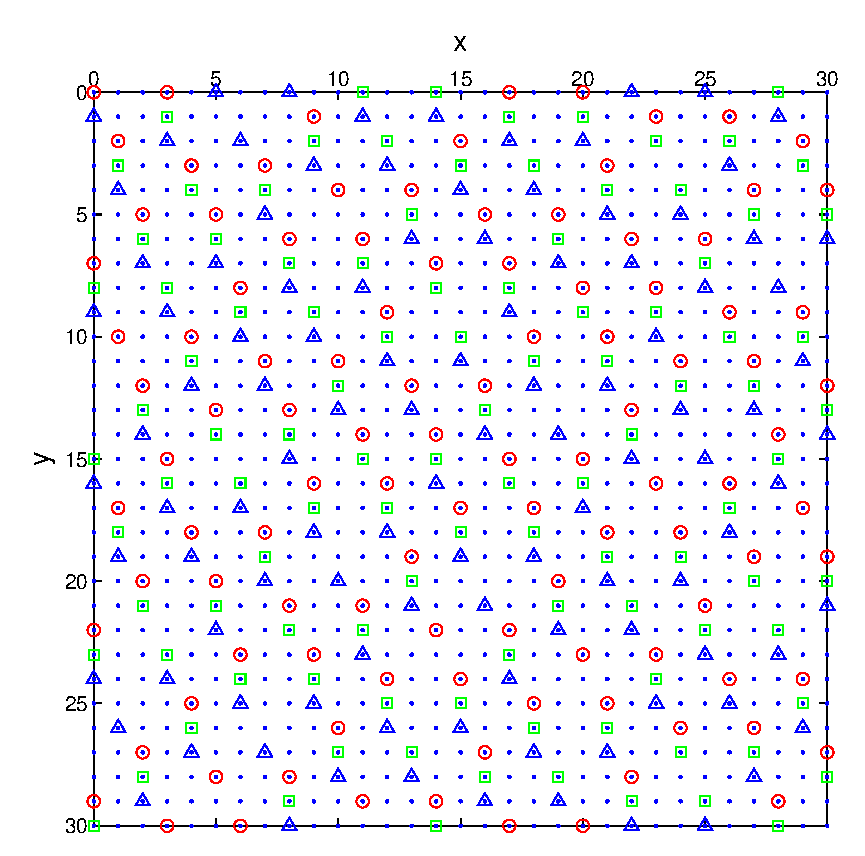
\includegraphics[width=7cm]{figure_sampling_view1.eps}
	%    \medskip
	%    \centerline{(a)}
	%  \end{minipage}\hfill
%  \begin{minipage}[t]{0.49\linewidth}\centering
	%    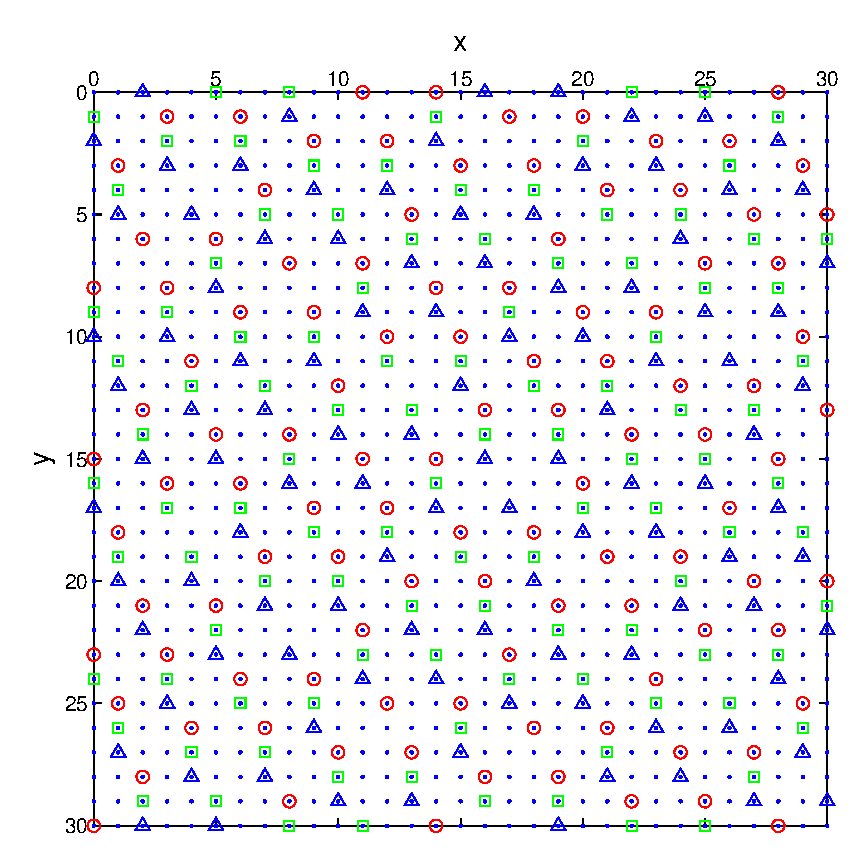
\includegraphics[width=7cm]{figure_sampling_view2.eps}
	%    \medskip
	%    \centerline{(b)}
	%  \end{minipage}
%  \caption{Assignment of single-view intensities to RGB components: (a) view
	%    \#1; and (b) view \#2. }
%  \label{fig:Sampling}
%\end{figure}
%
%In all likelihood, you will need to insert tables. See one example on the next page.
%\clearpage
%
%\begin{table}[h]
%	\caption{Absolute disparity error per pixel for the test data from
	%		Fig.~\ref{fig:Sampling} and different parameter values. In each experiment one
	%		parameter is adjusted while other parameters are unchanged.} 
%	\centering
%	\renewcommand{\arraystretch}{1.2}
%	\begin{minipage}[b]{0.30\linewidth}
	%		\centerline{$\eta=6000$, $\mu=2000$}\smallskip
	%		\centering
	%		\begin{tabular}{ccc}
		%			\hline
		%			$K$ & $u_1$ & $u_2$\\
		%			\hline
		%			3   & 0.52 &0.46\\
		%			7   & 0.47 &0.43\\
		%			10  & 0.35 &0.36\\
		%			12  & 0.37 &0.36\\
		%			\hline
		%		\end{tabular}
	%	\end{minipage}
%	%
%	\begin{minipage}[b]{0.34\linewidth}
	%		\centerline{$K=10$, $\mu=2000$}\smallskip
	%		\centering
	%		\begin{tabular}{ccc}
		%			\hline
		%			$\eta$ & $u_1$ & $u_2$\\
		%			\hline
		%			1000&0.54& 0.45\\
		%			3000&0.43& 0.40\\
		%			6000&0.35& 0.36\\
		%			9000&0.37& 0.37\\
		%			\hline
		%		\end{tabular}
	%	\end{minipage}
%	%
%	\begin{minipage}[b]{0.32\linewidth}
	%		\centerline{$K=10$, $\eta=6000$}\smallskip
	%		\centering
	%		\begin{tabular}{ccc}
		%			\hline
		%			$\mu$ & $u_1$ & $u_2$\\
		%			\hline
		%			100 &1.00&1.16\\
		%			1000&0.53&0.47\\
		%			2000&0.35&0.36\\
		%			3000&0.44&0.43\\
		%			\hline
		%		\end{tabular}
	%	\end{minipage}
%	%
%	\label{tab:Parameters}
%\end{table}

Of course, there must be a Table of Contents, List of Figures and List of Tables at the beginning of the thesis, but this is all set up automatically.

{\bf Important}: You will also be using a lot of citations. The format in this template follows the so-called APA style and looks as follows in the document body: \cite{lamport1985:latex}, \cite{Debr01}. There are no numbers in the list of references -- the list is sorted alphabetically according to the first author's last name.

Other styles of references are allowed by the library as well, e.g., ``plain'' or ``'ieee'', which use numbers in square brackets both in the document body and in the list of references. In order to use another style of references, e.g., ``plain'', follow the steps below:
%
\begin{enumerate}
	\item In ``thesis.tex'' file:
	\begin{itemize}
		\item comment out the line ``$\backslash$usepackage\{apalike\}'' at the top of the file,
		\item replace ``$\backslash$bibliographystyle\{apalike\}'' with ``$\backslash$bibliographystyle\{plain\}'' towards the bottom of the file.
	\end{itemize}
	\item In ``bu\_ece\_thesis.tex'' file, comment out all lines in the BIBLIOGRPAHY section (lines 503-517) and save it!
	\item Recompile ``thesis.tex'' twice
\end{enumerate}



\section{case study}

Gegeven is een IoT device dat al in gebruik is door maximaal 30 klanten. In dit onderzoek willen we voor deze klanten een IoT componenten implementeren in de firmware van het systeem. Het component dat de Bidirectionele communicatie van de ESP 32-chip verzorgd werkt aan de hand van de ESp-idf SDK. Alleen deze is geschikt voor implementatie in het huidige project.   



Het IoT device leest data uit de sensoren en formatteert deze data in een json string met behulp van de c-functie c-strcat(). De dataset wordt gepushed in JSON naar Thingsboard. Het data object bestaat uit de attributen vastgelegd in de tabel in de bijlage.
Datatransformate in de rulechain
https://thingsboard.io/docs/user-guide/rule-engine-2-0/tutorials/transform-incoming-telemetry/ 


Dataverwerking is relevant omdat er wordt verwerkt met verschillende type variabelen: BOOLEAN, INT, FLOAT en DOUBLE



\section{Onderzoeksvraag}

\begin{frame}[shrink=40]{Methoden}
	\begin{table}[htbp]
		\centering
		\begin{tabular}{|c|c|c|c|c|}\hline
			Index&Onderzoeksvraag&Onderwep&methode&Hiaat\\\hline
			5&\multicolumn{1}{m{2cm}|}{ }&\multicolumn{1}{m{3cm}|}{ Beschikbare platformen
				
			}&
			\multicolumn{1}{m{4cm}|}{ }&\multicolumn{1}{m{3cm}|}{ }\\\hline
			
			5&\multicolumn{1}{m{2cm}|}{ }&\multicolumn{1}{m{3cm}|}{Matrix Platform eigenschappen
				
			}&
			\multicolumn{1}{m{4cm}|}{ }&\multicolumn{1}{m{3cm}|}{ }\\\hline
			
			5&\multicolumn{1}{m{2cm}|}{ }&\multicolumn{1}{m{3cm}|}{ Feature selectie
				
			}&
			\multicolumn{1}{m{4cm}|}{ }&\multicolumn{1}{m{3cm}|}{ Achtergrondinformatie gekozen platform
				
			}\\\hline
			
			5&\multicolumn{1}{m{2cm}|}{ }&\multicolumn{1}{m{3cm}|}{Communicatie Protocol
				
			}&
			\multicolumn{1}{m{4cm}|}{ }&\multicolumn{1}{m{3cm}|}{ }\\\hline
			
			5&\multicolumn{1}{m{2cm}|}{ }&\multicolumn{1}{m{3cm}|}{Ontwerp
				
			}&
			\multicolumn{1}{m{4cm}|}{ }&\multicolumn{1}{m{3cm}|}{Bouw op minimaal 2 platformen een testopstelling (aansluiting, dataverwerking, visualisatie) 
				
			}\\\hline
			
			5&\multicolumn{1}{m{2cm}|}{ }&\multicolumn{1}{m{3cm}|}{ Testen 
				
			}&
			\multicolumn{1}{m{4cm}|}{ }&\multicolumn{1}{m{3cm}|}{ }\\\hline
			
			5&\multicolumn{1}{m{2cm}|}{ }&\multicolumn{1}{m{3cm}|}{ Realisatie
				
			}&
			\multicolumn{1}{m{4cm}|}{ }&\multicolumn{1}{m{3cm}|}{ }\\\hline
			
			
			
		\end{tabular}
	\end{table}
	
\end{frame}





\section{Inclusie en exclusiecriteria}
Dataverzameling platformen
Feature selectie
Kosten
rapporten/dissertaties over state nof the art, provisioning, RBAC, user management, MQTT, MQTT security, MQTTMessage service alternatives


Voor een onderzoek naar de metric voor het beoordelen van UI bouwmogelijkheden  is er een deskresearch gedaan naar de principes van dashboard design. Dit leverde geen bruikbare resultaten op. Daarom is samen met de opdrachtgever een brainstorm gedaan over de provisioning van het IoT device. De must haves zijn gespecificeerd per user interface


\section{referentie naar de onderzoeksmethoden}
Referenties naar de methode die gebruikt zijn in onderzoek inclusief de statistische methode

\section{identificatie}
Identificador de variabelen, datasets en route van administratie(hoe de gegevens zijn vastgelegd

\section{binding en randomisatie}
Methode van opschorting van errors, blinding, introductie van een controle groep zoals een placebo of randomisatie

\section{meetinstrument}
Het meetinstrument dat is gebruikt en de kwaliteiten daarvan uitgedrukt in betrouwbaarheid objectiviteit en precisie

\section{omschrijving dataverzameling}
Stap 1 zoeken io ioT cloud
vervolgens controleren op features als user management, mqtt connectoren, dashboard, white labeling
vervolgens open/closed source en locatie
vervolgens pricing categorien
Stap 2 data cleanup
- alle home automation/ smart home, home devices verwijderen
Stap 3
sdk onderzoeken, welke programmeertaal wordt er gebruikt 
Stap
welke documentatie is er beschikbaar
Stap
is het makkelijk aan te sluiten
Stap
Zijn er implementaties van beschikbaar voor de esp32

\paragraph{Betrwoubaarheid en validiteit}

\paragraph{data availability statement}

\section{setting waarin onderzoek plaatsvond}
Er is nog weinig bekend over de ontwikkelkosten voor een IoT cloud platform integratie. De verschillende platformen hebben verschillende prijsklassen en dat maakt de berekening complex. Omdat we in de beginfase zo min mogelijk kosten willen maken met een een makkelijk aansluitbaar systeem moet er uit de onderzoeksresultaten een oplossing komen voor een platform dat in de cloud werkt met de gewenste features maar dat ook makkelijk aan te sluiten is. Een voorbeeld is en proeflicentie waar we gedurende een jaar of enkele werken gebruik van kunnen maken en/of het project makkelijk over kunnen zetten.

\section{data analyse procedure}

\section{testomgeving}

\paragraph{software setup}



\paragraph{hardware setup}

 \newpage
\section{Requirementsengineering}

\subsection{Rampen}
 

\subsubsection{Mali}
Een granaat explodeerd in een mortier
De medische zorg na het ongeval was neit voldoende


De algemeen militair verpleegkundige gaf aan het slachtoffer nar het vn-hospitaal in kidal te brengen
De chaauffeur van de bushmaster kende de locatie niet  en bracht het slachtoffer naar een door frane militairren bemand hospitaal mmet minder mediswche faciliteiten
Hierna alsnog overgebracht naar het vn-hospitaal.
Dit verlieop  neit door nederlandse maatstaven.
pas toen een nederlandse arts arrivveerde werd door de Tongolese artsen een buikoperatie uitgevoerd.
Dit gebrurde zonder adequate anesthesie.
Na de operatie werde de gewonde militair overgelogen naar nederland. En later naar nederland.


granaat stond niet op scherp en in afgegaan in veilige stand
Granaat werd opgeslagen in neit gekoelde containers waardoor deze aan te hoge temeperaturen zijn blootgesteld.
Door de comvinatie van vocht en warmte in de granaat zeer gevoelige explosieve stoffen werden gevormd.
Tijdens de oefening was de fatale granaat in de zon.
Het afsluitplaatje in de granaat bleek niet in staat om doorslag in veilige stand te voorkomen waarna de granaat explodeerde.
De moritren zijn aangeschaft bij de amerikanen. gredurende de aanschafperiode zijn procedures en controles op kwaliteit en veiligheid deels nagelaten.
Dit veiligheidsgarantie werd vermeld in het koopcontract.
Conclusie
Koopcontract werd niet goed doorgelezen
Geen controle op kwaliteit en veiligheid
Geen controle op kwaliteit en veiligheid
Zwakke plekken in het ontwerp
Geen controle op kwaliteit en veiligheid
opslag en gebruik in ongunstige condities

De aanwezige medische voorzieningen waren nite volgends de nederlandse militaire richtlijnen
Het ontbreek aan medische toetsing vanuit de defensie organisatie
twijfels die werden geuit binnen de defensieorganisae vonden geen wrrklank
Ok het ongeval tijdens de mortieroefening was voor defensie geen aanleuiding om de medische voorzienignen te evalueren.
De inrichting van veilige medische zorg voor nederlandse militairen in kidal is ondergeschikt gemaakt aan de voortgang van de missie.


https://www.youtube.com/watch?v=PC2ekl4SaNA 

 
Een granaat explodeerd in een mortier
De medische zorg na het ongeval was neit voldoende


De algemeen militair verpleegkundige gaf aan het slachtoffer nar het vn-hospitaal in kidal te brengen
De chaauffeur van de bushmaster kende de locatie niet  en bracht het slachtoffer naar een door frane militairren bemand hospitaal mmet minder mediswche faciliteiten
Hierna alsnog overgebracht naar het vn-hospitaal.
Dit verlieop  neit door nederlandse maatstaven.
pas toen een nederlandse arts arrivveerde werd door de Tongolese artsen een buikoperatie uitgevoerd.
Dit gebrurde zonder adequate anesthesie.
Na de operatie werde de gewonde militair overgelogen naar nederland. En later naar nederland.


granaat stond niet op scherp en in afgegaan in veilige stand
Granaat werd opgeslagen in neit gekoelde containers waardoor deze aan te hoge temeperaturen zijn blootgesteld.
Door de comvinatie van vocht en warmte in de granaat zeer gevoelige explosieve stoffen werden gevormd.
Tijdens de oefening was de fatale granaat in de zon.
Het afsluitplaatje in de granaat bleek niet in staat om doorslag in veilige stand te voorkomen waarna de granaat explodeerde.
De moritren zijn aangeschaft bij de amerikanen. gredurende de aanschafperiode zijn procedures en controles op kwaliteit en veiligheid deels nagelaten.
Dit veiligheidsgarantie werd vermeld in het koopcontract.
Conclusie
Koopcontract werd niet goed doorgelezen
Geen controle op kwaliteit en veiligheid
Geen controle op kwaliteit en veiligheid
Zwakke plekken in het ontwerp
Geen controle op kwaliteit en veiligheid
opslag en gebruik in ongunstige condities

De aanwezige medische voorzieningen waren nite volgends de nederlandse militaire richtlijnen
Het ontbreek aan medische toetsing vanuit de defensie organisatie
twijfels die werden geuit binnen de defensieorganisae vonden geen wrrklank
Ok het ongeval tijdens de mortieroefening was voor defensie geen aanleuiding om de medische voorzienignen te evalueren.
De inrichting van veilige medische zorg voor nederlandse militairen in kidal is ondergeschikt gemaakt aan de voortgang van de missie.


https://www.youtube.com/watch?v=PC2ekl4SaNA 
\subsubsection{tesla crash report}
Door een softwarefout zijn er situaties ontstaan waarin het systeem informatie een onvoldoende informatie positie had om de juiste beslissingen te maken. Of dat de informatieverwerking niet juist was.
 


\subsubsection{ethiek}
 

\subsubsection{ cyber aanval op Oekraïene }


Hackers konden door het versturen van corrupte emails zichzeklf toegang verschaffen tot  SCADA controle systemen. Door de dienstdoende operators uitgebreid te observeren.
first doing reconnaissance to study the networks and siphon operator credentials, then launching a synchronized assault in a well-choreographed dance.
Ondanks dat de elektriciteitescentrale soms nog beter was beveiligd dan in de VS. toch is het de hackers gelukt door medewerkers logging remotely into the SCADA network, the Supervisory Control and Data Acquisition network that controlled the grid, weren't required to use two-factor authentication, which allowed the attackers to hijack their credentials and gain crucial access to systems that controlled the breakers.
%https://en.wikipedia.org/wiki/Ukraine_power_grid_hack 


 


\subsubsection{schipholbrand}
 



\subsubsection{therac-25}
Softwarefout uit zich als hardwarefout de klachtafhandeling geen onderzoek geen second opinion is prioriteit wel 
gechecked na onderzoek bellen en geen prioriteit aanwezig te zijn alleen importeurs en fabriken mogen fouten 
in frabrieksinstellingen rapporteren 
Therac25 Systeem ligt plat veel voorkomende eror stdaardafhandeling om de error te verwerpen resultaat: 
de patient kreeg overdosis patient overleden onderzoek opgestart, stuatie niet reproduceerbar foutmarkering: 
gezien als uitzonderlijk, software aanpassing van groote magnitude 5; de oorzaak was waarschijlijk mechanisch 
maar neit vastgesteld; conceptueel odel niet aangepast probleemclassicificatie door autorititen het probleem 
en de impact daarvan anar beneden bijgesteld AEFL doe gedeeltelijke aanpassing om hardware na berisping 
Canadese autoriteit 
Derde patient overleden door eythema AECL wijst alle doodsoorzaken af AECL beweert dat geen vergeli- 
jkbare voorvalle bij andere machines of patienten zijn voorgekomen geen vervolgonderzoek vanwege garanties 
bedrijf gaat uit van geen mogelijke functionele fout 
vierde patient overleden aan overdodis ontstaan door bug in software onjuiste aanduiding bij de foutmelding 
verkeerde reactie/invoer ddoor operator communicatie tussen patient en operator werd onvoldoende gemon- 
itorred ( apparatuur niet aangesloten, en audio monitor kapot) engineer van AECL stelt geen fouten vast 
Engineer AECl kan fout niet reproduceren Geen communicate tussen bedrijf en uitgezonden technisci over 
vergelijkbare probleemgevallen 
vijfde geval malfunction 54 leidt tot overdosis en de dood fout gereproduceerd door operator bedrijf fout 
was daa entryspeed herpublicatie van de ongevallen en de eerdere ongevallen in de meia apparaat wel nog in 
gebruik genomen niet handig, waarschuwingsberichten en aanwijzingen voor een bugfix naar de gebruikers door 
druk van fda is bedrijf op zoek gegaan naar permanente oplossing 
zesde geval software fout door softwarefout otntstaat lightstruct .. op de patient na onderzoek door AECL 
blijkt niet alleen hardware de oorzak gebruikers direct geinformeerd oplossing gevonden, media ingeschakeld om 

transparantie af te dwingen door de gebruikersgroep en de FDA AECL gedwongen functionaliteit aan te passen 
Engineers hebben meer studie moeten maken van gebruikte technologie en onderhoudbaarheid daarvan 


\subsubsection{Ramp schietpartij militair ossendrecht }
Een militaire overleid op een schietbaan in ossendracht door onvoldoende begeleiding van cursisten, geen toezicht op de lokatie. E\r was een instructuur in opleiding die niet volledig was mmeegenomen in het poroces en ook was er geen baancommandant aanwezig. Geen van de aanwezig instructeurts had de juiste papieren om de cursisten te begeleiden. De aanwezig instruceur had geen zich op de instructeur in opleiding, evenmin de andere militairen. In de instructiehandleiding ontbreken richtlijnen voor bijzondere schietbanen. Ook was er geen keuring. Door personelstekort is er geen andacht besteed aan documentastie(een slyllabus) hoe en met welke risico’s oefeningnen moeten worden ingericht. Ok werd er vooraf geen veiliheidsanaklyse gedaan. Het gebrek aan lesmateriaal en deskundigen is gemeld binnen de defensieorganisatie maar dit heeft niet geleid tot enige verandering in de situatie.
Op een afgekeurde scheitbaan
Tezicht door een instructeur in opleiding die zelf geen persoonlijke begeleiding heeft gehad tijdens de uitvoering
Belangrijk is dat defensie haar taken kan uitvoeren met personeel dat is getraind in situaties die de risicos van de werkomgeving aan de cursisten kunnen laten zien.
Conclusie
Zonder gekwalificeerde instructuers.
Zonder toezicht
Zonder lesmateriaal
Zonder adequate veiligheidsanalyse
https://www.youtube.com/watch?v=6jmkDClGDHo 


\subsubsection{molukse treinkaping }
https://www.youtube.com/watch?v=h99Fe9XzzHI 

\subsubsection{vuurwerkramp in enschede }
https://www.enschede.nl/inhoud/commissie-oosting 
https://www.politie.nl/binaries/content/assets/politie/wob/00-landelijk/vuurwerkramp-enschede/bijlagen-rapport-vuurwerkramp-enschede.pdf 
https://www.researchgate.net/publication/254815008_Rampen_regels_richtlijnen 

 





\subsubsection{explosie in libabon, beirut 
}

Op 23 september 2013 voer het vrachtschip de Rhosus onder Moldavische vlag[7] van Batoemi in Georgië naar Beira in Mozambique met 2.750 ton ammoniumnitraat

Gezien het ernstige gevaar van het bewaren van deze goederen in de hangar onder ongeschikte klimatologische omstandigheden, herhalen we ons verzoek aan de marine-instantie om deze goederen onmiddellijk weer te exporteren om de veiligheid van de haven en de mensen die er werken te verzekeren, of om akkoord te gaan om ze te verkopen.
Voorafgaand aan de explosie was er een brand in een opslagplaats. 

https://www.hrw.org/report/2021/08/03/they-killed-us-inside/investigation-august-4-beirut-blast 
https://www.researchgate.net/publication/348325979_Beirut_Explosion_the_full_story 
https://reliefweb.int/sites/reliefweb.int/files/resources/CaseStudy_BeirutExplosion_TechBioHazardsweb.pdf 
\subsubsection{explosie tanjin china 
}

Later bleek uit een onderzoek van de Chinese autoriteiten dat de explosie overeenkwam met de ontploffing van 450 ton TNT.[6] 
De oorzaak van de explosie lag in de spontane zelfontbranding van 207 ton cellulosenitraat dat in containers was opgeslagen op het terminalterrein.[6] 
Verder lag op een tweede locatie nog eens 26 ton van dit explosieve materiaal opgeslagen.
De tweede ontploffing werd versterkt door de opslag van 800 ton kunstmest in de vorm van ammoniumnitraat in de nabijheid.[6]
De opslag van cellulosenitraat is aan strenge regels gebonden. Het moet koel en droog worden opgeslagen. De containers stonden buiten opgesteld in de brandende zon. De temperatuur liep op tot 36 °C en bereikte binnen de containers waarschijnlijk de 65 °C.[6] De verpakking van de cellulosenitraat droogde uit waardoor de ontploffing kon ontstaan. Op het terrein lagen meer gevaarlijke stoffen opgeslagen dan waarvoor vergunningen waren verstrekt.[6] Dit leidde tot een kettingreactie met grote schade tot gevolg. Door de brand en bluswater is in de directe omgeving veel milieuschade opgetreden.


https://www.hindawi.com/journals/joph/2019/1360805/ 

\subsubsection{bijlmerramp}
Motor 3 (de binnenste motor aan de rechtervleugel van het vliegtuig) brak af, beschadigde de vleugelkleppen en botste tegen motor 4 die vervolgens ook afbrak.
De ernst van de situatie werd op Schiphol niet goed ingezien. Dit kwam onder meer doordat lost in de luchtvaart de gebruikelijke term is om het verlies van motorvermogen te melden. Op Schiphol werd er dan ook van uitgegaan dat er twee motoren waren uitgevallen. Dat ze letterlijk verloren waren wist men niet. Gezien het grote aantal handelingen dat de bemanning in een paar minuten moest uitvoeren en de keuzes die de piloot maakte, veronderstelde de parlementaire enquêtecommissie die de ramp later zou onderzoeken dat ook de bemanning waarschijnlijk niet heeft geweten dat beide motoren van de rechtervleugel waren afgebroken. De buitenste motor van een 747 is vanuit de cockpit slechts met moeite zichtbaar en de binnenste motor helemaal niet.

Op de avond van de 4e oktober 1992 was landingsbaan 06 (de Kaagbaan) in gebruik. De piloot verzocht de luchtverkeersleiding op Schiphol echter een noodlanding te mogen maken op de Buitenveldertbaan (baan 27). Waarom hij juist deze baan koos, is nooit duidelijk geworden. Een keuze voor deze baan lag niet voor de hand; omdat de wind uit het noordoosten kwam, zou het toestel met flinke staartwind moeten landen. Langs de landingsbaan waren enkele grote brandweerwagens van Schiphol geplaatst. Deze zogeheten crashtenders moesten een brand tijdens de landing meteen blussen. Na de crash werd één zwarte doos teruggevonden. De bijbehorende band was in vier stukken gebroken, waardoor de laatste 2 minuten en 45 seconden ervan niet meer te gebruiken waren. De doos werd voor onderzoek naar Washington gestuurd en leverde uiteindelijk onderstaande informatie op.
Om goed uit te komen voor de landingsbaan vloog het beschadigde toestel eerst nog een rondje boven Amsterdam. Tijdens dit rondje gaf de gezagvoerder de copiloot opdracht de vleugelkleppen (flaps) uit te schuiven. Links schoven de kleppen uit, maar doordat de afgebroken motor 3 de rechtervleugel had beschadigd schoven de kleppen op die vleugel niet uit. Als gevolg hiervan kreeg het toestel links meer draagvermogen dan rechts. De piloot meldde aan de verkeersleiding dat er ook problemen met de flaps waren.
Aanvankelijk ging het aanvliegen van de Buitenveldertbaan goed. Op het moment dat het vliegtuig daalde tot onder de 1500 voet en snelheid minderde, raakte het echter compleet onbestuurbaar en maakte het een ongecontroleerde, scherpe bocht naar rechts. Over de radio was te horen dat de gezagvoerder zijn copiloot in het Hebreeuws opdracht gaf om alle kleppen in te trekken en het landingsgestel uit te klappen. Vervolgens meldde de copiloot in het Engels aan de luchtverkeersleider dat het toestel zou gaan neerstorten. Uit later onderzoek bleek dat het vliegtuig eerder enkel recht bleef vanwege de hoge snelheid (280 knopen, zijnde 519 km/u). Doordat de rechtervleugel beschadigd was, was het moeilijker om het vliegtuig recht te houden. Alleen de hoge snelheid zorgde ervoor dat er nog voldoende draagvermogen was. Toen bij het inzetten van de landing de snelheid verlaagd werd, werd het draagvermogen van de rechtervleugel echter dusdanig gering dat het toestel niet meer onder controle te houden was en een duikvlucht naar rechts maakte.

https://aviation-safety.net/database/record.php?id=19921004-2&lang=nl 


\subsubsection{slmramp}
Toen de Anthony Nesty Zanderij naderde, was het daar, anders dan het weerbericht had voorspeld, mistig. Het zicht was evenwel niet zo slecht dat er niet op zicht kon worden geland. Gezagvoerder Will Rogers besloot echter via het Instrument Landing System (ILS) te landen, hoewel dit niet betrouwbaar was en hij voor zo'n landing ook geen toestemming had. De gezagvoerder brak drie landingspogingen af. Bij de vierde poging negeerde de bemanning de automatische waarschuwing (GPWS) dat het toestel te laag vloog. Het toestel raakte op 25 meter hoogte twee bomen. Het rolde om de lengteas en stortte om 04.27 uur plaatselijke tijd ondersteboven neer.

Uit onderzoek bleek dat de papieren van de bemanning niet in orde waren. 
Geconcludeerd werd dat de gezagvoerder roekeloos had gehandeld door voor een ILS-landing te kiezen terwijl hij daar geen toestemming voor had, en door onvoldoende op de vlieghoogte te hebben gelet. 
De SLM werd verweten de kwalificaties van de bemanning onvoldoende te hebben gecontroleerd.

https://aviation-safety.net/investigation/cvr/transcripts/cvr_py764.php 
https://aviation-safety.net/database/record.php?id=19890607-2 

\subsubsection{ethiopian airlines}
Ethiopian Airlines Flight 302
Door problemen met de flight control
One minute into the flight, the first officer, acting on the instructions of the captain, reported a "flight control" problem to the control tower.
Two minutes into the flight, the plane's MCAS system activated, pitching the plane into a dive toward the ground. The pilots struggled to control it and managed to prevent the nose from diving further, but the plane continued to lose altitude.
The MCAS then activated again, dropping the nose even further down. The pilots then flipped a pair of switches to disable the electrical trim tab system, which also disabled the MCAS software. However, in shutting off the electrical trim system, they also shut off their ability to trim the stabilizer into a neutral position with the electrical switch located on their yokes. The only other possible way to move the stabilizer would be by cranking the wheel by hand, but because the stabilizer was located opposite to the elevator, strong aerodynamic forces were pushing on it.
As the pilots had inadvertently left the engines on full takeoff power, which caused the plane to accelerate at high speed, there was further pressure on the stabilizer. The pilots' attempts to manually crank the stabilizer back into position failed.
Three minutes into the flight, with the aircraft continuing to lose altitude and accelerating beyond its safety limits, the captain instructed the first officer to request permission from air traffic control to return to the airport. Permission was granted, and the air traffic controllers diverted other approaching flights. Following instructions from air traffic control, they turned the aircraft to the east, and it rolled to the right. The right wing came to point down as the turn steepened.
At 8:43, having struggled to keep the plane's nose from diving further by manually pulling the yoke, the captain asked the first officer to help him, and turned the electrical trim tab system back on in the hope that it would allow him to put the stabilizer back into neutral trim. However, in turning the trim system back on, he also reactivated the MCAS system, which pushed the nose further down. The captain and first officer attempted to raise the nose by manually pulling their yokes, but the aircraft continued to plunge toward the ground.

https://www.hindawi.com/journals/ijae/2014/472395/ 


\subsubsection{stint ongeluk}
Vier kinderen, een bestuurder kwamen om en een vijfde persoon , een kind raakte zwaargewond. Uit odnerzoek van bleek :
Foute torsieveer voor de gashendel werd geleverd
Geen van de drie onderzochte voertuigen haalden de wettelijk vereiste remvertraging
De automatische parkeerrem kan leiden tot gevaarlijke situaties wanneer deze ongewenst geactiveerd wordt tijdens het rijden. 
Het losraken van de nuldraad naar de gashendel leidt volgens TNO tot ongewenst versnellen van het voertuig en een oncontroleerbare situatie voor de bestuurder.
Voor alle drie onderzochte voertuigen geldt dat het ontbreken van een zitplaats leidt tot veiligheidsrisico’s voor remmen en sturen door de grotere kans dat de bestuurder van het voertuig valt. Als de bestuurder van een Stint valt, leidt dit in alle rijsituaties tot een onbeheersbare situatie


https://repository.tno.nl/islandora/object/uuid%3Acdef48df-da49-46b6-8678-5c62a88a0090 


\subsubsection{tjernobyl}
Een ramp bij een kernreacor in de sovjetunie. Door een bedieningsfout in een testprocedure werd het vermogen van de koelinstallaties negatief beinvloed. Door een ontwerpfout in de noodstopprocedure kon in het systeem niet snel genoeg schakelen om remmende invloed uit te oefenen op het toenemende vermogen van de reactorkernen. Met brand en eksplosie tot gevolg.
https://www-pub.iaea.org/MTCD/publications/PDF/Pub913e_web.pdf 

\subsubsection{ecounrt in de nerderlandse rechdspraak}
https://www.njb.nl/blogs/a-court-with-no-face-and-no-place/ 
http://www.e-court.nl/wp-content/uploads/2018/03/Procesreglement-e-Court-2017_20180201.pdf 


 

\subsubsection{ramp turkisch airlines}
Inadequaat handelen van de piloten ondanks een defecte hoogtemeter en onvolledige instructies van de luchtverkeersleiding/
https://catsr.vse.gmu.edu/SYST460/TA1951_AccidentReport.pdf 

Wat ging er allemaal mis bij de bovengenoemde rampen en ongelukken....... 

Wat hebben deze rampten te maken met de requirements en specificaties van deze odpracht? 


\subsubsection{automatisering van waterwerken}
https://hbo-kennisbank.nl/searchresult?q=sluizen 
artificial inte;lligence and water locks 
https://www.sciencedirect.com/science/article/pii/S0160791X21002165 
https://www.wwdmag.com/artificial-intelligence/sewer-monitoring-turns-ai 
https://www.anylogic.com/resources/articles/analysis-of-the-expansion-of-the-panama-canal-using-simulation-modeling-and-artificial-intelligence/ 
ai used in public infrastructure thesis 
https://blog.ferrovial.com/en/2020/10/how-artificial-intelligence-is-used-for-infrastructure-maintenance/ 
https://www.tilburguniversity.edu/about/schools/law/departments/plg/ai-public-sector 
artificaial used in water shipping 
artificial used in maritime transport 
artificaial used in water shipping 
ai used in maritime traffic 



https://www.ftm.nl/artikelen/waternet-verantwoordelijkheid-digitaal-wanbeleid 
https://open.overheid.nl/repository/ronl-bc28f344-af87-481a-aea6-58c481b4cdc8/1/pdf/ilt-onderzoeksrapport-stichting-waternet.pdf\ 
https://www.security.nl/posting/697815/Waternet+onder+verscherpt+toezicht+wegens+onvoldoende+grip+op+cybersecurity 
https://www.security.nl/posting/677368/Inspectie+doet+onderzoek+naar+Waternet+na+verzwegen+penetratietest 
https://www.parool.nl/nederland/onderzoeksraad-rijk-houdt-informatie-over-cyberveiligheid-achter-met-grote-risico-s~b673ec1f/?referrer=https%3A%2F%2Fwww.google.com%2F 


google: artiifcial intelligence for industrial control systems researchgate 
https://link.springer.com/chapter/10.1007/978-3-030-38557-6_7 
automation  for industrial control systems 
researchgate 
google scholar:automation of industrial control systems problems 
hindawi.com: problems industrial control systems 

\subsubsection{Artificial intelligence en water locks}
 

\subsection{ethiek}

 
Ethiek 



persuasive technology 
https://www.humanetech.com/youth/persuasive-technology 
https://www.minddistrict.com/blog/persuasive-technology-new-insights-in-behavioural-change 
https://www.sciencedirect.com/book/9781558606432/persuasive-technology 
https://spectrum.ieee.org/how-persuasive-technology-can-change-your-habits 
https://www.frontiersin.org/articles/10.3389/frai.2020.00007/full 
https://psmag.com/environment/captology-fogg-invisible-manipulative-power-persuasive-technology-81301 
https://www.makeuseof.com/what-is-persuasive-technology/ 
https://lib.ugent.be/catalog/rug01:001235489 
https://cyberpsychology.eu/article/view/12270 


\subsubsection{mode confusion }
Mode confusion treed op als geobserveerd gedrag van een technisch systeem niet past in het gedragspatroon 
dat de gebruiker in zijn beeldvorming heeft en ook niet met voorstellingsvermogen kan bevatten 


\subsection{Een goed model}

What is a Good Model?
To some extent, building good models is an art. Dijkstra's motto "Beauty is our business" applies to models as well as to programs. Nevertheless, we can state seven criteria for good models. These criteria are in some sense obvious, and any person with experience in modelling will often try to adhere to them. But surprisingly, our list of criteria has - to the best of our knowledge - not been described elsewhere in the literature, although most of them occur in a technical report of Mader, Wupper and Boon. (We see this as a clear indication of the lack of interest for the methodology of modeling in our field.) Often, the criteria are hard to meet and typically several of them are conflicting. In practice, a good model is often one which constitutes the best possible compromise, given the current state-of-the-art of tools for modelling and analysis. But a truly beautiful model meets all the criteria! We refer to Mader, Wupper and Boon for further links to related work in the areas of software engineering, requirements analysis, and design.
\paragraph{Specification}
A good model has a clearly specified object of modelling, that is, it is clear what thing the model describes. The object of modelling can be (a part of) an existing artefact or physical system, but it may also be a document that informally specifies a system or class of systems (for instance a protocol standard), and it may even be a collection of ideas of a design team about a system they construct, expressed orally and/or by some drawings on a whiteboard.
A good model has a clearly specified purpose and (ideally) contributes to the realization of that purpose. Possible purposes include: communication between stake holders, verification of specific properties (safety, liveness, timing,..), analysis and design space exploration, code generation, and test generation. A model can be descriptive or prescriptive. If a model has to serve several distinct purposes then often it is better to construct multiple models rather than one.
\paragraph{Traceable}
A good model is traceable: each structural element of a model either (1) corresponds to an aspect of the object of modelling, or (2) encodes some implicit domain knowledge, or (3) encodes some additional assumption. Additional assumptions are for instance required when a protocol s tandard is incomplete (e.g., it does not specify how to handle certain events in certain cases). Links between the structural elements of the model and the aspects of the object of modelling should be clearly documented. A distinction must always be made between properties of (a component of) a model and assumptions about the behavior of its environment.
\paragraph{Truthfullnes}
A good model is truthful: relevant properties of the model should also carry over to (hold for) the object of modelling. Typically, for each (relevant) behavior of the object of modelling there should be a corresponding behavior of the model, and/or for each behavior of the model there should be a corresponding behavior of the artefact. In the construction of models often idealizations or simplifications are necessary in order to allow for the use of a certain modeling formalism or in order to be able to analyze the model. In these cases, the model may not be entirely truthful. The modeller should always be explicit about such idealizations/simplifications, and have an argument why the properties of the idealized model still say something about the artefact. In the case of quantitative models this argument will typically involve some error margin. In the case of nondeterministic models it frequently occurs that a model ``overapproximates'' reality, and that certain behaviors that are possible in the model are not possible for the artefact.
\paragraph{Simplicity}
A good model is simple (but not too simple). Occam's razor is a principle particularly relevant to modelling: among models with roughly equal predictive power, the simplest one is the most desirable. Hence, the number of states and state variables should be as small as possible, and the level of atomicity of transitions should be as coarse grained as possible (but not coarser), i.e., the number of transitions should be minimal given the intended use of the model. Preferably, things should be written only once, and one should avoid ugly encodings. Preferably, the model uses stable, well-defined and well-understood concepts and semantics.
A good model is extensible and reusable, that is, it has been designed to evolve and be used beyond its original purpose. Typically, if one defines models in a modular and parametric way this allows for dimensioning, future extensions and modifications, especially if modules have well-defined interfaces. Ideally, a model should not just describe the specific system at hand: by appropriate instantiation and dimensioning it should be possible to model a whole class of similar systems.
\paragraph{intgeroperability}
A good model has been designed and encoded for interoperability and sharing of semantics. Model-driven development of an embedded system typically leads to a plethora of models, all presenting different views on and abstractions of the system. If a model is not somehow linked to other models, its usefulness will be limited. Ideally therefore, the relationships between all models should be properly defined, for instance via formal refinement relations.
Clearly, there are many relationships and dependencies between the criteria. If a model is traceble, that is, links between the structural elements of the model and the aspects of the object of modelling are clearly documented, then chances increase that the model will be thrutful. Also, if a model has been set up in a modular way, then one may apply a divide-and-conquer strategy both for establishing truthfulness of the model and for analysis. Etc, etc.

Last change made on 23/2/2010. Please send comments to Frits Vaandrager


http://www.cs.ru.nl/~fvaan/PV/what_is_a_good_model.html


artiekelen

Programming languages and energy efficiency’
Preliminary MW and MMW Reflection and Transmission Measurements of a Silicon Wafer under Illumination of Light for Reflected Phased Array Antennas
Looking at Hands in Autonomous Vehicles: A ConvNet Approach using Part Affinity Fields
Security of the Internet of Things: Vulnerabilities, Attacks and Countermeasures
Active Scan-Beam Reflectarray Antenna Loaded with Tunable Capacitator
\subsection{Requirements}

Om een goed verhaal op te stellen, moet vooraf aan enkele voorwaarden
worden voldaan. De eerste voorwaarde is de geschiktheid van het
afstudeerproject. Als een afstudeerproject niet tot keuzes leidt, kan
men zich afvragen of dat wel een echte afstudeeropdracht is. Een
afstudeerproject zonder onderzoeksaspecten is ook verdacht. Daarnaast
moet een afstudeerproject passen in het profiel van een opleiding om
beoordeelbaar te zijn. De andere voorwaarde voor goed een verhaal is
de registratie van werkzaamheden tijdens het a
\subsection{specificaties}

Om een goed verhaal op te stellen, moet vooraf aan enkele voorwaarden
worden voldaan. De eerste voorwaarde is de geschiktheid van het
afstudeerproject. Als een afstudeerproject niet tot keuzes leidt, kan
men zich afvragen of dat wel een echte afstudeeropdracht is. Een
afstudeerproject zonder onderzoeksaspecten is ook verdacht. Daarnaast
moet een afstudeerproject passen in het profiel van een opleiding om
beoordeelbaar te zijn. De andere voorwaarde voor goed een verhaal is
de registratie van werkzaamheden tijdens het a
\subsection{Het vier variabelen model}

Systemen (met daarin software) en de bijbehorende vier variabelen:
Monitored variabelen: door sensoren gekwanticeerde
fenomenen uit de omgeving
Controlled variabelen: door actuatoren \bestuurde"
fenomenen uit de omgeving
Input variabelen: data die de software als input gebruikt
Output variabelen: data die de software levert als output

\subsubsection{Monitored variabelen}

Om een goed verhaal op te stellen, moet vooraf aan enkele voorwaarden
worden voldaan. De eerste voorwaarde is de geschiktheid van het
afstudeerproject. Als een afstudeerproject niet tot keuzes leidt, kan
men zich afvragen of dat wel een echte afstudeeropdracht is. Een
afstudeerproject zonder onderzoeksaspecten is ook verdacht. Daarnaast
moet een afstudeerproject passen in het profiel van een opleiding om
beoordeelbaar te zijn. De andere voorwaarde voor goed een verhaal is
de registratie van werkzaamheden tijdens het a
\subsubsection{Controlled variabelen}

Om een goed verhaal op te stellen, moet vooraf aan enkele voorwaarden
worden voldaan. De eerste voorwaarde is de geschiktheid van het
afstudeerproject. Als een afstudeerproject niet tot keuzes leidt, kan
men zich afvragen of dat wel een echte afstudeeropdracht is. Een
afstudeerproject zonder onderzoeksaspecten is ook verdacht. Daarnaast
moet een afstudeerproject passen in het profiel van een opleiding om
beoordeelbaar te zijn. De andere voorwaarde voor goed een verhaal is
de registratie van werkzaamheden tijdens het a
\subsubsection{Input variabelen}

Om een goed verhaal op te stellen, moet vooraf aan enkele voorwaarden
worden voldaan. De eerste voorwaarde is de geschiktheid van het
afstudeerproject. Als een afstudeerproject niet tot keuzes leidt, kan
men zich afvragen of dat wel een echte afstudeeropdracht is. Een
afstudeerproject zonder onderzoeksaspecten is ook verdacht. Daarnaast
moet een afstudeerproject passen in het profiel van een opleiding om
beoordeelbaar te zijn. De andere voorwaarde voor goed een verhaal is
de registratie van werkzaamheden tijdens het a
\subsubsection{Output variabelen}

Om een goed verhaal op te stellen, moet vooraf aan enkele voorwaarden
worden voldaan. De eerste voorwaarde is de geschiktheid van het
afstudeerproject. Als een afstudeerproject niet tot keuzes leidt, kan
men zich afvragen of dat wel een echte afstudeeropdracht is. Een
afstudeerproject zonder onderzoeksaspecten is ook verdacht. Daarnaast
moet een afstudeerproject passen in het profiel van een opleiding om
beoordeelbaar te zijn. De andere voorwaarde voor goed een verhaal is
de registratie van werkzaamheden tijdens het a


\subsection{Specificaties}

Voor alle paden geldt als een schip vertrekt is de sluisdeur dicht. 
Voor alle paden geldt als stoplicht op rood, sluisdeuren dicht 
Is een schip vertrokken dan is de nivelleermachine uit. 
Er is geen pad waarvoor geldt dat een schip vertrekt vanuit de rechtersluisdeur en de linkersluisdeur is open, linkeruitvaartstoplich en de linkerinvaarstoplicht op groen en nivelleermachine is aan. 
Er is een pad waarvoor geldt dat de linkersluisdeur dicht is, de rechtersluisdeur dicht is, de linkerinvaarstoplicht is gelijk aan rood, linkeruitvaarstoploicht is op rood en rechteruitvaarstoplicht is op rood en rechterinvaarstoplicht op rood terwijl er geen schip in de sluis ligt. 

Geen deadlock 
• Voor geen enkel pad geldt dat als de deuren gesloten zijn volgens de kluis dat er een deur openstaat om 
een schip naar buiten te laten. 
• Voor alle paden geld dat als een sluis aan het voorbereiden is, dan zijn alle duren dcht. 
• Voor alle paden geld dat als een deur dicht is het aantal schepen in de kade gelijk is aan nul 
• Voor een enkel pad geld dat als het binnenstoplicht op groen staat dat het niet toegestaan in naar binnen 
te varen 
• Voor alle paden geldt dat de globale tijd langer is dan 30 tijdseenheden 
• Er is een pad waarvoor geld dat als een schip wilt stoppen dat er meer dan 5 schepen in de sluis zitten. 
• Voor alle paden geldt als schip vrtrekt is sluisdeur dicht 
• Voor alle paden geldt als stoplicht op rood sluisdeuren dicht en schip vertrollen dan is de nivelleermachine 
uit 
• Er is geen pad waarop een schip vertrekt vanuit de rechtersluisdeur en de linkersluisdeur is open en 
linkeruitaartstoplicht en linkeruitvaartsoplicht opgroen en nibelleermachine is aan 
• Er is een pad waarvoor geldt dat linkerslsuisdeuren dicht zijn, rechtersluisdeuren dicht zijn rechteruit- 
vaartstoplicht is rood en rechteruitvaartstoplicht is rood terwijl eer geen schip in de sluis licht 
• EEn stopluch staat altijd op groen als de deuren open staan en de pomp niet bezig is. 
• In geen enkele staat van de sluis behalve tussen de lowergate en uppergate en uppergate en lowergate en 
de staten AtArrivalLow en AtEnteringHigh is de wachttijd langer dan 5 tijdseenheden 
• Voor alle paden in een pomp geldt dat als water level lager is dan waterlaag pompwaterweg is altijd false 
• Voor alle paden gelft dat als water level hoger is dan waterhoog dan is pompwater altjd false 
• Het zal nooit gebeuren dat een pomp water toevoegt als deuren open zjn, geen schip in sluis en stoplicht 
op groen 
• Het kan gebeuren dat bij pompr het stoplicht op rood staat, het schip in de sluis en deur is dicht, en 
waterstand gelijk aan waterlaag 
• Er is een mogelijkheid dat vanuit pomp get stoplicht op rood wordt gezet en waterlevel gelijk is aan 
waterlaag 
• Het kan voorkomen dat bij state pompaan het waterniveau gelijk is aan waterlaag 
• Voor alle paden gelt dat er een mogelijkheid is dat deur is open/dicht en sluis nivelleert omhoog/omlaag 
14 




Kripke strucuten


De set van initiele staten

De transities tussen de states

De state labeling fuctie voor elke state met een set van atomischr proosities die waar zijn voor een state

Met D ={0,1};
S = D*D
S0 = {(1,1)}
R=
L
  
\section{Requirementanalyse}

\subsection{Inleiding}
Een requirement is een opdracht gedefineerd door een klant. In requirement komt naar voren wat er specifiek wordt gevaard, voor wie het is bedoeld, of het meetbaar is,  de acceptatieeisen,een realistische perceptie  het doel of gewenst resultaat en binnen welke tijdseenheden het moet worden gerealiseerd.
 



\paragraaf{Algoritmen en broncode\cite{wikibooks}}

note={\url{http://...}}

\paragraaf{Algoritmen en broncode\cite{wikibooks}}

 
\subsection{Protocolllen}
Aan de hand van het onderzoek naar de verschillende cloud platformen is er een inzicht gekomen in de functionaliteiten van de applicaties. Enkele veelvoorkomende features die in overeenstemming zijn met de functionele eisen een lijst met platform features


\subsubsection{Vergelijking en Analyse}

\url{https://pure.tue.nl/ws/portalfiles/portal/46946084/855778-1.pdf}
\begin{frame}{Protocollen}
	\begin{table}[htbp]
		\centering
		\begin{tabular}{|c|c|c|c|}\hline
			Property&MQTT&COAP&LwM2M \cite{wikibooks}\cite{wikibooks} \\\hline
			
			
			
			Sterke punten &\multicolumn{1}{m{2cm}|}{}&\multicolumn{1}{m{4cm}|}{}&
			\multicolumn{1}{m{4cm}|}{ }\\\hline
			
			Sterke punten &\multicolumn{1}{m{2cm}|}{ }&\multicolumn{1}{m{4cm}|}{}&
			\multicolumn{1}{m{4cm}|}{ }\\\hline
			
			
			
		\end{tabular}
	\end{table}
	
\end{frame}

\subsection{categorisatie}
Aan de hand van het onderzoek naar de verschillende cloud platformen is er een inzicht gekomen in de functionaliteiten van de applicaties. Enkele veelvoorkomende features die in overeenstemming zijn met de functionele eisen een lijst met platform features

\footnote{Een pdf-bestand kan zowel vector-graphics als
	bitmap-graphics bevatten.}


\paragraaf{Algoritmen en broncode\cite{wikibooks}}

note={\url{http://...}}

\paragraaf{Algoritmen en broncode\cite{wikibooks}}
 


\subsection{analyse}


\subsubsection{Voor en nadelen analyse}

\paragraph{Handmatig}
\begin{enumerate}
	\item PROS
	\begin{enumerate}
		\item
	\end{enumerate}
	\item CONS
	\begin{enumerate}
		\item
	\end{enumerate}
\end{enumerate}

\paragraph{Automatisch}
\begin{enumerate}
	\item PROS
	\begin{enumerate}
		\item
	\end{enumerate}
	\item CONS
	\begin{enumerate}
		\item
	\end{enumerate}
\end{enumerate}
 



\subsubsection{IoT Security}
IoT security is a serious concern, but it’s not an impossible feat. Many emerging processes and policies around privacy are affecting IoT.
“There are a lot of standardizations around privacy regulation that can impact IoT for the better,” says Pat Wilbur, chief technology officer at Hologram. “That’s because security often comes as a consequence of privacy.”
However, there aren’t official standards to govern IoT security (yet), so it’s important to become familiar with potential vulnerabilities and best practices for avoiding a data breach.

\subsubsection{Kwetsbaarheden}
Kwetsbaarheden in IoT zijn in alle lagen van de applicaties  terug te vinden zoals: SIM/eSIM, module, firmware, OEM wired and wireless interfaces, and server. Oorzaak is vaak dat er tijdens de ontwerpfase wordt gekozen voor gebruikersgemak en niet op security, en/of update processen die niet of nauwelijks zijn vastgelegd.
Hoe meer connectiepunten, hoe meer bedreigingen van buitenaf.

\subsubsection{Best Practices}

\begin{enumerate}
	\item  Op elk systeemniveau ervoor zorgen dat zowel de hardware als de software veilig is en wordt gemonitord. 
	
	\item Uitschakelen van default passwords
	\item Gebruik van encryptie properly
	\item Afsluiten van onnodige open poorten
	
	\item Elimineren van interfaces die niet relevant zijn
	\item Vasthouden aan het Principle of Least Privilege (toegangsrestricties tussen devices)
	\item Gebruik van 3 firewall layers
	
\end{enumerate}
\subsubsection{Role Based Access Control}




\subsection{Dataverzameling stakeholders}

\begin{frame}{Stakeholders}
	\begin{table}[htbp]
		\centering
		\begin{tabular}{|c|c|c|c|c|}\hline
			Rol&behoefte&Situatie&Oplossing&grens\\\hline
			
			
			TI-Green&\multicolumn{1}{m{2cm}|}{Makkelijk aansluiten.   }&\multicolumn{1}{m{4cm}|}{ Kennis cv}&
			\multicolumn{1}{m{3cm}|}{	IoT component toevoegen aan bestand systeem
			}&\multicolumn{1}{m{3cm}|}{ Momenteel 30 klanten}\\\hline
			
			
			End-user &\multicolumn{1}{m{2cm}|}{Status monitoring }&\multicolumn{1}{m{4cm}|}{Is afhankelijk van kwaliteit van product dat wordt geleverd }&
			\multicolumn{1}{m{4cm}|}{ }&\multicolumn{1}{m{3cm}|}{Weinig kennis }\\\hline
			
			
			
			
			
			
		\end{tabular}
	\end{table}
	
\end{frame}
\subsection{Bepaling van eisen}

\subsection{Scenario}
De volgende omschrijving bevat een scenario dat gebruikt kan worden om de requirements van het systeem vast te stellen. Daarnaast worden er ook functionaliteiten van het systeem gegeven. Een systeem dat aan deze eisen voldoet kan onderdeel worden van een vergelijkende studie naar het best t implementeren IoT cloud platform.

Een eindgebruiker wil een cvi-inductiesysteem aanschaffen en neemt contact op met TI-Green. TI-Green heeft een samenwerking met Engineering Spirit. Het bedrijf is gespecialiseerd in het ontwikkelen van oplossingen voor elektronische controle systemen. Dankzij mond-op-mond reclame komen nog eens 1000 andere klanten en die willen ook een CV-inductie systeem aanschaffen. De klanten willen daarbij een extra service, waarbij ze informatie van het cv kunnen aflezen van een online dashboard. Daarom neemt de eigenaar van TI-Green contact op met electronica specialist Engineering Spirit BV. Om alle CV-installaties te kunnen onderhouden moet de kwaliteit op afstand gemonitord kunnen worden, dat scheelt arbeidskosten en zonnige reiskosten als er een monteur van een CV-installatie wordt gevraagd een probleem op te lossen. TI-Green legt het vraagstuk neer bij Engineering Spirit. Zij moeten een platform vinden en een IoT oplossing implementeren zodat voor TI Green, een monteur en de eindgebruiker op afstand de CV-inductiesysteem kunnen monitoren en controleren en in bepaalde gevallen zelfs aan- en uitschakelen. Zo kan een bedrijf in het systeem een verantwoordelijk monteur aanstellen voor een klant of klantgroep. En moet een monteur het CVI-systeem makkelijk kunnen aansluiten op een Wifi-Netwerk via een lokale webpagina met een t wachtwoord zonder dat iemand anders de inloggegevens krijgt te zien.


In deze omschrijving komen veel aspecten van IoT cloud platforms zoals bidirectionele communicatie tussen cloud server en IoT device, gebruikersbeheer en data visualisatie

\subsubsection{Doel van de applicatie}
De applicatie heeft tot doel om bi-directionele communicatie tussen een IoT device en een IoT cloud platform mogelijk te maken.

\subsubsection{Hoe werkt de pplicatie}
De applicatie stelt een gebruiker in staat om een netwerknaam met wachtwoord en enkele autorisatiegegevens op te slaan via een webpagina. De webpagina wordt alleen getoond in een webbrowser nadat de gebruiker via de netwerkinstellingen van zijn PC verbinding heeft gemaakt met het device in AP-mode. De loging gegevens hiervoor worden getoond in de terminal die luistert naar de seriële poort. Nadat het apparaat is aangesloten op een netwerkverbinding kan het device bi-directioneel communiceren met een cloud platform. Er kan telemetrie worden verstuurt naar het platform. En er kan data worden verstuurd van het platform naar het device.



\subsubsection{MosCoW}

\begin{enumerate}
	\item Must have
	\begin{enumerate}
		\item User management
		\begin{enumerate}
			\item Multi-tenancy implementeren: Organisties, gebruikers en rollen koppelen aan dashboard, asset met een device of een groep devices, waarbij iedereen kan inloggen met bepaalde rechten/privileges			
			\item Een organisatie wijzigen via een dashboard of via een api			
			\item Privileges delegeren aan een organisatie met een eigen database en dashboard			
			\item De gegevensverzameling van een organisatie wordt centraal opgeslagen.			
		\end{enumerate}
		\item Communicatie
		\begin{enumerate}
			\item Bi-directionele communicatie
			\begin{enumerate}
				\item Publishing telemetry met MQTT
				\item Subscribing om commando’s ontvangen met MQTT
			\end{enumerate}
		\end{enumerate}
		\item Device management
		\begin{enumerate}
			\item Kan IoT devices koppelen aangebruikers, dashboards
		\end{enumerate}
		\item Dataverwerking
		\begin{enumerate}
			\item Systeem kan Inloggegevens verwerken voor een WIFi netwerk
			
			\item Implementatie moet met FreeRTOS 
			
			\item Data Versturen vanaf de server naar het device moet binnen 30 seconden worden ontvangen
			\item Opstarttijd van het systeem mag enkele minuten duren 
			\item Opstarten moet gebruiksvriendelijk zijn
			\item Systeem kan werken in AP mode en STA mode
			
			\item De firmware wordt geprogrammeerd met imperatieve of gecompileerde programmeertalen. c/c++
			\item Systeem heeft webserver met daarop pagina voor systeemconfiguraties zoals wifi
			\item Het systeem kan Inloggegevens Voor wifi en IoT Cloud platform kunnen opslaan,opvragen en bewerken
			\item Het systeem kan Kan data opvragen van andere sensoren
			\item Het systeem kan alleen informatie sturen naar de cloud met een geldige autorisatie code
			\item  Kan een message opstellen in JSON formaat met relevant data
			\item Een gebruiker kan een commando versturen van een dashboard naar een IoT device
			
		\end{enumerate}
		\item Data visualisatie
		\begin{enumerate}
			\item Kan in een time plot aantonen welke data in ingekomen
		\end{enumerate}
		\item Kosten van het IoT platform en het IoT device minder dan €2
		\item Gebruik maken van een webserver waarop een html pagina wordt getoond voor in gebruik stellen van een IoT device in AP mode
		
		\item programmeertaal
		\begin{enumerate}
			\item De cloud applicatie wordt geprogrammeerd met imperatieve of gecompileerde programmeertalen. c/c++/c#.Java
			\item Firmware wordt geschreven voor de ESP32
		\end{enumerate}
	\end{enumerate}
	\item Should have
	\begin{enumerate}
		\item uitbreidbaarheid
		\begin{enumerate}
			\item Een dashboard aanpassen voor een specifieke organisatie, white labeling
			
			\item Het platform heeft een dashboard waarin widgets op html/css code kan worden toegevoegd.
			
			\item De opdrachtgever vindt de flexibiliteit van het dashboard belangrijk, dus  open-source en closed source zijn relevante eigenschappen van het gewenste platform.
			
			
		\end{enumerate}
		\item Visualisatie
		\begin{enumerate}
			\item Het platform heeft een datalogger waarmee de recente waarden van een sensor kunnen worden opgevraagd.
			
			\item Het platform heeft een trendplot waarin de historische en de real-time data worden gevisualiseerd.
			
			
			
		\end{enumerate}
		\item IoT device
		\begin{enumerate}
			\item Het systeem kan de status van internetverbinding monitoren en herstelpoging uitvoeren bij verlies van internetverbinding
			
			\item De zender van de commando krijgt feedback over het resultaat van de verzonden commando
			
			
			
		\end{enumerate}
	\end{enumerate}
	\item Could have
	\begin{enumerate}
		\item  Het systeem is aangesloten op een platform met mogelijkheden om rules in te bouwen met daarin voorwaarden voor het versturen van een melding/notificatie per email.
		\item Hml, CSS en javascript files voor customized user interface
		
	\end{enumerate}
	\item Nice to have
	\begin{enumerate}
		\item Data
		\begin{enumerate}
			\item Van een organisatie alle medewerkers en hun taken en devices exporteren
			\item Gebruik van websockets voor de onboarding webservice			
			\item Een afbeelding van een cv-installatie waarop realtime de data van de sensoren wordt gevisualiseerd
		\end{enumerate}
	\end{enumerate}
	\item Wont have
	\begin{enumerate}
		\item Geen andere ontwikkelomgeving/SDk dan Espressif (esp-idf)
		
	\end{enumerate}
\end{enumerate}


\subsection{Resultaat}

\begin{enumerate}
	\item Een schip kan kan worden gesignalererd voor invaren en uitvaren. 
	\item Een sluiskolk heeft sluisdeuren.  
	\item De sluis kan het waterpeil in de sluiskolk aanpassen aan de omgeving. 
	\item Er is een controller die het verkeer regelt tussen de subonderdelen in de sluis zelf en die tevens de communicatie met de buitenwereld onderhoudt dmv signalering.
\end{enumerate}




\subsubsection{Model}

In een real-life omgeving kan rekening worden gehouden met de volgende aspecten uit de omgeving
storm
ijs
diepte
windkracht
andere schepen
eigen vermogen

\subsubsection{Aankomst, uitvoering, vrijgave}


\subsubsection{ontwerp}

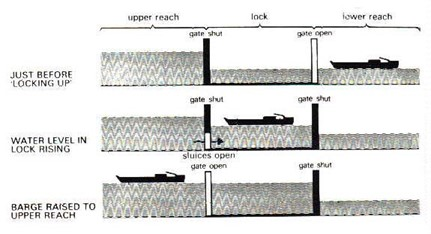
\includegraphics[scale=0.65]{sluismodel.jpg}

\subsubsection{Onderdelen}
Op basis van de schets kunnen we vaststellen dat een sluismodel uit de volgende onderdelen bestaat.

\begin{enumerate}
	\item Een tweetal sluisdeuren. 
	\item Een sluiskolk waarin de schepen in- enuitvaren
	\item een stoplicht om een signaal af te geven voor invaren en uitvaren.
	\item Een nivelleermachine zorgt ervoor dat het water in de sluis op het gewenste niveau wordt gebracht
	\item Een control-system dat ervoor zorgt dat de opdrachten van de sluisbeheerder (geautomatiseerd) worden uitgevoerd
\end{enumerate}
\subsubsection{Werking}

Een schip komt aanvaren en meld zich aan bij de sluismeester. De sluismeester geeft een signaal aan het controlsystem voor het openen van de sluisdeuren, nadat geccontroleerd is of de nivelleermachine al klaar is. Als er ruimte is voor een invarend schip mag het schip dat zoich heeft aangemeld en toestemming heeft  in de sluis varen. Op het moment dat de sluis vol is gaan de sluisdeuren dicht. Eenmaal afgesloten kan de nivelleermachine beginnen om het water in de sluiskolk op het gewenste waterpeil te brengen. Als dit nivelleerprces is afgerond geeft  het controlsystem daan da de sleusdeuren open kunnen.  Als de sleusdeuren open zijn en het uitvaarsignaal is op groen dan moet het schip in de sluis de sluis uitvaren.
\paragraph{extra cases}
Uit het zojuist genoemnde scenario valt het volgende op te maken.
\begin{enumerate}
	\item Een schip geeft een signaal aan een sluismeester.
	\item Er wordt gekeken of er wel plek is in de sluis .
	\item Er wordt gekeken of de nivelleermachine is afgerond.
	\item Er wordt gekeken wat het niveo van de waterpeil in de sluiskolk is.
	\item Er wordt gekeken of de sluisdeuren gereed zijn voor invarende schepen.
\end{enumerate}
\paragraph{Aandachtspunten}
\begin{enumerate}
	\item Voorrang tussen schepen onderling in de sluis?
	\item Hoe lang mag een schip zich in de sluis bevinden?
\end{enumerate} 

%%%%%%%%%%%%%%%%%%%%%%%%%%%%%%%%%%%%%%%%%%%%%%%%%%%%%%%%%%%%%%%%%
\section{Een voorbeeld}

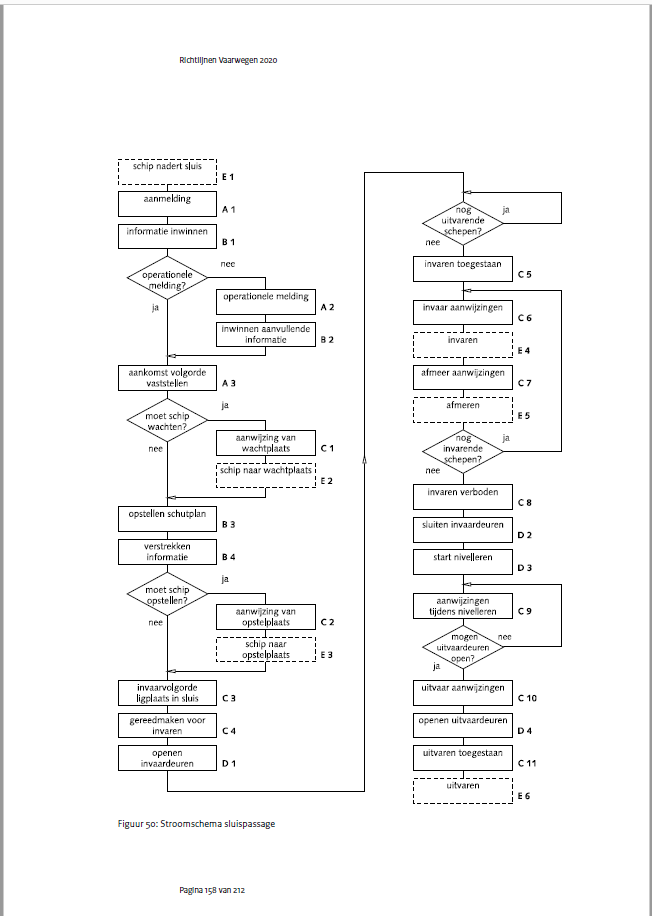
\includegraphics[scale=0.65]{sluispassage.png}

\paragraph{Vooraanmelding}


\paragraph{informatie inwinnen}


\paragraph{operationele melding}


\paragraph{aankomst volgorde}

\paragraph{aanwijzen wachtplaats}


\paragraph{verstrekken informatie}


\paragraph{aanwijzen opstelplaats}

\paragraph{opstellen schutproces}


\paragraph{verstrekken informatie}


\paragraph{invaarvolgorde en ligplaats in sluis}

\paragraph{gereedmaken voor invaren}



\paragraph{openen invaardeuren}




\paragraph{invaren toegestaan}

\paragraph{aanwijzingen voor invaren}
\paragraph{aanwijzingen tijdens afmeren}

\paragraph{invaren verboden}

\paragraph{sluiten invaardeuren}

\paragraph{start nivelleren}

\paragraph{aanzwijzingen voor uitvaren}
\paragraph{openen uitvaardewuren}

\paragraph{uitvaren toegestaan}




\paragraph{brainstorm 22-5-2022}

\subparagraph{invaardeuren en uitvaardeuren}
Gaan we uit van binnendeuren en buitendeuren? Er ontstaat dan een extra ruimte in de sluis. Hoeveel schepen kunnen in deze ruimte? Wat is de maximale wachtreij in deze ruimte en wat zijn de verkeersregels in deze nruimte?
\subparagraph{invaarstoplicht en uitvaarstoplicht}
Als invaren is toegestaan hoe wordt dit dan doorgegeven aan de schepen in de sluis? moeten zij dan uit zichzelf wachten of krijgen zij een signaal dat zij wewl/niet mogen uitvaren? En moeten zij dan kiezen voor links, midden of rechts? Of maakt dat allemaal niets uit?

\subparagraph{invaarwachtrij en uitvaarwachtrij}
Als er meerder schepen in een sluiskolk zitten moet het systeem dan rekeneing houden met het schip dat als eerste is ingevaren en/of het langst in de sluis zit?


%%%%%%%%%%%%%%%%%%%%%%%%%%%%%%%%%%%%%%%%%%%%%%%%%%%%%%%%%%%%%%%%%

\section{Uppaal kripke structuren}


\subsubsection{templates}

\paragraph{Schip}

\paragraph{Sluis}


\paragraph{Aanvoer}


\paragraph{Afvoer}

\paragraph{Pomp}

\paragraph{Pompbediening}


\paragraph{Stoplicht}

\paragraph{Deur}


\subparagraph{case}
Als een schip van rechts binnen komt en sluisdeuren zijn dicht dan moet het stoplicht op rood, de pomnp in transitie van laag naar hoog en niet andersom

\subparagraph{case}
Voor invaren geldt altijd: waterlevel, pomp uit, sluisdeuren open en stoplicht op groen

\subparagraph{case}
uitvarenden hebben voorang op invarenden

\subparagraph{case}
Voor invarenden geldt pomp uit, sleusdeur open en stoplicht op groen
\subparagraph{case}
voor nivelleren geldt pomp is aan, sluisduren zijn doicht en het stoplicht is op rood
\subparagraph{case}
Als een schip vertrekt dan zijn altijd, sleusdeuren open, waterlevel gereed op niveau 5 of 0 en stoplicht direct op groen
\subparagraph{case}
urgent locations; het is niet mogelijk om hier te wachten
\subparagraph{case}
urgent syn; een synchronisatie moet direct worden uitgevoerd als de guards geldig zijn

\subparagraph{case}
als een schip binnen is, en er zijn wachtende schepen, dan moet het stoplicht via oranje naar rood
\subparagraph{case}
committed; als deze staat actief is dan wordt de eerst volgende transitie uitaande van deze state
\subparagraph{case}
als een schjip binnen vaart mnoiet hij ook eft binnen zijn en niet binnenvaren, dit geldt ook voor sluisdeuren en pompen dus deze zijn committed.
\subparagraph{case}

\subparagraph{case}

\subparagraph{case}

\paragraph{Parallele compositie}


\paragraph{Parallele compositie}

\subsubsection{Modeleigenschappel}
\paragraph{Parallele compositie}
Om een sluispark te kunnen modelleren meerdere templates die de verschillende abstracties van het systeem aantonen.

\paragraph{Synchronisatgie}
Zorgt ervoor dat  een transitie die genomen worden in de ene kripke tructuur op hetzelfde moment wordt opgenomen in een andere kripke structuur.



\chapter{CTL logica}


\section{Doel van de test}
\subsection{Wat wordt getest en hoe}


\subsection{toetsen met queries}
\begin{tabular}[t]{rl|rl}%
	\x{lnot}    & \multicolumn{2}{c}{none}\\
	\x{square}  & \x{lozenge}\\
	\x{vee}     & \x{wedge}\\
	\x{vdash}   & \x{models}\\
\end{tabular}




\subsection{Operator: AG}
Voor alle paden


\subsection{Operator: EG}
Uiteindelijk geldt er een pad waarvoor geldt

\subsection{Operator: AF}
Voor alle paden/richtingen vroeg of laat
\subsection{Operator: EF}
Er is een pad
\subsection{Operator: AX}
Alle opvolgende toestanden

~\cite{locke_2020}
\subsection{Operator: EX}
Er bestaat vanaf de volgende minstens 1 state waarvoor geldt
\subsection{Operator: p U q}
Er geldt p tot q
~\cite{gnsguides}
\subsection{Operator: p R q}
q moet waar zijn totdat en inclusief de situatie dat p voor het eerst waar is, als p niet geldig is, dan moet q vooraltjd geldig zijn
\subsection{Fairness}
AG(AF(p))
\begin{verbatim}
	In welke staat de automaat zich ook bevindt, in alle richtingen kom je vroeg of laat een state tegen, waarin p geldig is.
\end{verbatim}
\subsection{Liveness}
\begin{verbatim}
	Altijd en overal geldt: Als p geldt dan geldt vroeg of laat q
	Ookal treedt p nooit p volgens de logica klopt het dan dat q volgt uit p.
	In een situatie, waarin p nooit optreedt, spreekt men van een
	vacuous truth.
\end{verbatim}

\subsubsection{resultaat toetsen met queries}
\begin{center}
	\begin{tabular}{| l | c || r | }
		\hline
		1 &A[] !deadlock  &  TRUE \\ \hline
		2 & A[] not (Sluis.Tussenstop5 \&\& Deur.Klaar\_voor\_uitvaart)  &  Disconnected \\ \hline
		3 & A[]  (Sluis.Voorbereiden imply Deur.Dicht)   &  TRUE\\   \hline
		4 &A[]  (Deur.Dicht imply Counter==0)   & TRUE  \\   \hline
		5 & A[]  (Buitenstoplicht.Groen imply invaren\_allowed==true)  &  TRUE \\ \hline
		6 & A[] ! (Binnenstoplicht.Groen imply invaren\_allowed==false)  & FALSE \\ \hline
		7 & A[]  (globale\_tijd>30)   &  FALSE\\    \hline
		8 & E<>  (Schip.Stoppen and (Counter >5))   & Ship not a structure  \\   \hline
		9 & A[] (Schip.Vertrekken imply Sluisdeur.Dicht)  &  -  \\   \hline
		\hline
	\end{tabular}
\end{center}

\subsubsection{Script voor uppaal template}
\begin{verbatim}
	
	Queries
	Sluis.Draining-->Deuren.laag_open
	Deuren.laag_open-->Stoplicht.Green
	E<> (Ship.ship_can_move&&Stoplicht.Green)
	A[] not (Stoplicht.Green && not (Deuren.hoog_open||Deuren.laag_open||Deuren.stopgaplow1||Deuren.stopgaplow2||Deuren.stopgaphigh1||Deuren.stopgaphigh2))
	A[] not ((Deuren.hoog_open||Deuren.laag_open||Deuren.Opening_laag||Deuren.Opening_hoog||Deuren.Closing_hoog||Deuren.Closing_laag) && (Sluis.Draining||Sluis.Filling||Sluis.draining2||Sluis.Filling2))
	Sensor.Wait-->Sensor.Wait
	Stoplicht.Green-->Stoplicht.Green
	(Deuren.hoog_open||Deuren.laag_open)-->(Deuren.laag_open||Deuren.hoog_open)
	Deuren.laag_open-->Deuren.Closed
	Deuren.hoog_open-->Deuren.Closed
	Deuren.Closed-->Stoplicht.Red
	Ship.ship_can_move-->Deuren.Closed
	Deuren.hoog_open-->Stoplicht.Green
	Ship.ship_can_move-->Stoplicht.Green
	A[] not (Deuren.laag_open && Deuren.hoog_open)
	Ship.ship_can_move-->Ship.ship_can_move
	A[] not (Deuren.laag_open && Sluis.water != Sluis.water_laag)
	A[] not (Deuren.hoog_open && Sluis.water != Sluis.water_hoog)
	A[]not deadlock
	
	Project declaraties
	//Declarations
	
	chan boot_hoog;
	chan boot_laag;
	chan changedoor_low;
	chan changedoor_high;
	chan ship_moves;
	chan ship_abletomove;
	chan changelight;
	
	\\Sluis declaraties
	const int water_laag=0;
	const int water_hoog=10;
	const int water_median=(water_hoog+water_laag)/2;
	int[water_laag,water_hoog] water=water_median;
	clock x;
	\\Stoplicht declaraties
	
	\\Ship declaraties
	clock x;
	\\Sensor declaraties
	
	\\Deuren declaraties
	bool stoplicht_hoog=false;
	bool stoplicht_laag=false;
	clock x;
	
	
	\\System declaraties
	system Deuren,Sensor,Sluis,Ship,Stoplicht;
	
	
	Uitleg
	Als het schip boven is, dan is waterlvel gelijk aan hoog, filling valve is dicht, lower gates zijn gesloten, uppergates zijn open,empty valve is dicht. 
	Schip is in waterlock, waterlevel is hoog, filling valve is dicht, lower gates gesloten, upper gates gesloten, empty valve is open. 
	Schip is dan laag, waterlevel gelijk aan laag, filling valve is dicht, lowergates zijn open, uppergates zijn dicht, empty valve is dicht.
	AtArrivalHigh
	
	AtArrivalLow
	Als schip beneden is dan is waterlevel gelijk aan laag, filling valve is dicht, lower gates zijn open, upper gates zijn dicht, empty valve is open. 
	Schip is in water lock, waterlevel is laag, flilling valve is open, lower gates zijn gesloten, upper gates zij gesloten, empty valve is dicht,. 
	Schip is dan hoog, waterlevel is gelijk aan hoog, filling valve is dicht, uppergates zijn open, lowergates zijn dicht, filling valve is dicht
	
	
	
\end{verbatim}
\begin{gather*}
	D=\Set{x\in\nat}{1\le x\le 100}\\
	D=\Set[\big]{x\in\nat}{1\le x\le 100}\\
	D=\Set[\Big]{x\in\nat}{1\le x\le 100}\\
	D=\Set[\bigg]{x\in\nat}{1\le x\le 100}\\
	D=\Set[\Bigg]{x\in\nat}{1\le x\le 100}\\
	D=\Set*{x\in\nat}{1\le x\le \frac{200}{2}}
\end{gather*}

\begin{align}
	\alpha &= \beta + \gamma * \lambda \\
	\alpha &= \beta + \gamma * \lambda \\
	\alpha &= \beta + \gamma * \lambda \\
	\theta &= \frac{\alpha}{4}
\end{align} 

%  https://www.stat.cmu.edu/~brian/latex/symbols/symbols.html
% https://tex.loria.fr/ctan-doc/macros/latex/doc/html/fntguide/node18.html
% https://observablehq.com/@s-haensch/latex-notation
% http://tdc-www.harvard.edu/tdcprop1/help/symbols/
% http://new.math.uiuc.edu/oldnew/netgeom/advice/to-texpad.html
% https://www.overleaf.com/learn/latex/List_of_Greek_letters_and_math_symbols
% https://jblevins.org/log/greek
% https://latex-tutorial.com/symbols/greek-alphabet/
% https://latex-programming.fandom.com/wiki/List_of_LaTeX_symbols
% https://physicsanduniverse.com/latex-symbols-and-using-them-to-write-equations/
% http://tug.ctan.org/info/symbols/comprehensive/symbols-a4.pdf
% https://tex.stackexchange.com/questions/99772/how-to-insert-greek-letters-having-trouble-with-greekletter
% https://texblog.org/2012/03/15/greek-letters-in-text-without-changing-to-math-mode/
% https://www.avantixlearning.ca/microsoft-word/how-to-insert-greek-letters-or-symbols-in-microsoft-word/
%
%
%




$S is a set of finite states$\\
$S0 \subseteq S is de set van initiele statess$ \\
$S0 \subseteq S xS  is een transitie relatie die totaal moet zij, dat betekent, dat voor elke state s \in S er een stats is s' \in S zodat R(s,s')$
$L\stock a$

$\forall x\,\exists y \implies $

$\mtproforall x\,\mtproexists y \cap \subset \in \vee \diamondsuit \dashv \ni \pm$


\subsubsection{onderdeleel van de test}
\paragraph{resultaat}
\subparagraph{verklareing}


\subsection{liveness}


\subsection{safety}


\subsection{zeno vrij}
Geen enkele state kan oneindig een transitie uitvoeren. Elke state heeft een uitgaande transitie.

\subsection{deadlocks}


 
\section{testresultaten}
Om een goed verhaal op te stellen, moet vooraf aan enkele voorwaarden
worden voldaan. De eerste voorwaarde is de geschiktheid van het
afstudeerproject. Als een afstudeerproject niet tot keuzes leidt, kan
men zich afvragen of dat wel een echte afstudeeropdracht is. Een
afstudeerproject zonder onderzoeksaspecten is ook verdacht. Daarnaast
moet een afstudeerproject passen in het profiel van een opleiding om
beoordeelbaar te zijn. De andere voorwaarde voor goed een verhaal is
de registratie van werkzaamheden tijdens het a


\begin{tabular}{|l|l {2cm} |l|l|l|l|l|l|l|l|} \hline
	\multicolumn{10}{|l|}{REQ traceabilitymatrix}                                                               \\ \hline
	\multicolumn{4}{|l|}{project name}   &\multicolumn{6}{|l|}{Created designed by}                           \\ \hline
	\multicolumn{4}{|l|}{release no}   &\multicolumn{6}{|l|}{Created on}                           \\ \hline
	\multicolumn{4}{|l|}{version}   &\multicolumn{6}{|l|}{Reviewed on}                           \\ \hline
	\multicolumn{4}{|l|}{Test title}   &\multicolumn{6}{|l|}{Reviewed by}                           \\ \hline
	\multicolumn{4}{|l|}{Description}   &\multicolumn{6}{|l|}{ }                           \\ \hline 		
	\multicolumn{10}{|l|}{ }   																\\ \hline
	\multicolumn{10}{|l|}{Pre condition}                                                               \\ \hline
	\multicolumn{10}{|l|}{Dependencies}                                                               \\ \hline
	\multicolumn{10}{|l|}{ }   															\\ \hline
	\multicolumn{2}{|l|}{REQID} & descr & ST &Designdoc &codemod.&t.caseID &T.caseNme & manu& testedon \\ \hline
	 
\end{tabular}






\subsection{Testcases}		

Om een goed verhaal op te stellen, moet vooraf aan enkele voorwaarden
worden voldaan. De eerste voorwaarde is de geschiktheid van het
afstudeerproject. Als een afstudeerproject niet tot keuzes leidt, kan
men zich afvragen of dat wel een echte afstudeeropdracht is. Een
afstudeerproject zonder onderzoeksaspecten is ook verdacht. Daarnaast
moet een afstudeerproject passen in het profiel van een opleiding om
beoordeelbaar te zijn. De andere voorwaarde voor goed een verhaal is
de registratie van werkzaamheden tijdens het a



\begin{tabular}{|l|l|l|l|l|l|l|} \hline
	\multicolumn{7}{|l|}{project name}                                                               \\ \hline
	\multicolumn{4}{|l|}{Test case ID}   &\multicolumn{3}{|l|}{Test designed by}                           \\ \hline
	\multicolumn{4}{|l|}{test priority (low/medium/high)}   &\multicolumn{3}{|l|}{Test design date}                           \\ \hline
	\multicolumn{4}{|l|}{Module name}   &\multicolumn{3}{|l|}{Test executed by}                           \\ \hline
	\multicolumn{4}{|l|}{Test title}   &\multicolumn{3}{|l|}{Test execution date}                           \\ \hline
	\multicolumn{4}{|l|}{Description}   &\multicolumn{3}{|l|}{ }                           \\ \hline 		
	\multicolumn{7}{|l|}{ }   																\\ \hline
	\multicolumn{7}{|l|}{Pre condition}                                                               \\ \hline
	\multicolumn{7}{|l|}{Dependencies}                                                               \\ \hline
	\multicolumn{7}{|l|}{ }   															\\ \hline
	Step  &  Test steps & Test data & expected result &Acual result &Streee (pass or fail)&notes  \\ \hline
	
\end{tabular}

\subsubsection{Een schip komt aanvaren}	

\subsubsection{Een schip moet wachten}

\subsubsection{Een schip komt van boven naar beneden}

\subsubsection{De sluis is vol: hoe lang mkoet een schip wachten}


\subsubsection{Een schip wil in de sluis koers wijzigen}

\subsubsection{De volgorde in  de wachtrij}


\subsubsection{Aantal schepen in de wachtrij}	

\subsubsection{Maximale doorlooptijd }

\subsubsection{Minimale doorlooptijd 
	
	
	
	Black box testing: product test  zonder kennis van code, implementatie of interne paden
	Alpha testimg: bugs en issues testen voor de release; soort van acceptatietest
	Functioneel testen: require,emnnt testen op input/output en requirement omschrijving webinterface
	Domain testing: applicaties testen met normale input; waarvan het doel is om te testen of de app waardenbereik hanteert
	Gebruikeraaceptatieteast:
	Interface testing: om de communicatie tussen 2 interfaces te testen
	Vulnerability testing: testen op kwetsbaarheden webinterface
	Configuration testing: de app testen met meerdere hardware en software combinaties; verschillende browsers, OS; IoT cloud
	Applicatie test: script om de gehele applicatie te testen
	Negative testing: test de ap[p op negatieve waarden waaronder 
	Interoperabiliteit : test of het systeem kan communiceren met andere systemen; zoals cloud/wifi/netwerk
	Complianc testing: test of het systeem voldoiet aan de stabndaarden
	Loop testing: test over de loops in de app
	Component testing: elk systee,mcomponent wordt getest
	Dynamic testing: test de code in natuurlijke omgeving
	Parralel testing: systeem testen tegelijk op meerdere platformen
	Operational acceptance testing:
	Module testing: test de procedures, classes, subroutine of subprogramma’s
	Workflow testing: wordt de serie taken juist uitgevoerd
	Storage testing: wordt de relevantedata opgeslagen
	Recovery testing: wordt de systeem ook getest op hoe het reageert op cradshes
	Concurrency testing: hoe reageert de app als er moderne gebruikers tegelijkj toegevoegd zijn
	Thread testing: key functionaliteit van een thread testen
	Desctructive test: apparaat wordt geteast op het  omgaan met verkeerde informatie
	Test-driven-development: test ontwikkelen voor elke functionalitei
	Data driven testing:
	Monkey testing: de app testen zonder  vooraf gedefinieerd
	Embedded testing:
	Rest api testing:
	Gui testing:
	Automated vs manual testing:>
	Unit test: individuele componenten testen
	Integrale test: werkt de software als onderdeel van een groot systeem
	System test: test de werking van het volledige product
	Sanity Test: is het product rationeel ontwikkeld
	Smokey test: werken de kritische functionaliteiten
	Regressie test: test of een wijziging in de code geen invloed heeft op meer processen of taken
	non-functionele testebn
	Boundary testen: testen op partities
	Decision table testing: wat te  doen als er een incoerveld verkeerd is ingevuld
	Stat transition testing: toont het systeem de informatie bij een weijziging
	Agile teting
	Continuous testoing
	Performance test: hoeveel data
	Load testing: is laadtijd van het systeem relevant
	Stress test: test van het systeem onder zware condities
	Volumte testin: een volume aan data testen
	Scalability testing systeem testen bij extreem data verkeer
	Performance testing
	Response time testing: hoe lang durut het voordat het systeem reageert
	Benchmark testing: vergelijken van kwaliteitsattribh8uten
	Endurance testing: systeem testen over lange periode
	Reliabilityb testing: kan het systeem foutloos draaien over een lange periode
	Test metrics
	End-to-e nd testing: test hele systeem van end bnaa alle
	Externe interfaces: test op afhankelijkheden; data integriteit; communicatie met andere systemen, interfaces en databases
	Exploratory testing: testing on the fly
	Mutation testing: een controle op kleine wijzigingen van bijv namen van variabelen of functies
	Ad-hoc testing: willekeurig overal testen waar vermoedelijk fouten zitten in het key-drives-framework
	risk -based-testing: in kaart brengen van
	Backend testing: bijv dedatabase-tabel van telemetrie
	Localization testing: regio gericht testen
	Ontogonaal testen: testen van testcases
	Pilot testing: feasibility; time;cost;risk;performance
	Model base testen: testen volgens een model
	Grey box testing
	Whitelabeel testing: test hoe ebruiksvriendelijk het product is
	
	
	\subsection{Reparaties}
	
	\subsection{Resulaat annalyse}
	
	
	%%%%%%%%%%%%%%%%%%%%%%%%%%%%%%%%%%%%%%%%%%%%%%%%%%%%%%%%%%%%%%
	\subsubsection{Editor}
	
	
	%%%%%%%%%%%%%%%%%%%%%%%%%%%%%%%%%%%%%%%%%%%%%%%%%%%%%%%%%%%%%%
	
	\subsubsection{Concrete simulator}
	
	
	%%%%%%%%%%%%%%%%%%%%%%%%%%%%%%%%%%%%%%%%%%%%%%%%%%%%%%%%%%%%%%
	
	\subsubsection{verifier}
	%%%%%%%%%%%%%%%%%%%%%%%%%%%%%%%%%%%%%%%%%%%%%%%%%%%%%%%%%%%%%%
	
	\subsubsection{Yggdrasil} 

 




	\chapter{Testresultaten}
	
	\section{Inleiding}
	In het hoofdverslag moet een rode draad aanwezig zijn,
	zodanig dat het een leesbaar artikel wordt. Deze leesbaarheid houdt in
	dat het publiceerbaar moet zijn in een vakblad. Dit betekent dat voor
	de onderbouwing noodzakelijke gegevens (tabellen, grafieken en
	tekeningen) die de leesbaarheid kunnen verlagen, worden opgenomen in
	bijlagen. Bijlagen worden niet gepubliceerd.
	
	
	\section{verwachte testresultaten}
	
	Om een goed verhaal op te stellen, moet vooraf aan enkele voorwaarden
	worden voldaan. De eerste voorwaarde is de geschiktheid van het
	afstudeerproject. Als een afstudeerproject niet tot keuzes leidt, kan
	men zich afvragen of dat wel een echte afstudeeropdracht is. Een
	afstudeerproject zonder onderzoeksaspecten is ook verdacht. Daarnaast
	moet een afstudeerproject passen in het profiel van een opleiding om
	beoordeelbaar te zijn. De andere voorwaarde voor goed een verhaal is
	de registratie van werkzaamheden tijdens het afstudeerproject. Dit
	voorkomt dat men dingen vergeet.
	
	\section{Testopstelling}
	
	Om een goed verhaal op te stellen, moet vooraf aan enkele voorwaarden
	worden voldaan. De eerste voorwaarde is de geschiktheid van het
	afstudeerproject. Als een afstudeerproject niet tot keuzes leidt, kan
	men zich afvragen of dat wel een echte afstudeeropdracht is. Een
	afstudeerproject zonder onderzoeksaspecten is ook verdacht. Daarnaast
	moet een afstudeerproject passen in het profiel van een opleiding om
	beoordeelbaar te zijn. De andere voorwaarde voor goed een verhaal is
	de registratie van werkzaamheden tijdens het afstudeerproject. Dit
	voorkomt dat men dingen vergeet.
	
	
	\begin{center}
		\figuur{width=\columnwidth}{plaatjes/putty\_config.png}{PNGR}{Variabele breedte (png)}
	\end{center}
	
 
	
	
	% Insert the following commented line before \begin{document}:
		% \usepackage{multirow} 
		
		\begin{tabular}{|l|l|l|l|l|l|l|} \hline
			\multicolumn{7}{|l|}{project name}                                                               \\ \hline
			\multicolumn{4}{|l|}{Test case ID}   &\multicolumn{3}{|l|}{Test designed by}                           \\ \hline
			\multicolumn{4}{|l|}{test priority (low/medium/high)}   &\multicolumn{3}{|l|}{Test design date}                           \\ \hline
			\multicolumn{4}{|l|}{Module name}   &\multicolumn{3}{|l|}{Test executed by}                           \\ \hline
			\multicolumn{4}{|l|}{Test title}   &\multicolumn{3}{|l|}{Test execution date}                           \\ \hline
			\multicolumn{4}{|l|}{Description}   &\multicolumn{3}{|l|}{ }                           \\ \hline 		
			\multicolumn{7}{|l|}{ }   																\\ \hline
			\multicolumn{7}{|l|}{Pre condition}                                                               \\ \hline
			\multicolumn{7}{|l|}{Dependencies}                                                               \\ \hline
			\multicolumn{7}{|l|}{ }   															\\ \hline
			Step  &  Test steps & Test data & expected result &Acual result &Streee (pass or fail)&notes  \\ \hline
			\multicolumn{7}{|l|}{Post condition}                                                               \\ \hline
		\end{tabular}
		
		Laat je verslag lezen door een niet bij het afstudeerproject betrokken
		persoon. Meestal ziet die al snel waarin je verslag tekort schiet.
		 
		
		
		\section{Webserver}
		
		\begin{usecase}
			\addheading{Actor}{System user} 
			\addrow{Precondition}{The system, shows, in the form part of an object type, the number   indication.}
			\addrow{Postcondition}{A disconnected number indicating the type of `other constructed object'.}
			\addmulrow{Main path (M)}{\item User selects \ldots
				\item System demands \ldots}
		\end{usecase}
	 
		
		
		
		 
		
		
		\section{MQTT subscribing}
		
		\begin{usecase}
			\addheading{Testcase}{Result} 
			\addrow{est case ID}{The system, shows, in the form part of an object type, the number   indication.}
			\addrow{Test priority (Low/Medium/High)}{A disconnected number indicating the type of `other constructed object'.}
			\addrow{Module Name:}{A disconnected number indicating the type of `other constructed object'.}
			\addrow{Test Designed By Name of the Tester.}{A disconnected number indicating the type of `other constructed object'.}
			\addrow{ Test Designed Date:}{ }
			\addrow{Test Executed By }{ }
			\addrow{ Test Execution Date: }{ }
			\addrow{ Test Title/Name:}{ }
			\addrow{ Test Summary/Description:}{ }
			\addrow{ Pre-conditions:}{ }
			\addrow{ Dependencies:}{ }
			\addrow{ Test Steps:}{ }
			\addrow{ Pro Tip: }{ }
			\addrow{ Test Data:}{ }
			\addrow{ Expected Result:}{ }
			\addrow{ Post-condition:}{ }
			\addrow{ Actual result:}{ }
			\addrow{ Status (Pass/Fail):}{ }
			\addrow{ Notes/Comments/Questions:}{ }
			\addrow{ Optional}{ }
			\addrow{ Defect ID/Link:}{ }
			\addrow{ Test Type/Keywords:}{ }
			\addrow{Requirements: }{ }
			\addrow{ Attachments/References:}{ }
			\addrow{ Automation? (Yes/No):}{ }
			
		\end{usecase}
		
		%https://www.softwaretestinghelp.com/test-case-template-examples/
		%\include{reparaties}   
	
		\chapter{reparaties}
		
		\section{Inleiding}
		Om een goed verhaal op te stellen, moet vooraf aan enkele voorwaarden
		worden voldaan. De eerste voorwaarde is de geschiktheid van het
		afstudeerproject. Als een afstudeerproject niet tot keuzes leidt, kan
		men zich afvragen of dat wel een echte afstudeeropdracht is. Een
		afstudeerproject zonder onderzoeksaspecten is ook verdacht. Daarnaast
		moet een afstudeerproject passen in het profiel van een opleiding om
		beoordeelbaar te zijn. De andere voorwaarde voor goed een verhaal is
		de registratie van werkzaamheden tijdens het afstudeerproject. Dit
		voorkomt dat men dingen vergeet.
		
		\section{Watchdog timer}
		Om een goed verhaal op te stellen, moet vooraf aan enkele voorwaarden
		worden voldaan. De eerste voorwaarde is de geschiktheid van het
		afstudeerproject. Als een afstudeerproject niet tot keuzes leidt, kan
		men zich afvragen of dat wel een echte afstudeeropdracht is. Een
		afstudeerproject zonder onderzoeksaspecten is ook verdacht. Daarnaast
		moet een afstudeerproject passen in het profiel van een opleiding om
		beoordeelbaar te zijn. De andere voorwaarde voor goed een verhaal is
		de registratie van werkzaamheden tijdens het afstudeerproject. Dit
		voorkomt dat men dingen vergeet.
		
		\section{OS-taak wifi-reconnect }
		Om een goed verhaal op te stellen, moet vooraf aan enkele voorwaarden
		worden voldaan. De eerste voorwaarde is de geschiktheid van het
		afstudeerproject. Als een afstudeerproject niet tot keuzes leidt, kan
		men zich afvragen of dat wel een echte afstudeeropdracht is. Een
		afstudeerproject zonder onderzoeksaspecten is ook verdacht. Daarnaast
		moet een afstudeerproject passen in het profiel van een opleiding om
		beoordeelbaar te zijn. De andere voorwaarde voor goed een verhaal is
		de registratie van werkzaamheden tijdens het afstudeerproject. Dit
		voorkomt dat men dingen vergeet.
		%\include{toetsing}
		\chapter{Projectreflectie}
		
	 
		\section{Het ontwikkelproces}
		Om een goed verhaal op te stellen, moet vooraf aan enkele voorwaarden
		worden voldaan. De eerste voorwaarde is de geschiktheid van het
		afstudeerproject. Als een afstudeerproject niet tot keuzes leidt, kan
		men zich afvragen of dat wel een echte afstudeeropdracht is. Een
		afstudeerproject zonder onderzoeksaspecten is ook verdacht. Daarnaast
		moet een afstudeerproject passen in het profiel van een opleiding om
		beoordeelbaar te zijn. De andere voorwaarde voor goed een verhaal is
		de registratie van werkzaamheden tijdens het afstudeerproject. Dit
		voorkomt dat men dingen vergeet.
		
		
		Laat je verslag lezen door een niet bij het afstudeerproject betrokken
		persoon. Meestal ziet die al snel waarin je verslag tekort schiet.
		\section{Hoe is getest}
		Om een goed verhaal op te stellen, moet vooraf aan enkele voorwaarden
		worden voldaan. De eerste voorwaarde is de geschiktheid van het
		afstudeerproject. Als een afstudeerproject niet tot keuzes leidt, kan
		men zich afvragen of dat wel een echte afstudeeropdracht is. Een
		afstudeerproject zonder onderzoeksaspecten is ook verdacht. Daarnaast
		moet een afstudeerproject passen in het profiel van een opleiding om
		beoordeelbaar te zijn. De andere voorwaarde voor goed een verhaal is
		de registratie van werkzaamheden tijdens het afstudeerproject. Dit
		voorkomt dat men dingen vergeet.
		
		
		Laat je verslag lezen door een niet bij het afstudeerproject betrokken
		persoon. Meestal ziet die al snel waarin je verslag tekort schiet.
		\section{Welke coding standaarden}
		Om een goed verhaal op te stellen, moet vooraf aan enkele voorwaarden
		worden voldaan. De eerste voorwaarde is de geschiktheid van het
		afstudeerproject. Als een afstudeerproject niet tot keuzes leidt, kan
		men zich afvragen of dat wel een echte afstudeeropdracht is. Een
		afstudeerproject zonder onderzoeksaspecten is ook verdacht. Daarnaast
		moet een afstudeerproject passen in het profiel van een opleiding om
		beoordeelbaar te zijn. De andere voorwaarde voor goed een verhaal is
		de registratie van werkzaamheden tijdens het afstudeerproject. Dit
		voorkomt dat men dingen vergeet.
		
		
		Laat je verslag lezen door een niet bij het afstudeerproject betrokken
		persoon. Meestal ziet die al snel waarin je verslag tekort schiet.
		\section{Hoe zijn bugs opgelost en gedocumenteerd}
		Om een goed verhaal op te stellen, moet vooraf aan enkele voorwaarden
		worden voldaan. De eerste voorwaarde is de geschiktheid van het
		afstudeerproject. Als een afstudeerproject niet tot keuzes leidt, kan
		men zich afvragen of dat wel een echte afstudeeropdracht is. Een
		afstudeerproject zonder onderzoeksaspecten is ook verdacht. Daarnaast
		moet een afstudeerproject passen in het profiel van een opleiding om
		beoordeelbaar te zijn. De andere voorwaarde voor goed een verhaal is
		de registratie van werkzaamheden tijdens het afstudeerproject. Dit
		voorkomt dat men dingen vergeet.
		
		
		Laat je verslag lezen door een niet bij het afstudeerproject betrokken
		persoon. Meestal ziet die al snel waarin je verslag tekort schiet.
		\section{Hoe verliep het deployment proces}
		%\section{Welke hardware/software requirements voor de otnwikkelomgeving van de prototype}
		\section{Welke repo is gebruikt en waarom}
		Om een goed verhaal op te stellen, moet vooraf aan enkele voorwaarden
		worden voldaan. De eerste voorwaarde is de geschiktheid van het
		afstudeerproject. Als een afstudeerproject niet tot keuzes leidt, kan
		men zich afvragen of dat wel een echte afstudeeropdracht is. Een
		afstudeerproject zonder onderzoeksaspecten is ook verdacht. Daarnaast
		moet een afstudeerproject passen in het profiel van een opleiding om
		beoordeelbaar te zijn. De andere voorwaarde voor goed een verhaal is
		de registratie van werkzaamheden tijdens het afstudeerproject. Dit
		voorkomt dat men dingen vergeet.
		\section{Ontwikkelomgeving}
		Om een goed verhaal op te stellen, moet vooraf aan enkele voorwaarden
		worden voldaan. De eerste voorwaarde is de geschiktheid van het
		afstudeerproject. Als een afstudeerproject niet tot keuzes leidt, kan
		men zich afvragen of dat wel een echte afstudeeropdracht is. Een
		afstudeerproject zonder onderzoeksaspecten is ook verdacht. Daarnaast
		moet een afstudeerproject passen in het profiel van een opleiding om
		beoordeelbaar te zijn. De andere voorwaarde voor goed een verhaal is
		de registratie van werkzaamheden tijdens het afstudeerproject. Dit
		voorkomt dat men dingen vergeet.
		
		
		Laat je verslag lezen door een niet bij het afstudeerproject betrokken
		persoon. Meestal ziet die al snel waarin je verslag tekort schiet.
		\section{testproces}
		Om een goed verhaal op te stellen, moet vooraf aan enkele voorwaarden
		worden voldaan. De eerste voorwaarde is de geschiktheid van het
		afstudeerproject. Als een afstudeerproject niet tot keuzes leidt, kan
		men zich afvragen of dat wel een echte afstudeeropdracht is. Een
		afstudeerproject zonder onderzoeksaspecten is ook verdacht. Daarnaast
		moet een afstudeerproject passen in het profiel van een opleiding om
		beoordeelbaar te zijn. De andere voorwaarde voor goed een verhaal is
		de registratie van werkzaamheden tijdens het afstudeerproject. Dit
		voorkomt dat men dingen vergeet.
		\section{Build proces}
		Om een goed verhaal op te stellen, moet vooraf aan enkele voorwaarden
		worden voldaan. De eerste voorwaarde is de geschiktheid van het
		afstudeerproject. Als een afstudeerproject niet tot keuzes leidt, kan
		men zich afvragen of dat wel een echte afstudeeropdracht is. Een
		afstudeerproject zonder onderzoeksaspecten is ook verdacht. Daarnaast
		moet een afstudeerproject passen in het profiel van een opleiding om
		beoordeelbaar te zijn. De andere voorwaarde voor goed een verhaal is
		de registratie van werkzaamheden tijdens het afstudeerproject. Dit
		voorkomt dat men dingen vergeet.
		\section{Deployment proces}
		Om een goed verhaal op te stellen, moet vooraf aan enkele voorwaarden
		worden voldaan. De eerste voorwaarde is de geschiktheid van het
		afstudeerproject. Als een afstudeerproject niet tot keuzes leidt, kan
		men zich afvragen of dat wel een echte afstudeeropdracht is. Een
		afstudeerproject zonder onderzoeksaspecten is ook verdacht. Daarnaast
		moet een afstudeerproject passen in het profiel van een opleiding om
		beoordeelbaar te zijn. De andere voorwaarde voor goed een verhaal is
		de registratie van werkzaamheden tijdens het afstudeerproject. Dit
		voorkomt dat men dingen vergeet.
		\section{Support en issue management}
		Om een goed verhaal op te stellen, moet vooraf aan enkele voorwaarden
		worden voldaan. De eerste voorwaarde is de geschiktheid van het
		afstudeerproject. Als een afstudeerproject niet tot keuzes leidt, kan
		men zich afvragen of dat wel een echte afstudeeropdracht is. Een
		afstudeerproject zonder onderzoeksaspecten is ook verdacht. Daarnaast
		moet een afstudeerproject passen in het profiel van een opleiding om
		beoordeelbaar te zijn. De andere voorwaarde voor goed een verhaal is
		de registratie van werkzaamheden tijdens het afstudeerproject. Dit
		voorkomt dat men dingen vergeet.
		\section{Source control}
		Om een goed verhaal op te stellen, moet vooraf aan enkele voorwaarden
		worden voldaan. De eerste voorwaarde is de geschiktheid van het
		afstudeerproject. Als een afstudeerproject niet tot keuzes leidt, kan
		men zich afvragen of dat wel een echte afstudeeropdracht is. Een
		afstudeerproject zonder onderzoeksaspecten is ook verdacht. Daarnaast
		moet een afstudeerproject passen in het profiel van een opleiding om
		beoordeelbaar te zijn. De andere voorwaarde voor goed een verhaal is
		de registratie van werkzaamheden tijdens het afstudeerproject. Dit
		voorkomt dat men dingen vergeet.
		\subsubsection{subsubsection}
		
		Om een goed verhaal op te stellen, moet vooraf aan enkele voorwaarden
		worden voldaan. De eerste voorwaarde is de geschiktheid van het
		afstudeerproject. Als een afstudeerproject niet tot keuzes leidt, kan
		men zich afvragen of dat wel een echte afstudeeropdracht is. Een
		afstudeerproject zonder onderzoeksaspecten is ook verdacht. Daarnaast
		moet een afstudeerproject passen in het profiel van een opleiding om
		beoordeelbaar te zijn. De andere voorwaarde voor goed een verhaal is
		de registratie van werkzaamheden tijdens het afstudeerproject. Dit
		voorkomt dat men dingen vergeet.
		\section{Rollback procedures}
		\subsubsection{subsubsection}
		
		Om een goed verhaal op te stellen, moet vooraf aan enkele voorwaarden
		worden voldaan. De eerste voorwaarde is de geschiktheid van het
		afstudeerproject. Als een afstudeerproject niet tot keuzes leidt, kan
		men zich afvragen of dat wel een echte afstudeeropdracht is. Een
		afstudeerproject zonder onderzoeksaspecten is ook verdacht. Daarnaast
		moet een afstudeerproject passen in het profiel van een opleiding om
		beoordeelbaar te zijn. De andere voorwaarde voor goed een verhaal is
		de registratie van werkzaamheden tijdens het afstudeerproject. Dit
		voorkomt dat men dingen vergeet.
		
		
		
		\begin{center}
			\figuur{scale=0.45,angle=270}{plaatjes/agp.pdf}{PDFA}{Vaste breedte
				(pdf)}
		\end{center}
	
	
	\chapter{Conclusie}
		
		%\hoofdstuk{Persoonlijk verslag}

In de evaluatie reflecteer je over je eigen afstudeerproces. Daarbij
moet je vooral letten op de leereffecten. Welke competenties had je
nodig? Welke competenties kwam je tekort en moest je zelf verwerven?
Waren dit algemene of specifieke competenties?  Voldeden de
beroepscompetenties aan de standaard van het \emph{HBO-I} (analyseren,
adviseren, ontwerpen, realiseren en beheren)?  Vielen de algemene
competenties in de vijf categorieën van de \emph{Dublin
Descriptoren}\footnote{Dublin Descriptoren zijn eisen aan de
competenties voor de bachelor en master studies aan universiteiten en
hogescholen in Europa.} zoals het verkrijgen van kennis en inzicht,
het toepassen van kennis en inzicht, het maken van onderbouwde keuzen
(oordeelsvorming), het communiceren (schriftelijk en mondeling) en het
verkrijgen van leervaardigheden?

   %(optioneel) uitvoering
		%\hoofdstuk{Evaluatie}
		\chapter{Evaluatie}
		
		\section{Defintie}
		
		Wat is het probleem precies bij het bedrijf en is de opdracht complex genoeg. Bij het presenteren van het mandaat leken de definitie, onderzoek, ontewrrp en ontwikkelfase al te kunnen starten vanaf week 8. Dit werd verschoven naar week 12
		
		Welke hardware/software requirements voor de otnwikkelomgeving van de prototype
		Developer machine software requirements (i.e. required development environment)
		
		\section{Onderzoek}
		Onderzoek nar IoT heeft algemene resutlaten opgeleverd
		Onderzoek naar MQTT heeft aleemn maar relebvante informatie opgeleverd over het security aspect van mqtt en de verschillende  versies van mqtt
		Onderzoek naar alternatieven MQTT
		Onderzoek naar IoT platformen
		Onderzoek naar ontwikkelmogelijkheden IoT cloud platformn
		Onderzoek naar bruikbaarheid IoT platformen
		Onderzoek naar prijsmodellen platformen
		Onderzoek webnserver onboarding interface specificatgies
		Onderzoek naar ESp32
		Onderzoek naar freeRTOS
		Onderzoek naar Espressif voor esp8266
		Onderzoek naar esp32 nodemcu
		Onderzoek naar Provisioning
		Onderzoek naar dashboard provisioning
		Revieww van de onderzoeksresultaten
		
		
		\section{Analyse}
		
		Het meest complexe onderdeel is de platform selectie. De verschillen tussen de IoT cloud platforms zijn minimaal en de hoeveelheid platforms lijkt alleen maar toe te nemen. Door grenzen te trekken in de hoeveelheid data en achtergrondinformatie online is het mogelijk om een deel van dit kant van IT te begrijpen en erop in te spelen.
		Proof of concept
		Revieww van de analyse resultaten
		
		
		\section{Ontwerp}
		
		Klassendiagram
		Filenaming in het diagram
		Modulename en klassennamen
		Revieww van de ontwerpresultaten
		
		
		\section{Ontwikkel}
		Het meest interessant en uitdagende onderdeel is het ontwikkelen van de firmware geweest. De ESPRESSIF SDK biedt ontwikkelaars de mogelijkheden en documentatie om een product te ontwikkelen dat op van toepassing kan zijn op veel projecten. Ik zou elke programmeer die meer kennis en ervaring wil opdoen met real-time development tijd en aandacht te besteden aan dit IT-aspect.
		
		Wat is er nodig voor MQTT en thingsboard
		Watchdog timers
		Welke coding standaarden
		Coding standards including file naming conventions and language specific standards.
		Het ontwikkelproces
		The development process, how work is tracked, assigned and updated and what tools are used.
		Hoe zijn bugs opgelost en gedocumenteerd
		How to handle bugs, where to document them, how to go about fixing them.
		
		Ontwikkelomgeving
		Development tools being used (e.g. IDE)
		
		Coding style/standards
		
		Documentation standards
		
		Welke repo is gebruikt en waarom
		Where and how to access the source code repository
		
		Revieww van de ontwikkelresultaten
		
		
		
		
		
		\section{Build proces}
		Build process
		
		
		\section{Testen}
		
		Testen met publising van telemetrie
		Testen met subscribing telemetrue
		Testen van dashboard
		Hoe is getest
		How to test, what to test, when to test, where to test.
		Review van de testresultaten
		
		\section{Implementatie}
		Embedded html
		Implementatie specifiek voor Thignsboard
		Review van de implementatie
		
		Hoe verliep het deployment proces
		deployment process, what are the key things to know for production pushes.
		
		How to document, what to document, When to document.
		
		Where stuff 'is', e.g. location(s) for Code, Data, Standards, Documentation, Links and other assets.
		
		
		
		Roles/positions within the department and their corresponding responsibilities
		
		Support en issue management
		Support and issue management process
		
		Where to get the most up-to-date version of this handbook
		
		Source control
		
		Which source control tool you are using.
		git
		Syntax of common commands / tools in the IDE.
		
		Branching / merge strategy.
		
		What should the unit of a commit be? How long is too long to have a file checked out / not committed?
		
		What level of "doneness" does a commit / check-in denote? Compiles? Unit tests pass? Reviewed?
		
		What is expected to be included in the notes for a commit / check-in.
		
		Rollback procedures.
		
		
		\section{Realisatie}
		Overdracht
		Presentatie
		Demonstratiemateriaal
		
		\section{Leerpunten}
		In de evaluatie reflecteer je over je eigen afstudeerproces. Daarbij
		moet je vooral letten op de leereffecten. Welke competenties had je
		nodig? Welke competenties kwam je tekort en moest je zelf verwerven?
		Waren dit algemene of specifieke competenties?  Voldeden de
		beroepscompetenties aan de standaard van het \emph{HBO-I} (analyseren,
		adviseren, ontwerpen, realiseren en beheren)?  Vielen de algemene
		competenties in de vijf categorieën van de \emph{Dublin
			Descriptoren}\footnote{Dublin Descriptoren zijn eisen aan de
			competenties voor de bachelor en master studies aan universiteiten en
			hogescholen in Europa.} zoals het verkrijgen van kennis en inzicht,
		het toepassen van kennis en inzicht, het maken van onderbouwde keuzen
		(oordeelsvorming), het communiceren (schriftelijk en mondeling) en het
		verkrijgen van leervaardigheden?	
		
			
		
		%\hoofdstuk{Conclusies en aanbevelingen}

Conclusies en aanbevelingen moeten verzameld worden in een apart en
herkenbaar deel van het verslag. Hoewel in het hoofdverslag op diverse
plaatsen conclusies getrokken kunnen worden, moeten de belangrijkste
conclusies samengevoegd en samengevat worden. 


Belangrijk is dat het verschil tussen objectief controleerbare
conclusies en subjectieve aanbevelingen duidelijk wordt aangegeven.
Ook is het aan te bevelen om de belangrijkste conclusies conform de
opdrachtomschrijving te formuleren.

   %(verplicht) geaggregeerde conclusies en aanbevelingen
		%\hoofdstuk{Conclusies en aanbevelingen}
		\chapter{Conclusies en aanbevelingen}
		\section{Conclusies}
		
		\section{Aanbevelingen}
		Het ontwerp aanpassen zodat bij device provisioning onderscheid gemaakt kan worden tussen type gebruikers.
		
		
		Het ontwerp aanpassen zodat de gebruiker een advanced model van device provisioning als optie heeft, in de huidige situatie is alleen MQTT een mogelijkheid.
		
		\chapter{Future work}
		
		De implementatie is nog niet volledig gerealiseerd.  Alleen de bidirectionele communicatie met Thingsbord wordt aangetoond.
		Daarnast is het product volledig ontwikkeld in C/C++. Dit vraagt actief onderhoud.
		
		1.	Firmware in dual mode
		2.	updates tijdens Wifi
		3.	Aanbeveling een organisatie overzetten
		4.	Een gehele organisatie ontkoppelen
		5.	Een groep apparaten claimen
		8.	Meta informatie(attributen) invoeren ( locatie, hardware eigenschappen en dergelijke )
		9.	thingsboard demo insert users met sql-script postgresql
		
		Gegevens overzetten van on prem naar cloud en andersom
		
		%	\hoofdstuk{Discussie}

discussie
geldigheidsgrenzen van de waarnemingen
betrouwbaarheid van de waarnemingen
waaarde van de waarnemingen
vergelijking van het oude en het nieuwe product/methode/apparaat volgens de genoende criteria. De gewijzigde factor maakt het product/methode/apparaat geheel/half/niet beter





Preconditions
Topography
By means of maps (land, water, river, sea, ownership, regional and zoning plans) a detailed description
of the environment should be provided, including any planned changes to existing situations, in so far
as this is of importance to the lock and adjoining lock approaches. Special attention should be paid to
historical, natural and scientific values. The maps should also show sewerage, cables and mains as well
as drainage facilities in the area concerned.
Existing lock (locks)
Water levels (approx.)
Wind
%%%%%%%%%%%%%%%%%%%%%%%%%%%%%%%%%%%%%%%%%%%%%%%%%%%%%%%%%%%%%%%%%
Morphology
Soil characteristics
Functional requirements
Functional requirements regarding navigation
%%%%%%%%%%%%%%%%%%%%%%%%%%%%%%%%%%%%%%%%%%%%%%%%%%%%%%%%%%%%%%%%%
General
Lock approaches
Primarily as part of the traffic management in locking
Stop over harbour
Harbour of refuge
Compulsory harbour
Hazardous substances
Leading jetties
Chamber and heads
The principal dimensions
The design
The facilities and equipment
Functional requirements regarding the water retaining (structure)
%%%%%%%%%%%%%%%%%%%%%%%%%%%%%%%%%%%%%%%%%%%%%%%%%%%%%%%%%%%%%%%%%
\newline \indent Dan zijn er nog de functionele eigenschappen.
Functional requirements regarding water management
General
Limiting water loss
Separation of salt and fresh water or clean and polluted water
Water intake and discharge
%%%%%%%%%%%%%%%%%%%%%%%%%%%%%%%%%%%%%%%%%%%%%%%%%%%%%%%%%%%%%%%%%
\newline \indent Functional requirements regarding the crossing, dry infrastructure
Roads
Cables and mains
%%%%%%%%%%%%%%%%%%%%%%%%%%%%%%%%%%%%%%%%%%%%%%%%%%%%%%%%%%%%%%%%%
\newline \indent  User requirements
%%%%%%%%%%%%%%%%%%%%%%%%%%%%%%%%%%%%%%%%%%%%%%%%%%%%%%%%%%%%%%%%%
\newline \indent Levels
Locking levels
Situating the lock
Accessibility
Smoothness and safety of dealing with traffic
Design levels
Normative High Water (NHW)
Locking level high water gate
%%%%%%%%%%%%%%%%%%%%%%%%%%%%%%%%%%%%%%%%%%%%%%%%%%%%%%%%%%%%%%%%%
\newline \indent Mogelijke voorkeur voor het scheiden van verschillende soorten vaten
Separation in using line-up area, waiting area and chamber
Separating vessels during locking
Separation of vessels during over night stop
Separation for use of the leading jetty (leidende steiger)
Leading jetty for seagoing vessels
Leading jetty for inland navigation
Leading jetty for recreational navigation
%%%%%%%%%%%%%%%%%%%%%%%%%%%%%%%%%%%%%%%%%%%%%%%%%%%%%%%%%%%%%%%%%
\newline \indent Mooring facilities in chamber and lock approach
Chamber
Lock approaches
Leading jetty
%%%%%%%%%%%%%%%%%%%%%%%%%%%%%%%%%%%%%%%%%%%%%%%%%%%%%%%%%%%%%%%%%
\newline \indent Operating times
%%%%%%%%%%%%%%%%%%%%%%%%%%%%%%%%%%%%%%%%%%%%%%%%%%%%%%%%%%%%%%%%%
\newline \indent Levelling times
%%%%%%%%%%%%%%%%%%%%%%%%%%%%%%%%%%%%%%%%%%%%%%%%%%%%%%%%%%%%%%%%%
\newline \indent Operational management
%%%%%%%%%%%%%%%%%%%%%%%%%%%%%%%%%%%%%%%%%%%%%%%%%%%%%%%%%%%%%%%%%
Process descriptions
%%%%%%%%%%%%%%%%%%%%%%%%%%%%%%%%%%%%%%%%%%%%%%%%%%%%%%%%%%%%%%%%%
Normal locking process
%%%%%%%%%%%%%%%%%%%%%%%%%%%%%%%%%%%%%%%%%%%%%%%%%%%%%%%%%%%%%%%%%
Obstructions
%%%%%%%%%%%%%%%%%%%%%%%%%%%%%%%%%%%%%%%%%%%%%%%%%%%%%%%%%%%%%%%%%
High water retaining structure
%%%%%%%%%%%%%%%%%%%%%%%%%%%%%%%%%%%%%%%%%%%%%%%%%%%%%%%%%%%%%%%%%
Intake/discharge
%%%%%%%%%%%%%%%%%%%%%%%%%%%%%%%%%%%%%%%%%%%%%%%%%%%%%%%%%%%%%%%%%
Salt /freshwater or clean/polluted water
%%%%%%%%%%%%%%%%%%%%%%%%%%%%%%%%%%%%%%%%%%%%%%%%%%%%%%%%%%%%%%%%%
Information for operational management
%%%%%%%%%%%%%%%%%%%%%%%%%%%%%%%%%%%%%%%%%%%%%%%%%%%%%%%%%%%%%%%%%
Procedures and facilities for negative operational situations
%%%%%%%%%%%%%%%%%%%%%%%%%%%%%%%%%%%%%%%%%%%%%%%%%%%%%%%%%%%%%%%%%
Power supply
Levelling%%%%%%%%%%%%%%%%%%%%%%%%%%%%%%%%%%%%%%%%%%%%%%%%%%%%%%%%%%%%%%%%%
Collisions
%%%%%%%%%%%%%%%%%%%%%%%%%%%%%%%%%%%%%%%%%%%%%%%%%%%%%%%%%%%%%%%%%
Too low/too high water levels and inspections
%%%%%%%%%%%%%%%%%%%%%%%%%%%%%%%%%%%%%%%%%%%%%%%%%%%%%%%%%%%%%%%%%
Problems with ice
%%%%%%%%%%%%%%%%%%%%%%%%%%%%%%%%%%%%%%%%%%%%%%%%%%%%%%%%%%%%%%%%%
\newline \indent Operating
Situating the control building
Local control facilities
Means of communication
Choice (partly) automated and self-service
Remote control of locks
%%%%%%%%%%%%%%%%%%%%%%%%%%%%%%%%%%%%%%%%%%%%%%%%%%%%%%%%%%%%%%%%%
\newline \indent Verlichting, signalering en boarding
Verlichting (for details, see Lit. [2.1])
Ship crews and operating personnel must take into account that comfort is decreased during locking that
takes place through the night. Given the decreased visibility and orientation, extra effort is required. This
effort has to be kept as low as possible in order to prevent decreased safety. For this purpose, suitable
and economically sound illumination of the lock complex is essential.
The lighting has to be geared to the ever-increasing use of central control at locks and has to be aimed
at places where activities (manoeuvres, tying and untying, going on land) are executed.
The locations drawing the attention of the individual captain for instance, are the free area, the line-up
and waiting area, the chamber entrance, the chamber, lock grounds, chamber exit and the outlet area
to the unlit waterway. The attention of operating personnel will particularly focus on the vessels in the
line-up and waiting areas, inbound vessels, the chamber, the gates, the lock grounds and the sailing of
outbound vessels.
Given the necessity of illuminating the lock and lock approaches, a number of general minimum conditions
are set. This illumination is compulsory and could be included in the design plan:
• a clear view of the lock complex has to be provided for the benefit of orientation from the water;
• the illumination has to be sufficiently even;
• during arrival and departure dazzling, which is often caused by excessive glare of lock parts because
of cameras etc., should be prevented;
• in the control building the illumination should be adjusted to the outside environment and images
recorded as TV pictures should have such contrast and definition that the operating personnel is given
sufficient information;
• uniformity in the illumination plan for the setup of light towers, height of points of light and light
colour is desired.
In Lit. [2.1], as extension of these conditions, a number of specific recommendations are made that are
of importance to the design.

Scheepsbemanningen en bedienend personeel moeten er rekening mee houden dat het comfort tijdens het schutten afneemt
vindt de hele nacht plaats. Gezien de verminderde zichtbaarheid en oriëntatie is extra inspanning vereist. Dit
inspanning moet zo laag mogelijk worden gehouden om verminderde veiligheid te voorkomen. Voor dit doel geschikt
en economisch verantwoorde verlichting van het sluizencomplex is essentieel.
De verlichting moet zijn afgestemd op het steeds toenemende gebruik van centrale bediening bij sluizen en moet gericht zijn
op plaatsen waar werkzaamheden (manoeuvres, vast- en losmaken, aan land gaan) worden uitgevoerd.
De locaties die bijvoorbeeld de aandacht trekken van de individuele kapitein zijn de vrije ruimte, de opstelling
en wachtruimte, de kolkingang, de kolk, het sluisterrein, de kolkuitgang en het uitloopgebied
naar de onverlichte waterweg. De aandacht van het bedienend personeel zal met name gericht zijn op de schepen in de
opstel- en wachtruimtes, inkomende schepen, de kolk, de deuren, het sluisterrein en het uitvaren
uitgaande schepen.
Gezien de noodzaak van verlichting van de sluis en sluistoegangen gelden een aantal algemene minimumvoorwaarden
spelen zich af. Deze verlichting is verplicht en kan in het inrichtingsplan worden opgenomen:
• er moet vrij zicht zijn op het sluizencomplex ten behoeve van de oriëntatie vanaf het water;
• de verlichting moet voldoende egaal zijn;
• bij aankomst en vertrek verblinding, wat vaak wordt veroorzaakt door overmatige verblinding van sluisdelen doordat
van camera's e.d. moet worden voorkomen;
• in het controlegebouw dient de verlichting afgestemd te zijn op de buitenomgeving en beelden
opgenomen als tv-beelden moeten zo'n contrast en definitie hebben dat het bedienend personeel wordt gegeven
voldoende informatie;
• uniformiteit in het verlichtingsplan voor de opstelling van lichtmasten, hoogte van lichtpunten en lichtpunten
kleur is gewenst.
In Lit. [2.1] In het verlengde van deze voorwaarden worden een aantal specifieke aanbevelingen gedaan die dat wel zijn
belangrijk voor het ontwerp.
%%%%%%%%%%%%%%%%%%%%%%%%%%%%%%%%%%%%%%%%%%%%%%%%%%%%%%%%%%%%%%%%%
Vereist verlichtingsniveau
For the average value of illumination intensity on horizontal surfaces of the above-mentioned lock
parts, 10 lux is adhered to. On vertical surfaces that are more often more striking due to the perpendicular
directional view, a lower value of 3.5 lux can be used.
At a number of critical parts of the lock (both for the captain and the lock master) a larger contrast is
desired and can be achieved by stronger illumination of areas that should be in the light or providing
these with white markings. The latter is preferable. At critical lock parts such as gates and leading
jetties, the vertical illumination strength should be higher: 7 lux. On the chamber and mooring area
where accurate visibility is required, the previously stated values of 10 lux for horizontal and 3.5 lux
for vertical apply. The waiting area and the free area, where illumination is mostly for orientation,
require an illumination level of 5 lux horizontal respectively 3.5 lux vertical.

Voor de gemiddelde waarde van de verlichtingsintensiteit op horizontale oppervlakken van het bovengenoemde slot
onderdelen wordt 10 lux aangehouden. Op verticale vlakken die door de loodlijn vaker opvallender zijn
gericht zicht kan een lagere waarde van 3,5 lux worden gebruikt.
Op een aantal kritische onderdelen van de sluis (zowel voor de gezagvoerder als de sluismeester) is een groter contrast
gewenst en kan worden bereikt door sterkere verlichting van gebieden die in het licht moeten staan of moeten worden voorzien
deze met witte aftekeningen. Dit laatste heeft de voorkeur. Bij kritische sluisdelen zoals poorten en voorloop
aanlegsteigers dient de verticale verlichtingssterkte hoger te zijn: 7 lux. Op de kamer en het ligplaatsgebied
waar nauwkeurig zicht vereist is, de eerder genoemde waarden van 10 lux voor horizontaal en 3,5 lux
voor verticale toepassing. De wachtruimte en de vrije ruimte, waar de verlichting vooral ter oriëntatie is,
vereisen een verlichtingsniveau van 5 lux horizontaal respectievelijk 3,5 lux verticaal.
%%%%%%%%%%%%%%%%%%%%%%%%%%%%%%%%%%%%%%%%%%%%%%%%%%%%%%%%%%%%%%%%%
Omgevingsverlichting en begeleiding
Misleading illumination in the surrounding area can give the captain a wrong picture of the course of
the waterway that provides access to the lock chamber. This can be prevented if the waterway or the
lock complex is illuminated over a sufficient length or by adapting the surrounding illumination to the
illumination of the complex. For visual guidance, differences in illumination strength at crossings
should not exceed a factor 2.
%%%%%%%%%%%%%%%%%%%%%%%%%%%%%%%%%%%%%%%%%%%%%%%%%%%%%%%%%%%%%%%%%
Uniformiteit
For the uniformity (E) of the illumination, a minimum value of Emin/Emax = 0.3 should be adhered
to for both vertical and horizontal areas.
%%%%%%%%%%%%%%%%%%%%%%%%%%%%%%%%%%%%%%%%%%%%%%%%%%%%%%%%%%%%%%%%%
Glare
Unsafe situations due to dazzling should be avoided. The correct combination of armature, lamp and
positioning is of importance.
%%%%%%%%%%%%%%%%%%%%%%%%%%%%%%%%%%%%%%%%%%%%%%%%%%%%%%%%%%%%%%%%%
Kleurherkenning en soort lamp
The colour of the light is one of the factors in the recognition of boards and signalling. Both white
and yellow light can be used.
In the lamp choice of illumination, both high-pressure and low-pressure lamps as well as energy
saving lamps qualify. In the application of low-pressure (monochromatic) sodium (vapour) light,
colour recognition is impossible. If this is the case, separate illumination of traffic signs is recommended.

De kleur van het licht is een van de factoren bij de herkenning van borden en signalering. Beide wit
en geel licht kan worden gebruikt.
Bij de lampkeuze van verlichting, zowel hogedruk- en lagedruklampen als energie
spaarlampen komen in aanmerking. Bij de toepassing van lagedruk (monochromatisch) natrium (damp) licht,
kleurherkenning is onmogelijk. In dat geval is het aan te raden om verkeersborden apart te verlichten.
%%%%%%%%%%%%%%%%%%%%%%%%%%%%%%%%%%%%%%%%%%%%%%%%%%%%%%%%%%%%%%%%%
Marking
White markings are a good and inexpensive tool for obtaining sufficient contrast in the dark while using
little light. Marking vertical surfaces, such as guiding structures and guard walls, to support the visual
guidance of navigation is very effective.

Witte aftekeningen zijn een goed en goedkoop hulpmiddel om tijdens het gebruik voldoende contrast in het donker te krijgen
klein licht. Markering van verticale oppervlakken, zoals geleideconstructies en veiligheidsmuren, ter ondersteuning van het visuele
begeleiding van navigatie is zeer effectief.
%%%%%%%%%%%%%%%%%%%%%%%%%%%%%%%%%%%%%%%%%%%%%%%%%%%%%%%%%%%%%%%%%
Signalling
Signalling should be executed according to the stipulations of the Police Regulations on Inland
Navigation (‘Binnenvaart Politie Reglement’ (BPR))and the Rhine Navigation Police Regulations
(‘Rijnvaart Politie Reglement’ (RPR)), (Lit. [2.4]).Signal indication and lock illumination choices should be
adjusted to terrain illumination of the lock for the benefit of colour recognition; it should have sufficient
attention value.

De seingeving dient te worden uitgevoerd volgens de bepalingen van het Politiereglement Binnenvaart
Scheepvaart (Binnenvaart Politie Reglement (BPR)) en het Rijnvaartpolitiereglement
(‘Rijnvaart Politie Reglement’ (RPR)), (Lit. [2.4]). Keuzes voor signaalindicatie en slotverlichting moeten
aangepast aan terreinverlichting van de sluis ten behoeve van kleurherkenning; het zou voldoende moeten hebben
attentie waarde.
%%%%%%%%%%%%%%%%%%%%%%%%%%%%%%%%%%%%%%%%%%%%%%%%%%%%%%%%%%%%%%%%%
Boarding
Boards should be executed in accordance with the stipulations of the BPR and RPR, (Lit. [2.4]).The colour
recognition could be (substantially) reduced due to the terrain illumination. Sufficient attention should
be paid to adjusting the illumination or to separate board illumination.
%%%%%%%%%%%%%%%%%%%%%%%%%%%%%%%%%%%%%%%%%%%%%%%%%%%%%%%%%%%%%%%%%
Verlichtingsplan
The user requirements for illumination should be incorporated in an illumination design plan.
The chamber depth (distance between low normative water level and the lock coping) and the chamber
width are of great importance. In Lit. [2.1] examples are provided for a number of chamber width
categories (5-13 m, 13-20 m, 20-24 m, larger than 24 m; chamber depth about. 5 m) of the resulting
illumination characteristics (such as illumination strength and uniformity), departing from the relationship
between lock design and the given characteristics of illumination installation (such as positioning
and illumination facilities).
%%%%%%%%%%%%%%%%%%%%%%%%%%%%%%%%%%%%%%%%%%%%%%%%%%%%%%%%%%%%%%%%%
\newline \indent Stroomvoorziening
Emergency power supply is required for vital parts of the installation so that, in case of malfunction,
it can automatically take over the energy supply within minutes. A no-break facility is required for
installation parts that lose data in case of power loss. In addition, emergency lights should be present.

In essence, power is obtained from the public network. In consultation with the local power company,
assessments have to be made about where this is possible and whether the connection contains
sufficient capacity or whether this will have to be adjusted. Of importance is the total capacity required,
voltage variations and frequency of the energy to be supplied. In addition to capacity for lock operation,
the capacity for construction (civil and steel) will have to be determined. It could be taken into consideration
whether the cables for construction could later become part of the supply for the lock.
The lock complex should contain the necessary facilities for high tension, transformers and low-tension
equipment. In addition, room is reserved and facilities provided for cable location lines from the low-tension
area to the various lock parts (cable racks, cable channels, cable shafts, lead-through pipes etc.)
Take into account the other cables and mains required for lock operation as well as those for third parties
(Par. 2.3.4.2). For emergency power supply generators and no-break installations, see Par. 2.4.6.3.

Noodvoorzieningen voor stroomtoevoer i vereist voor bepaalde delen van de installatie, in geval van een storing kan deze binne enkele minuten leveren.

Een no-break facicilieit is vereist voor de ondeerdelen die data verliezen in gevala van sstroomuitval.
Het sluizencomplex moet gaciliteiten hebben voor hoogspanning, transformatoren en laagspanningsapparatuur.
%%%%%%%%%%%%%%%%%%%%%%%%%%%%%%%%%%%%%%%%%%%%%%%%%%%%%%%%%%%%%%%%%
\newline \indent Beschikbaarheid
Introduction
Causes of non-availability
Water levels above and below locking levels
Guidelines on the boundaries of locking levels are provided in Par. 2.4.1.1 (maximum and minimum
locking levels). Overall, this results in non-availability smaller than 2% of the time.
The specific boundaries should be set on economic grounds.
Too much wind, bad visibility

De beschikbaarheid van een sluis kan beinvloed worden door een te hoog  waterlevel boven de sluis.
Dan is er nog de mogelijkheid op te veel wind en slecht zicht.
%%%%%%%%%%%%%%%%%%%%%%%%%%%%%%%%%%%%%%%%%%%%%%%%%%%%%%%%%%%%%%%%%
Storingen aan installaties, bedieningsmechanismen en werking. Er moeten oplossingen komen  zodat ern signalen worden gegeven wanneer een storing zich voordoet, een betre reactie op signalen en  reserveonderdelen.
Based on the previously mentioned economic considerations, requirements will have to be drafted for
the design of the lock or the series of locks for the acceptable risk of failure of these facilities. As an
example, the values applied for the renovation of the ‘Zuider- en de Kleine sluisin IJmuiden’ are stated
(Lit. [2.13]). Not available due to:
• malfunction installations : ≤ 0,5% of the time
• malfunction operating mechanisms : ≤ 0,5% of the time
• malfunction operation : ≤ 0,25% of the time
The number of times that malfunction occurs could also be a determining factor.
Not every malfunction results in complete obstruction. The objective is to limit the duration of the malfunction
as much as possible (alerting, responding, spare parts).
For emergency power supply and no-break installations, please see Par. 2.4.6.3.

%%%%%%%%%%%%%%%%%%%%%%%%%%%%%%%%%%%%%%%%%%%%%%%%%%%%%%%%%%%%%%%%%
Botsingen
For non-availability due to collisions, at best a forecast can be made, based on the information available
for similar locks with a corresponding navigation volume. As an example, the ‘Zuidersluis bij IJmuiden’
(Lit. [2.13]) is mentioned, where the non-availability due to significant damage due to collisions amounted
to 17 hours per annum (about 0.2% of the time). Other locks could provide a different picture.
Within economically acceptable boundaries, the objective will be to limit the collisions and consequences
thereof. The accent is placed on gates (and operating mechanisms), moveable bridges and – to a
lesser degree – on berthing jetties and guide structures.
Measures to decrease risk of collision are, among others:
• good design of approach jetties (Par. 2.3.1.3 and 2.4.2.2);
• positioning of the flooring of moveable bridges – in opened condition – outside the outer walls of the
lock (Par. 2.3.4.1);
• anti-collision structures in front of the gates (Par. 2.4.11.1). This is an expensive facility that will only
be applied in special cases;
• protection of operating mechanism on gates. Preventing collisions with the operating mechanism can
be effected by fitting a tail end to the gate and connecting this to the operating mechanism
(Renovation Oranjesluizen). An extended operating mechanism chamber could also be used so that
the vulnerable cylinder rod cannot be hit in the lock (Middensluis IJmuiden).
Measures to limit the duration of the repairs (obstruction) are, among others, having the spare gates and
spare parts available (Par. 2.5.2 en 2.5.3).
Maatregelen om het aantal botsingen te voorkomen zijn:
Good ontwerp voor aanvaarstijgers.
positionering van de vloer van beweegbare poorten
anti-bots structuren aan de voorkant van de sluisdeuren
bescherming van werkende meschanismen van de slusdeuren

Maintenance
%%%%%%%%%%%%%%%%%%%%%%%%%%%%%%%%%%%%%%%%%%%%%%%%%%%%%%%%%%%%%%%%%
\newline \indent Constructies beschermen tegen schade
%%%%%%%%%%%%%%%%%%%%%%%%%%%%%%%%%%%%%%%%%%%%%%%%%%%%%%%%%%%%%%%%%
Aanrijdbeveiliging voor poorten
Mitre gates and pivot (leaf) gates must be fitted with wood fender on the outside surfaces of the
opened gates to protect the construction from damage caused by inbound and outbound vessels. Wood
fender can also be fitted to other gates in places where they might be hit by vessels.
In special circumstances (for instance Wijk bij Duurstede, Tiel, Belfeld, Panheel, Twenthe-kanaal) trap
constructions are positioned in front of the closed gates. The energy of vessels that do not stop in time
is absorbed here and the construction prevents the gates from being hit (see par. 17.3.3). For this purpose,
cables (cable nets) and friction drums can be used. For the circumstances and setup of these constructions,
we refer to Lit. [2.15]. It does concern expensive constructions for which the investments will
have to be weighed against the risk of failure of the water retaining structure, the navigation interests
etc.
Anti-collision devices protecting lock gates could be economically sound at high-lift locks.

Verstekpoorten en draaipunt. In bijzondere reegvallen staan er valconstructies bij de gesloten poorten voor vaartuigen die niet op tijd stoppen. zodoende wordt de klap opgevangen.
Anti-bots apparaten die de sluisdeuren beschermen  zijn economisch verantwoor bij hoge liftsluizen.
%%%%%%%%%%%%%%%%%%%%%%%%%%%%%%%%%%%%%%%%%%%%%%%%%%%%%%%%%%%%%%%%%
Aanrijdbeveiliging voor beton- en damwandconstructies
Construction surfaces against which vessels moor or along which they shave, have to be as smooth as
possible in order to guide well and limit potential damage (construction and vessel). For inland navigation,
a concrete structure meets the requirements. In the case of other construction materials such as
sheet pile, the flat surface should be made of wooden or synthetic posts and rails wherever possible. This
system can be limited to the day surfaces that vessels meet.
Constructievlakken waar schepen aanmeren of waarlangs ze scheren, moeten zo glad mogelijk zijn
mogelijk om goed te begeleiden en mogelijke schade (constructie en vaartuig) te beperken. Voor de binnenvaart,
een betonconstructie voldoet aan de eisen. In het geval van andere bouwmaterialen zoals
damwand, het vlakke oppervlak dient zoveel mogelijk te bestaan uit houten of kunststof palen en rails. Dit
systeem kan worden beperkt tot de dagoppervlakken die schepen ontmoeten.

Additional facilities are necessary in places where concrete surfaces are interrupted or come to an end
because of expansion joints, gate and ladder recesses. In the case of expansion joints, it will be sufficient
to use (sizeable) bevelled edges, steel corner protection profiles should be applied in recesses. Corner
guards made of tropical hardwood can also be fitted, especially where it concerns rugged navigation
such as tug-pushed dumb barges and sea-going vessels. As protection from hawsers etc, the top of the
wall should be fitted with steel capstone profiles. In locks for large ocean going vessels, floating wooden
frames (the Netherlands) or rubber wheel fenders (Belgium) are used.
Op plaatsen waar betonvlakken worden onderbroken of ophouden, zijn aanvullende voorzieningen nodig
vanwege dilatatievoegen, poort- en ladderuitsparingen. In het geval van dilatatievoegen is dit voldoende
om (flinke) afgeschuinde randen te gebruiken dienen stalen hoekbeschermingsprofielen in uitsparingen te worden aangebracht. Hoek
ook beschermkappen van tropisch hardhout kunnen worden aangebracht, zeker als het om ruige navigatie gaat
zoals sleepboten en zeeschepen. Als bescherming tegen trossen enz., de bovenkant van de
wand dient voorzien te zijn van stalen deksteenprofielen. In sluizen voor grote zeeschepen, drijvend van hout
frames (Nederland) of rubberen wielspatborden (België) worden gebruikt.

The facilities are intended to minimize damage to vessels and constructions, but also to prevent backing
up and friction effects during mooring and unmooring of vessels with large side surfaces, thereby
decreasing the pass through time.

%%%%%%%%%%%%%%%%%%%%%%%%%%%%%%%%%%%%%%%%%%%%%%%%%%%%%%%%%%%%%%%%%
Voorzieningen tegen vandalisme
Lightning protection
%%%%%%%%%%%%%%%%%%%%%%%%%%%%%%%%%%%%%%%%%%%%%%%%%%%%%%%%%%%%%%%%%
Safety
Voorzieningen voor drenkelingen
For rescuing people who accidentally end up in the water, ladders should be fitted to the chamber wall
and to (high) smooth walls in the lock approach. At the upper end, these ladders are equipped with
handgrips. For offering help from the quayside, life-saving devices (life buoy, hooks) should be present
on the lock coping in a clearly visible place. Ladders in the chamber and the lock approach also have an
accessibility function. For locations and distances, also see par. 2.4.13.2 and 2.4.13.3.
Voor het redden van drenkelingen moetn er ladders zijn.
%%%%%%%%%%%%%%%%%%%%%%%%%%%%%%%%%%%%%%%%%%%%%%%%%%%%%%%%%%%%%%%%%
Veiligheidsvoorzieningen
Design and management of safety facilities of personnel will be executed in accordance with Health and
Safety Regulations, construction regulations, labour regulations and safety regulations (CE directives).
A number of facilities are mentioned below.
Railings are attached to the top of gates. If the lock coping is more than 2.5 m above minimum locking
level, fencing is placed behind the bollards. This fencing is always desirable where it concerns recreational
navigation and where tourists are allowed on the lock coping.
In the technical areas, workshops, bridges, control portals, rolling gate casings and the like, where work
is executed and people walk around where there are differences in height in the surrounding area,
railings are provided. From a height difference of 0.60 m or more with the surrounding area, a railing
has to be provided at 1 – 1.10 m. Height differences of more than 12 m require the railing to be placed
at a height of 1.20. Often, additional protection against falling is provided from height differences of
more than 2.5 m such as safety lines, lifelines, harness belts and the like.

Steel ladders should not be in regular use. Straight stairs, a spiral staircase or step ladders should be
installed. Ladders can be used between vertical (90o) and 75o and be equipped with simple round rungs.
The ladder width is between 0.38 and 0.46 m and the step distance is between 0.25 – 0.20 m.
If the ladder connects with the (landing) coping, the distance between the styles of the ladder should be
enlarged to 0.60 and it has to be connected to the railing. If the ladders are higher than 3.60 m, they
have to be provided with a safety cage. This cage has an inside measurement of 0.76 m and starts from
2.40 m above the ground. At ladder heights above 6 m, an intermediate landing is required.

Basement chambers that could possibly flood (for instance those of operating mechanisms of mitre
gates) have to be provided with an exit that can be opened from the inside. In addition, sufficient
natural ventilation will be required as well as plunger pumps.
The area in which the operating mechanisms are working need to be shielded from the environment to
ensure that nobody gets stuck between machine parts. The lock complex should have sufficient and visible
First Aid provisions.

Ontwerp en beheer van veiligheidsfaciliteiten voor personel worden uitgevoerd in overeenstemming met de gezondheids-veiligheidsregelgeving, constructieregelgeing,arbeidsregelgeving en veilgieheidsregeveving. Enkele voorbeelden zijn traliewerk, hekwerk, stalen ladders, kelder kamers en eerste hulp kits
%%%%%%%%%%%%%%%%%%%%%%%%%%%%%%%%%%%%%%%%%%%%%%%%%%%%%%%%%%%%%%%%%
Brand blussen
Toegankelijkheid van sluis en sluistoegangen
Lock Infrastructure
Accessibility of vessels in the lock
Accessibility of vessels in the lock approache
Accessibility of vessels with dangerous goods in the lock approaches
%%%%%%%%%%%%%%%%%%%%%%%%%%%%%%%%%%%%%%%%%%%%%%%%%%%%%%%%%%%%%%%%%
\newline \indent Supplemental client wishes
%%%%%%%%%%%%%%%%%%%%%%%%%%%%%%%%%%%%%%%%%%%%%%%%%%%%%%%%%%%%%%%%%
\newline \indent Eisen aan de levensduur
Ontwerp levensduur sluizencomplex
Steel parts
Electrical installations
Hardware and software
Damwand constructies
Leidende structuren
%%%%%%%%%%%%%%%%%%%%%%%%%%%%%%%%%%%%%%%%%%%%%%%%%%%%%%%%%%%%%%%%%
Maintenance requirements
Maintenance strategy
The maintenance strategy will mainly be based on the requirements regarding the safety of the retaining
structure (par. 2.3.2), the availability for lock operation (par 2.4.10) and the life span (2.4.15). The
external appearance of the structure will also play a role in the strategy (building inspection). With the
exception of the safety requirements, which are fixed, it concerns an assessment between the aggregate
costs of investments and capitalized maintenance, and the interest of obstructions for navigation. An
example is to consider applying 2 horizontal roller-bearing gates per head for a maritime navigation lock
(par. 2.5.2). The optimization of the materials, maintenance choices etc. within the given design life span
of a lock is discussed in par 2.4.15. Environmental requirements necessitate certain maintenance activities
to be executed in closed areas. Providing these facilities on site could be costly and it could be attractive
to have these activities executed by third parties.
Overall, the objective is to incur a minimum of aggregate costs as well as provide the largest service
provision to navigation. The latter includes a limitation of the number and duration of obstructions for
maintenance (par. 2.4.10) and attention for limited passage during maintenance. Please refer to the
modules of ‘Raamwerk Onderhoud van Natte Kunstwerken’ (Lit. [2.20]), which is drafted by the Civil
Engineering Division of the Ministry of Transport and Public Works. At present, the following modules
are available: "Keuze van onderhoud voor een puntdeur", "Damwanden" and "Ducdalven en remmingwerken".
Based on this strategy, maintenance plans, books and schedules will have to be drafted for the various
parts. Supplemental to this, measures and procedures for navigation during maintenance will have to be
drafted.

De onderhoudstrategie wordt bepaald of basis van de vasthoudende structuur, de mogelijkheden voor sluisbediening en de levenscyclus. het uiterlijk van de structuur speelt een belangrijke rol bij de strategie, namelijk gebouw inspectie. Bahalve veiligheidseisen gaat dit over de toetsing van  de totale investeringskosten en noodzakelijk onderhoud, en de behoefte aan belemmering voor nativatie. Het optimaliseren van materialen, onderhoudskeuzen binnen de levenscyclus van de sluis. Omgevingseisen maken het nodg onderhoudsactiviteten uit  te voeren in afgesloten ruimten.
%%%%%%%%%%%%%%%%%%%%%%%%%%%%%%%%%%%%%%%%%%%%%%%%%%%%%%%%%%%%%%%%%
2.5.2 Spare
Reserve poorten
Onderdelen en materialen
%%%%%%%%%%%%%%%%%%%%%%%%%%%%%%%%%%%%%%%%%%%%%%%%%%%%%%%%%%%%%%%%%
Slot openleggen (of niet)
Nowadays, it is no longer usual to lay open the complete lock for maintenance. The reasons are that it
is often too costly (measures required against floating up) and that the main construction of chamber
and heads are maintenance free, the probable exception being wood fenders for sheet pile constructions
and floating frames at sea locks. The latter parts should be easy to replace. Incidental repairs to head
constructions could be executed by divers or in diving bells.
Inspection and maintenance focus on gate supports (sill and side seals), fulcrums, and gate conduction,
in other words, parts that are located in the head. There are two possibilities:
1. Lying open a head, for which stop log weirs or dewatering weirs and rabbets are necessary.
2. Removable pivot-inspection chambers and other local steel dewatering means for the fulcrums,
support and gate condition. This also includes the dewatering stop logs for the gate recesses for lift
and roller-bearing gates.
Gate supports and rabbets are also required for the drainage. These means for water removal are stored
in the near vicinity in a highly accessible place and could possibly be used for several locks.
The choice between two possibilities depends on the inspection and maintenance frequency, the costs
and the duration of the obstruction for navigation. Option 1, in which too much space is laid open is, in
essence, usually only applied at smaller locks.

Tegenwoordig is het niet meer nodig om een complete sluis open te leggen voor onderhoud. De reden is dat dit duur is en dat de hoofd constructie van de kamer en hoofden  vrij zijn van onderhoud afgezien van houden spatborden voor damwandbouwers en zwevende kozijnen.

Poortsteuningen en ponningen zijn nodig voor de drainage
%%%%%%%%%%%%%%%%%%%%%%%%%%%%%%%%%%%%%%%%%%%%%%%%%%%%%%%%%%%%%%%%%
Toegankelijkheid voor het personeel
%%%%%%%%%%%%%%%%%%%%%%%%%%%%%%%%%%%%%%%%%%%%%%%%%%%%%%%%%%%%%%%%%
Monitoring( Toezicht houden)
Monitoring is a permanent measuring and registration system for normative parameters for the condition
of structures, the loads and stresses that they are submitted to and the degree in which corrosion
processes have progressed. Even though the application in construction is still limited, it is necessary to
keep up with the rapid developments. Monitoring is useful, certainly for places of lock structures that are
difficult to inspect (for instance at soil facing side) and for erosion processes that are hardly visible on the
surface (such as chloride penetration).
Monioren betekent het permanent meten en registeratie systeemvoor normatieve parameters voor de conditie van de structuren,ladingen. Het iis belangrijk alle ontwikkelingen in de gaten te houden. Monitoren is nuttig, zeker voor onderdelen van de sluis die moeilijk te inspectiren zijn zoals de bodem en voor erosie processen die moelijk zichtbaar zijn vanaf het oppervlak.
Cathodic protection can be used as a monitoring system at the same time.
Electrical installation, hard- en software
Storage areas and workshops
Environmental requirements in the use phase
Aesthetics
%%%%%%%%%%%%%%%%%%%%%%%%%%%%%%%%%%%%%%%%%%%%%%%%%%%%%%%%%%%%%%%%%
\newline \indent In ons model houden we geen rekening met omgevingseisen zoals de materialen gebruiket voor de bouw, recreatie, bodemvervuiling, grondwaterverlies. Oo is er geen rekening gehouden met verkeer, communicatiekabels onderwater en netspanningskabels.

Environmental requirements with regard to building materials
Recreation
Environmental requirements in the construction phase
Required building site and final grounds
Polluted soil
Groundwater withdrawal
Upkeep/maintenance of road and navigation traffic, cables and mains
Upkeep/maintenance of the water retaining structure
%%%%%%%%%%%%%%%%%%%%%%%%%%%%%%%%%%%%%%%%%%%%%%%%%%%%%%%%%%%%%%%%%
\newline \indent Permits and procedures at the construction of a lock
Construction permits and zoning plan amendments
Demolition permit
Flood Defence Act
Environmental Management Act (M.E.R.)
Act on Earth Removal
Pollution of Surface Waters Act
Groundwater Act permit
Water management Act
Soil Protection Act
Nature Conservation Act
Management of Waterways and Public Works Act (Wet beheer RWS-werken)
Noise Abatement Act
Provincial Road Ordinance
Building Materials (Soil and Surface Waters Protection) Decree
Other permits and exemptions
Standards and guidelines
Standards
Guidelines
%%%%%%%%%%%%%%%%%%%%%%%%%%%%%%%%%%%%%%%%%%%%%%%%%%%%%%%%%%%%%%%%%
\paragraph{Checklist}
   %(optioneel) uitwerking_ontwerp_detail
		
		\chapter{Discussie}
		
		
		
		\section{Beantwoording onderzoeksvragen}
		
		
		Which are the main answers to the objectives of the study?
		
		\subsection{deelvraag}
		
		\subsection{deelvraag}
		
		\subsection{deelvraag}
		
		\subsection{deelvraag}
		
		\subsection{deelvraag}
		
		\subsection{deelvraag}
		
		\subsection{Beantwoording hoofdvraag}
		
		
		Beantwoording hoofdvraag
		
		Welke systeemeisen zijn er voor besturing op afstand en hoe kan dit worden gerealiseerd?
		De belangrijkste eisen zijn dat met het systeem MQTT en wifi kan worden geconfigureerd via een webinterface op de esp32.
		Voor besturing op afstand is er een standaard RPC integratie van thingsboard een optie die in gebruik kan worden genomen of een customized integratie waarin de ontwikkelaar zelf een mqtt broker inregeld met thignsboard mqtt data converters.
		
		Het IoT cloud platform  dat is geschikt voor gebruik  Thingsboard  en is met de ontwerpen, hardware, ontwikkelomgeving , kosten, baten, kennis  en beslissingen is een implementatie in een bestaand/lopend project gerealiseerd.
		
		
		
		Met de beantwoording van de deelvragen is aangetoond dat met relatief lage ontwikkelkosten een volledige implementatie van een IoT cloud platform voor het bestaande cv–ketel project gerealiseerd kan worden gerealiseerd voor 1000 of 5000. In de discussie en aanbeveling wordt verder ingegaan op de mogelijke aanpassingen, uitbreidingen, verbeterpunten en nog te bestuderen literatuur om het product in de toekomst robuust te maken en te onderhouden.
		\section{Verwijzing naar voorgaaande studiesk}
		How are the findings related to those of previous studies found in literature? How do they answer the gap in knowledge evidenced in the Introduction?
		
		\section{implicaties van het ondersoek}
		
		What are the clinical and scientific implications of the study?
		
		\section{Beperkingen van de studie}
		What are the limitations of the study?
		
		
		Beperkingen
		
		Functionality Overview
		Embedded Development Environment
		SD Card and Flash Storage Interface
		Image File Reading and Writing
		Challenges
		Excluded van embedded development omgeving
		Bluetooth Low Energy (BLE) Functionality
		BLE Theory and Overview
		Image Transmission via BLE –Sensor Node
		General Overview
		BLE Device Creation and Advertising on ESP32
		BLE Data Format and Transmission on ESP32
		Image Reception via BLE –Gateway Node
		General Overview
		BLE Client Testing with nRF Application
		BLE Client on ESP32
		Server to Client BLE Link Verification
		Low Power Sleep Modes
		Wi-Fi and Cloud Server Link
		Firebase Realtime Database
		Firebase Database for the ESP32
		Functional Summary
		SYSTEM CHARACTERIZATION
		Functional Power and Energy Testing
		Power Draw Test Setup
		System Idle Power
		Image Capture Power
		SD Card and SPIFFS File Write Power
		BLE Server Power.
		Sleep Mode Power
		Sensor Node Power Characterization –Optimal Configuration
		Battery Life Estimates
		Gateway Node Power Characterization
		BLE Client Power
		Wi-Fi to Cloud Power
		Extra Low-Power Design Methods
		
		
		\section{Perspectief van toeekomstige studies}
		What are the perspectives of future studies on the theme, based on the results and limitations of the present study?
		
		\section{Positie van de onderzoeker in de bevingingen}
		The  authors  should  try  to  position  themselves  in  relation  to  the  findings discussed, for this is what determines the contribution of the study to Science.
		
		\section{Conclusie}
		
		
		In de conclusie wordt  meegenomen dat er geen tijd was is om 2 of meer beschikbare platformen te testen.  Er zijn vier requirements toegelicht bij de docent: hierarchisch user-level management, dashboard/front-end customization, notificaties ,devices management en instructies kunnen sturen naar een device. Het bedrijf moet zelf een keuze maken over de kosten en onderhoud, omdat onderhoud op lange termijn niet te kwalificeren en de toekomstig te besteden onderhoud ook niet. Het kostenplaatje is irrelevant.  
		
		
		
		\chapter{Aanbeveling}
		
		
		Het ontwerp aanpassen zodat bij device provisioning onderscheid gemaakt kan worden tussen type gebruikers.
		
		
		Het ontwerp aanpassen zodat de gebruiker een advanced model van device provisioning als optie heeft, in de huidige situatie is alleen MQTT een mogelijkheid.
		
		
		\begin{center}
			\figuur{scale=0.45,angle=270}{plaatjes/agp.pdf}{PDFA}{Vaste breedte
				(pdf)}
		\end{center}
		%\include{futurework}   %(optioneel) realtime_rpc_commando
		
		\chapter{futurework}
		
		Om van prototype naar productie over te gaan zijn er nog enkele aspecten waar men rekening mee moet houden.
		
		Usability Study 
		
		
		Security Analysis 
		
		Een meer generiek prototype
		
		
		Firmware in dual mode, de webserver blijft draaien ook in STA mode
		Aanbeveling een organisatie overzetten 
		Een gehele organisatie ontkoppelen 
		Een groep apparaten claimen is nog niet getest of onderzocht
		Verschillende platforms vastleggen in het onboarding interface object
		
		Een meer advanced provisioning prototype 
		Gebruik van MQTT 5 
		Uitbreiding database Thingsboard community met RBAC, een customized implementatie
		Uitbreiding met arduino coap
		
		
		
		
		\begin{center}
			\figuur{scale=0.45,angle=270}{plaatjes/agp.pdf}{PDFA}{Vaste breedte
				(pdf)}
		\end{center}
		%	\include{reflectie}   %(optioneel) uitvoering
		\chapter{reflectie}
		
		
		
		%\include{Toelichting ontwerpen}
		\chapter{Toelichting ontwerpen}
		%\include{toelichting implementatie}
		
		
		
		\subsection{Configuratie van cloud platform}
		Aan de volgende voorwaarde moet worden voldaan om een succesvolle implementatie met cloud platform te realiseren
		Een rule chain wordt aangemaakt die RPC ondersteund.
		Er is een device aangemaakt
		Er is een widget aangemaakt
		Er is een device alias aangemaakt
		Er is een dashboard aangemaakt.
		Een device is aangemeld als subscriber op het topic met de username van het device
		
	 
		
	 
		
		\subsection{conclisie}
		.Hiermee is aangetoond dat alle relevante data kan worden kan worden verzonden. Het hoogst aantal bytes dat werd verzonden tijdens de proefopstelling van 250 bytes.
		 
		\section{Een MQTT Subscribing service component}
		
		\subsection{inleiding}
		 
		 
		\subsection{Setup server side}
		De instructie kan worden vastgelegd in Thingsboard als one-way command. Het device stuurt hierbij geen bevestiging naar het platform voor het ontvangen van een instructie.
		
		De volgende stappen worden uitgevoerd voor het inregelen van de MQTT commando aan de server kant:
		Voeg rule chain toe.
		Maak een device profile aan
		Koppel rule chain aan device profile
		Koppel device profile aan een device.
		Als de templates voor de rule chain, dashboards en widget bundle zijn toegevoegd kan de gebruiker zelf een knop customizen
		
		 
		
		\subsection{implementatie}
		
	 
		
		
		
		
		\subsection{Conclusie}
		%\include{Gebruikersbeheer}   
		
		\chapter{Gebruikersbeheer}
		
		Om een goed verhaal op te stellen, moet vooraf aan enkele voorwaarden
		worden voldaan. De eerste voorwaarde is de geschiktheid van het
		afstudeerproject. Als een afstudeerproject niet tot keuzes leidt, kan
		men zich afvragen of dat wel een echte afstudeeropdracht is. Een
		afstudeerproject zonder onderzoeksaspecten is ook verdacht. Daarnaast
		moet een afstudeerproject passen in het profiel van een opleiding om
		beoordeelbaar te zijn. De andere voorwaarde voor goed een verhaal is
		de registratie van werkzaamheden tijdens het afstudeerproject. Dit
		voorkomt dat men dingen vergeet.
		\section{section}
		
		Om een goed verhaal op te stellen, moet vooraf aan enkele voorwaarden
		worden voldaan. De eerste voorwaarde is de geschiktheid van het
		afstudeerproject. Als een afstudeerproject niet tot keuzes leidt, kan
		men zich afvragen of dat wel een echte afstudeeropdracht is. Een
		afstudeerproject zonder onderzoeksaspecten is ook verdacht. Daarnaast
		moet een afstudeerproject passen in het profiel van een opleiding om
		beoordeelbaar te zijn. De andere voorwaarde voor goed een verhaal is
		de registratie van werkzaamheden tijdens het afstudeerproject. Dit
		voorkomt dat men dingen vergeet.
		
		%\include{Device provisioning}   %(optioneel) besluit
		
		\chapter{Device provisioning}
		
		Om een goed verhaal op te stellen, moet vooraf aan enkele voorwaarden
		worden voldaan. De eerste voorwaarde is de geschiktheid van het
		afstudeerproject. Als een afstudeerproject niet tot keuzes leidt, kan
		men zich afvragen of dat wel een echte afstudeeropdracht is. Een
		afstudeerproject zonder onderzoeksaspecten is ook verdacht. Daarnaast
		moet een afstudeerproject passen in het profiel van een opleiding om
		beoordeelbaar te zijn. De andere voorwaarde voor goed een verhaal is
		de registratie van werkzaamheden tijdens het afstudeerproject. Dit
		voorkomt dat men dingen vergeet.
		\section{section}
		
		Om een goed verhaal op te stellen, moet vooraf aan enkele voorwaarden
		worden voldaan. De eerste voorwaarde is de geschiktheid van het
		afstudeerproject. Als een afstudeerproject niet tot keuzes leidt, kan
		men zich afvragen of dat wel een echte afstudeeropdracht is. Een
		afstudeerproject zonder onderzoeksaspecten is ook verdacht. Daarnaast
		moet een afstudeerproject passen in het profiel van een opleiding om
		beoordeelbaar te zijn. De andere voorwaarde voor goed een verhaal is
		de registratie van werkzaamheden tijdens het afstudeerproject. Dit
		voorkomt dat men dingen vergeet.
		
		
		\chapter{Testresultaten}
		
		\section{Inleiding}
		In het hoofdverslag moet een rode draad aanwezig zijn,
		zodanig dat het een leesbaar artikel wordt. Deze leesbaarheid houdt in
		dat het publiceerbaar moet zijn in een vakblad. Dit betekent dat voor
		de onderbouwing noodzakelijke gegevens (tabellen, grafieken en
		tekeningen) die de leesbaarheid kunnen verlagen, worden opgenomen in
		bijlagen. Bijlagen worden niet gepubliceerd.
		
		
		
		% Insert the following commented line before \begin{document}:
			% \usepackage{multirow} 
			
			\begin{tabular}{|l|l|l|l|l|l|l|} \hline
				\multicolumn{7}{|l|}{project name}                                                               \\ \hline
				\multicolumn{4}{|l|}{Test case ID}   &\multicolumn{3}{|l|}{Test designed by}                           \\ \hline
				\multicolumn{4}{|l|}{test priority (low/medium/high)}   &\multicolumn{3}{|l|}{Test design date}                           \\ \hline
				\multicolumn{4}{|l|}{Module name}   &\multicolumn{3}{|l|}{Test executed by}                           \\ \hline
				\multicolumn{4}{|l|}{Test title}   &\multicolumn{3}{|l|}{Test execution date}                           \\ \hline
				\multicolumn{4}{|l|}{Description}   &\multicolumn{3}{|l|}{ }                           \\ \hline 		
				\multicolumn{7}{|l|}{ }   																\\ \hline
				\multicolumn{7}{|l|}{Pre condition}                                                               \\ \hline
				\multicolumn{7}{|l|}{Dependencies}                                                               \\ \hline
				\multicolumn{7}{|l|}{ }   															\\ \hline
				Step  &  Test steps & Test data & expected result &Acual result &Streee (pass or fail)&notes  \\ \hline
				\multicolumn{7}{|l|}{Post condition}                                                               \\ \hline
			\end{tabular}
			
			Laat je verslag lezen door een niet bij het afstudeerproject betrokken
			persoon. Meestal ziet die al snel waarin je verslag tekort schiet.
			
			
			\begin{center}
				\figuur{width=\columnwidth}{plaatjes/sigtrap\_error.png}{PNGR}{Variabele breedte (png)}
			\end{center}
			
			
			
			
			
			
			
			
			\section{testresultaten TI green}
			
%			
%			
%			\begin{usecase}
%				\addheading{Testcase}{Result} 
%				\addrow{est case ID}{The system, shows, in the form part of an object type, the number   indication.}
%				\addrow{Test priority (Low/Medium/High)}{A disconnected number indicating the type of `other constructed object'.}
%				\addrow{Module Name:}{A disconnected number indicating the type of `other constructed object'.}
%				\addrow{Test Designed By Name of the Tester.}{A disconnected number indicating the type of `other constructed object'.}
%				\addrow{ Test Designed Date:}{ }
%				\addrow{Test Executed By }{ }
%				\addrow{ Test Execution Date: }{ }
%				\addrow{ Test Title/Name:}{ }
%				\addrow{ Test Summary/Description:}{ }
%				\addrow{ Pre-conditions:}{ }
%				\addrow{ Dependencies:}{ }
%				\addrow{ Test Steps:}{ }
%				\addrow{ Pro Tip: }{ }
%				\addrow{ Test Data:}{ }
%				\addrow{ Expected Result:}{ }
%				\addrow{ Post-condition:}{ }
%				\addrow{ Actual result:}{ }
%				\addrow{ Status (Pass/Fail):}{ }
%				\addrow{ Notes/Comments/Questions:}{ }
%				\addrow{ Optional}{ }
%				\addrow{ Defect ID/Link:}{ }
%				\addrow{ Test Type/Keywords:}{ }
%				\addrow{Requirements: }{ }
%				\addrow{ Attachments/References:}{ }
%				\addrow{ Automation? (Yes/No):}{ }
%				
%			\end{usecase}
			
			%https://www.softwaretestinghelp.com/test-case-template-examples/
			
			\chapter{Code review}
			
			Om een goed verhaal op te stellen, moet vooraf aan enkele voorwaarden
			worden voldaan. De eerste voorwaarde is de geschiktheid van het
			afstudeerproject. Als een afstudeerproject niet tot keuzes leidt, kan
			men zich afvragen of dat wel een echte afstudeeropdracht is. Een
			afstudeerproject zonder onderzoeksaspecten is ook verdacht. Daarnaast
			moet een afstudeerproject passen in het profiel van een opleiding om
			beoordeelbaar te zijn. De andere voorwaarde voor goed een verhaal is
			de registratie van werkzaamheden tijdens het afstudeerproject. Dit
			voorkomt dat men dingen vergeet.
			\section{Scope}
			
			Om een goed verhaal op te stellen, moet vooraf aan enkele voorwaarden
			worden voldaan. De eerste voorwaarde is de geschiktheid van het
			afstudeerproject. Als een afstudeerproject niet tot keuzes leidt, kan
			men zich afvragen of dat wel een echte afstudeeropdracht is. Een
			afstudeerproject zonder onderzoeksaspecten is ook verdacht. Daarnaast
			moet een afstudeerproject passen in het profiel van een opleiding om
			beoordeelbaar te zijn. De andere voorwaarde voor goed een verhaal is
			de registratie van werkzaamheden tijdens het afstudeerproject. Dit
			voorkomt dat men dingen vergeet.
			\section{Stadia van code review process}
			
			Om een goed verhaal op te stellen, moet vooraf aan enkele voorwaarden
			worden voldaan. De eerste voorwaarde is de geschiktheid van het
			afstudeerproject. Als een afstudeerproject niet tot keuzes leidt, kan
			men zich afvragen of dat wel een echte afstudeeropdracht is. Een
			afstudeerproject zonder onderzoeksaspecten is ook verdacht. Daarnaast
			moet een afstudeerproject passen in het profiel van een opleiding om
			beoordeelbaar te zijn. De andere voorwaarde voor goed een verhaal is
			de registratie van werkzaamheden tijdens het afstudeerproject. Dit
			voorkomt dat men dingen vergeet.
			\section{Definities}
			
			Om een goed verhaal op te stellen, moet vooraf aan enkele voorwaarden
			worden voldaan. De eerste voorwaarde is de geschiktheid van het
			afstudeerproject. Als een afstudeerproject niet tot keuzes leidt, kan
			men zich afvragen of dat wel een echte afstudeeropdracht is. Een
			afstudeerproject zonder onderzoeksaspecten is ook verdacht. Daarnaast
			moet een afstudeerproject passen in het profiel van een opleiding om
			beoordeelbaar te zijn. De andere voorwaarde voor goed een verhaal is
			de registratie van werkzaamheden tijdens het afstudeerproject. Dit
			voorkomt dat men dingen vergeet.
			\section{Instructie voor code preparatie}
			
			Om een goed verhaal op te stellen, moet vooraf aan enkele voorwaarden
			worden voldaan. De eerste voorwaarde is de geschiktheid van het
			afstudeerproject. Als een afstudeerproject niet tot keuzes leidt, kan
			men zich afvragen of dat wel een echte afstudeeropdracht is. Een
			afstudeerproject zonder onderzoeksaspecten is ook verdacht. Daarnaast
			moet een afstudeerproject passen in het profiel van een opleiding om
			beoordeelbaar te zijn. De andere voorwaarde voor goed een verhaal is
			de registratie van werkzaamheden tijdens het afstudeerproject. Dit
			voorkomt dat men dingen vergeet.
			\section{Code review checklist modules
			}
			
			Om een goed verhaal op te stellen, moet vooraf aan enkele voorwaarden
			worden voldaan. De eerste voorwaarde is de geschiktheid van het
			afstudeerproject. Als een afstudeerproject niet tot keuzes leidt, kan
			men zich afvragen of dat wel een echte afstudeeropdracht is. Een
			afstudeerproject zonder onderzoeksaspecten is ook verdacht. Daarnaast
			moet een afstudeerproject passen in het profiel van een opleiding om
			beoordeelbaar te zijn. De andere voorwaarde voor goed een verhaal is
			de registratie van werkzaamheden tijdens het afstudeerproject. Dit
			voorkomt dat men dingen vergeet.
			\section{Code review checklist units
			}
			
			Om een goed verhaal op te stellen, moet vooraf aan enkele voorwaarden
			worden voldaan. De eerste voorwaarde is de geschiktheid van het
			afstudeerproject. Als een afstudeerproject niet tot keuzes leidt, kan
			men zich afvragen of dat wel een echte afstudeeropdracht is. Een
			afstudeerproject zonder onderzoeksaspecten is ook verdacht. Daarnaast
			moet een afstudeerproject passen in het profiel van een opleiding om
			beoordeelbaar te zijn. De andere voorwaarde voor goed een verhaal is
			de registratie van werkzaamheden tijdens het afstudeerproject. Dit
			voorkomt dat men dingen vergeet.
			\section{Formele code review overzicht}
			
			Om een goed verhaal op te stellen, moet vooraf aan enkele voorwaarden
			worden voldaan. De eerste voorwaarde is de geschiktheid van het
			afstudeerproject. Als een afstudeerproject niet tot keuzes leidt, kan
			men zich afvragen of dat wel een echte afstudeeropdracht is. Een
			afstudeerproject zonder onderzoeksaspecten is ook verdacht. Daarnaast
			moet een afstudeerproject passen in het profiel van een opleiding om
			beoordeelbaar te zijn. De andere voorwaarde voor goed een verhaal is
			de registratie van werkzaamheden tijdens het afstudeerproject. Dit
			voorkomt dat men dingen vergeet.
			\section{Lijst van aangevoerde en goedgekeurde wijzigingen}
			
			Om een goed verhaal op te stellen, moet vooraf aan enkele voorwaarden
			worden voldaan. De eerste voorwaarde is de geschiktheid van het
			afstudeerproject. Als een afstudeerproject niet tot keuzes leidt, kan
			men zich afvragen of dat wel een echte afstudeeropdracht is. Een
			afstudeerproject zonder onderzoeksaspecten is ook verdacht. Daarnaast
			moet een afstudeerproject passen in het profiel van een opleiding om
			beoordeelbaar te zijn. De andere voorwaarde voor goed een verhaal is
			de registratie van werkzaamheden tijdens het afstudeerproject. Dit
			voorkomt dat men dingen vergeet.
			\section{Ander code review commentaar}
			
			Naming van de classes moet worden aangepast en beginnen met een hoofdletter C 
			member variabelen van klassen beginnen met m\_ 
			In het ontwerp worden meerdere clients per device gebruikt om data te versturen via de mqtt broker. Zoek een alternatief zodat het gebruik van het aantal clients dat tegelijk per device in gebruik is gelijk is aan 1. 
			Webpaginas worden geladen in geheugen door deze te declareren als Raw Literal. Maar de webpagina's hebben niet allemaal een eigen header file. Dit maakt het onoverzichtelijk 
			De webpaginas die worden toegevoegd aan de applicatie zijn ondergebracht  bij bestaande classes die gebruikt worden om updates te versturen. Als deze classe wordt gewijzigd of verwijderd dan verliest dat implementatie van het project van deze studie een belangrijke functionaliteit. Breng dit dus onder in een eigen file met een eigen klasse of functie 
			In verschillende file stat de filename gecomment als “.cpp” 
			Door code refactoring of code cleanup is bij veel header #pragma once verwijderd 
			In de applicatie draaien meerdere webservers dit mogen er maar 1 zijn 
			externals en #includes zijn niet op ordeningsprincipe De interactie tussen de verschillende classes komt niet naar voren in het commentaar boven de sourcecode 
			Niet bij alle functies is een commentaar gegevens 
			Bij functies zonder return value of functie argumenten kan dit ook worden weggelaten uit het functie-commentaar dit is niet overal goed weggewerkt 
			Een witte regel na een return-statement is niet overal goed uitgevoerd. 
			De code die wordt gebruikt voor het opstellen van een message bevat gedupliceerde code van Debug.cpp hoier moet een oplossing voor worden gevonden zodat er geen gedupliceerde code wordt gebruikt. 
			Er staan nog files en headers waarin de code helemaal is gecommented, deze files moeten worden verwijderd. 
			De verschillende functionaliteiten hebben een eigen project folder, dit maakt het overzicht bewaren onoverzichtelijk. Alles moet daarom in dezelfde folder IoTApp genaamd 
			
			
			
			
			\chapter{Discussie}
			
			\subsection{Future work}
			\subsubsection{Hoogte waterniveau}
			
			\subsubsection{type deuren naar waterniveau}
			De sluis kan ook rekening houden met waterniveau van hoog naar laag.
			Als een schip naar binnen vaart moet de sluis weten welk schip ook werer naar buiten vaart en aan welke kant.
			
			\subsubsection{voorrang uitvarend op invarend}
			Als een schip uitvaart komt er een moment dat een sluis ruimte vrij heeft. Voordat de sluisdeur sluit nadat eenschip is vertrokken kan er nog een polling worden gedaan naar alle schepen in de buurt om te zien of deze willen en kunnen invaren.
			
			\subsubsection{stoplicht invarend en stoplicht uitvarend}
			Een handige functionaliteit is dat voor invarende schepen er een stoplicht is en voor uitvarende schepen. Anders ontstaat er een probleem van collission. 
			
			\subsubsection{Volgorde}
			Kunnen aantonen dat schepen kunnen worden behandeld met voorkeur, wie het eerst komt die het eerste in behandeling wordt genomen.
			
			\chapter{Relevante begrippen}
			
			
			
			
			\part{reflectie, projectaanpak en ontwikkeling}
			
			
			Aanleiding
			De inspectie van het onderwijs
			
			De inspectie van het onderwijs voorziet risico's bij bvassischool Caleides en voert daarom op die schpool een risicoanalyse uit. Het rapport is een verslag van deze analyse en de resultaten daarvan.
			
			Doel van het rapport
			Tekstdoel; het rapport heeft tot doel een oordeel te geven over de kwaliteit van het onderwijs, in het bijzonder van de kwaliteitsindicatoren 'Opbrengsten', 'Schoolklimaat' en 'leeropbrengst'. De inspectie geeft geen advies.
			Doel van de risicoanalyse. De inspectie wil de kwaliteit  van het onderwijs handhAVEN. hAAR MISSIE IS 'effectief toezicht  voor beter onderwijs'
			
			
			Wie is de lezer
			Het rapport is bestewmd voor het bestuur van de school en voor alle medewerkeras. Daarnaast wordt het rapport gelezen door kritische ouders. Een inspectierapport valt onder de Wet Openbaarheid bestuur en dat ias openbaar. Hieronder staaat wat het betekent voort de tekast in het rapport.
			
			Het bestuur en de medewerkers zullen bij een onvoldoende oordeel precies wille n weten hoe dat komt. Zij willen weten;
			wat de  argumenten zijn voor de tekst in het rapport
			waar die argumenten op gebaseerd zijn; welke toetsingscriteria en welk bewijsmateriaal
			
			
			De ouders willen snel kunnen kunnen zien wat het oordeel is van de inpectie en hoe de schoolo op bepaalde normen scoort. Zij willen;
			een scanbaar rapport; waarin ze snel kunnen vinden wat ze zoeken
			de tekst kunnen snappen
			helder hennen waar toetscriteria voor staan; wat betekent bijvoorbeeld schoolklimaat
			
			
			Kaders voor deze tekst: de toetscriteria. om neen oordeel te geven over de kwaliteit van het onderwijs, moeten de toetscriteria duidelijk zijn. De inspectie heeft die scherp gredefoinieerd. Zie het toetsingskder op de website vam de inspectie.
			
			De hoofdvraagw waarop het rapport antwoordt geeft: leeft basischoool Caleidos de wet- en regelgeving na die de overheid voor het primair onderwijs heeft vastgesteld? het antwoord=het oordeel= de conclusie
			
			
			Mogelijke subvragen:
			over wlke school gaat het en waarom is daar een risicoanalys euitgevoerd?
			Wat zijn de normen en naar welke toetscriteria zijn deze vertaaldd?
			Hoe scoort de school op die toetscriteria en de normen?
			Wat zijn de verschillen tussen de gewenste situatie bij antwoord c en de weke;lijke situatie?
			Hoe  verklaart het schooolbestuur die verschillen?
			
			Planning;
			het onderzoek vindt plaats in maart. begin april presenteert de inspectie de resultaten aan het bestuur. Voior de meivakantie moet  het rapport bij het schoolbestuur liggen. Noteer eventueel aanvullend een deelplanning; wie doet het onderzoek; wanneer zijn de resultaten gereed; wie leest het conceptrapport
			
			GHoofdtekst is 4 paginas
			Onderliggend verslag van onderzoek is 20 pagina's
			
			
			\appendix
			%	\bijlage{Achtergrond materiaal}

In de bijlagen komen alle gegevens die nodig zijn voor de
onderbouwing, maar die de leesbaarheid van het hoofdverslag verlagen.


\sffamily
\begin{tabularx}{\textwidth}{@{}Sl|X|Sl @{}}
	\mytoprule
	\makecell[lc]{B. Buiiea GmbH \& Co. KG \\ Konstruktion und\\ Entwicklung}
	& Datum der Erstellung: 01.01.17 \par\mbox{}\par Erstellt von: Max Mustermann
	& \makecell[lc]{Aktueller Stand: 02.01.17 \\ Index: 00\\ \mbox{}} \\
	\mymidrule
	\multicolumn{3}{@{}c@{}}{Anforderungsliste} \\
	\addlinespace
	\multicolumn{3}{@{} >{\centering}m{\textwidth}@{}}{Bla Bla Bla Bla Bla} \\
	\midrule
	\multicolumn{3}{@{}c@{}}{Projekt-Nr.: 1234567890} \\
	\multicolumn{3}{@{}c@{}}{Projektname}
\end{tabularx}
\begin{tabularx}{\textwidth}{Sc| Sc |X| X| c | c | >{\RaggedRight\bigstrut}m{\lastcolwd}}
	\specialrule{\lightrulewidth}{-4ex}{0pt}
	\multicolumn{6}{@{}c|@{}}{Anforderungen} & \makecell[lt]{F = Fest \\W = Wunsch}\\
	\specialrule{2pt}{0pt}{0pt}
	\rowcolor{Gainsboro}\makecell[c]{F \\ W} & Nr. & Bezeichnung &
	\bigstrut Werte\par\ Daten \par Anforderungen & Zust. & Status & Bermerkungen \\
	\mybottomrule
	\endfirsthead
	\specialrule{2pt}{0pt}{0pt}
	\rowcolor{Gainsboro}\makecell[c]{F \\ W} & Nr. & Bezeichnung &
	\bigstrut Werte\par\ Daten \par Anforderungen & Zust. & Status & Bermerkungen \\
	\mybottomrule
	\endhead
	\multicolumn{1}{c}{} & \multicolumn{1}{Sc}{1} & \multicolumn{5}{l}{\bfseries Funktionen} \\
	\hline
	F & 1.1 & Hier steht ein Text. Hier steht ein Text. \par Hier steht ein Text. Hier steht ein Text. & Hier steht ein Text. Hier steht ein Text. \par Hier steht ein Text. Hier steht ein Text. & xy & & Hier steht ein Text. Hier steht ein Text. \par Hier steht ein Text. Hier steht ein Text. \\
	\hline
	\multicolumn{1}{c}{} & \multicolumn{1}{Sc}{1} & \multicolumn{5}{l}{\bfseries Funktionen} \\
	\hline
	F & 1.1 & Hier steht ein Text. Hier steht ein Text. \par Hier steht ein Text. Hier steht ein Text. & Hier steht ein Text. Hier steht ein Text. \par Hier steht ein Text. Hier steht ein Text. & xy & & Hier steht ein Text. Hier steht ein Text. \par Hier steht ein Text. Hier steht ein Text. \\
	\hline
	\multicolumn{1}{c}{} & \multicolumn{1}{Sc}{1} & \multicolumn{5}{l}{\bfseries Funktionen} \\
	\hline
	F & 1.1 & Hier steht ein Text. Hier steht ein Text. \par Hier steht ein Text. Hier steht ein Text. & Hier steht ein Text. Hier steht ein Text. \par Hier steht ein Text. Hier steht ein Text. & xy & & Hier steht ein Text. Hier steht ein Text. \par Hier steht ein Text. Hier steht ein Text. \\
	\hline
	\multicolumn{1}{c}{} & \multicolumn{1}{Sc}{1} & \multicolumn{5}{l}{\bfseries Funktionen} \\
	\hline
	F & 1.1 & Hier steht ein Text. Hier steht ein Text. \par Hier steht ein Text. Hier steht ein Text. & Hier steht ein Text. Hier steht ein Text. \par Hier steht ein Text. Hier steht ein Text. & xy & & Hier steht ein Text. Hier steht ein Text. \par Hier steht ein Text. Hier steht ein Text. \\
	\hline \noalign{\penalty-5000}
	\multicolumn{1}{c}{} & \multicolumn{1}{Sc}{1} & \multicolumn{5}{l}{\bfseries Funktionen ! ! ! } \\*
	\hline
	F & 1.1 & Hier steht ein Text. Hier steht ein Text. \par Hier steht ein Text. Hier steht ein Text. & Hier steht ein Text. Hier steht ein Text. \par Hier steht ein Text. Hier steht ein Text. & xy & & Hier steht ein Text. Hier steht ein Text. \par Hier steht ein Text. Hier steht ein Text. \\
	\hline
	\multicolumn{1}{c}{} & \multicolumn{1}{Sc}{1} & \multicolumn{5}{l}{\bfseries Funktionen} \\
	\hline
	F & 1.1 & Hier steht ein Text. Hier steht ein Text. \par Hier steht ein Text. Hier steht ein Text. & Hier steht ein Text. Hier steht ein Text. \par Hier steht ein Text. Hier steht ein Text. & xy & & Hier steht ein Text. Hier steht ein Text. \par Hier steht ein Text. Hier steht ein Text. \\
	\hline
\end{tabularx}


%\bijlage{Onderzoeksgegevens}

%\bijlage{UML diagrammen}

%\bijlage{Gebruikshandleiding}



   %(optioneel) bijlagen
			%	\include{Plan van aanpak}  
			%	\include{Getuigenverklaring}   
			
			%	\include{Audit log} 
			%	\chapter{Audit log}
			%\include{Interview} 
			%	\chapter{Interview}
			%\include{Requirements}
			%	\chapter{Requirements}
			
			%	\section{Inleiding}
			
			%	\section{Stakeholders}
			
			
			%	\section{Bepaling van de eisen}
			
			
			%	\section{MosCoW}
			
			
			%	\section{Functioneel/ niet functioneel}
			
			%	\section{kwaliteitsattributen}
			%\include{requirement specificaties}
			%\include{Methodologie}
		
			%\newpage

\section{Literatuuronderzoek}





\subsection{Introductie}




Een definitie of omschrijving van het onderwerp in brede termen, of van de issues die je wilt onderzoeken, dit geeft de lezer context waarin de literatuur wordt onderzocht of bekenn. De belangrijkste trends in deze sector van de literatuur, de algemene theorien en de gebieden waarover wordt gediscussierd, en mogelijk gaten in de literatuur.
Een verklaring waarom je deze literatuur reviw uitvoert en het standpunt dat je zal innemen bij het uitvoeren van een kritische analyse.
De manier waarop de reviw wordt gepresenterd.
Een verklaring  van waarom bepaalde literatuur niet wordt meegenomen in de studie.
\subsection{Middenstuk}



Begin emt een discussie van de algemene modellen en theorien, die passen bij deze studie. Groepeer belagrijke themas of trends en bediscussier deze in detail. Begin algemeen en ga veervolgens in op specifiekke details, dit geldt voor het gehele literatuur review en de individuele onderdelen.
Probeer te verklaren, en indien nodig, tegenstrijdigheden  op te lossen in wat je rapporteert. Neem alle onderwerpen over die relevant zijn voor de dissertatie.
Pak breedt uit om te zorgen voor een solide grondslag, zodat er een basis/ondersteuning is voor de slot van de dissertatie.
Conclusie


Aan het einde van de literatuur review, in deze conclusie, moet je expliciet duidelijk aken wat de research objectives zijn  van het onderzoek, zo dat de lezer niet twijfelt over wat je wilt onderzoeken.
Om dit te bewerkstelligen moet je:
Een opsomming geven van de belangrijke punten die door het literatuuronderzoek worden meegenomen.
Geef een overzicht vand e gaten in de literatuur, als deze er al zijn, en gebruik deze mo aan te geven waarom dit onderzoek belangrijk/relevant is.
Remember  that  your  literature  review  should  lead  and  justify  the research objectives and questions of your dissertation.




\subsection{Literatuur review}



Presenteren en analysern van, op een kritische manier, dat gedeelte van de gepubliceerde literatuur dat relevant is voor jhou onderzoeksonderwerp en dat als grondslag kan funderen voor het beter begrijpen van de context waarini je onderzoek uitvoert, en dus de lezer te helpen  eeen beter beeld te krijgen van wat je hebt gedaan,
Kritisch zijn betekent niet alleen naar de negatieve kanten kijken maar om te evaluereren.
Om als chtergrond te dienen voor wat je hebt gedaan in het slot van je onderzoek mag worden geanaluseerd en kritisch worden geevalueerd zodat de lezer de kans krijft toegang te krijgen tot jou schijfvaardigheden, analystische vermogen en onderzoekssvaardigheden.
OM aan te tonen dat jet niet alleen ontdekt engerapperteerd hebt wat je relevant vind in literatuuronderzoek, maar dat je het hebt begrepen en dat je in staat bent het te analyseren opp een kritische manier.


OM aan te tonen dat jou kennis van het onderzoeksdomein gedetailleerd genoef if om gaten te vinden in bestaande kennis over het onderwerp; wat als reden fungeert voor jouw onderzoek. Om aan te tonen dat jij de sleutelvariabelen jend, trends en actoren in de omgeving van je studie, ie om aan te tonen dat je weet wat belangrijke omderwerpen zijn  die moeten worden onderzocht.
OM de lezers in staat te stellen de geldigheid van je keuze voor een onderzoeksmethode te beoordelen, de toepasselijkheid van het process waarmee je resultaatten analyseert en of je bevindingen congruent zijn met eerdere onderzoeken.


Het literatuuronderzoek is gepresenteerd in de vorm van een precis, een classidficatie, een vergelijking van een kritische analyse van het materiaal dat gelijk is aan een volledige begrip van ou onderzoeksstudie. Zulk gepubliceerd materiaa mag van overl vandaan gehaald worden: een combinatie van tekstboeken, wetenschappelijke artiekelen, conferentie verslagen, rapporten, case studied, het internet, tijdschriften of nieuwsartiekelen. Belangrijk is niet te vergeten dat de meest belangrijke academische literatuurartiekelen de wetenschappelijke artikelen zijn en dat je er zeker van moet zijn dat je bekent bent met de meest recente publicaties die bekent zijn in je onderzoeksveld.
Wees ervan bewust dat hou literatuuronderzoek  moet leiden en een rechtvaardighing moet bieden aan research objectives en  vragen van je dissertatie. Joyw literatuur review is niet alleen een catalogus van auteurs, raamwerken en ideen maar moet pogen een kritische evaluatie van deze auteurs te introduceren.
Een literatuur review is ongeveerd tussen 3000 en 4000 woorden



\subsection{Research methodology}






Je begint de research methodologie met het stelen van de onderzoeksdoelen van het project. Dit stelt de lezer in staat te beoordelen of je onderzoeksmethode te valideren is.

Dit hooffdstuk is het deel van de dissertatie waar je de kant hebt om de lezer te overtuigen dat het proces waaruit de onderzoeksvragen uit voortkomen, die afgeleid zijn van een analyse van relevante onderzoeken, worden beantwoord. Hte is niet voldoende te zeggen dat er een acceptabele groep is odnerzocht et behulp van quota sampling tehnieken en dat er vervolgens een observatie is uitgevoerd met een summiere vragenijst. Het kan wel een geval zij  dat gegeven een probleem dat wordt onderzocht, een dergelijke manier van odnerzoeken gerechtvaardigd is. Maar als e niet de kans hebt genomen je onderzoeksje=keuzes te odnerbouwen aan een lezer dan kunnen zij terecht aannmen dat je bij kans hebt aangenomen, of misdschien wel hebt gegokt wat kan werken en wat niet kan werken, en op gelu hebt beoordeeld en toevallig bij het juiste oploing bent gestuit.
De term methodologie  betekent niet alleen methodem maar ook de werkende filosife achter de methode die zijn gebruikt.


Het hoofdstuk over onderzoekmethhode moet een reden opleveren voor elke beslissing die i genomen bij aankomst en de weg waarin het onderzoek is georganiseerd. Elke keer dat hjij als onderzoeker, een keuze moet maken tussen een aantal opties moet  jij kunnen vertellen welke keuze je hebt gemaakt en waarom en warom je andere hebt afgewezen, Dit hoofdstuk is tussen de 100 en 2000 woorden,

\subsection{Findings / Results / Data Analysis}
.





Data
Dit hoofdstuk toont de bewijs en andere onderzoeksreusultaten van primair onderzoek dat je hebt uitgevoerd. Afhankelijk van je onderzoeksgebied kan dit zijn in de vorm van kwantitatieve gedetailleerde modellen,  hypotheses testen tot een andere vorm van bsis analyse of basis descriptief statistiek of kwalitatieve technieken  met gestructureerde content analyse, tekstuele analyse, tot case studie omschrijvingen.

Het hoofd deel van dit hoofdstuk is de presentatie van de taia die he bent verworven. Zelfs projecten met moderne toepassingen zullen een grote hoeveelheid aan data gnreeren die moet worden bekeken, De data moet worden georganiseerd in een logisch coherente manier zodat jouw gedachtegang en interpretatie duidelijk zijn voor de lezer.

Welke vorm van dat nalyse dan ook wordt uitgevoerd, het moet worden volbracht met zorgvuldigheid en oog voor detail, alsook de manier waarop de resultaten worden getoond, Niets is meer fresutrerend voor een leer dan zich een weg te banen in de tabellen, figuren en statistieken. BEter om het in  toegankelijke manier op te schrijven wat het ondezok heeft blootgesteld en alleen te tonen wat pertinetn kan worden getoond als bewijs voor je bevindingen.


Dissertateis die worden bijgeleverd met gedetailllerde modellen of kwantitatieve analysen moeten zekere alle relevante aannames tonen alsook relaties en methoden. Jouw academische supervisor zal in staat moeten zijn om advies te geven over het level van detaul dat nodig is in het middenstuk alsook in de bijlagen.
grafieken, diagrammen, pei-charts zijn allemaa bruikbaar als manier om je onderzoeksresultaten te onen, zijn kunnen vehelderen zijn  integenstelling tot grote blokken tekst en geven meer body aan de inhoud.

Houd je bij jouw review bij de items die relevant zijn voor je onderzoeksvragen en niet alles wat is gevonden.

Er zullen problemen zijnin de uitvoer van elk onderzoek en hun voorkomen moeten duidelijk worden gemaakt aan de leer. zonder deze te benoemen, zal een essentieel element van de context waarin het onderzok plaatsvind ontbreken.


Niet alle dissertatie hebben kwantitatieve data, In veel sitauties, hebben studenten en uitgebreid gebruik van kwalitatieve onderzoekstechnieken zoals focus groups en of ongestruturerde diepte interviews. terwijl kwantitatieve data zelf leidt tot een grafieken, tabellen enzovoorts, kwalitatieve data en de manier waarop het is gepresenteerd, zijn een uitdaging voor studenten.  Zoals altijd moet jouw doel gebaseerd zijn op een overtuiging dat ata moet worden getoond op een dusdange manier dat het makkelijk is voor de lezer om de logica van de analyse te begrijpen.



De analyse van kwalitatieve data moet gebaseerd zijn op een ondrzoeksvraag en issues die je hebt verkend tijdens je veldwerk Bijvoorbeeld, je hebet zes of zeven kritiesche vragen over een reekrs artiekeln Elk van deze vragen zou op zich moeten worden bestudeerd, in plaats van ze te beschrijven voor elke focus groep, Dit verschaft een logische flow en ontwikkeling in de analyse
Daarbij, it het aannemelijk te focussen op punten van overeenstemming en onenigheid die opkomt tijdens de interviesw Dit meot worden onderstent met relevante quotates van de transcripties van de interviews, Je moet lange quotes vermijden, tenzij ze van noodzakelijk belang zijn.

Hoe dan ook korte excerpte verrijken het begrip van de lezer van de onderwerpen en geven je de kans een herlder inzicht te geven van het odnerwerp.

Veel studenten maken de fout om een descriptieve analyse te maken van kwalitatieve data, Dit stelt je niet in staat te demonstrren dat hte onderzoek dat je hebt uitgevoerd substantieel nuttg was, Tabelle kunnen ook worden ingevoegd als zij refrleceren op de houdingen, percepties en beeldvorming van de respondent over verschillende thema's.



Je bent neit genoodzaakt om alle transcripties van de interviews, verkenningen of data sheets op te geven.  alleen een opsomming in de body van  je dissertati
Discussion
In de intriductie van je dissertatie heb je beschreven wat de context is van je onderzoek. IN de literatuurverkenning heb je geanayseerd welke werlken eerder zijn gepubliceerd en hieruit heb je een set van vragen opgesteld die beantwoord moeten worden om de objectives van de studie te realiseren. In de onderzoeksmethodologie heb je aangetoond welke technieken beschikbaar zijn, wat hun voor en nadelen zijn  en wat jou heeft geleid de keuze te maken die je hebt gemaakt.


In het resultaten hoofdstuk, heb je aan te lezer getopond wat de uitkomst is van je onderzoek. De introductie van dit hoofdstuk herinnert de lzer eraan wat de exacte onderzoeksdoelen zijn. Jou review van de literatuuur en jouw evaluatie van de verschillende thema's, issues en frameworks helpen jou  een meer specifieke onderzoeksvragen op te stellen.

In essentie, is jouw analyse van de data die je hebt verzameld tijdens je veldonderzoek geschikt voor het geven van antwoorden op deze vragen. Je moet, als zijnde een prioriteit,   moeten focussen op data die direct relevant is voor de onderzoeksvragen.

Je moet proberen te vermijden in je analyse mee te nemen wat mogeljk interessant kan zijn in een algemene manier, maar dat niet gelikt is aan het doel van de sissertatie.

Randzaken kunnen worden bijgevoegd als bijlage.



%%%%%%%%%%%%%%%%%%%%%%%%%%%%%%%%%%%%%%%%%%%%%%%%%%%%%%%%%%%%%%


\begin{frame}[shrink=40]{Literature Review}
	\begin{table}[htbp]
		\centering
		\begin{tabular}{|c|c|c|c|c|}\hline
			S.no&Author&Title&Findings&Gap in literature\\\hline
			5&\multicolumn{1}{m{2cm}|}{Daniel Oropeza et at. (2020) \cite{10}}&\multicolumn{1}{m{4cm}|}{Welding and additive manufacturing with nanoparticle-enhanced aluminum 7075 wire}&
			\multicolumn{1}{m{4cm}|}{Welding of common spacecraft aluminum 7075 T73 is possible. Also, nano particles enables precipitation hardening }&\multicolumn{1}{m{4cm}|}{Possible formation of intermetallic phase was not investigated, Also,fractographic analysis was not addressed.}\\\hline
			
			6&\multicolumn{1}{m{2cm}|}{Xuewei Fang et al. (2020) \cite{11}}&\multicolumn{1}{m{4cm}|}{Effect of post heat treatment on the microstructure and mechanical properties of wire-arc additively manufactured A357 alloy components}&\multicolumn{1}{m{4cm}|}{Micro-pores were more evenly distributed after heat treatment with reduced size. Also, heat treatment (T6) was able to significantly improve the micro hardness and strength of A357 due to the formation of nanoparticles.}&\multicolumn{1}{m{4cm}|}{Fractographic analysis was not addressed}\\\hline
			
			
			6&\multicolumn{1}{m{2cm}|}{Auteur (2020) \cite{11}}&\multicolumn{1}{m{4cm}|}{Titel}&\multicolumn{1}{m{4cm}|}{Bevindingen.}&\multicolumn{1}{m{4cm}|}{Wat ontbreeekt}\\\hline
			
			6&\multicolumn{1}{m{2cm}|}{Auteur (2020) \cite{11}}&\multicolumn{1}{m{4cm}|}{Titel}&\multicolumn{1}{m{4cm}|}{Bevindingen.}&\multicolumn{1}{m{4cm}|}{Wat ontbreeekt}\\\hline
			
			
			6&\multicolumn{1}{m{2cm}|}{Auteur (2020) \cite{11}}&\multicolumn{1}{m{4cm}|}{Titel}&\multicolumn{1}{m{4cm}|}{Bevindingen.}&\multicolumn{1}{m{4cm}|}{Wat ontbreeekt}\\\hline
			
			
			6&\multicolumn{1}{m{2cm}|}{Auteur (2020) \cite{11}}&\multicolumn{1}{m{4cm}|}{Titel}&\multicolumn{1}{m{4cm}|}{Bevindingen.}&\multicolumn{1}{m{4cm}|}{Wat ontbreeekt}\\\hline
			
			
			6&\multicolumn{1}{m{2cm}|}{Auteur (2020) \cite{11}}&\multicolumn{1}{m{4cm}|}{Titel}&\multicolumn{1}{m{4cm}|}{Bevindingen.}&\multicolumn{1}{m{4cm}|}{Wat ontbreeekt}\\\hline
			
			
			6&\multicolumn{1}{m{2cm}|}{Auteur (2020) \cite{11}}&\multicolumn{1}{m{4cm}|}{Titel}&\multicolumn{1}{m{4cm}|}{Bevindingen.}&\multicolumn{1}{m{4cm}|}{Wat ontbreeekt}\\\hline
			
			6&\multicolumn{1}{m{2cm}|}{Auteur (2020) \cite{11}}&\multicolumn{1}{m{4cm}|}{Titel}&\multicolumn{1}{m{4cm}|}{Bevindingen.}&\multicolumn{1}{m{4cm}|}{Wat ontbreeekt}\\\hline
			
			6&\multicolumn{1}{m{2cm}|}{Auteur (2020) \cite{11}}&\multicolumn{1}{m{4cm}|}{Titel}&\multicolumn{1}{m{4cm}|}{Bevindingen.}&\multicolumn{1}{m{4cm}|}{Wat ontbreeekt}\\\hline
			
			
			6&\multicolumn{1}{m{2cm}|}{Auteur (2020) \cite{11}}&\multicolumn{1}{m{4cm}|}{Titel}&\multicolumn{1}{m{4cm}|}{Bevindingen.}&\multicolumn{1}{m{4cm}|}{Wat ontbreeekt}\\\hline
			
			
			6&\multicolumn{1}{m{2cm}|}{Auteur (2020) \cite{11}}&\multicolumn{1}{m{4cm}|}{Titel}&\multicolumn{1}{m{4cm}|}{Bevindingen.}&\multicolumn{1}{m{4cm}|}{Wat ontbreeekt}\\\hline
			
			
			6&\multicolumn{1}{m{2cm}|}{Auteur (2020) \cite{11}}&\multicolumn{1}{m{4cm}|}{Titel}&\multicolumn{1}{m{4cm}|}{Bevindingen.}&\multicolumn{1}{m{4cm}|}{Wat ontbreeekt}\\\hline
			
			
			6&\multicolumn{1}{m{2cm}|}{Auteur (2020) \cite{11}}&\multicolumn{1}{m{4cm}|}{Titel}&\multicolumn{1}{m{4cm}|}{Bevindingen.}&\multicolumn{1}{m{4cm}|}{Wat ontbreeekt}\\\hline
			
			6&\multicolumn{1}{m{2cm}|}{Auteur (2020) \cite{11}}&\multicolumn{1}{m{4cm}|}{Titel}&\multicolumn{1}{m{4cm}|}{Bevindingen.}&\multicolumn{1}{m{4cm}|}{Wat ontbreeekt}\\\hline
			
			6&\multicolumn{1}{m{2cm}|}{Auteur (2020) \cite{11}}&\multicolumn{1}{m{4cm}|}{Titel}&\multicolumn{1}{m{4cm}|}{Bevindingen.}&\multicolumn{1}{m{4cm}|}{Wat ontbreeekt}\\\hline
			
			
			6&\multicolumn{1}{m{2cm}|}{Auteur (2020) \cite{11}}&\multicolumn{1}{m{4cm}|}{Titel}&\multicolumn{1}{m{4cm}|}{Bevindingen.}&\multicolumn{1}{m{4cm}|}{Wat ontbreeekt}\\\hline
			
			
			6&\multicolumn{1}{m{2cm}|}{Auteur (2020) \cite{11}}&\multicolumn{1}{m{4cm}|}{Titel}&\multicolumn{1}{m{4cm}|}{Bevindingen.}&\multicolumn{1}{m{4cm}|}{Wat ontbreeekt}\\\hline
			
			
			6&\multicolumn{1}{m{2cm}|}{Auteur (2020) \cite{11}}&\multicolumn{1}{m{4cm}|}{Titel}&\multicolumn{1}{m{4cm}|}{Bevindingen.}&\multicolumn{1}{m{4cm}|}{Wat ontbreeekt}\\\hline
			
			
			6&\multicolumn{1}{m{2cm}|}{Auteur (2020) \cite{11}}&\multicolumn{1}{m{4cm}|}{Titel}&\multicolumn{1}{m{4cm}|}{Bevindingen.}&\multicolumn{1}{m{4cm}|}{Wat ontbreeekt}\\\hline
			
			6&\multicolumn{1}{m{2cm}|}{Auteur (2020) \cite{11}}&\multicolumn{1}{m{4cm}|}{Titel}&\multicolumn{1}{m{4cm}|}{Bevindingen.}&\multicolumn{1}{m{4cm}|}{Wat ontbreeekt}\\\hline
			
			6&\multicolumn{1}{m{2cm}|}{Auteur (2020) \cite{11}}&\multicolumn{1}{m{4cm}|}{Titel}&\multicolumn{1}{m{4cm}|}{Bevindingen.}&\multicolumn{1}{m{4cm}|}{Wat ontbreeekt}\\\hline
			
			
			6&\multicolumn{1}{m{2cm}|}{Auteur (2020) \cite{11}}&\multicolumn{1}{m{4cm}|}{Titel}&\multicolumn{1}{m{4cm}|}{Bevindingen.}&\multicolumn{1}{m{4cm}|}{Wat ontbreeekt}\\\hline
			
			
			6&\multicolumn{1}{m{2cm}|}{Auteur (2020) \cite{11}}&\multicolumn{1}{m{4cm}|}{Titel}&\multicolumn{1}{m{4cm}|}{Bevindingen.}&\multicolumn{1}{m{4cm}|}{Wat ontbreeekt}\\\hline
			
			
			6&\multicolumn{1}{m{2cm}|}{Auteur (2020) \cite{11}}&\multicolumn{1}{m{4cm}|}{Titel}&\multicolumn{1}{m{4cm}|}{Bevindingen.}&\multicolumn{1}{m{4cm}|}{Wat ontbreeekt}\\\hline
			
			
			6&\multicolumn{1}{m{2cm}|}{Auteur (2020) \cite{11}}&\multicolumn{1}{m{4cm}|}{Titel}&\multicolumn{1}{m{4cm}|}{Bevindingen.}&\multicolumn{1}{m{4cm}|}{Wat ontbreeekt}\\\hline
			
			6&\multicolumn{1}{m{2cm}|}{Auteur (2020) \cite{11}}&\multicolumn{1}{m{4cm}|}{Titel}&\multicolumn{1}{m{4cm}|}{Bevindingen.}&\multicolumn{1}{m{4cm}|}{Wat ontbreeekt}\\\hline
			
			6&\multicolumn{1}{m{2cm}|}{Auteur (2020) \cite{11}}&\multicolumn{1}{m{4cm}|}{Titel}&\multicolumn{1}{m{4cm}|}{Bevindingen.}&\multicolumn{1}{m{4cm}|}{Wat ontbreeekt}\\\hline
			
			
			6&\multicolumn{1}{m{2cm}|}{Auteur (2020) \cite{11}}&\multicolumn{1}{m{4cm}|}{Titel}&\multicolumn{1}{m{4cm}|}{Bevindingen.}&\multicolumn{1}{m{4cm}|}{Wat ontbreeekt}\\\hline
			
			
			6&\multicolumn{1}{m{2cm}|}{Auteur (2020) \cite{11}}&\multicolumn{1}{m{4cm}|}{Titel}&\multicolumn{1}{m{4cm}|}{Bevindingen.}&\multicolumn{1}{m{4cm}|}{Wat ontbreeekt}\\\hline
			
			
			6&\multicolumn{1}{m{2cm}|}{Auteur (2020) \cite{11}}&\multicolumn{1}{m{4cm}|}{Titel}&\multicolumn{1}{m{4cm}|}{Bevindingen.}&\multicolumn{1}{m{4cm}|}{Wat ontbreeekt}\\\hline
			
			
			6&\multicolumn{1}{m{2cm}|}{Auteur (2020) \cite{11}}&\multicolumn{1}{m{4cm}|}{Titel}&\multicolumn{1}{m{4cm}|}{Bevindingen.}&\multicolumn{1}{m{4cm}|}{Wat ontbreeekt}\\\hline
			
			
		\end{tabular}
	\end{table}
	
\end{frame}


%%%%%%%%%%%%%%%%%%%%%%%%%%%%%%%%%%%%%%%%%%%%%%%%%%%%%%%%%%%%%%
kritische infrastructuur
https://nl.wikipedia.org/wiki/Vitale_infrastructuur
file:///C:/Users/gally/Downloads/Sociale_cohesie_en_sociale_infrastructuur.pdf
https://www.internetconsultatie.nl/besluitmeldplichtcyber/details
https://www.rijksoverheid.nl/documenten/rapporten/2017/04/18/rapport-van-de-studiegroep-
informatiesamenleving-en-overheid-maak-waar


Rampen
In dit hoofdstuk worden de resultaten van een deskresearch naar verschillende rampen behandeld
Hierbij een verslag naar de oorzaken van de rampen, de werkwijze waarop het product is ontwikkeld, de verwerking van feedback, implementatie en nazorg.
Met behulp van het 4 variabelen model wordt duidelijk gemaakt hoe het systeem is opgezet en wat daarin verkeerd is gegaan.
Het  hoofdstuk wordt afgesloten met een analyse van algemene kenmerken van de verschillende rampen die zijn onderzocht.

\subsubsection{Het 4 variabelen model kort toegelicht}

Monitored variabelen: door sensoren gekwantificeerde fenomenen uit de omgeving, bijv temperatuur

Controlled variabelen: door actuatoren \bestuurde"fenomenen uit de omgeving
For example, monitored variables might be the pressure and temperature
inside a nuclear reactor while controlled variables might be visual and audible alarms, as well
as the trip signal that initiates a reactor shutdown; whenever the temperature or pressure reach
abnormal values, the alarms go off and the shutdown procedure is initiated

Input variabelen: data die de software als input gebruikt
Here, IN models the input hardware interface (sensors and analog-to-digital converters) and
relates values of monitored variables to values of input variables in the software. The input variables model the information about the environment that is available to the software. For example,
IN might model a pressure sensor that converts temperature values to analog voltages; these voltages are then converted via an A/D converter to integer values stored in a register accesible to the
software.

Output variabelen: data die de software levert als output
The output hardware interface (digital-to-analog converters and actuators) is modelled
by OUT, which relates values of the output variables of the software to values of controlled variables. An output variable might be, for instance, a boolean variable set by the software with the
understanding that the value true indicates that a reactor shutdown should occur and the value
false indicates the opposite

Bronnen:
https://www.sciencedirect.com/science/article/pii/S0167642315001033
https://www.cas.mcmaster.ca/~lawford/papers/AVoCS2013.pdf
https://core.ac.uk/download/pdf/38891842.pdf
\subsubsection{Erika heeft een ziel}

Ishuguro gebruikt zijn mechanische dubbelganger onder meer om vanuit zijn huis colleges op de universiteit of elders in de wereld een lezing te houden\
Geminoids gebruiken voor neuropsychologische experimenten op het gebied van mens-robot interactie en telepresentatie
volgens plessenen zijn we niet alleen een lichaam, zoals een plant maar we hebben ook net als andere dieren een lichaam dat we kunnen besturen vanuit het/ons zenuwstelsel en hersenen verbonden centrum van onze beleving
Dingen maken een vertrouwde indruk als ze op en mens lijken, maar dat op fundamentele wijze niet zijn. Zoals een lijk of een zombie, ontstaat onwendig
ook autonomie heeft een beperkte handelingsvrijheid
Wat is de zin ervan
robots die op een mens lijken vergroten de maatschappelijke acceptatie
Japan vergrijsd, is niet migratie vriendelijk. kampt met tekort in de zorg, onderwijs en dienstensector
In het westen is de mens door god aangesteld als rentmeester over de natuur en mag daar zelfs mee experimenteren, maar scheppen van leven, menselijk leven is een privilege van god. Genetici die deze regel openbreken wordt verweten te handelen uit hubris in westerse seculiere samenlevingen, hubris s in de christelijke traditie de moeder aller doodzonden
zo gaat .. verder in de apocalypse
de wetenschap heeft het over de dominatie van het menselijke ras en de vervanging daarvan of paradijslijke eindfasen waar er voor de mens geen plek meer is
Volgens freud is de robot een verlengstuk van de mens
waar in het westen de scheiding tussen leven en dood, lichaam en geest, mens en dier, man en vrouw wordt verondersteld, daar zijn de grenzen tussen tegendelen zoals beelden tot uitdrukking wordt gebracht in het yin-yang symbool veel vager, vloeiender

\subsubsection{Therac}


sheets
https://web.cs.ucdavis.edu/~rogaway/classes/188/winter04/therac-25.pdf
https://people.physics.carleton.ca/~drogers/egs_windows_collection/tsld008.htm
https://en.wikipedia.org/wiki/Therac-25
https://www.youtube.com/watch?v=-7gVqBY52MY
reproduceren van de error. IN dit stuk wordt uitgelgd hoe het product werkt en waarom bepaalde beslssingen zijn genomen in de ontwerp/productiefase
https://www.bugsnag.com/blog/bug-day-race-condition-therac-25
kort artikel met daarin een opsomming van alle fouten in het systeem en een korte uitleg
https://www.bowdoin.edu/~allen/courses/cs260/readings/therac.pdf
uitgebreid artikel over hoe de fout werd gereproduceerd en de resultaten daaruit voortkwamen. Alsnog werden er na de reproductie fase nog meer fouten gevonden.
https://hackaday.com/2015/10/26/killed-by-a-machine-the-therac-25/
artikel
https://ethicsunwrapped.utexas.edu/case-study/therac-25
onderzoeksartikel waarin de bug wordt uitgelgd: de racecondities, de bytepositie en het testen worden berkitiseerd envenals andere onderdelen van het softwareproces
https://thedailywtf.com/articles/the-therac-25-incident
onrealistisch testplan. In dit artikel egt de auteur het belang nog eens uit van goede requirements en implementatie, niet de software is waar het probleem ligt
https://www.computer.org/csdl/magazine/co/2017/11/mco2017110008/13rRUxAStVR
onderzoeksrapport
https://web.stanford.edu/class/cs240/old/sp2014/readings/therac-25.pdf
geschiedenis
http://computingcases.org/case_materials/therac/case_history/Case%20History.html
artikel
https://medium.com/swlh/software-architecture-therac-25-the-killer-radiation-machine-8a05e0705d5b
computer error. De ongeval en de malfunction nog een keer uitgelegd
http://www.ccnr.org/fatal_dose.html
rapport
http://sunnyday.mit.edu/papers/therac.pdf
https://pubmed.ncbi.nlm.nih.gov/101762/
onderzoeksartkel
http://www1.cs.columbia.edu/~junfeng/08fa-e6998/sched/readings/therac25.pdf
https://ieeexplore.ieee.org/document/274940
uitgebreid artikel gaat hier ook wat meer over de hardware
https://www.linkedin.com/pulse/therac-25-industrial-design-engineering-systems-wang-ph-d-cre-acb/
artikel waarin in 3 delen de problemaiekwordt blootgesteld
http://www.cse.msu.edu/~cse470/Public/Handouts/Therac/Therac_2.html
case study sheets
https://www.cs.jhu.edu/~cis/cista/445/Lectures/Therac.pdf
artikel waarin vooral de fabriikant ervan langs krijgt
http://users.csc.calpoly.edu/~jdalbey/SWE/Papers/THERAC25.html
lessons learned. Vooral de begrippen betrouwbaarheid, welgevalligheid, veilgheid en gebruiksvriendelijkheid
https://bohr.wlu.ca/cp164/therac/therac25.htm
root-cause analysis
https://root-cause-analysis.info/2010/08/08/therac-25-radiation-overdoses/
case study
https://dusk.geo.orst.edu/ethics/papers/Therac.Huff.pdf
https://embeddedartistry.com/fieldatlas/case-study-therac-25/
case study
https://www.sebokwiki.org/wiki/Medical_Radiation
opzetten van systematische acceptaatie test met therac als voorbeeld
https://www.sciencedirect.com/science/article/pii/S1474667017448245
artikel waarin een diagnose plaatvindt voor het bedrijf en de ingenieur/ontwerper
https://magsilva.pro.br/apps/wiki/testing/Therac_25
rapport
http://csel.eng.ohio-state.edu/productions/pexis/readings/submod3/therac.pdf
oorzaken aangegeven in artikel
https://www.chemeurope.com/en/encyclopedia/Therac-25.html
het onderzoek en enkele ontwerptekeningen en oplossingen
https://pvs-studio.com/en/blog/posts/0438/
https://www.coursera.org/lecture/software-design-threats-mitigations/therac-25-case-study-VmQPa
https://www.semanticscholar.org/paper/The-story-of-the-Therac-25-in-LOTOS-Thomas/6c9c6024cf95aadae8b7edf1160e0e4500410eb9
https://news.ycombinator.com/item?id=21679287
wiki
https://en.wikibooks.org/wiki/Professionalism/Therac-25
analyse
https://citeseerx.ist.psu.edu/viewdoc/download?doi=10.1.1.96.369&rep=rep1&type=pdf
samenvatting
https://onlineethics.org/cases/resources-engineering-and-science-ethics/investigation-therac-25-accidents-abstract
podcast
https://podcasts.apple.com/gb/podcast/therac-25/id1046978749?i=1000514115050
enkele conclusies
http://www.cas.mcmaster.ca/~se4d03/therac.html
rapport over de fouten die de verschillende partijen hebben gemaakt( overheid, ingenieurs, bedrijf, operators) en de verbeterpunten
https://www.cs.colostate.edu/~bieman/CS314/Notes/therac25.pdf
onderzoeksrapport
https://www.cs.ucf.edu/~dcm/Teaching/COP4600-Fall2010/Literature/Therac25-Leveson.pdf
slides online over het technisch mankement
Wat is er gebeurd, nou het volgende:
Normal radiation treatments: 6,000 rads over a 3 week period, under certain conditions Therac-25 was delivering 60,000 rads during one session.
En wat ging er mis?
Paradigm Shift

Therac-25 replaced expensive hardware safety interlocks with software controls

Real-time software
Design
Race condition caused focusing element to be incorrectly set
No indication of actual hardware settings
Error messages appeared the same regardless of how important
Error messages were difficult to understand
All errors messages could be manually overridden

https://hci.cs.siue.edu/NSF/Files/Semester/Week13-2/PPT-Text/Slide13.html
oorzaak-gevolg diagram
https://www.thinkreliability.com/InstructorBlogs/Blog-Therac-25.pdf
veiligheidsanalyse naar de rapportage van foutmeldingen, de beslissingsmatrix waarmee het programma wordt uitgevoerd en de software-analyse door een consultat
https://www.erenkrantz.com/Geeks/Therac-25/Side_bar_5.html
https://bandcamp.com/therac-25
https://sites.nd.edu/brent-marin/2017/09/21/blog-post-8-therac-25-accidents/
https://europepmc.org/article/med/4035720
https://itlaw.wikia.org/wiki/Therac-25
https://www.sitepoint.com/therac-25-bad-software-kills/
https://sqa.stackexchange.com/questions/9798/asking-for-help-with-this-therac-25-bugged-code-i-dont-understand-the-explanat
http://www.se.rit.edu/~swen-342/activities/TheracIndividual.html
https://www.designnews.com/automation-motion-control/engineering-disasters-deadly-zaps-therac-25

publicaties over de therac:
https://www.cs.colostate.edu/~bieman/CS314/Notes/therac25.pdf
https://www.cs.ucf.edu/~dcm/Teaching/COP4600-Fall2010/Literature/Therac25-Leveson.pdf
https://onlineethics.org/cases/resources-engineering-and-science-ethics/investigation-therac-25-accidents-abstract
https://citeseerx.ist.psu.edu/viewdoc/download?doi=10.1.1.96.369&rep=rep1&type=pdf
http://csel.eng.ohio-state.edu/productions/pexis/readings/submod3/therac.pdf
https://dusk.geo.orst.edu/ethics/papers/Therac.Huff.pdf
https://www.cs.jhu.edu/~cis/cista/445/Lectures/Therac.pdf
http://www1.cs.columbia.edu/~junfeng/08fa-e6998/sched/readings/therac25.pdf
http://sunnyday.mit.edu/papers/therac.pdf
https://web.stanford.edu/class/cs240/old/sp2014/readings/therac-25.pdf





\subsubsection{Krakend zorgssteem door covid-19 in suriname}

vaccinatieterkort
communicatie met bevolking
communicatie met binnenland
testen van vaccinaties
besmetting vanuit eht buitenland
isolatie na vakantie en voor toeristen
tekort aan ic-personeel
tekort aan ic-bedden
tekort aan zuurtstof
tekort aan middelen

Wat blijkt hieruit:
de impact van de crisis wereldwijd
de afhnakelijkheid van landen op goede samenwerking
Nut en noodzaak van regelgeving
Naveling van maatregels
Communicatie over beleid vanuit de overheid naar de burgers
Belang van een verzorgingstaat
Een wetenschappelijke ontwikkeling die kan inspelen op gevoelige 'trends'
De impact van een lockdown op de economie
Afschaling van andere noodzakelijke no-covid zorg
De bereikbaarheid van een ziekenhuis
Waar heeft het toe geleid?
https://www.waterkant.net/suriname/2007/02/06/school-in-suriname-gesloten-om-zenuwgasvoorraad/
https://nl.wikipedia.org/wiki/Nationaal_Co%C3%B6rdinatiecentrum_voor_Rampenbeheersing
https://www.examenkamer.nl/index.php/27-vca-examens-in-suriname



\subsubsection{boeing 737 crashes}


algemene vragen
https://www.bloomberg.com/news/articles/2020-01-22/when-will-boeing-737-max-fly-again-and-more-questions-quicktake
oorzaken
https://www.seattletimes.com/business/boeing-aerospace/what-led-to-boeings-737-max-crisis-a-qa/
https://www.schneier.com/blog/archives/2019/04/excellent_analy.html
fout in de software
https://www.forbes.com/sites/georgeavetisov/2019/03/19/malware-at-30000-feet-what-the-737-max-says-about-the-state-of-airplane-software-security/?sh=4d26f7052a9e
het nationaal veiligheidsbelang
https://www.forbes.com/sites/lorenthompson/2020/11/23/five-reasons-return-of-boeings-737-max-to-service-is-important-to-national-security/?sh=2128ea552018
falend toezicht
https://www.seattletimes.com/business/boeing-aerospace/failed-certification-faa-missed-safety-issues-in-the-737-max-system-implicated-in-the-lion-air-crash/
onderzoeksrapport
https://www.faa.gov/foia/electronic_reading_room/boeing_reading_room/media/737_RTS_Summary.pdf
https://en.wikipedia.org/wiki/Boeing_737_MAX_groundings
veiligheidsrisico's
https://www.nytimes.com/2020/01/05/business/boeing-737-max.html
menselijke fouten
https://www.theverge.com/2019/5/2/18518176/boeing-737-max-crash-problems-human-error-mcas-faa
overzicht van crashes
https://www.theverge.com/2019/3/22/18275736/boeing-737-max-plane-crashes-grounded-problems-info-details-explained-reasons
veiligheidsopmerking
https://www.airlineratings.com/news/boeings-737-max-will-one-safest-aircraft-history/
aanpassingen
https://www.boeing.com/commercial/737max/737-max-software-updates.page
waarschuwingen//output signalen
https://leehamnews.com/2020/11/24/boeing-737-max-changes-beyond-mcas/
software gerelateerde fouten
https://spectrum.ieee.org/aerospace/aviation/how-the-boeing-737-max-disaster-looks-to-a-software-developer
onderzoeksrapport
https://transportation.house.gov/imo/media/doc/2020.09.15%20FINAL%20737%20MAX%20Report%20for%20Public%20Release.pdf
de rol van de publieke opinie
https://pubsonline.informs.org/do/10.1287/orms.2019.05.05/full/
onderzoek van europese luchtvaart agentschap
https://www.easa.europa.eu/newsroom-and-events/news/easa-declares-boeing-737-max-safe-return-service-europe
veiligheidsvraagstuk
https://phys.org/news/2019-03-boeing-max-safety-tragedies.html
artikel over sensoren
https://edition.cnn.com/2019/04/30/politics/boeing-sensor-737-max-faa/index.html
https://www.investors.com/gdpr-agreement/?back_url=https%3A%2F%2Fwww.investors.com%2Fnews%2Fboeing-737-max-gets-largest-us-order-since-return-to-service%2F
https://www.flightglobal.com/airframers/boeing-delays-737-max-10-deliveries-two-years-to-2023/142245.article
goedkeuring van europese luchtvaart autoriteiten
https://airwaysmag.com/industry/boeing/easa-737-max-safe-to-fly/
advies aan de faa
https://www.hstoday.us/subject-matter-areas/airport-aviation-security/oig-tells-faa-to-improve-safety-oversight-following-boeing-737-max-review/
https://www.geekwire.com/2020/faas-go-ahead-737-maxs-return-flight-kicks-off-massive-software-upgrade/
https://www.researchgate.net/publication/338420944_A_Promise_Theoretic_Account_of_the_Boeing_737_Max_MCAS_Algorithm_Affair
achtergrond informatie
http://www.b737.org.uk/mcas.htm
https://economictimes.indiatimes.com/topic/Boeing-737-MAX
algemeen vertrouwen
https://www.cnbc.com/2019/05/16/what-you-need-to-know-about-boeings-737-max-crisis.html
toestemming europese autoriteiten
https://www.cnbc.com/2021/01/27/european-aviation-agency-clears-boeing-737-max-to-fly-again.html
https://www.volkskrant.nl/economie/de-boeing-737-max-vliegt-na-twintig-maanden-weer-in-vs~b8fb6015/
problemen
https://arstechnica.com/information-technology/2020/01/737-max-fix-slips-to-summer-and-thats-just-one-of-boeings-problems/
https://thewire.in/world/boeings-737-max-resumes-passenger-flights-in-the-us-after-a-20-month-ban
https://www.ft.com/content/a1d5a65d-1a96-4edd-8d35-13e8aef2afac
uitgebreid artikel over de onderzoeken en het vliegverbod
https://www.cnet.com/news/boeing-737-max-8-all-about-the-aircraft-flight-ban-and-investigations/
computers als oorzaak
https://www.popularmechanics.com/science/a32142441/boeing-737-max-computer-problems/
lessons learned
https://www.designnews.com/electronics-test/5-lessons-learn-boeing-737-max-fiasco
https://www.eurocontrol.int/publication/effects-network-extra-standby-aircraft-and-boeing-737-max-grounding
single point of failure
https://dmd.solutions/blog/2019/04/05/how-a-single-point-of-failure-spof-in-the-mcas-software-could-have-caused-the-boeing-737-max-crash-in-ethiopia/
https://asiatimes.com/2021/01/boeings-737-max-and-the-fear-of-flying/
lijst van tehnische aanpassingen
https://www.caa.co.uk/Consumers/Guide-to-aviation/Boeing-737-MAX/
https://dsm.forecastinternational.com/wordpress/2020/12/14/airbus-and-boeing-report-november-2020-commercial-aircraft-orders-and-deliveries/
https://www.wsj.com/articles/internal-faa-review-saw-high-risk-of-737-max-crashes-11576069202
code lek
https://www.wired.com/story/boeing-787-code-leak-security-flaws/
https://www.washingtonpost.com/gdpr-consent/?next_url=https%3a%2f%2fwww.washingtonpost.com%2ftransportation%2f2020%2f12%2f02%2fboeing-737-max-ready-to-fly-again%2f
https://www.fitchratings.com/research/corporate-finance/boeing-737-max-return-backlog-risks-remain-16-09-2020
https://www.barrons.com/articles/these-6-issues-are-preventing-the-boeing-737-max-from-flying-51580752481
Cultuurverandering, deregulatie, systeemwijziging of gewoon een kwestie van competentie
https://www.aerospacetestinginternational.com/features/what-broke-the-737-max.html
extra aanpassingen
https://theaircurrent.com/aviation-safety/boeings-737-max-software-done-but-regulators-plot-more-changes-after-jets-return/
wat ging er mis een analyse van een ex-iloot
https://www.pilotweb.aero/features/737-max-scandal-analysis-1-6127413
De utoriteiten waren op de hoogte 
https://www.extremetech.com/extreme/303373-the-faa-knew-the-737-max-was-dangerous-and-kept-it-flying-anyway
kwaliteiten van het alarmsysteem niet goed bekend
https://time.com/5687473/boeing-737-alarm-system/
https://www.nasdaq.com/articles/boeing-gets-dealt-another-737-max-cancellation-blow.-what-it-means-for-boeing-stock-2020
https://www.eetimes.com/boeing-crashes-highlight-a-worsening-reliability-crisis/
veiligheidsvraagstuk
https://www.synopsys.com/blogs/software-security/safety-critical-software/
https://www.latimes.com/business/story/2019-12-11/faa-boeing-737-max-crashes
probleemanalyse, veiligheidsvraagstuk
https://www.politico.com/story/2019/03/15/boeing-737-max-grounding-1223072
falend toezicht
https://www.pogo.org/analysis/2019/10/corrupted-oversight-the-faa-boeing-and-the-737-max/
https://www.afacwa.org/the_inside_story_of_mcas_seattle_times
doelstellingen en veiligheidsvraagstukken
https://www.marxist.com/737-max-scandal-boeing-putting-profits-before-safety.htm
https://finance.yahoo.com/news/australia-lifts-ban-boeing-737-035817682.html?guccounter=1&guce_referrer=aHR0cHM6Ly93d3cuZ29vZ2xlLmNvbS8&guce_referrer_sig=AQAAAHZCJYy_0A5VS2WiPoCvH4xdrRNkmkdsv5EWJ2RLIz_AS-rxsTty6AF1_HlmJiRyWYqCXDi4p0Xs4isYkNkCq2Pfo-pQ60Xz_IfTNjm4FgoZiBMC4zpZlB6F0fwecrjE_ujAXZzG4xPJnWCd8-G3VLlPTY8h3H31eQ1i8hY9AIyy
http://www.businessworld.in/article/Australia-Lifts-Ban-On-Boeing-737-MAX-Among-First-In-Asia-Pacific-Region/26-02-2021-382104/
autoriteiten krijgen tik op de vingers
https://www.ctvnews.ca/business/watchdog-blasts-u-s-aviation-regulators-over-certification-of-boeing-jet-1.5323323
https://medium.com/@jpaulreed/the-737max-and-why-software-engineers-should-pay-attention-a041290994bd
https://news.ycombinator.com/item?id=19414775
https://www.bbc.com/news/55366320
https://www.marketscreener.com/news/latest/China-studies-Boeing-737-MAX-recertification-wants-safety-concerns-fully-addressed--32569125/
motor in brand
https://www.euractiv.com/section/aviation/news/boeing-grounds-777s-after-engine-fire/
https://gulfnews.com/business/aviation/uae-airspace-to-see-return-of-boeing-737-max-1.1613627548923
https://www.sustg.com/?post_type=press_this2&p=307397
https://www.todayonline.com/world/china-studies-recertification-plan-boeing-737-max-aviation-regulator
https://www.law360.com/articles/1359502/buyers-claims-clipped-in-boeing-737-max-contract-suit
motor in brand gevlogen
https://techxplore.com/news/2021-02-boeing-urges-grounding-777s.html
https://www.archyde.com/a-crash-of-the-boeing-737-max-killed-my-daughter-boeings-board-of-directors-and-ceo-are-not-optimistic/
https://seekingalpha.com/article/4406343-boeings-results-and-2021-outlook-signal-inevitable-pullback
https://thefinancialexpress.com.bd/world/australia-lifts-ban-on-boeing-737-max-1614310983
https://www.politico.eu/article/uk-temporarily-bans-some-boeing-aircraft-after-pratt-whitney-engine-incidents/
https://www.timeslive.co.za/news/world/2021-02-23-damage-to-united-boeing-777-engine-consistent-with-metal-fatigue--ntsb/
faa was niet kritisch genoeg
https://federalnewsnetwork.com/government-news/2021/02/federal-watchdog-blasts-faa-over-certification-of-boeing-jet/





\subsubsection{china explosion 2015 tianjin}


verhaal van brandweermannen
https://slate.com/human-interest/2015/08/chinese-explosion-aftermath-officials-investigate-causes-behind-warehouse-blast-and-death-of-88-firefighters.html
artikel
https://www.chinafile.com/conversation/tianjin-explosion
invloed van social media
https://www.economist.com/asia/2015/08/18/a-blast-in-tianjin-sets-off-an-explosion-online
https://america.cgtn.com/2015/08/12/explosion-reported-in-tianjin-china
https://factcheck.afp.com/no-photo-was-taken-chinese-city-tianjin-august-2015
vergelijking van twee rampen
https://airshare.air-inc.com/how-does-the-beirut-explosion-compare-to-tianjin
overheid en media
https://newbloommag.net/2015/08/17/tianjin-explosion/
chemische industrie ondeer de loep
https://www.voanews.com/east-asia-pacific/tianjin-blast-puts-spotlight-chemical-industry
https://abcnews.go.com/International/apocalyptic-aftermath-devastating-images-tianjin-china-explosions/story?id=33057017
https://www.reachingoutacrossdurham.co.uk/osk/tianjin-explosion-2021
https://aiche.onlinelibrary.wiley.com/doi/abs/10.1002/prs.11789
https://www.automotivelogistics.media/thousands-of-cars-destroyed-in-tianjin-port-explosions/13570.article
https://www.joc.com/port-news/asian-ports/port-tianjin/tianjin-port-explosions-could-be-most-expensive-maritime-disaster_20150826.html
https://www.bloomberg.com/news/articles/2015-08-12/explosion-in-northern-china-shatters-windows-causes-injuries
https://unece.org/fileadmin/DAM/env/documents/2016/TEIA/OECD_WGCA_24-27_OCT_2016/Session_3_Zhao_-__Introduction_of_Tianjin_Accident_-_Jinsong_Zhao.pdf
gemaakte fouten
https://porteconomicsmanagement.org/pemp/contents/part6/port-resilience/site-2015-tianjin-port-explosions/
https://www.alamy.com/stock-image-tianjin-china-17th-aug-2015-tianjin-explosion-aftermath-blast-site-165334778.html
https://www.popularmechanics.com/technology/news/a16871/massive-explosions-china-city-of-tianjin/
https://www.imago-images.com/st/0080815934
https://www.chemistryworld.com/news/deadly-chemical-blast-at-chinese-port/8857.article
https://www.process-worldwide.com/tianjin-explosion-from-chemical-perspective-insights-and-backgrounds-a-502381/
vergelijking met andere explosies
https://apnews.com/article/lebanon-fires-us-news-explosions-middle-east-53f4206a7f1db0812262a15d22e1e58f
invloed van de ramp op de industrie
https://fortune.com/2015/08/14/tianjin-port-explosion-shipping-delays/
is er sprake van een doofpot
https://www.washingtontimes.com/news/2015/aug/20/inside-china-tianjin-explosions-cover-up-exposes-b/
eigendomsverzekering
https://www.artemis.bm/news/tianjin-explosions-property-insurance-loss-could-reach-3-5bn-swiss-re/
https://www.thechinastory.org/yearbooks/yearbook-2015/forum-the-abyss-%E5%9D%8E/tianjin-explosions/
effecten op de lange termijn
https://www.flexport.com/blog/tianjin-explosion-effect-on-supply-chains/
https://www.cicm.org.my/images/articles/CICM-Article-on-Tianjin-Blast-Oct2015.pdf
lessons learned
https://www.genre.com/knowledge/blog/lessons-from-the-tianjin-explosion-en.html
https://www.ft.com/content/ad62904c-44ce-11e5-b3b2-1672f710807b
https://www.huffingtonpost.co.uk/2015/08/13/tianjin-explosion-china-shocking-footage-caught-on-camera_n_7980888.html
https://www.thatsmags.com/china/post/19189/massive-fire-rocks-tianjin-port
gevolgen voor de industrie
https://www.everstream.ai/risk-center/special-reports/the-jiangsu-yancheng-explosion/
https://www.newyorker.com/news/news-desk/after-tianjin-an-outbreak-of-mistrust-in-china
framing vanuit de chinese media
https://www.neliti.com/publications/101997/the-chinese-media-framing-of-the-2015s-tianjin-explosion
https://www.reinsurancene.ws/chinese-insurers-settle-1-5-billion-tianjin-blast-claims/
niewsartikel
https://www.thechemicalengineer.com/news/update-78-confirmed-dead-after-chinese-chemicals-plant-explosion/
https://www.caixinglobal.com/2016-11-10/chinese-executive-receives-suspended-death-sentence-over-2015-tianjin-warehouse-blast-101006325.html
toegang tot de ramplplek vanuit de okale journalistiek
https://chinadigitaltimes.net/2015/08/he-xiaoxin-how-far-can-i-go-and-how-much-can-i-do/
artikel
https://www.wnpr.org/post/china-examines-aftermath-immense-twin-explosions-killed-dozens
https://theconversation.com/what-is-ammonium-nitrate-the-chemical-that-exploded-in-beirut-143979
https://chemicalwatch.com/36730/nationwide-inspections-in-china-follow-tianjin-explosion
https://www.thehindu.com/news/international/investigation-begun-into-china-gas-explosion-as-toll-rises/article34818324.ece
https://santiagotimes.cl/2019/03/24/64-killed-600-injured-in-china-chemical-plant-blast/
oorzaken
https://klingecorp.com/blog/what-caused-the-tianjin-explosions/
case study
https://www.preventionweb.net/educational/view/57235
niewsartikel
https://www.cnbc.com/2015/08/12/explosion-in-tianjin-china.html
chronologische uiteenzetting
https://www.aria.developpement-durable.gouv.fr/wp-content/files_mf/A46803_a46803_fiche_impel_006.pdf
corruptie
https://www.nytimes.com/2015/08/31/world/asia/behind-tianjin-tragedy-a-company-that-flouted-regulations-and-reaped-profits.html
mismanagement als oorzaak
https://www.nytimes.com/2016/02/06/world/asia/tianjin-explosions-were-result-of-mismanagement-china-finds.html
https://cen.acs.org/articles/94/web/2016/02/Chinese-Investigators-Identify-Cause-Tianjin.html
autoriteiten publiceren onderoeksrapport
https://cen.acs.org/articles/94/i7/Chinese-Investigators-Identify-Cause-Tianjin.html
fotos van de rampplek
https://www.theatlantic.com/photo/2015/08/photos-of-the-aftermath-of-the-massive-explosions-in-tianjin-china/401228/
https://edition.cnn.com/2015/08/13/asia/china-tianjin-explosions/index.html
niuwesartiekel
https://www.cbc.ca/news/world/china-explosion-tianjin-1.3189455
verantwoordelijke
https://www.thestar.com/news/world/2016/11/09/chinese-executive-gets-death-sentence-over-tianjin-explosion-in-2015.html
risicobeperking/controle
https://www.swissre.com/en/china/news-insights/articles/analysis-of-tianjin-port-explosion-china.html
censuur
https://foreignpolicy.com/2015/09/10/censored-china-young-survivor-tianjin-explosion-viral-post/
censuur
https://qz.com/756872/a-year-after-the-tianjin-blast-public-mourning-and-discussion-about-it-are-still-censored-in-china/
verschillende artikelen
https://www.scmp.com/topics/tianjin-warehouse-explosion-2015
https://www.wsj.com/articles/BL-CJB-27664
https://www.nbcnews.com/news/world/tianjin-explosions-californian-witness-filmed-dramatic-china-blasts-n409701
https://ui.adsabs.harvard.edu/abs/2016AGUFM.S13D..06P/abstract
afwikkeling van de ramp
https://chinadialogue.net/en/pollution/9188-back-to-the-blast-zone-one-year-after-the-tianjin-explosion/
https://www.wired.com/2015/08/chinas-huge-tianjin-explosion-looked-like-space/
https://www.abc.net.au/news/2015-08-13/explosion-rocks-north-chinese-city-of-tianjin/6693336?nw=0
ambtenaren onderzocht
https://thediplomat.com/2015/08/23-executives-government-officials-under-investigation-for-role-in-tianjin-explosions/
http://america.aljazeera.com/articles/2015/8/13/at-least-50-dead-and-hundreds-injured-in-chinese-warehouse-explosion.html
risico-inschatting
https://www.mdpi.com/2071-1050/12/3/1169/htm
https://www.mdpi.com/2071-1050/12/3/1169/htm
https://www.cbsnews.com/news/tianjin-port-china-massive-explosion-hundreds-injured/
https://www.hkjcdpri.org.hk/download/casestudies/Tianjin_CASE.pdf
https://time.com/3996168/tianjin-explosion-china-pictures/
onderzoeksrapport
https://www.hfw.com/Tianjin-Port-explosion-August-2015
https://news.un.org/en/story/2015/08/506912-following-tianjin-explosion-un-expert-calls-china-ensure-transparent
https://www.france24.com/en/20150812-huge-explosions-rock-chinese-city-tianjin
https://choice.npr.org/index.html?origin=https://www.npr.org/2015/08/14/432280627/what-caused-the-warehouse-explosions-in-tianjin-china
123 verantwoordelijken
https://www.bbc.com/news/world-asia-china-35506311
https://www.washingtonpost.com/gdpr-consent/?next_url=https%3a%2f%2fwww.washingtonpost.com%2fnews%2fworldviews%2fwp%2f2015%2f08%2f12%2fvideos-show-chinese-city-of-tianjin-rocked-by-enormous-explosion%2f
lang artiekel
https://www.businessinsider.com/the-chemical-explosion-in-china-killed-more-than-100-people-and-the-devastation-is-unreal-2015-8?international=true&r=US&IR=T
https://pubmed.ncbi.nlm.nih.gov/27311537/
https://www.reuters.com/article/us-china-blast-insurance-idUSKCN0QM0N220150817
https://www.sciencedirect.com/science/article/abs/pii/S0305417916300079
https://en.wikipedia.org/wiki/2015_Tianjin_explosions
https://www.bbc.com/news/world-asia-china-33844084
https://www.independent.co.uk/news/world/asia/tianjin-explosion-photos-china-chemical-factory-accident-crater-revealed-a7199591.html

veiigheidshandhaving
https://www.ilo.org/legacy/english/protection/safework/ctrl_banding/toolkit/main_guide.pdf
https://echa.europa.eu/documents/10162/21332507/guide_chemical_safety_sme_en.pdf
https://ec.europa.eu/taxation_customs/dds2/SAMANCTA/EN/Safety/AppendixD_EN.htm
https://www.ilo.org/safework/info/publications/WCMS_113134/lang--en/index.htm




\subsubsection{tesla autopilot crashes}


veiigheidsrisico
https://spectrum.ieee.org/cars-that-think/transportation/self-driving/three-small-stickers-on-road-can-steer-tesla-autopilot-into-oncoming-lane

https://www.tesla.com/VehicleSafetyReport
https://bugcrowd.com/tesla
https://hackerone.com/teslamotors?type=team
veiligheidsrapport mbt autopilot
https://electrek.co/2020/07/31/tesla-q2-2020-safety-report-strong-improvement-autopilot-accidents/
https://www.upguard.com/security-report/tesla
https://www.iihs.org/ratings/vehicle/tesla/model-3-4-door-sedan/2020
consumentenrapport
https://www.bitdefender.com/box/blog/iot-news/consumer-watchdog-report-singles-tesla-security-report/
bluetooth veiligheidsvraagstuk
https://www.wired.com/story/tesla-model-x-hack-bluetooth/
veiigheidsvraagstuk vanwege touch screen
https://www.consumerreports.org/car-recalls-defects/nhtsa-asks-tesla-to-recall-model-s-model-x-touch-screen-safety-issues/
https://securitybrief.eu/story/agent-tesla-trojan-can-evade-endpoint-protection-sophos-reports
veiligheidsvraagstuk
https://cio.economictimes.indiatimes.com/news/digital-security/security-researchers-hack-steal-tesla-model-x-within-minutes/79406553
veiligheidsvraagstuk
https://www.nytimes.com/2020/02/25/business/tesla-autopilot-ntsb.html
https://cars.usnews.com/cars-trucks/tesla/model-3/safety
rapport over autopilot
https://www.forbes.com/sites/bradtempleton/2019/09/06/ntsb-report-on-tesla-autopilot-accident-shows-whats-inside-and-its-not-pretty-for-fsd/?sh=6905e7d4dc55
de invloed van de bestuurder bij tesla ongeluk
https://techcrunch.com/2021/01/08/nhtsa-tesla-sudden-unintended-acceleration-driver-error/
veiligheidsvraagstuk
https://www.darkreading.com/threat-intelligence/security-risks-discovered-in-tesla-backup-gateway/d/d-id/1339462
https://www.nhtsa.gov/vehicle/2018/TESLA/MODEL%2525203/4%252520DR/RWD
veiligheidsvraagstuk
https://portswigger.net/daily-swig/web-based-attack-crashes-tesla-driver-interface
veiigheidsvraagstuk
https://www.cnbc.com/2019/04/03/chinese-hackers-tricked-teslas-autopilot-into-switching-lanes.html
https://sec.report/CIK/0001318605
veiligheidsvraagstuk
https://www.businessinsider.nl/why-tesla-model-3-received-5-star-crash-test-rating-2019-10?international=true&r=US
https://www.globenewswire.com/news-release/2021/02/02/2168257/0/en/Sophos-Uncovers-New-Delivery-And-Evasion-Techniques-Used-By-Agent-Tesla-To-Bypass-Security.html
veiligheidsvraagstuk
https://www.vox.com/recode/2020/2/26/21154502/tesla-autopilot-fatal-crashes
rapport over ongeluk
https://www.ntsb.gov/investigations/AccidentReports/Pages/HWY19FH008-preliminary-report.aspx
https://worksafe.org/campaigns/safety-at-tesla.html
veiligheidsvraagstuk
https://www.imec-int.com/en/press/belgian-security-researchers-ku-leuven-and-imec-demonstrate-serious-flaws-tesla-model-x
veiligheidsvraagstuk
https://www.caranddriver.com/news/a29369387/nhtsa-tesla-safety/
veiligheidsvraagstuk
https://www.cybersecurity-insiders.com/tesla-employee-passes-secret-information-to-competitors/
ransomware aanval op tesla
https://www.securityinfowatch.com/cybersecurity/information-security/breach-detection/article/21152489/the-recent-attack-on-tesla-open-a-dangerous-threat-vector
tesla batterij is veiligheidsvraagstuk geworden
https://www.latimes.com/business/story/2020-07-01/federal-safety-officials-probe-tesla-battery-cooling-system
https://eu.usatoday.com/story/money/cars/2019/09/19/tesla-model-3-iihs-top-safety-pick/2354457001/
ongeluk
https://www.bbc.com/news/technology-51645566
veiligheidsvraagstuk
https://www.itnews.com.au/news/teslas-nevada-factory-was-target-of-serious-cyber-attack-552585
veiligheidsvraagstuk
https://www.thedrive.com/news/33272/tesla-discarded-old-car-parts-with-customers-personal-data-passwords-report
dodelijk ongeluk
https://www.theguardian.com/technology/2018/jun/07/tesla-fatal-crash-silicon-valley-autopilot-mode-report
veiligheidsvraagstuk: ransomware
https://www.cshub.com/attacks/articles/incident-of-the-week-thwarted-ransomware-attack-against-tesla-serves-as-a-warning
https://www.thesoftwarereport.com/verkadas-ai-software-the-tesla-of-building-security/
https://blog.checkpoint.com/2020/05/11/april-2020s-most-wanted-malware-agent-tesla-remote-access-trojan-spreading-widely-in-covid-19-related-spam-campaigns/
veiligheidsvraagstuk: medewerker in de fout
https://digitalguardian.com/blog/tesla-data-theft-case-illustrates-danger-insider-threat
https://jalopnik.com/tesla-is-stopping-some-model-3-production-report-1846353323
veiligheidsvraagstuk: hackers je systeem laten testen
https://www.pymnts.com/safety-and-security/2020/tesla-invites-hackers-to-compete/
verdedigen tegenover ransomware
https://www.itworldcanada.com/article/cyber-security-today-ransomware-defenses-a-dishonest-cisco-employee-an-honest-employee-at-tesla-and-printer-owners-embarrassed/435214
veiligheidsrisico
https://www.technologyreview.com/2020/02/19/868188/hackers-can-trick-a-tesla-into-accelerating-by-50-miles-per-hour/
prijzen omlaag
https://www.dailybreeze.com/2021/02/18/tesla-cuts-prices-on-cheapest-model-3-and-y-suv-in-the-u-s/
autopilot
https://www.bloomberg.com/graphics/2019-tesla-model-3-survey/autopilot.html
malware door een medewerker
https://www.teslarati.com/tesla-employee-fbi-thwarts-russian-cybersecurity-attack/
dodelijk ongeluk
https://www.marketwatch.com/story/apple-engineer-killed-in-tesla-suv-crash-on-silicon-valley-freeway-was-playing-videogame-ntsb-2020-02-25
https://www.marketwatch.com/story/nearly-100-of-teslas-stolen-in-the-us-since-2011-have-been-recovered-2018-08-10
waarom een tesla stelen bijna onmogelijk is
https://www.welivesecurity.com/2019/03/25/white-hats-hack-tesla-keep/
veiligheidsonderzoek
https://www.tripwire.com/state-of-security/security-data-protection/tesla-encouraging-good-faith-security-research-in-bug-bounty-program/
softwarefout maakt diestal mogelijk
https://www.bankinfosecurity.com/tesla-model-x-stolen-in-minutes-using-software-flaws-a-15462
fouten ontdekt in onderzoek
https://www.cnet.com/roadshow/news/tesla-ev-appeal-loyalty-study/
https://www.bbc.com/news/technology-56156801
tesla cloud gehacked
https://arstechnica.com/information-technology/2018/02/tesla-cloud-resources-are-hacked-to-run-cryptocurrency-mining-malware/
https://www.motortrend.com/news/tesla-model-y-ev-safety-quality-issues-problems/
https://securityledger.com/2019/04/hackers-remotely-steer-tesla-model-s-using-autopilot-system/
https://www.pcmag.com/news/report-tesla-suspends-model-3-production-in-california-until-march-7
https://www.scmp.com/business/money/article/3121173/tesla-conduct-complete-self-inspection-after-chinese-regulators
https://www.businesswire.com/news/home/20180220005222/en/RedLock-Releases-Cloud-Security-Report-Highlighting-Focus-on-Shared-Responsibilities-Uncovers-Cloud-Related-Exposures-at-Tesla
https://www.epa.gov/automotive-trends/highlights-automotive-trends-report
https://www.livemint.com/Companies/o2QLbtJc9EQ7ZcpxqgFbBP/Teslas-reward-for-finding-security-bugs-Model-3.html
https://revealnews.org/blog/tesla-fired-safety-official-for-reporting-unsafe-conditions-lawsuit-says/
https://heimdalsecurity.com/blog/security-alert-teslacrypt-4-0-unbreakable-encryption-worse-data-leakage/
https://www.eweek.com/cloud/tesla-cloud-account-data-breach-revealed-in-redlock-security-report/
https://www.theverge.com/2020/10/21/21527577/tesla-full-self-driving-autopilot-beta-software-update
file:///C:/Users/gally/Downloads/applsci-10-02749-v2.pdf
https://www.braincreators.com/brainpower/insights/teslas-data-engine-and-what-we-should-all-learn-from-it
https://bernardmarr.com/default.asp?contentID=1251
https://arstechnica.com/cars/2019/10/how-teslas-latest-acquisition-could-accelerate-autopilot-development/
https://towardsdatascience.com/teslas-deep-learning-at-scale-7eed85b235d3
file:///C:/Users/gally/Downloads/applsci-10-02749-v2.pdf
https://www.techiexpert.com/how-tesla-is-using-artificial-intelligence-and-big-data/
https://www.analyticssteps.com/blogs/how-tesla-making-use-artificial-intelligence-its-operations
https://www.forbes.com/sites/bernardmarr/2018/01/08/the-amazing-ways-tesla-is-using-artificial-intelligence-and-big-data/?sh=5e396aa24270
https://bdtechtalks.com/2020/07/29/self-driving-tesla-car-deep-learning/
https://www.mygreatlearning.com/blog/teslas-new-ai-for-self-driving-cars/
https://www.techiexpert.com/how-tesla-is-using-artificial-intelligence-and-big-data/





https://www.vox.com/recode/2020/2/26/21154502/tesla-autopilot-fatal-crashes
https://www.wired.com/story/fatal-crash-renews-concerns-teslas-autopilot/
https://www.nytimes.com/2021/04/18/business/tesla-fatal-crash-texas.html
https://www.cnn.com/2021/04/21/tech/tesla-full-self-driving-launch/index.html
https://www.usatoday.com/story/money/cars/2021/04/20/tesla-autopilot-crash-what-can-cant-self-driving-cars-do/7283027002/
https://www.bbc.com/news/technology-56799749
https://www.firstpost.com/tech/news-analysis/the-recent-tesla-car-crash-is-proof-that-self-driving-cars-are-still-a-long-way-off-9555221.html
https://www.barrons.com/articles/elon-musk-raises-more-questions-about-fatal-tesla-crash-and-self-driving-cars-51619121301
https://www.barrons.com/articles/elon-musk-raises-more-questions-about-fatal-tesla-crash-and-self-driving-cars-51619121301
https://www.theguardian.com/technology/2021/apr/19/two-die-in-tesla-crash-no-one-in-drivers-seat-police
https://www.theverge.com/2021/3/18/22338427/tesla-autopilot-crash-michigan-nhtsa-investigation
https://bernardmarr.com/default.asp?contentID=1251
https://www.forbes.com/sites/jonathanponciano/2021/04/18/driverless-tesla-behind-crash-that-killed-two-in-texas-officials-believe/
https://bernardmarr.com/default.asp?contentID=1251
https://www.wionews.com/technology/doctor-among-victims-of-lethal-tesla-car-crash-in-texas-378950
https://www.forbes.com/sites/jonathanponciano/2021/04/18/driverless-tesla-behind-crash-that-killed-two-in-texas-officials-believe/
https://www.bloomberg.com/news/newsletters/2021-06-23/hyperdrive-daily-after-30-tesla-crashes-what-s-a-regulator-to-do
https://en.wikipedia.org/wiki/Tesla_Autopilot
https://www.nbcnews.com/news/us-news/2-dead-tesla-crash-after-car-no-one-was-driving-n1264470
https://www.reuters.com/business/autos-transportation/tesla-cars-can-drive-with-no-one-drivers-seat-consumer-reports-2021-04-22/
https://www.abc.net.au/news/2021-04-19/two-dead-tesla-driverless-crash-houston-exas/100078068
https://www.deccanherald.com/business/business-news/tesla-says-autopilot-makes-its-cars-safer-crash-victims-say-it-kills-1005394.html
https://www.nhtsa.gov/technology-innovation/automated-vehicles-safety
https://www.bizjournals.com/sanjose/news/2021/07/06/tesla-autopilot-deadly-according-to-crash-victims.html
https://www.caradvice.com.au/947080/elon-musk-responds-to-deadly-texas-tesla-crash-as-consumer-reports-reveals-how-autopilot-can-be-tricked/
https://www.businessinsider.com/tesla-fatal-crash-elon-musk-conflicting-statements-lawmaker-questions-2021-4
https://www.itpro.co.uk/business-strategy/automation/359253/two-men-die-in-tesla-car-said-to-be-in-autopilot
https://arstechnica.com/cars/2021/05/ntsb-finds-no-reason-to-suspect-autopilot-in-fatal-tesla-crash/
https://www.scientificamerican.com/article/deadly-tesla-crash-exposes-confusion-over-automated-driving/
https://www.livemint.com/companies/news/scrutiny-of-tesla-grows-after-apparently-driverless-fatal-crash-11619142278364.html
https://usa.streetsblog.org/2021/04/19/regulators-could-have-prevented-fatal-tesla-crash/
https://news.trust.org/item/20210420175504-f3jco
https://cities-today.com/tesla-ceo-denies-autopilot-was-engaged-in-deadly-texas-crash/
https://www.autocar.co.uk/car-news/electric-cars/two-killed-crash-while-reportedly-using-tesla-autopilot-system
https://techxplore.com/news/2021-04-scrutiny-tesla.html

https://www.cbc.ca/news/business/tesla-s-self-driving-autopilot-system-under-scrutiny-1.5413931
https://www.brookings.edu/research/autonomous-vehicles-as-a-killer-app-for-ai/
https://www.latimes.com/business/story/2020-02-24/autopilot-data-secrecy
https://screenrant.com/tesla-model-3-crash-ai-self-driving-car/
https://www.jdsupra.com/post/contentViewerEmbed.aspx?fid=9844cae0-aa5a-45a5-988f-7f02fa5709c1
https://www.pcmag.com/news/tesla-accidents-are-the-fault-of-humans-ai-and-tesla
https://www.techrepublic.com/article/teslas-fatal-autopilot-accident-why-the-new-york-times-got-it-wrong/
https://www.newscientist.com/article/2095740-tesla-driver-dies-in-first-fatal-autonomous-car-crash-in-us/
https://searchenterpriseai.techtarget.com/definition/driverless-car
https://www.washingtonpost.com/technology/2020/10/21/tesla-self-driving/
https://spectrum.ieee.org/cars-that-think/transportation/self-driving/fatal-tesla-autopilot-crash-reminds-us-that-robots-arent-perfect
https://elkodaily.com/news/opinion/editorial/editorial-tesla-public-safety-officials-delayed-fatal-crash-report/article_bf105620-0c1d-5e36-9b89-e9111440093f.amp.html
https://thenextweb.com/news/another-tesla-owner-is-dead-because-of-autopilot
https://www.technologyreview.com/2016/07/01/70693/tesla-crash-will-shape-the-future-of-automated-cars/
https://ampvideo.bnnbloomberg.ca/tesla-ditches-radar-sensors-musk-upheld-after-a-fatal-crash-1.1608538
https://datafloq.com/read/us-agencies-probe-fatal-tesla-crash-believed-driverless/14034
https://medium.com/topic/self-driving-cars
https://techcrunch.com/2016/07/26/what-the-national-transportation-safety-board-knows-about-the-fatal-tesla-crash-so-far/
https://towardsdatascience.com/another-self-driving-car-accident-another-ai-development-lesson-b2ce3dbb4444
https://www.informationweek.com/iot/tesla-autopilot-crash-under-nhtsa-investigation/a/d-id/1326149?piddl_msgorder=asc&piddl_msgpage=3
https://www.theautochannel.com/news/2021/07/21/1024631-is-it-still-wrongful-death-if-car-is-driving-itself.html
https://ai.stackexchange.com/questions/1488/why-did-a-tesla-car-mistake-a-truck-with-a-bright-sky
https://www.ft.com/content/a040c84a-97d1-11e7-a652-cde3f882dd7b
https://resources.tasking.com/p/benefits-tesla-autopilot-and-how-adas-will-save-lives
https://www.jipitec.eu/issues/jipitec-9-3-2018/4806
https://phys.org/news/2016-06-self-driving-car-driver-florida-collision.html
https://static.tti.tamu.edu/conferences/traffic-safety19/presentations/lunch/harkey.pdf
https://www.biren.com/blog/2017/august/tesla-crash-calls-attention-to-challenging-issue/
https://www.wavy.com/news/business/ntsb-autopilot-was-in-use-before-tesla-hit-semitrailer/
https://www.nature.com/articles/s42256-021-00370-7
https://techhq.com/2021/07/teslas-full-self-driving-beta-is-anything-but-assuring-heres-why/
https://www.nasdaq.com/articles/the-f-150-lightning-will-crush-the-tesla-cybertruck-2021-07-22
https://money.usnews.com/investing/news/articles/2021-07-20/consumer-reports-says-teslas-full-self-driving-software-lacks-safeguards
https://fortune.com/2021/07/20/ibm-is-boring-again-thats-good-news/
https://www.insidetelecom.com/nokia-vodafone-launch-ai-solution-on-google-cloud/
https://www.teslarati.com/tesla-autopilot-false-advertising-santa-barbara-case/
https://thepressfree.com/have-google-and-amazon-backed-the-wrong-technology/
https://ktla.com/news/nationworld/driver-in-fatal-fontana-crash-had-posted-social-media-videos-riding-in-tesla-on-autopilot/
https://www.natlawreview.com/article/foley-weekly-automotive-report-june-29
https://seekingalpha.com/news/3718123-faraday-future-stock-starts-trading-in-latest-challenge-to-tesla
https://www.irishtimes.com/business/innovation/robotaxis-have-google-and-amazon-backed-the-wrong-technology-1.4626749
https://www.afr.com/technology/how-teslas-autopilot-got-it-wrong-in-fatal-crash-20160704-gpxsje
https://economictimes.indiatimes.com/markets/stocks/news/what-me-worry-fed-chiefs-emotional-tone-can-drive-markets-study-suggests/articleshow/84618073.cms
https://www.ehstoday.com/safety/article/21919260/ntsb-fatal-crash-involving-tesla-autopilot-resulted-from-driver-errors-overreliance-on-automation
https://www.vanityfair.com/news/2016/07/how-the-media-screwed-up-the-fatal-tesla-accident


tesla crash report
https://www.tesla.com/VehicleSafetyReport
https://www.cnbc.com/2021/05/10/ntsb-releases-preliminary-report-on-fatal-tesla-crash-in-spring-texas.html
https://www.ntsb.gov/investigations/AccidentReports/Pages/HWY18FH011-preliminary.aspx
https://www.caranddriver.com/news/a36387950/ntsb-investigation-tesla-model-s-autopilot/
https://www.bbc.com/news/technology-57072778
https://www.forbes.com/sites/bradtempleton/2021/05/10/ntsb-preliminary-report-on-texas-tesla-crash-adds-these-tidbits/?sh=5a2a22da5800
https://www.reuters.com/business/autos-transportation/amid-confusion-ntsb-release-report-texas-tesla-crash-soon-possible-2021-04-28/
https://www.reuters.com/business/autos-transportation/us-safety-agency-says-it-has-opened-probes-into-10-tesla-crash-deaths-since-2016-2021-06-17/
https://www.wsj.com/articles/ntsb-raises-new-questions-about-fatal-tesla-crash-in-texas-11620674774
https://www.theverge.com/2021/6/30/22557135/nhtsa-autonomous-adas-crash-rule-response-tesla
https://www.politico.com/news/2021/05/18/ntsb-tesla-owner-was-in-drivers-seat-before-april-texas-crash-489272
https://www.motor1.com/news/506501/ntsb-report-texas-tesla-crash/
https://consent.yahoo.com/v2/collectConsent?sessionId=3_cc-session_211920d1-c278-4ffb-bf4f-9f47c3af8efc
https://www.theverge.com/2021/5/10/22429198/tesla-ntsb-texas-crash-driverless-preliminary-report
https://www.autonews.com/regulation-safety/tesla-fatal-crash-details-revealed-texas-fire-marshal-report
https://abcnews.go.com/Politics/autopilot-engaged-texas-tesla-crash-ntsb-report/story?id=77605592
https://ktla.com/news/nationworld/driver-in-fatal-fontana-crash-had-posted-social-media-videos-riding-in-tesla-on-autopilot/
https://www.cnet.com/roadshow/news/tesla-autopilot-nhtsa-crash-report-self-driving-car-driver-assist-system/
https://consent.yahoo.com/v2/collectConsent?sessionId=3_cc-session_20717cb8-d66e-4837-851c-2e329ccb8862
https://www.theregister.com/2021/05/11/tesla_ntsb/
https://www.newsweek.com/nhtsa-orders-tesla-others-report-crashes-involving-automated-driver-systems-1605300
https://abc11.com/tesla-crash-battery-fire-national-transportation-safety-board-driverless/10619772/
https://cleantechnica.com/2021/05/13/houston-area-crash-ntsb-preliminary-report-confirms-teslas-statements-raises-questions-about-local-investigation/
https://www.nytimes.com/2021/06/29/business/tesla-autopilot-safety.html
https://www.bloomberg.com/news/articles/2021-04-28/tesla-fatal-crash-details-revealed-in-texas-fire-marshal-report
https://apnews.com/article/technology-business-ae7d6ba800e571a6d28c60a64155ffa8
https://www.businessinsider.com/tesla-autopilot-crashes-regulators-open-probes-into-30-report-2021-6?international=true&r=US&IR=T
https://www.consumerreports.org/autonomous-driving/tesla-fatal-crash-houston-autopilot-not-fully-engaged-a7716708684/
https://www.foxbusiness.com/politics/ntsb-releases-preliminary-investigation-on-fatal-tesla-crash-in-texas
https://nypost.com/2021/04/20/texas-police-to-demand-data-after-deadly-tesla-crash-report/
https://www.marketwatch.com/story/ntsb-report-on-tesla-fatal-accident-in-texas-raises-doubt-autopilot-was-fully-on-11620677479
https://driving.ca/column/lorraine/lorraine-explains-what-the-nhtsas-self-driving-car-crash-reporting-mandate-will-find-out
https://www.thedrive.com/news/40556/ntsb-reports-tesla-model-s-owner-killed-in-fiery-april-crash-got-into-drivers-seat-initially
https://eu.usatoday.com/story/money/cars/2021/05/10/tesla-crash-ntsb-autopilot-autosteer-national-transportation-safety-board/5026450001/
https://www.teslarati.com/tesla-model-s-crash-texas-ntsb-preliminary-report/
https://insideevs.com/news/506498/ntsb-report-tesla-texas-crash/
https://electrek.co/2021/06/03/tesla-tsla-crashes-report-new-orders-in-china-free-falling/
https://www.newsy.com/stories/ntsb-releases-report-on-fatal-tesla-crash/
https://www.ndtv.com/world-news/autopilot-not-used-in-april-tesla-crash-says-us-report-2439146
https://www.autocar.co.nz/autocar-news-app/fatal-driverless-tesla-crash-report-shows-autopilot-not-to-blame
https://teleperformance-waha.sabacloud.com/Saba/Web_spf/EU2PRD0152/app/dashboard
https://www.independent.co.uk/news/world/americas/tesla-texas-crash-model-s-autopilot-b1845286.html
https://www.wired.com/2017/01/probing-teslas-deadly-crash-feds-say-yay-self-driving/
https://saferoads.org/wp-content/uploads/2020/03/AV-Crash-List-with-Photos-February-2020.pdf
https://mashable.com/article/nthsa-tesla-autopilot-model-x-crash-investigation
https://www.usnews.com/news/top-news/articles/2021-03-18/us-safety-agency-reviewing-23-tesla-crashes-three-from-recent-weeks
https://chicago.suntimes.com/consumer-affairs/2021/6/30/22557122/nhtsa-automated-driving-crash-reports-tesla-national-highway-traffic-safety-administration
https://arstechnica.com/cars/2021/05/ntsb-finds-no-reason-to-suspect-autopilot-in-fatal-tesla-crash/
https://jalopnik.com/the-ntsb-to-partially-blame-teslas-autopilot-in-fatal-c-1803136365
https://www.latimes.com/business/autos/la-fi-hy-tesla-autopilot-20170119-story.html
https://www.vice.com/en/article/z3xxaw/ntsb-releases-preliminary-report-on-tesla-crash-that-killed-two-people
https://choice.npr.org/index.html?origin=https://www.npr.org/2018/06/07/618081406/no-driver-input-detected-in-seconds-before-deadly-tesla-crash-ntsb-finds
https://www.nbcnews.com/business/autos/ntsb-tesla-owner-got-driver-s-seat-deadly-crash-n1266882
https://auto.hindustantimes.com/auto/news/tesla-claims-model-s-in-fatal-texas-crash-was-being-driven-by-someone-41619493562840.html
https://www.scmp.com/news/world/united-states-canada/article/3130725/teslas-can-be-tricked-run-without-driver-report
https://www.click2houston.com/news/local/2021/04/18/2-men-dead-after-fiery-tesla-crash-in-spring-officials-say/
https://www.foxnews.com/auto/ntsb-drivers-tesla-autopilot-crash
https://static.nhtsa.gov/odi/inv/2016/INCLA-PE16007-7876.pdf
https://www.firstpost.com/tech/news-analysis/tesla-model-s-involved-in-fatal-crash-in-the-us-did-not-use-autopilot-says-ntsb-report-9609911.html
https://www.iihs.org/ratings/vehicle/tesla/model-3-4-door-sedan/2020
https://www.thejakartapost.com/news/2021/04/19/tesla-with-no-driver-involved-in-deadly-texas-crash-report-.html
https://www.autoweek.com/news/green-cars/a36173804/both-local-police-and-nhtsa-probe-tesla-crash/
https://www.itnews.com.au/news/ntsb-to-release-report-on-texas-tesla-crash-as-soon-as-possible-563933
https://www.zdnet.com/article/apple-and-tesla-under-fire-over-software-engineers-fatal-autopilot-crash/
https://www.globaltimes.cn/page/202105/1222902.shtml
https://www.carabinshaw.com/news/accident-injury-report-two-killed-in-fiery-tesla-crash-in-houston-area-2/
https://www.barrons.com/news/tesla-with-no-driver-in-deadly-texas-crash-report-01618779313
https://www.valleycentral.com/news/report-autopilot-might-have-not-been-fully-on-in-houston-tesla-fatal-crash/
https://www.carscoops.com/2021/04/ntsb-to-release-report-on-deadly-tesla-crash-within-a-month/
https://slate.com/technology/2017/06/a-new-report-on-what-happened-in-the-fatal-tesla-autopilot-crash.html
https://www.nst.com.my/world/world/2021/04/683407/tesla-no-driver-deadly-texas-crash-report
https://www.seattletimes.com/business/ntsb-tesla-owner-got-into-drivers-seat-before-deadly-crash/
https://www.theguardian.com/us-news/2021/may/15/tesla-fatal-california-crash-autopilot
https://www.stuff.co.nz/motoring/news/96797272/tesla-shares-some-blame-in-fatal-autopilot-crash-report
https://www.nbcdfw.com/news/local/texas-news/tesla-owner-got-into-drivers-seat-before-deadly-crash-ntsb/2628638/
https://www.overdriveonline.com/business/article/14891759/dot-report-on-fatal-2016-tesla-crash-with-tractor-trailer-blames-limitations-of-autopilot-mode
https://www.cbc.ca/news/world/deadly-autopilot-tesla-crash-1.5993416
https://venturebeat.com/2019/10/03/regulators-investigate-teslas-automated-parking-feature-following-crash-reports/
https://www.caradvice.com.au/947080/elon-musk-responds-to-deadly-texas-tesla-crash-as-consumer-reports-reveals-how-autopilot-can-be-tricked/
https://www.businesstimes.com.sg/transport/tesla-with-no-driver-in-deadly-texas-crash-report
https://www.consumeraffairs.com/news/ntsb-releases-report-on-fatal-tesla-crash-in-texas-051121.html
https://www.nasdaq.com/articles/u.s.-safety-board-to-release-report-on-texas-tesla-crash-within-a-month-2021-04-28
https://www.ocregister.com/2021/04/19/2-us-agencies-send-teams-to-probe-tesla-crash-with-no-driver/
https://www.motortrend.com/news/tesla-michigan-state-autopilot-crash-report/
https://teslanorth.com/2021/04/28/fatal-tesla-crash-report-released-by-texas-county-fire-marshal/
https://tweakers.net/nieuws/126145/onderzoeksraad-vs-publiceert-technische-details-tesla-crash-in-florida.html
https://gizmodo.com/new-documents-reveal-one-driver-s-agony-and-confusion-d-1841720801


https://www.google.com/search?q=tesla+crash+report&rlz=1C1AVUC_enNL953NL953&ei=p3kNYa6sLI_UsAeSoZrwDw&start=100&sa=N&ved=2ahUKEwjum77s_ZzyAhUPKuwKHZKQBv44WhDw0wN6BAgBEEg&biw=1920&bih=933








tesla crash publications overview
https://www.reuters.com/business/autos-transportation/tesla-cars-can-drive-with-no-one-drivers-seat-consumer-reports-2021-04-22/
https://www.bloomberg.com/news/newsletters/2021-06-23/hyperdrive-daily-after-30-tesla-crashes-what-s-a-regulator-to-do
https://www.bbc.com/news/technology-56854417
https://www.theguardian.com/technology/2021/jun/18/thirty-tesla-crashes-linked-to-assisted-driving-system-under-investigation-in-us
https://www.nytimes.com/2021/07/05/business/tesla-autopilot-lawsuits-safety.html
https://www.nytimes.com/2021/04/18/business/tesla-fatal-crash-texas.html
https://journals.plos.org/plosone/article?id=10.1371/journal.pone.0214550
https://journals.plos.org/plosone/article?id=10.1371/journal.pone.0214550
https://apnews.com/article/europe-us-news-ap-top-news-in-state-wire-mi-state-wire-ca5e62255bb87bf1b151f9bf075aaadf
https://eandt.theiet.org/content/articles/2021/04/two-men-die-in-tesla-crash-after-relying-on-autopilot-system/
https://www.forbes.com/sites/alanohnsman/2020/02/25/tesla-crash-investigators-slam--autopilot-deficiencies-lack-of-us-rules-for-partially-automated-cars/?sh=30a13b392255
https://www.forbes.com/sites/jonathanponciano/2021/04/18/driverless-tesla-behind-crash-that-killed-two-in-texas-officials-believe/?sh=20b5f3be4824
https://nymag.com/intelligencer/2021/04/did-a-human-or-a-computer-crash-this-tesla.html
https://www.mdpi.com/2076-3417/9/23/5126/htm
https://www.autonews.com/regulation-safety/fatal-tesla-crash-puts-risky-behavior-focus
https://journals.sagepub.com/doi/pdf/10.1177/1071181319631510
https://www.jumpstartmag.com/no-end-to-teslas-troubles/
https://www.theverge.com/2021/4/18/22390612/two-people-killed-fiery-tesla-crash-no-driver
https://www.consumerreports.org/car-safety/feds-say-tesla-exaggerating-model-3-crash-test-results/
https://www.nhtsa.gov/technology-innovation/automated-vehicles-safety
https://electrek.co/2021/04/23/tesla-shares-publicly-data-logs-of-vehicle-involved-in-crash-led-owner-protest-auto-show/
https://www.latimes.com/business/la-fi-hy-tesla-autopilot-20170912-story.html
https://www.vanityfair.com/news/2016/07/how-the-media-screwed-up-the-fatal-tesla-accident
https://www.ncbi.nlm.nih.gov/pmc/articles/PMC6438496/
https://www.vox.com/recode/2020/2/26/21154502/tesla-autopilot-fatal-crashes


https://www.google.com/search?q=tesla+crash+publications+overview&rlz=1C1AVUC_enNL953NL953&ei=tngNYeW4CIzssAeI_qigDQ&start=30&sa=N&ved=2ahUKEwjl66T5_JzyAhUMNuwKHQg_CtQ4FBDw0wN6BAgBEEg&biw=1920&bih=876























































\subsubsection{vlucht 1951}

https://nl.wikipedia.org/wiki/Turkish_Airlines-vlucht_1951
technisch rapport
file:///C:/Users/gally/Downloads/rapport_ta_nl_aangepast.pdf
https://www.schiphol.nl/nl/aankomst/TK1951
beschrijving
https://www.at5.nl/artikelen/13314/vlucht-tk-1951-draait-uit-op-ramp
terugblik met overlevenden
https://www.parool.nl/nieuws/tien-jaar-na-de-crash-van-tk-1951-vliegangst-heb-ik-niet~b722c70d/
tijdlijn
https://www.noordhollandsdagblad.nl/cnt/dmf20190221_65390940
artikel
https://www.trouw.nl/nieuws/vlucht-tk-1951-draait-uit-op-ramp~b0e2649e/
terugblik met overlevenden
https://www.rtlnieuws.nl/nieuws/artikel/4622306/overlevenden-turkish-airlines-blikken-terug-het-gebeurde-een-split-second
advies raad voor de veiligheid
https://wikikids.nl/Turkish_Airlines-vlucht_1951
de overlevende, de oorzaak, regeling, herdenking, smartengeld
https://www.gelderlander.nl/arnhem-e-o/henk-69-overleefde-de-poldercrash-smartengeld-haalt-pijn-in-mijn-rug-niet-weg~a7265beb/
https://www.gelderlander.nl/arnhem-e-o/henk-69-overleefde-de-poldercrash-smartengeld-haalt-pijn-in-mijn-rug-niet-weg~a7265beb/
https://www.youtube.com/watch?v=I7c3d0yGpUE
https://www.routeyou.com/nl-nl/location/view/51275878/turkish-airlines-vlucht-1951
https://www.leidschdagblad.nl/cnt/dmf20190221_57144569?utm_source=google&utm_medium=organic
verhaal van een overlevende
https://www.rtvdordrecht.nl/dordtenaar-70-overleefde-crash-turkish-airlines-door-omstandigheden-ben-ik-hier-niet-in-de-hemel/nieuws/item?1122581
herdenking
https://www.nhnieuws.nl/nieuws/241033/slachtoffers-poldercrash-met-bloemen-herdacht-bij-monument
herdenking
https://nos.nl/artikel/139718-slachtoffers-crash-turkish-airlines-herdacht
bemanning deed niets met foutmelding
https://www.nrc.nl/nieuws/2009/03/05/bemanning-vlucht-tk1951-deed-niets-met-foute-melding-11692761-a589798
parlementaire besluitenlijst
https://www.parlement.com/id/vl5jrydmwrzg/besluitpunt_voorstel_paternotte_d66_voor
https://www.volkskrant.nl/columns-opinie/ik-zat-in-die-klm-vlucht-met-de-verwondering-van-een-toerist-anno-1951~b66f5878/
kamervragen over de onafhankelijkheid van de raad voor veiligheid
https://www.limburger.nl/cnt/dmf20200121_00142930
verhaal van een overlevende
https://www.ad.nl/westland/overlever-van-vlucht-t1951-slaat-nieuwe-weg-in~ae4726e3/15982288/
beschrijvend artikel van letsel en gewonden
https://www.ntvg.nl/artikelen/vliegtuigongeval-schiphol-25-02-2009-letsels-en-verdeling-van-gewonden
technische fout als oorzaak
https://nl.wikinews.org/wiki/Technische_fout_oorzaak_vliegtuigcrash_Turkish_Airlines-vlucht_1951
https://www.waze.com/nl/live-map/directions/monument-turkish-airlines-vlucht-1951-zwanenburg?to=place.w.3080716.30872694.8274433
https://bigwobber.nl/2009/03/07/turkish-airlines-crash-vlucht-tk-1951-verzoek/
https://bigwobber.nl/2009/03/07/turkish-airlines-crash-vlucht-tk-1951-beslissing/
https://fd.nl/ondernemen/1300117/boeing-had-lessen-kunnen-trekken-uit-crash-van-turkish-airlines-bij-schiphol
https://uk.flightaware.com/live/flight/THY1951
https://www.uitzendinggemist.net/programmas/1599-Herdenking_vlucht_TK_1951.html
gesprek met pieter van vollenhove voorzitter van de onderzoeksraad voor veiligheid
https://eenvandaag.avrotros.nl/item/hoe-kon-vlucht-tk1951-neerstorten/
onderzoeksraad voor veiligheid is onderdruk gezet
https://www.luchtvaartnieuws.nl/nieuws/categorie/72/algemeen/conclusies-crash-tk1951-na-amerikaanse-druk-afgezwakt
niuwesartikel
https://www.nieuwsdossier.nl/luchtvaart/turkish-airlines-vlucht-1951-neergestort-vlakbij-schiphol
feitenverloop
https://www.sapadvocaten.nl/vliegramp-turkish-airlines-2009/
https://www.berenschot.nl/blog/lamia-2933-en-trm
https://www.adformatie.nl/contentmarketing/communicatie-na-vliegramp-vertoonde-gebreken
zwarte doos
https://flightlevel.be/244/onderzoek-polderbaan-crash-turkish-airlines-1951/
https://utiket.nl/vliegtickets/vluchttijden/tk1951.html
%https://transit.navitime.com/nl/flight/schedule?depAirport=IST&arvAirport=AMS
http://wikimapia.org/11633002/nl/Crash-Turkish-Airlines-vlucht-1951
https://www.flightradar24.com/data/flights/tk1951
https://www.demorgen.be/nieuws/piloten-turkish-airlines-zwaar-in-de-fout-bij-ramp-schiphol~b7cc6190/
https://www.rijnmond.nl/nieuws/178759/Robert-70-overleefde-crash-Turkish-Airlines-Door-omstandigheden-ben-ik-hier-niet-in-de-hemel
https://www.flightstats.com/v2/flight-tracker/TK/1951









\subsubsection{de mali missie}



https://joop.bnnvara.nl/nieuws/rapport-haalbaarheid-en-houdbaarheid-van-mali-missie-twijfelachtig
https://www.consilium.europa.eu/nl/press/press-releases/2021/01/11/eucap-sahel-mali-mission-extended-until-31-january-2023-and-mandate-adjusted/
https://www.rtvdrenthe.nl/nieuws/135683/Kabinet-stopt-met-Mali-missie
https://nos.nl/artikel/650637-kamer-bezorgd-over-mali-missie
https://www.telegraaf.nl/nieuws/1793275/minister-stoppen-met-mali-missie-onlogisch
https://www.telegraaf.nl/nieuws/2164363/rekenkamer-defensie-kan-mali-missie-amper-aan
https://www.bnr.nl/nieuws/10015679/koenders-positief-tegenover-verlening-mali-missie
https://www.bnr.nl/nieuws/politiek/10345553/kabinet-wil-mali-missie-stoppen-verrassend-besluit
https://www.ad.nl/nieuws/clash-om-mali-missie-dreigt-binnen-coalitie~a4151d4f/
https://www.nd.nl/cultuur/boeken/536861/boek-kijkje-bij-de-mali-missie
%https://www.militarycollectibles4u.nl/a-61894464/desert-en-jungle-schoenen-legerkisten/defensie-meindl-desert-schoenen-gebruikt-tijdens-de-mali-missie-270-m-43-m-origineel/#description
https://www.youtube.com/watch?v=jmZ6uSbpCvg
https://www.ewmagazine.nl/nederland/achtergrond/2016/07/twee-nederlanse-militairen-dood-bij-oefening-mali-missie-325226/
https://www.nrc.nl/nieuws/2016/10/07/kabinet-verlengt-bijdrage-aan-mali-missie-met-een-jaar-a1525417
https://stukjeduiding.com/2013/11/01/het-grote-multidimensionale-mali-missie-management-spel/
https://www.nporadio1.nl/nieuws/cultuur-media/9e3b076e-5401-4630-bf39-f925213c5b6b/onverwachte-openhartigheid-over-missie-in-mali
https://www.martinvrijland.nl/nieuws-analyses/aftreden-minister-hennis-all-smoke-and-mirrors-over-mali-missie/
https://www.parlementairemonitor.nl/9353000/1/j9vvij5epmj1ey0/vjfm5p0nujzw?ctx=vj2mc67lofnr
%https://www.nieuwsblad.be/cnt/dmf20130218_00473218
https://reportersonline.nl/stap-nederlandse-militair-mali/
https://www.veteranendag.nl/verhaal/in-mali-gaan-we-iets-moois-bouwen-voor-onze-jongens/
https://www.gic.nl/nieuws/ovv-defensie-schoot-tekort-bij-dodelijk-mortierongeluk-in-mali
sollicitatie
de bureaucratie
aankomst
interview van de burgerbevolking
steun van de bevolking minuut 15:00
de organisatie minuut 23:00
De militaire briefing minuut 34:00
prioriteit minuut 39:00
briefing minuut 40:00
de communicatie met ministerie over inlichten minuut 44:00
https://www.2doc.nl/documentaires/series/2doc/2016/juli/de-missie.html

\subsubsection{militair overleden door schietoefening in ossendrecht}


https://amp.nos.nl/artikel/2094524-militair-omgekomen-bij-schietoefening-ossendrecht.html

https://www.onderzoeksraad.nl/nl/page/4293/lessen-uit-schietongeval-ossendrecht

https://www.omroepbrabant.nl/nieuws/2646557/nabestaanden-van-militair-die-overleed-bij-schietoefening-eisen-schadevergoeding-van-defensie

%https://m.noordhollandsdagblad.nl/cnt/dmf20180921_31349712?utm_source=google&utm_medium=organic
https://www.bndestem.nl/bergen-op-zoom/dood-van-militair-sander-klap-35-in-ossendrecht-was-ongeluk-militairen-vrijuit-hij-probeerde-zijn-leven-te-redden~afe4c7a0/

Wat is de rol van defensie?
Wat is er gedaan om de veligheid van de medewerkers te waarborgen?
Waarom zijn deze regels niet nageleefd?
Wat zijn de gevolgen?
Zijn de acties die naderhand zijn ondernomen wel redelijk naar de slachtoffers, het nationale veiligheisbeeld en de medewerkers?








\subsubsection{schipholbrand}

Wat is er gebeurd?
https://nl.wikipedia.org/wiki/Schipholbrand
artikel
https://www.amnesty.nl/encyclopedie/brand
%https://magazines.defensie.nl/kmarmagazine/2019/07/04_als_het_erop_aankomt_07-2019
https://www.youtube.com/watch?v=1i-hfEzxFfk
psychologische gevolgen
https://www.rtvoost.nl/nieuws/1322396/Astrid-heeft-PTSS-na-Schipholbrand-Ik-ben-in-mijn-hoofd-nog-steeds-de-hele-dag-mensen-aan-het-redden
rapport
https://www.onderzoeksraad.nl/nl/page/392/brand-cellencomplex-schiphol-oost-nacht-van-26-op-27-oktober
artikel met video
https://www.nhnieuws.nl/nieuws/275163/schipholbrand-voor-het-laatst-herdacht-het-verdriet-was-voelbaar
herdenking
https://www.parool.nl/nieuws/vanavond-herdenking-10-jaar-schipholbrand~b773f3fa/
https://www.parool.nl/tag/schipholbrand
impact op de persoon
https://www.nporadio1.nl/nieuws/achtergrond/d7d97775-8207-4de9-8986-e83e5dac6fac/de-impact-van-de-schipholbrand-ik-ben-een-heel-andere-man-geworden
herdenking
https://www.hcnieuws.nl/lokaal/overig/370629/15e-en-laatste-herdenking-schipholbrand
https://www.vpro.nl/argos/speel~POMS_VPRO_461907~schadevergoeding-voor-ex-verdachte-schipholbrand~.html
chronologie
https://www.nu.nl/binnenland/3355935/feitenoverzicht-schipholbrand-en-rechtszaken.html
tijdlijn
https://wikikids.nl/Schipholbrand
https://www.singeluitgeverijen.nl/isbn/de-schipholbrand/
vervolgens van ministers
https://kvdl.com/uploads/documents/Alice-Krispijn-Vervolging-van-ministers-voor-het-ontstaan-van-de-Schipholbrand.pdf
beeldanalyse en reconstructie
https://eenvandaag.avrotros.nl/item/schipholbrand-niet-ontstaan-in-cel-11/
herdenking
https://www.witteweekbladnieuw-vennep.nl/lokaal/overig/370630/vijftiende-en-laatste-herdenking-schipholbrand
https://www.telegraaf.nl/nieuws/1130241/feitenoverzicht-schipholbrand-en-rechtszaken
korte samenvatting
https://mens-en-samenleving.infonu.nl/politiek/111332-schipholbrand-2005.html
rapport
https://www.sp.nl/nieuws/2006/09/rapport-schipholbrand-beschamend-falen-van-overheid-veroorzaakte-gruwelijk-leed
artikel
https://www.bndestem.nl/overig/overheid-verantwoordelijk-voor-doden-schipholbrand~a6d26596/
verwijzing naar het rapport vanuit de politieke oppositie
https://groenlinks.nl/nieuws/donner-heeft-na-1e-rapport-schipholbrand-veel-uit-te-leggen
https://www.mr-online.nl/voorlopige-hechtenis-verdachte-schipholbrand-geschorst/
beeld vanuit de gevangenisbewaarder
https://www.rd.nl/artikel/636396-gevangenbewaarster-ik-moet-soms-huilen-om-schipholbrand
https://www.europa-nu.nl/id/vhe7k0yaazes/nieuws/ministers_donner_en_dekker_afgetreden_om
nationaliteit slachtoffers schipholbrand
https://www.ensie.nl/amnesty-international/schipholbrand
verblijfsvergunning voor de slachtoffers
https://www.rtvnoord.nl/nieuws/59950/slachtoffers-schipholbrand-mogen-blijven
gen schadevergoeding voor de verdachte
https://www.brandveilig.com/nieuws/geen-schadevergoeding-na-schipholbrand-39871
verdachte voor de rechter
https://www.at5.nl/artikelen/22898/
geen schadevergoeding voor verdachte
https://www.gelderlander.nl/economie/om-geen-schadevergoeding-voor-verdachte-schipholbrand~a6c7c51d/
https://beveiligingnieuws.nl/nieuws/brand/branddeskundige-laakt-onderzoek-schipholbrand
artikel wat ging er mis bji de schipholbrand
http://www.dakweb.nl/roofs/2006-10/RH10-P30-31.pdf
brand veroorzaakt door een peuk
https://www.nrc.nl/nieuws/2009/08/05/experts-peuk-oorzaak-van-schipholbrand-11764173-a746955
https://www.gids.tv/onderwerp/schipholbrand
smaadschrift
https://solv.nl/blog/hoger-beroep-poster-rita-verdonk-en-de-schipholbrand/
bewakers worden niet vervolgd
https://www.pwnet.nl/geen-categorie/nieuws/2009/12/hof-wijst-vervolging-schipholbrand-af-10118944
proces schipholbrand moet over en de brandveilgheid moet worden verbeterd
https://www.aqua.nl/proces-over-schipholbrand-moet-over/
de rol van het parlement in de evaluatie
https://www.parlementairemonitor.nl/9353000/1/j9vvij5epmj1ey0/vi3aof7awcxg
onderzoeksmemo
http://www.msnp.nl/downloads/Onderzoeksmemo%20beeldanalyse%20Schipholbrand%20prot.pdf
herdenking
https://archief.ntr.nl/nova/page/detail/uitzendingen/3847/Den%20Haag%20Vandaag_%20herdenking%20Schipholbrand.html
herdenking
https://vluchtelingenhaarlemmermeer.nl/events/event/herdenking-schipholbrand-2/
invloed van de ramp op samenleving
https://www.noordhollandsdagblad.nl/cnt/dmf20180921_82480471
https://www.npostart.nl/heropen-onderzoek-schipholbrand/13-11-2008/POMS_NTR_103332
opmerkelijk rapport gestolen in de nasleep
https://www.blikopnieuws.nl/2006/rapport-ovv-schipholbrand-uit-kofferbak-gestolen
https://www.winkelcentrumbadhoevedorp.nl/15e-en-laatste-herdenking-schipholbrand/
https://www.delta.tudelft.nl/article/dood-door-zuinigheid
https://www.nd.nl/nieuws/nederland/600395/schipholbrand-blijft-schrijnen
https://www.christenunie.nl/k/n29626/news/view/41392/347467/overlevende-schipholbrand-zat-wel-in-isoleercel.html
https://www.ed.nl/economie/om-geen-schadevergoeding-voor-verdachte-schipholbrand~a6c7c51d/63042600/?referrer=https%3A%2F%2Fwww.google.com%2F
https://www.raadvanstate.nl/@7736/hirsch-ballin-moet/
https://www.groene.nl/artikel/schipholbrand-vereist-debat
https://www.rizoomes.nl/brandweer/brand-cellencomplex-schiphol/



publicaties
http://www.msnp.nl/downloads/Onderzoeksmemo%20beeldanalyse%20Schipholbrand%20prot.pdf
http://www.dakweb.nl/roofs/2006-10/RH10-P30-31.pdf
https://www.delta.tudelft.nl/article/dood-door-zuinigheid
https://www.onderzoeksraad.nl/nl/page/392/brand-cellencomplex-schiphol-oost-nacht-van-26-op-27-oktober
Wat waren de regels destijds?
Waren de autoriteiten in staat om op tijd in te grijpen of om erger te voorkomen?
Wat is er gedaan om de veiligheid van illegalen en gevangenissbewaarders te verbeteren


\subsubsection{vuurwerkramp enschede}

https://www.youtube.com/watch?v=OMkIsj8FsHw
https://depot03.archiefweb.eu/archives/archiefweb/20210703085353/http://www.vuurwerkramp.enschede.nl/publicaties/00005/#.YOAlp-gzaUk

Wat waren de afspraken omtrent vuurwerkopslag?
Waarom werden de voorschriften neit nageleefd?



\subsubsection{explosie in beirut}

https://www.nytimes.com/interactive/2020/09/09/world/middleeast/beirut-explosion.html
https://www.youtube.com/watch?v=xJfFBF2ZZDQ
https://www.preventionweb.net/news/view/73696
https://www.aljazeera.com/news/2020/11/16/beirut-blast-intelligence-probe-lays-out-liabilities
https://www.reuters.com/article/us-lebanon-security-blast-documents-excl-idUSKCN2562L7
https://www.iom.int/news/well-being-and-security-migrant-workers-lebanon-deteriorate-beirut-blast
https://news.un.org/en/story/2020/08/1070582
https://www.interpol.int/News-and-Events/News/2020/INTERPOL-deploys-response-team-to-site-of-Beirut-explosion
https://bmchealthservres.biomedcentral.com/articles/10.1186/s12913-020-05906-y
https://www.ibanet.org/Article/NewDetail.aspx?ArticleUid=9FCFA44A-B295-413A-A421-BDDA9C7000DA
https://news.sky.com/story/beirut-blast-cctv-captures-moment-huge-explosion-devastated-hospital-12047452
https://www.unodc.org/unodc/en/frontpage/2020/September/unodc-assists-lebanon-in-reestablishing-container-shipments-in-the-aftermath-of-the-port-of-beirut-explosion.html
https://www.hrw.org/news/2021/02/03/lebanon-no-justice-6-months-after-blast
https://www.iaea.org/newscenter/pressreleases/iaea-mission-assists-lebanon-with-technical-expertise-and-equipment-after-beirut-blast
https://www.iaea.org/newscenter/pressreleases/iaea-mission-detects-no-radiation-increase-in-beirut-after-recent-blast
https://reliefweb.int/sites/reliefweb.int/files/resources/LEB201-Lebanon-Emergency-Response.pdf
https://eu.usatoday.com/story/news/nation/2020/08/06/beirut-explosion-us-ports-safety/3302761001/
https://www.mondaq.com/reinsurance/978178/aftermath-of-the-beirut-port-explosion-between-law-insurance-sympathy
https://www.utoronto.ca/news/u-t-forensic-engineering-expert-what-happens-next-beirut-investigation
https://www.bbc.com/news/world-middle-east-53688975
https://www.npr.org/2020/08/14/901795589/after-beirut-experts-warn-of-dangerous-gaps-in-u-s-oversight-of-ammonium-nitrate
https://www.nytimes.com/2020/08/10/world/middleeast/beirut-explosion-us-contractor.html
https://www.downtoearth.org.in/news/governance/beirut-blast-lessons-time-for-india-to-strengthen-handling-of-explosives-chemicals-72707
https://www.state.gov/former-marine-security-guard-remembers-the-1983-bombing-of-the-u-s-embassy-in-beirut/
https://abcnews.go.com/International/beirut-explosion-signs-life-detected-rubble/story?id=72834937
https://www.justsecurity.org/72122/the-cost-of-resilience-the-roots-and-impacts-of-the-beirut-blast/
https://www.unwomen.org/en/news/stories/2020/10/feature-after-beirut-blasts-lebanon-needs-medical-and-mental-health-care
https://edition.cnn.com/2020/08/05/middleeast/beirut-blast-explainer-intl-hnk/index.html
https://www.thenewhumanitarian.org/news-feature/2020/08/11/Lebanon-Beirut-explosion-food-security-shortages
https://theconversation.com/beirut-explosion-yet-another-heartbreak-for-a-country-already-on-the-brink-144055
https://www.stableseas.org/blue-economy/explosion-beirut-seafarer-rights
https://apnews.com/article/6e58b5742b36e3de53298cf73fbfdf48
https://www.fire-magazine.com/the-port-of-beirut-explosion-a-timely-reminder
https://www.amnesty.org/en/latest/news/2020/08/lebanon-military-and-security-forces-attack-unarmed-protesters-following-explosions-new-testimony/
https://www.globalcommunities.org/donate-li-beirut
https://www.ctvnews.ca/sci-tech/mapping-the-beirut-explosion-what-the-impact-would-look-like-in-canadian-cities-1.5053932
https://www.abc.net.au/news/2020-08-05/explosion-beirut-lebanon-ammonium-nitrate-store/12525114
https://www.moph.gov.lb/en
https://shashikallada.com/beirut-explosion-how-industry-responded-and-how-to-prevent-future-disasters/
https://www.securitycouncilreport.org/atf/cf/%7B65BFCF9B-6D27-4E9C-8CD3-CF6E4FF96FF9%7D/Lebanon%20S2006%20161.pdf
https://www.nl.kearney.com/de/financial-services/article/?/a/how-addressing-consumers-concerns-about-data-security-opens-the-doors-to-growth
https://www.etcluster.org/emergency/lebanon-beirut-port-explosions
https://www.arabnews.com/node/1810871/middle-east
http://english.ahram.org.eg/NewsContent/1/64/404822/Egypt/Politics-/Egypt-sends-new-batch-of-medical,-food-aid-to-Leba.aspx
http://energyfuse.org/energy-policy-2016-spotlight-on-new-jersey-governor-chris-christie/govs-christie-and-cuomo-discuss-security-protocols-against-terrorism/
https://www.icrc.org/en/war-and-law/protected-persons/civilians
https://www.thedailybeast.com/sitemap/2020/8/cheat
http://noozz.com/lebanon-foils-bomber-in-busy-beirut-district-security-sources/
https://www.theguardian.com/world/2020/aug/10/beirut-blast-judge-questions-security-chiefs-as-third-minister-resigns


secyrity:
%https://permanent.fdlp.gov/gpo45474/AN_advisory.pdF







\subsubsection{bijlmerramp}



\subsubsection{slmramp}

Wat is er gebeurd?
https://www.ad.nl/nederlands-voetbal/de-slm-ramp-wordt-nooit-vergeten-iedereen-heeft-wel-een-verhaal~a9548f77/
https://www.vi.nl/nieuws/suriname-rouwt-en-droomt
https://www.srnieuws.com/suriname/290721/slm-ramp-herdacht/
https://werkgroepcaraibischeletteren.nl/documentaire-waarom-nou-jij-over-de-slm-ramp-in-89/
%https://www.vpro.nl/speel~WO_NTR_15390142~andere-tijden-17-apr-2019-3-09-min-fouten-en-misstanden-leiden-tot-de-slm-ramp~.html
https://www.canonvannederland.nl/nl/kalender/06/1989-06-07
https://vijfeeuwenmigratie.nl/archief-herdenkingen-slm-ramp
https://www.hulpverleningsforum.nl/index.php?topic=84702.0
https://www.nporadio1.nl/fragmenten/focus/f792e720-bd85-4c18-8a71-b334d9d5de7e/2019-04-17-slm-ramp-een-paar-cowboys-hebben-achter-de-stuurknuppel-gezeten
https://www.waterkant.net/suriname/2017/06/07/herdenking-slm-ramp-28-jaar-geleden-suriname/
https://www.espn.nl/video/clip?id=8744942
https://www.trouw.nl/nieuws/nederlandse-hulp-voor-identificatie-doden-slm-ramp~bd94eda3/
http://www.themediabrothers.nl/tag/slm-ramp/
https://www.rijnmond.nl/nieuws/182546/30-jaar-na-de-SLM-ramp-Ik-mis-mijn-broer-nog-elke-dag
https://www.voetbalkrant.com/nieuws/2020-05-01/het-vergeten-verhaal-van-de-slm-ramp
https://www.bd.nl/sport/de-slm-ramp-en-het-hartverscheurende-verhaal-van-jerry-en-winnie-haatrecht~ae4ce105/?referrer=https%3A%2F%2Fwww.google.com%2F
https://www.amsterdam.nl/stadsarchief/nieuws/slm-ramp/
https://www.rtvoost.nl/nieuws/313496/Nabestaande-SLM-ramp-Heb-ik-wel-mijn-broer-en-moeder-begraven
https://www.bredavandaag.nl/nieuws/algemeen/337919/nac-herdenkt-andro-knel-slm-ramp-precies-32-jaar-geleden
https://www.parool.nl/nieuws/30-jaar-na-de-slm-ramp-het-gemis-sterft-niet~b32ad711/
https://www.gelderlander.nl/arnhem/edu-nandlal-overleefde-de-slm-ramp-in-suriname-en-kent-het-wrede-lot-van-de-dood~ac2dd9f9/
https://www.anderetijden.nl/aflevering/792/Een-aangekondigde-vliegramp
https://nl.wikipedia.org/wiki/SLM-ramp
database
https://aviation-safety.net/database/record.php?id=19890607-2
rapport
https://reports.aviation-safety.net/1989/19890607-2_DC86_N1809E.pdf
https://aviation-safety.net/investigation/cvr/transcripts/cvr_py764.php
https://en.wikipedia.org/wiki/Surinam_Airways_Flight_764
https://web.archive.org/web/20050113010822/https://www.ntsb.gov/ntsb/brief.asp?ev_id=34510&key=0
https://nos.nl/artikel/2287986-slm-vliegramp-van-precies-30-jaar-geleden-trof-ook-nederlands-voetbal
https://www.dagvantoen.nl/vliegtuigcrash-slm-bij-zanderij-meer-dan-170-doden/
https://www.waterkant.net/suriname/2006/06/07/vliegramp-suriname-op-7-juni-1989-2/
uitgebreid engels artikel
http://www.edufd.nl/planecrash/
ntsb investigtion
http://www.oldjets.net/slm-dc-8-crash.html
uitgebreid engels artikel
https://admiralcloudberg.medium.com/contract-to-kill-the-crash-of-surinam-airways-flight-764-828979c7efe2
persbericht
https://apnews.com/article/5b240d758ee4c5422381cc7cdc98566b
https://www.nytimes.com/1989/06/08/world/168-aboard-airliner-killed-in-crash-in-suriname.html
https://www.washingtonpost.com/gdpr-consent/?next_url=https%3a%2f%2fwww.washingtonpost.com%2farchive%2fpolitics%2f1989%2f06%2f08%2fdc-8-crash-in-suriname-kills-169%2f4d19953c-765b-4858-abed-bb2ca5e929d4%2f
Wat is de rol van de autoriteiten?
Welke andere betrokkeen? Enw at is hun verantwoordelijkheid
Hadden de negatieve gevolgen voorkomen kunnen worden?
Hoe werd er over veiligheid gedacht?


\subsubsection{Tsjernobyl}

https://www.youtube.com/watch?v=Xw3SFOfbR84
%https://nl.wikipedia.org/wiki/Kernramp_van_Tsjernobyl
https://www.ad.nl/binnenland/lena-overleefde-tsjernobyl-ramp-ik-kreeg-een-jodiumpil-maar-pas-een-week-later-werden-we-geevacueerd-br~a469b88d/
https://www.rivm.nl/straling-en-radioactiviteit/stralingsincidenten-en-kernongevallen/tsjernobyl
https://www.anderetijden.nl/aflevering/599/Tsjernobyl-als-Nederlandse-ramp
https://www.businessinsider.nl/dit-zijn-11-vreemde-dingen-die-na-de-kernramp-van-tsjernobyl-gebeurden/
https://www.bndestem.nl/bergen-op-zoom/victoria-groeide-op-in-tsjernobyl-na-een-fikse-regenbui-verloor-iemand-haar-prachtige-haar-en-wimpers~a4ffc00b/?referrer=https%3A%2F%2Fwww.google.com%2F
https://www.demorgen.be/nieuws/stijging-in-nucleaire-activiteit-in-tsjernobyl-radioactief-afval-smeult-als-as-in-barbecue~b4ce6bfe/?referrer=https%3A%2F%2Fwww.google.com%2F
wat er is gebeurd en hoe het leven verdergaat
https://www.nationalgeographic.nl/het-leven-in-tsjernobyl-gaat-door
pernsioenfondsen en de tjernobyl ramp
https://www.cardano.nl/imagine/case/kernramp-tsjernobyl-les-openheid-pensioenfondsen/
In 2021 worden mensen nog steeds blootgesteld blijkt ut een gezamelijk onderzoek van greenpeace en oekraiense wetenschappers
https://www.greenpeace.org/belgium/nl/story/21832/willen-we-een-nieuw-tsjernobyl/
stijging van de nucliaire activiteit gemeten in tjernobyl
https://www.nieuwsblad.be/tag/tsjernobyl
https://www.volkskrant.nl/nieuws-achtergrond/langzaam-schoof-de-radioactieve-wolk-van-tsjernobyl-naar-nederland~b0a99cb5/?referrer=https%3A%2F%2Fwww.google.com%2F
Het toerisme  aspect
https://www.volkskrant.nl/nieuws-achtergrond/tsjernobyl-wil-toerisme-stimuleren-en-vraagt-status-van-werelderfgoed-aan~b5149f8e/
De chronologie
https://historianet.nl/maatschappij/rampen/tsjernobyl-atoomhel-bij-reactor-4
https://nos.nl/artikel/2101523-de-spookstad-van-tsjernobyl-30-jaar-later
Dieren in de omgeving van tjernobyl
https://www.scientias.nl/35-jaar-na-tsjernobyl-hoe-een-rampgebied-veranderde-in-een-florerend-natuurgebied/
De chronologie
https://www.laka.org/tsjernobyl
Echtreme droogte zorgd voor gevaar
https://www.knmi.nl/over-het-knmi/nieuws/35-jaar-na-tsjernobyl-liggen-branden-op-de-loer
https://www.kivi.nl/afdelingen/risicobeheer-en-techniek/columns/kernramp-tsjernobyl-het-dilemma-van-scherbitsky
Joernalistiek, entertainment en de waarheid
https://www.vrt.be/vrtnws/nl/2020/04/06/in-de-ban-van-tsjernobyl-vooruitblik/
Een onderzoek
https://willemwever.kro-ncrv.nl/vraag_antwoord/geschiedenis/hoe-de-ramp-tsjernobyl-gebeurd

Huidige gevolgen van de explosie van toen
https://www.newscientist.nl/nieuws/steeds-meer-kernreacties-in-ontoegankelijke-ruimte-in-tsjernobyl/
De ramp, hoe de mensen ermee omgingen en hoe er nu geleef wordt
https://www.kijkmagazine.nl/mens/tsjernobyl-35-jaar/

evaluatieonderzoek en amatregeen
https://www.kernenergieinnederland.nl/node/308
https://www.parool.nl/tag/tsjernobyl?referrer=https%3A%2F%2Fwww.google.com%2F
https://www.google.com/maps/d/u/0/viewer?ie=UTF8&hl=nl&t=h&msa=0&ll=51.388923%2C30.099792&spn=0.685583%2C1.645203&z=9&source=embed&mid=1MLcOcMK_WrIJYMuTf0VVuYnMqQI
Invloed van de mens op de omgeving
https://www.animalstoday.nl/mens-schadelijker-natuur-tsjernobyl/
Heroplevende splijtingsreacties
https://www.engineersonline.nl/nieuws/id34270-nucleaire-reacties-smeulen-weer-in-tsjernobyl.html
docu van schooltv
https://schooltv.nl/video/de-ontploffing-van-tsjernobyl-een-radioactieve-ramp/
https://www.ensie.nl/betekenis/tsjernobyl
Radioactiviteit bereikt nederland
https://isgeschiedenis.nl/nieuws/tsjernobyl-was-dansen-op-dun-ijs
documentaire en maatregelen
https://historiek.net/kernramp-van-tsjernobyl-1986/8769/
Het verhaal van een overledende
https://www.gelderlander.nl/binnenland/lena-overleefde-tsjernobyl-ramp-ik-kreeg-een-jodiumpil-maar-pas-een-week-later-werden-we-geevacueerd-br~a469b88d/202097712/
Toerisme
https://www.manners.nl/vlucht-kernreactor-tsjernobyl/
toerisme
https://www.trouw.nl/buitenland/oekraine-wil-ontplofte-kerncentrale-tsjernobyl-als-werelderfgoed~ba833e2d/?referrer=https%3A%2F%2Fwww.google.com%2F
toerisme
https://weekend.knack.be/lifestyle/reizen/oekraine-hoopt-op-werelderfgoedstatus-van-tsjernobyl/diaporama-normal-1726401.html?cookie_check=1625218534
Dieren in de omgevong
https://dekennisvannu.nl/site/special/De-les-van-Tsjernobyl/47#!/artikel/Wildpark-Tsjernobyl---Grote-dieren-floreren-door-afwezigheid-mens/7551
https://www.limburger.nl/tag/tsjernobyl
Toevluchtsoord voor vluchtelingen van de oorlog met russische seperatisten
https://www.amnesty.nl/wordt-vervolgd/tsjernobyl-van-oorlog-naar-stralingsgebied
Ouderen die terugkeerden naar hun woonplaats na de gedwongen verhuizing door de autoriteiten
https://www.maxmaaktmogelijk.nl/projecten/oekraine-ouderen-tsjernobyl/
De straling neemt weer toe
http://www.faqt.nl/recent/kerncentrale-van-tsjernobyl-warmt-op-en-niemand-weet-waarom/
Lessen geleerd van tjernobyl
https://www.nucleairforum.be/thema/veiligheid-als-prioriteit/tsjernobyl-de-feiten
https://www.telegraaf.nl/watuzegt/2035385243/de-kwestie-is-tsjernobyl-een-terecht-schrikbeeld
Toerisme
https://www.expeditieaardbol.nl/spookstad-tsjernobyl-bezoeken/
https://www.standaard.be/cnt/dmf20210422_97626437
Bosbrand in tjernobyl
https://www.rtlnieuws.nl/nieuws/artikel/5090391/tsjernobyl-brand-bosbrand-nederland-vuur-gevaar-oekraine-rusland
invloed van de ramp op belgie
https://fanc.fgov.be/nl/noodsituaties/zware-ongevallen-het-buitenland/1986-kernongeval-tsjernobyl
Boek recensie
https://decorrespondent.nl/9493/het-verhaal-van-de-ontplofte-kernreactor-van-tsjernobyl-is-nog-altijd-razend-spannend/462280621-4d59744a
Fotos en berekeningen
https://www.tjoolaard.be/dagje-tsjernobyl/
https://www.luchtvaartnieuws.nl/nieuws/categorie/2/airlines/vanwege-35ste-verjaardag-ramp-een-blik-op-tsjernobyl-vanuit-embraer
https://www.newyorker.com/news/our-columnists/what-hbos-chernobyl-got-right-and-what-it-got-terribly-wrong
https://www.newyorker.com/tech/annals-of-technology/the-battles-of-chernobyl
https://www.newyorker.com/books/page-turner/svetlana-alexievichs-deserved-nobel-win
https://www.newyorker.com/culture/cultural-comment/nonfiction-wins-a-nobel
https://www.newyorker.com/news/our-columnists/what-hbos-chernobyl-got-right-and-what-it-got-terribly-wrong
ontmanteling en toerisme
https://www.nemokennislink.nl/publicaties/in-tsjernobyl-fladderen-de-vlinders/
Belangrijke lessen en overeenkomsten
https://geografie.nl/artikel/van-tsjernobyl-tot-fukushima
De journalistieke waarheid van de koude oorlog
https://www.tijd.be/cultuur/televisie/de-ontploffing-van-de-waarheid/10220055.html
De lessen van
https://magazines.autoriteitnvs.nl/nieuwsbrief-anvs/2019/02/de-lessen-van-tsjernobyl
Een toristenattractie maken van tjernobyl
https://lonelyplanet.nl/reistips-and-trends/tsjernobyl-wordt-een-officiele-trekpleister
https://www.cobouw.nl/infra/nieuws/2020/10/die-tsjernobyl-schuifschoenen-komen-mammoet-nog-goed-van-pas-101289305
De radioactieve straling toen en nu
https://www.quantumuniverse.nl/tsjernobyl-radioactiviteit-en-verwoesting
de 30km zone door de ogen van toeristen
https://neverstoptravelling.eu/2020/03/in-de-30-km-zone-van-tsjernobyl/
artikel
https://www.schamper.ugent.be/daily/tsjernobyl-en-de-kracht-van-atomen
stedentrip
https://stedentripkiev.nl/tsjernobyl/
rapport
https://wisenederland.nl/wp-content/uploads/2020/06/TSJERNOBYL.pdf
slapend monster
https://www.maxvandaag.nl/sessies/themas/familie-relatie/in-tsjernobyl-is-de-kapotte-reactor-nog-steeds-aanwezig-als-een-soort-slapend-monster/
https://www.historischnieuwsblad.nl/de-nederlandse-reactie-op-de-kernramp-in-tsjernobyl/
docu
https://communicatie.canvas.be/in-de-ban-van-tsjernobyl-met-jan-balliauw
krantenartikel
https://www.heemkringheel.nl/tsjernobyl/
hbo serie
https://www.esquire.com/nl/mantertainment/a26806060/chernobyl-serie-hbo-canvas/
https://www.manify.nl/citytrip-tsjernobyl-pripyat/
docuserie
https://radio2.be/spits/ruslandkenner-jan-balliauw-tijdens-mijn-vliegreis-naar-kiev-heb-ik-in-die-2-uur-reizen-meer
de  nieuwe sacrofaag
https://www.fluxenergie.nl/nieuwe-sarcofaag-ontplofte-kerncentrale-tsjernobyl/
hulp aan slachtoffers
https://www.dvhn.nl/groningen/midden-groningen/Stichting-Tsjernobyl-kinderen-hoopt-met-Midden-Groningen-gastgezinnen-en-sponsors-aan-zich-te-binden-25444760.html
https://www.nrc.nl/nieuws/2020/04/14/vuurzee-bedreigt-kernreactor-tsjernobyl-a3996691
slapende reactor
https://www.metronieuws.nl/in-het-nieuws/2016/11/tsjernobyl-opnieuw-ingepakt-tegen-stralingsgevaar/
krantenartikel
https://onh.nl/verhaal/besmette-melk-en-radioactieve-spinazie-tsjernobyl-in-holland
https://www.autoblog.nl/wat-is-er-gebeurt-met-de-radioactieve-tanks-uit-tsjernobyl
hbo serie
https://www.vprogids.nl/cinema/lees/artikelen/specials/series/2019/Chernobyl--indrukwekkende-HBO-serie-over-de-prijs-van-leugens.html
internationale gevolgen
https://www.europarl.europa.eu/news/nl/headlines/society/20140514STO47018/tsjernobyl-het-verhaal-achter-een-lokale-ramp-met-internationale-gevolgen
toerisme
https://www.groene.nl/artikel/oekraine-verdient-aan-tsjernobyl-toerisme
nieuwe koepel
https://www.bnr.nl/nieuws/internationaal/10314624/nieuwe-koepel-tsjernobyl-op-zijn-plaats
media communicatie
https://www.dagelijksestandaard.nl/2019/06/hoe-amerikaans-nepnieuws-sovjetlevens-redde-ten-tijde-van-de-tsjernobyl-ramp-van-1986/
docu
https://eenvandaag.avrotros.nl/item/tsjernobyl-25-jaar-later/
dieren
https://www.naturetoday.com/intl/nl/nature-reports/message/?msg=19715
https://www.amboanthos.nl/boek/nacht-in-tsjernobyl/
koepel
https://www.omroepbrabant.nl/nieuws/2395802/deze-broers-bouwden-jarenlang-aan-een-koepel-voor-de-kerncentrale-in-tsjernobyl
https://tweakers.net/nieuws/114131/oekraine-wil-zonne-energiecentrale-rondom-gebied-kernreactor-tsjernobyl.html
koepel
https://www.deingenieur.nl/artikel/nieuwe-antistralingskoepel-tsjernobyl-bijna-af
toerisme
https://www.destentor.nl/apeldoorn/apeldoorner-maakt-reis-naar-tsjernobyl-alles-ligt-er-bij-als-in-1986~a16b953b/?referrer=https%3A%2F%2Fwww.google.com%2F
https://www.emergency-live.com/nl/brandweerlieden/33-jaar-na-Tsjernobyl-ramp-brandweerlieden-en-vrijwilligers-de-echte-helden-van-het-incident/
https://www.drones.nl/videos/2019/09/drone-opnames-tsjernobyl-oekraine
toeristisch reiperspectief
https://www.reisvertrekpunt.nl/spooksteden/tsjernobyl/
toerisme
https://www.omropfryslan.nl/nieuws/875061-friezin-reist-naar-tsjernobyl-ik-wist-niet-dat-de-ramp-nu-nog-voor-zoveel-problemen
niwe koepel
https://www.rijnmond.nl/nieuws/149118/Mammoet-voltooit-nieuwe-sarcofaag-Tsjernobyl
overschakelen naar duurzaamheid
https://nieuwspaal.nl/oekraiens-stadje-tsjernobyl-helemaal-over-op-duurzame-kernenergie/
docu
https://www.bnnvara.nl/pauw/artikelen/een-kijkje-onder-de-sarcofaag-van-tsjernobyl
tjernobyl wekt nu duurazme energie
https://www.change.inc/energie/tsjernobyl-energie-30109
toerisme
https://www.reishonger.nl/reisverslagen/tsjernobyl-nucleair-niemandsland/
overeenkomsten tjernobyl en fukushima
https://www.rd.nl/artikel/395512-vergelijking-tsjernobyl-fukushima-ongelukken-met-een-grote-reikwijdte
https://tsjernobyl.wordpress.com/2013/12/12/wat-is-tsjernobyl-2/
drank en sla uit tjernobyl
https://www.bbc.com/news/science-environment-57011695
https://www.waterkant.net/suriname/2011/03/28/brand-in-chemische-opslagruimte-surinaamse-school/
geen efficiente opslag is mogelijk
https://businessam.be/kan-enkel-kernenergie-ons-redden/
https://www.rtvoost.nl/nieuws/1983420/Nieuw-financieel-onderzoek-naar-evangelisch-opvangcentrum-Balkbrug
https://downtoearthmagazine.nl/leven-een-tijd-van-wetenschap-op-bestelling/

wetenschappelijke artikelen

zaterdag 26 april 1986. Er vind routineonderhoud plaats bij reactor 4, De controle wordt uitegevoerd door de dagploeg. Vnwege een test wordt jhet koelsysteem uitgeschakeld. Door omstandigheden wordt de test uitgesteld en wordt de verantwoordelijkheid overgedragen aan de avondploeg.
De operator maakt bedieningsfouten waardoot de reactor bijna stil komt te liggen. En vervolgens probeert hij de reactor weer op gang te brengen. ondanks de snelle temperatuurstijging wordt het experiment doorgezet. Dan wordt ook het veiligheidssysteem stilgelgd. Terwijl het koelwater langzaam opwarmt, sluit hij de klep waarlangs de stoom naar de generator stroomt.

De temperatuur van de reactorstaven neemt daarna snel toe. Terwijl er een oncontroleerbare kettingreactie op gang komt, laat het personeel in paniek de regelstaven zakken om de warmteontwikkeling af te remmen. Het is dan echter al te laat. Door een ontwerpfout loopt het vermogen razendsnel op tot 33.000 megawatt, ruim tien keer hoger dan normaal.

In een oogwenk verandert al het koelwater in stoom. De ontploffing die daarop volgt, blaast het 2000 ton zware deksel van de reactor af.

In de ravage vat het gloeiend hete grafiet in de reactor spontaan vlam. De uitslaande brand en een tweede explosie voeren een radioactieve rookwolk tot 8 kilometer hoogte.
In een poging het vuur in reactor 4 te doven, storten helikopters vanuit de lucht zand, lood en boorzuur in de reactorkern. Het mag echter niet baten.

Intussen is de nucleaire brandstof zo heet geworden dat die door de bodem van het reactorvat dreigt te smelten. Als dat gebeurt, kan het bluswater onder het vat in één klap verdampen en dreigt een derde explosie die een groot deel van Europa onbewoonbaar zal maken. Om dit te voorkomen moet het water hoe dan ook worden weggepompt.

Drie brandweermannen wagen zich daarvoor in de ruimte onder de reactor, blootgesteld aan 300 sievert per uur, 300.000 keer de dosis die een Nederlander jaarlijks maximaal mag oplopen. Ze slagen daarin, maar twee van hen overlijden enkele dagen later aan acute stralingsziekte.

Hoewel geigertellers de dag na de ramp onrustbarende waarden aangeven, slaat het plaatselijk bestuur geen alarm. De bevolking is het niet gewend om vragen te stellen.

De volgende dag blijkt er wel degelijk iets ernstigs aan de hand te zijn. In een lange rij bussen worden de 135.000 inwoners op 27 april uit het besmette gebied geëvacueerd, om er nooit meer terug te keren.

De ramp is dan nog steeds geen wereldnieuws. De Sovjetautoriteiten blijken er niet eens van op de hoogte te zijn – president Gorbatsjov klaagt later dat hij via Zweden aan zijn informatie moest komen.


https://www.rd.nl/artikel/395512-vergelijking-tsjernobyl-fukushima-ongelukken-met-een-grote-reikwijdte
https://www.kernenergieinnederland.nl/node/308
https://www.greenpeace.org/belgium/nl/story/21832/willen-we-een-nieuw-tsjernobyl/
https://www.nucleairforum.be/thema/veiligheid-als-prioriteit/tsjernobyl-de-feiten
https://fanc.fgov.be/nl/noodsituaties/zware-ongevallen-het-buitenland/1986-kernongeval-tsjernobyl
http://essay.utwente.nl/63353/1/Verschuur,_W._-_s0123617_(verslag).pdf
http://essay.utwente.nl/63353/1/Verschuur,_W._-_s0123617_(verslag).pdf
http://citeseerx.ist.psu.edu/viewdoc/download?doi=10.1.1.76.4138&rep=rep1&type=pdf#page=29
https://fas.org/sgp/othergov/doe/lanl/pubs/00818013.pdf
https://ntrs.nasa.gov/citations/20110015770
https://www.wise-geek.com/what-happened-at-chernobyl.htm
https://www.wise-geek.com/what-happened-at-chernobyl.htm
https://www.infoplease.com/world/disasters/man-made/chernobyl-before-and-after-the-worst-nuclear-disaster-in-history
https://www.chernobylwel.com/index.php?language=en&content=accident
https://www.paperlessarchives.com/chernobyl_nuclear_accident_doc.html
https://www.h2g2.com/approved_entry/A2922103
https://www.newcivilengineer.com/latest/no-12-disaster-at-chernobyl-02-05-2012/
https://www.chicagotribune.com/news/ct-xpm-1987-04-26-8702010338-story.html
https://www.chicagotribune.com/news/ct-xpm-1986-08-16-8603010325-story.html
https://www.chicagotribune.com/news/ct-xpm-1986-08-16-8603010325-story.html
http://news.bbc.co.uk/2/hi/europe/778477.stm
https://geohistory.today/chernobyl-short-history-human-impact/
http://bcjms.bhattercollege.ac.in/V1/9.pdf
https://www.pnnl.gov/main/publications/external/technical_reports/pnnl-13294.pdf
http://citeseerx.ist.psu.edu/viewdoc/download?doi=10.1.1.176.254&rep=rep1&type=pdf
http://news.bbc.co.uk/2/hi/europe/778477.stm
https://www.chicagotribune.com/news/ct-xpm-1986-08-16-8603010325-story.html
https://www.chicagotribune.com/news/ct-xpm-1987-04-26-8702010338-story.html
https://journals.sagepub.com/doi/abs/10.1088/0963-6625/1/3/001
https://www.liebertpub.com/doi/abs/10.1089/bsp.2012.0019
https://www.ped.muni.cz/z21/knihy/2010/26/26/texty/eng/navratil_e.pdf
https://www.ncbi.nlm.nih.gov/pmc/articles/PMC1580196/
http://www.geocities.ws/scannapuerci/demauroinnovation.pdf
http://liu.diva-portal.org/smash/record.jsf?pid=diva2%3A23612&dswid=2119
https://anesthesiologie.mumc.nl/wat-anesthesie/vormen-van-anesthesie/algehele-anesthesie-narcose
https://dceg.cancer.gov/research/what-we-study/chernobyl-nuclear-accident
https://www-pub.iaea.org/MTCD/publications/PDF/Pub1312_web.pdf
https://www.hindawi.com/search/all/chernobyl
https://www.unscear.org/unscear/publications.html


\subsubsection{oekraine powergrid}

https://ics.sans.org/media/E-ISAC_SANS_Ukraine_DUC_5.pdf
https://na.eventscloud.com/file_uploads/aed4bc20e84d2839b83c18bcba7e2876_Owens1.pdf
https://www.wired.com/2016/03/inside-cunning-unprecedented-hack-ukraines-power-grid/
https://www.us-cert.gov/ics/alerts/IR-ALERT-H-16-056-01
http://web.mit.edu/smadnick/www/wp/2016-22.pdf
https://www.sans.org/blog/confirmation-of-a-coordinated-attack-on-the-ukrainian-power-grid/
https://www.reuters.com/article/us-ukraine-cybersecurity-sandworm/u-s-firm-blames-russian-sandworm-hackers-for-ukraine-outage-idUSKBN0UM00N20160108
https://www.reuters.com/article/us-ukraine-crisis-cyber-idUSKBN15U2CN
https://www.wired.com/2014/10/russian-sandworm-hack-isight/
https://blog.trendmicro.com/trendlabs-security-intelligence/sandworm-to-blacken-the-scada-connection/
https://blog.trendmicro.com/trendlabs-security-intelligence/killdisk-and-blackenergy-are-not-just-energy-sector-threats/
https://www.nerc.com/pa/CI/ESISAC/Documents/E-ISAC_SANS_Ukraine_DUC_18Mar2016.pdf
https://www.politico.eu/article/ukraine-cyber-war-frontline-russia-malware-attacks/
https://theconversation.com/cyberattack-on-ukraine-grid-heres-how-it-worked-and-perhaps-why-it-was-done-52802
https://www.ifri.org/sites/default/files/atoms/files/desarnaud_cyber_attacks_energy_infrastructures_2017_2.pdf
https://ec.europa.eu/energy/sites/ener/files/evaluation_of_risks_of_cyber-incidents_and_on_costs_of_preventing_cyber-incidents_in_the_energy_sector.pdf
https://www.wired.com/2016/03/inside-cunning-unprecedented-hack-ukraines-power-grid/
https://en.wikipedia.org/wiki/December_2015_Ukraine_power_grid_cyberattack
https://www.osti.gov/servlets/purl/1505628
https://www.wired.com/story/russian-hackers-attack-ukraine/
https://jsis.washington.edu/news/cyberattack-critical-infrastructure-russia-ukrainian-power-grid-attacks/
https://www.linkedin.com/notifications/
http://citeseerx.ist.psu.edu/viewdoc/download;jsessionid=0513EED48102FDAD1BD940260EF12B11?doi=10.1.1.548.7490&rep=rep1&type=pdf
https://scialert.net/fulltext/?doi=tasr.2014.396.405
https://www.researchgate.net/publication/333671061_Attacking_IEC-60870-5-104_SCADA_Systems
http://www.salvage-project.com/uploads/4/9/5/5/49558369/art3_-_salvage_2015_-_cyber_security_in_communication_of_scada_systems_using_iec_61850.pdf
https://eg.uc.pt/bitstream/10316/35720/1/Security%20Probes%20for%20Industrial%20Control%20Networks.pdf
https://owlcyberdefense.com/products/data-diode-products/software-modules/iec-104/
https://ris.utwente.nl/ws/files/6028066/3-s2_0-B9780128015957000227.pdf
https://waterfall-security.com/static/Waterfall-for-IEC-60870-5-104_FINAL.pdf
http://www.scada.sl/2013/11/last-week-four-guys-of-scada.html
https://repositorio-aberto.up.pt/bitstream/10216/119066/2/315683.pdf
https://www.diva-portal.org/smash/get/diva2:1046339/FULLTEXT01.pdf
https://www.semanticscholar.org/paper/Cybersecurity-analysis-of-a-SCADA-system-under-and-Rocha/dfa7c12551ebe7b24da8d806e87e946051a57cb9
https://control.com/forums/threads/comparison-between-iec60870-5-103-and-modbus-rtu.20317/
https://www.blackhat.com/docs/us-17/wednesday/us-17-Staggs-Adventures-In-Attacking-Wind-Farm-Control-Networks.pdf
https://www.securonix.com/web/wp-content/uploads/2019/08/RSAC_2019_Scada_Attack_Detection_101.pdf
https://dreamlab.net/en/blog/post/fuzzing-ics-protocols/
https://library.e.abb.com/public/f74f9c8be95f4cd09b0b1fbbde699108/4CAE000416_RTU_Secure%20communications_web.pdf
https://www.slideshare.net/qqlan/scada-zn
https://virsec.com/virsec-hack-analysis-deep-dive-into-industroyer-aka-crash-override/
https://tutcris.tut.fi/portal/files/16294332/jafary_1534.pdf
http://www.connectivity4ir.co.uk/article/175490/IEC-62351--Secure-communication-in-the-energy-industry.aspx
https://www.win.tue.nl/~setalle/2017_fauri_encryption.pdf
https://assets.barracuda.com/assets/docs/dms/Barracuda_CloudGen_Firewall_SB_Security_for_ICS_and_OT.pdf
https://www.checkpoint.com/products/industrial-control-systems-appliances/
https://www.dragos.com/wp-content/uploads/CRASHOVERRIDE.pdf
https://dl.acm.org/doi/fullHtml/10.1145/3381038
https://arxiv.org/pdf/2001.02925.pdf
http://blog.nettedautomation.com/2017/
https://www.dragos.com/wp-content/uploads/CrashOverride-01.pdf
https://www.welivesecurity.com/wp-content/uploads/2017/06/Win32_Industroyer.pdf
https://ec.europa.eu/energy/sites/ener/files/evaluation_of_risks_of_cyber-incidents_and_on_costs_of_preventing_cyber-incidents_in_the_energy_sector.pdf
https://www.cybersecurityintelligence.com/blog/attack-on-ukraines-power-grid-targeted-transmission-stations-4530.html
https://www.recordedfuture.com/crashoverride-malware-overview/
https://www.us-cert.gov/ncas/alerts/TA17-163A
https://www.darkreading.com/threat-intelligence/first-malware-designed-solely-for-electric-grids-caused-2016-ukraine-outage/d/d-id/1329114
https://arstechnica.com/information-technology/2017/06/crash-override-malware-may-sabotage-electric-grids-but-its-no-stuxnet/
https://www.accenture.com/_acnmedia/pdf-69/accenture-managing-malware-crash-override.pdf
https://www.nixu.com/fi/node/53
https://www.vice.com/en_us/article/zmeyg8/ukraine-power-grid-malware-crashoverride-industroyer
https://ics.sans.org/media/E-ISAC_SANS_Ukraine_DUC_6.pdf
http://blog.wallix.com/ics-security-russian-hacking
http://web.mit.edu/smadnick/www/wp/2016-22.pdf
https://www.boozallen.com/content/dam/boozallen/documents/2016/09/ukraine-report-when-the-lights-went-out.pdf
https://www.reuters.com/article/us-ukraine-cybersecurity-sandworm-idUSKBN0UM00N20160108
https://www.nerc.com/pa/CI/ESISAC/Documents/E-ISAC_SANS_Ukraine_DUC_18Mar2016.pdf
https://jsis.washington.edu/news/cyberattack-critical-infrastructure-russia-ukrainian-power-grid-attacks/
https://www.ifri.org/sites/default/files/atoms/files/desarnaud_cyber_attacks_energy_infrastructures_2017_2.pdf
https://blog.trendmicro.com/trendlabs-security-intelligence/sandworm-to-blacken-the-scada-connection/
https://ec.europa.eu/energy/sites/ener/files/evaluation_of_risks_of_cyber-incidents_and_on_costs_of_preventing_cyber-incidents_in_the_energy_sector.pdf
https://www.wired.com/2016/03/inside-cunning-unprecedented-hack-ukraines-power-grid/
https://ics.sans.org/media/E-ISAC_SANS_Ukraine_DUC_5.pdf
https://ics.sans.org/media/E-ISAC_SANS_Ukraine_DUC_5.pdf
https://digitalsupport.ge.com/servlet/fileField?retURL=%2Fapex%2FKnowledgeDetail%3Fid%3DkA21A000000HShPSAW%26lang%3Den_US%26Type%3DArticle__kav&entityId=ka21A000000HccQQAS&field=File_1__Body__s
https://www.energy.gov/ceser/activities/cybersecurity-critical-energy-infrastructure/energy-sector-cybersecurity-0
https://www.energy.gov/ceser/activities/cybersecurity-critical-energy-infrastructure/energy-sector-cybersecurity-0-1
https://nvlpubs.nist.gov/nistpubs/ir/2010/NIST.IR.7628.pdf
https://nvlpubs.nist.gov/nistpubs/CSWP/NIST.CSWP.04162018.pdf
https://nvlpubs.nist.gov/nistpubs/SpecialPublications/NIST.SP.800-53r4.pdf
https://nvlpubs.nist.gov/nistpubs/ir/2014/NIST.IR.7628r1.pdf
https://www.boozallen.com/content/dam/boozallen/documents/2016/09/ukraine-report-when-the-lights-went-out.pdf
https://www.reuters.com/article/us-ukraine-cybersecurity-sandworm-idUSKBN0UM00N20160108
https://www.wired.com/2016/01/everything-we-know-about-ukraines-power-plant-hack/
https://www.fireeye.com/blog/threat-research/2016/01/ukraine-and-sandworm-team.html


bediening werking schutsluizen pdf
https://www.varendoejesamen.nl/storage/app/media/downloads/vlot-en-veilig-door-brug-en-sluis-.pdf
http://www.scarphout.be/assets/bedieningstijden2014.pdf
https://www.theobakker.net/pdf/sluizen.pdf
http://www.watersportalmanak.nl/files/File/Brugbediengstijden_watersport.pdf
https://www.crow.nl/downloads/pdf/verkeer-en-vervoer/verkeersmanagement/verkeersregelinstallaties/stappenplan-machinerichtlijnen_web.aspx
https://expert.rittal.nl/wp-content/uploads/2017/05/Referentieverhaal-Provincie-Zuid-Holland.pdf
https://puc.overheid.nl/rijkswaterstaat/doc/PUC_95170_31/
http://wsv.wsvdegors.nl/wp-content/uploads/2017/05/Bedieningstijden_201701.pdf
https://www.commissiemer.nl/projectdocumenten/00004717.pdf
https://tasmanroutes.nl/wp-content/uploads/docs/1900-bedieningstijden-groningen-drenthe.pdf
http://vpf.be/system/files/marconist/Sectorbericht%20bedieningstijden%20sluizen%20en%20bruggen%20in%20Gent.pdf
http://www.vliz.be/docs/groterede/GR21_Zeesluis.pdf
https://www.bhic.nl/media/document/file/rien-biemans-sluis-en-stuw-bij-lith.pdf
https://www.noorderzijlvest.nl/_flysystem/media/vragen_en_antwoorden_project_gemaal_hd_louwes_en_hunsingosluis_-_oktober_2019.pdf
http://publications.deltares.nl/11203735_005.pdf
https://www.nattekunstwerkenvandetoekomst.nl/upload/documents/tinymce/KpNK-2017-SKW-01c001-v1-Zoutindringing-door-schutsluizen-overzicht-projecten-en-aanzet-formulering-tbv-netwerkmodellen.pdf
https://www.arnhemspeil.nl/nap/dok/2011-12-00-rijkswaterstaat-richtlijnen-vaarwegen.pdf
http://www.aquapunctuur.nl/documenten/watervisie_gouwepolder_boskoop.pdf
https://www.dormakaba.com/resource/blob/633910/a64befe69549e78b2968f60e4f466f48/dormakaba-orthos-persoonssluizen-0117-be-nl-pdf-data.pdf
https://rijkewaddenzee.nl/wp-content/uploads/2016/08/Inventarisatie-toestand-vispasseerbaarheid-zoet-zout-overgangen-Waddenzee-2-6-2016-PRW-rapportage-Definitief.pdf
https://www.yachtcharterwetterwille.nl/wp-content/uploads/pdf/knooppuntenboekje.pdf
https://onsamsterdam.nl/uploads/user/sluizen%20Theo%20Bakker.pdf
http://www.nevepaling.nl/files/Image//nederlands/informatiecentrum/2014-definitieve-voorkeursvariantennotitie-visvriendelijk-sluisbeheer-afsluitdijk-en-houtribdijk//2014_definitieve_voorkeursvariantennotitie_visvriendelijk_sluisbeheer_afsluitdijk_en_houtribdijk.pdf
https://www.watersportverbond.nl/media/mztpy5q0/smr-jun2020-def-web.pdf
https://www.ifv.nl/kennisplein/Documents/20120614-BwNL-Handboek-brandbeveiligingsinstallaties.pdf
https://ienc-kennisportaal.nl/wp-content/uploads/2017/01/Objectbeschrijving-Heumen.pdf
https://openarchivaris.nl/blob/5e/0b/dea04611248d17e641efd2d1eb8b.pdf
https://library.wur.nl/edepot/websites/stolwijkersluis/presentatie-data/data/pdf/TUDelft-bouwhistorisch-onderzoek.pdf
https://www.icentrale.nl/wp-content/uploads/bsk-pdf-manager/2019/01/20170929_Project-2.02-Deliverable-Gehele-werkpakket-2.02.pdf
https://www.stowa.nl/sites/default/files/assets/PUBLICATIES/Publicaties%202000-2010/Publicaties%202000-2004/STOWA%202004-XX%20boekenreeks%2020.pdf
https://www.nm-magazine.nl/pdf/NM_Magazine_2017-3.pdf
https://www.varendoejesamen.nl/storage/app/media/knooppunten/knooppuntenboekje_03_Friesland_Groningen_Drenthe.pdf
https://nieuwesluisterneuzen.eu/sites/default/files/06-02NST_Brochure_WEB.pdf
https://debouwcampus.nl/bestanden/transitietrajecten/Multiwaterwerk/documenten/Oogstboekje_MultiWaterWerken.pdf
https://www.servicearchive.sram.com/sites/default/files/techdocs/dtm_ghs_nl_99.pdf
https://www.scoutingsneek.nl/images/pdf/Zeilinstructieboek0106.pdf
https://www.nen2767-4.nl/downloads/Handreiking_NEN%202767_database_V1.pdf
http://stoomgemalenmaasenwaal.nl/wp-content/uploads/dec-2002-bl2.pdf
https://cwo.nl/serverspecific/default/images/Downloads_Handboeken/Handboek2.3Catamaran.pdf
https://www.vdlindustrialproducts.com/_asset/_public/__site_10/Bestanden/Prijslijst-Luchttechniek-zonder-prijzen.pdf
https://www.planviewer.nl/imro/files/NL.IMRO.0303.8090-ON01/tb_NL.IMRO.0303.8090-ON01_20.pdf
http://www.eaton.nl/ecm/groups/public/@pub/@nederland/@elec/documents/content/pct_3269805.pdf
https://www.s-hertogenbosch.nl/fileadmin/Website/Stad_bestuur/Stad/Sport/Bedientijden_bruggen_en_sluizen_en_aanlegplaatsen02.pdf
https://deafsluitdijk.nl/wp-content/uploads/2014/05/Plan-project-MER-Afsluitdijk.pdf
https://www.vathorst.nl/wp-content/uploads/2018/04/Uitleg-bediening-sluis.pdf
file:///C:/Users/gally/Downloads/vaarroutekaart_provincie_drenthe.pdf
file:///C:/Users/gally/Downloads/6227_watermanagement_nl_dv.pdf
file:///C:/Users/gally/Downloads/applsci-11-00092-v3.pdf
file:///C:/Users/gally/Downloads/Bedieningstijden_sluizen_en_bruggen_2004.pdf.pdf
file:///C:/Users/gally/Downloads/Bedieningstijden.pdf
file:///C:/Users/gally/Downloads/bijlagerapport_c_-_analyse_geavanceerd_definitief_v1_0.pdf
file:///C:/Users/gally/Downloads/BIT-advies+Bediening+op+Afstand,+sluizen+en+bruggen+in+Friesland.pdf
file:///C:/Users/gally/Downloads/conceptverordeningnautischbeheerzuid-holland.pdf
file:///C:/Users/gally/Downloads/De_Deltawerken_Cultuurhistorie_ontwerpgeschiedenis_web-A.pdf
file:///C:/Users/gally/Downloads/duurzaamheid_bij_de_ontwikkeling_van_reevesluis.pdf
file:///C:/Users/gally/Downloads/gebruikershandleiding-databank-vismigratie.pdf
file:///C:/Users/gally/Downloads/onderzoek_vispasseerbaarheid_sluizen_zuid_holland_2016_definitief_16-5-20171.pdf
file:///C:/Users/gally/Downloads/rapport-veiligheid-van-op-afstand-bediende-bruggen.pdf
file:///C:/Users/gally/Downloads/richtlijnen-vaarwegen-2017_tcm21-127359%20(1).pdf
file:///C:/Users/gally/Downloads/richtlijnen-vaarwegen-2017_tcm21-127359.pdf
file:///C:/Users/gally/Downloads/TPE_2342144_20210511223747_PEU_52457169.pdf

Wat hebben alle bovenstaande rampen/ongelukken gemeen? Veiligheid.
Bij de therac waren er diverse problemen: communicatie, doorontwikkeling, controle en toetsing
Was het makkelijk te onderzoeken? Waarom?
Bij de boeing 737 crashes was het probleem van controle en communicatie naar medewerkers
Was het makkelijk te onderzoeken? Waarom?

Uit de evaluatie van de china explosion 2015 tianjin komt naar voren dat communicatie, transparantie en veiligheid niet altijd prioriteit hadden bij de lokale autoriteiten
Was het makkelijk te onderzoeken? Waarom?

Bij de tesla autopilot crashes komen soms onvoldoende onderbouwde ontwerpkeuzes naar voren die niet goed zij  afgewogen tegenover het gedrag van de bestuurder
vlucht 1951
Was het makkelijk te onderzoeken? Waarom?

De ramp in Tsjernobyl toont aan hoe autoriteiten een ramp in de doofpot proberen te stoppen
Was het makkelijk te onderzoeken? Waarom?


\subsubsection{Reflectie}
Wat heb ik geleerd
Ik heb erg veel geleerd van het veilig opzetten van VPN’s. Een VPN opzettenhad ik namelijk nog nooit gedaan. Het opzetten van SSH en het aanmaken vanVM’s was al bekend. Ook had ik nog nooit met UDP sockets geprogrammeerd.Verder heb ik geleerd hoe ik in de praktijk een VM in een VLAN kan zetten enhoe VLAN’s netwerken van elkaar kunnen scheiden.Het leukste onderdeel van het project, was dat wonderbaarlijk mijn gekozenoplossing elegant werkte. UDP Servers en clients zijn gerealiseerd met minderdan enkele regels logisch scipt. Ik had aan genomen dat het werken met socketsin shell absoluut rampzalig zou uitpakken. Ik ben blij dat het opdracht zo vrijwas, zodat ik experimenteel kon zijn met mijn implementatie.


\subsubsection{Modelleren}

https://www.uni-saarland.de/fileadmin/user_upload/Professoren/FreyG/DS_KT_GF_INCOM_May_2012.pdf
vanaf 2.1 tot en met 5

http://www.lasid.ufba.br/publicacoes/artigos/Integrating+UML+and+UPPAAL+for+Designing,+Specifying+and+Verifying+Component-Based+Real-Time+Systems.pdf

hf7
Reachability: i.e. some condition an posssibly be satisfied
Safety: i.e. some condition will never occur
Liveness: i.e. some condition wille eventually become true [] eventually or leadsto
hf 8
Het systeem is deadlockvrij
De wachttijd is altijd gelijk aan de invaarttijd _2x de nivlleertijd en de invaartijd van de overkant

https://www.diva-portal.org/smash/get/diva2:495691/FULLTEXT01.pdf

blz 6 tot en met 10
https://www.cister-labs.pt/docs/formal_verification_of_aadl_models_using_uppaal/1331/view.pdf

hf 3 geeft een voorbeeld van een template met guard en acies
De volgende automata worden gebruikt met hun lokale variabelen

De volgende globale variabelen

Een lijst met relevante einschappen van een schutsluis:

https://iopscience.iop.org/article/10.1088/1742-6596/1821/1/012031/pdf

hf 5
deadlock

http://www.es.mdh.se/pdf_publications/2934.pdf

hf 3 tool support
Modelling in UML
Code generation
Domain Model
Behaviour model
State Hierarchy
Transitions
Trigger methods
Time events
Effects
Requirements
Environment model

hf 4
https://files.ifi.uzh.ch/stiller/CLOSER%202014/WEBIST/WEBIST/Internet%20Technology/Full%20Papers/WEBIST_2014_130_CR.pdf


https://files.ifi.uzh.ch/stiller/CLOSER%202014/WEBIST/WEBIST/Internet%20Technology/Full%20Papers/WEBIST_2014_130_CR.pdf

4.2 5 en 6
Het Sluisbeheeerder model wordt getoond in fuguur[]. Het model is een uitbreiding van een schutsluis met alle condities en effecten. De kleuren in de automation verwijizen naar de kleuren in de staat van de automata . De template begint met een initiele lokatie start. De sluisbeheerder initieert het proces door een aangekomen schip te registreren metbehulp van een sychronizate met het channel... over de edge richtng de lokatie "aanmelden." Dit symboliseert een opstartprocedure, ook wordt een functie enqueeu_aanmeldLijst() gebruikt om de juiste waarden te geven aan lokale en globale avariabelen. De lokatie aanmelden regisseert het opstellen van schepen boven of beneden van de sluiskolk. De template Schip synchronizeerd met de template Sluisbeheerder met het channel move_down[id] of move_up[id] en bereikt daarmee de volgende lokatie afhankelijk af de sluis boven of beneden is worden de schepen die in de opstellijst voorkomen, max 2, klaargemaakt voor invaren.. De templates Stoplicht en sluisdeur synchroniseren met de channels ... call_Deur en call_stoplicht.
Het Sluisbeheerder model gebruikt de variabelen clock x, wachttijd_beneden, wachttijd_boven als invariant tussen de lokaties. Om op de hoogete te zijn van de invaar-/uitvaart van de verschillende schepen worden lijsten bijgehouden: list_wachtrij_beneden, list_pos_invaren_beneden, list_schepenInSluis, list_wachtrij_boven en list_pos_invaren_boven.

Het model voltooit de volgende transitie op basis van de waarde van de boolean sluis_bove en sluis_beneden. en de lokale klok variabele x.
Vanaf de locatie invaarverbod_gecontroleerd  wordt gecontroleerd of er nog invarende schepen zijn die in de sluiskolk passen.
Op de lokatie sluiskolk gereed zijn er 1 of meer schepen in de sluis. Als er nog plek is in de sluiskolk n er is nog een schip klaar om in te varen dan wordt dit gecontroleerd, de functie enqueu() voegt het schip toe aan de queue van de sluiskolk. De functie deque() verwijdert de schip van de lijst met invarende schepen. De variabele sluis_boven of sluis_beneden is waar, bij de switch voor het sluiten van deuren en het aanroepe van het stoplicht nr gelang de positie van  de laate binnenvarende schip (boven of beneden). Hierna bereikt de automation sluiskolk_afgesloten.



De lokatie start_nivelleren kiest op basis van de variabelen sluis_boven en de variabelen sluis_beneden het nivellereingsprogramma.
Heet nivellereingsprogramma is Aof B. De keuze voor het programma wordt bepaald door de variabelen van het schip dat in de sluis zit.

De lokatie klaarmaken_voor_openen wordt bereikt als de   hoogte van de sluis  door het nivellereingsprogramma is bereikt.
De positie van de kluis is bepaald door de schepen in de sluis. Vanuit deze lokatie wordt gekeken off de stoplichten gereed moeten worden gemaakt en of de sluisdeuren open mogen.
Hierna volgt een transiie waarin de stoplichte op groen worden gezet en de sluisdeuren worden geopend voor de uitvaart van de schepen in de sluis.
Als alle schepen zijn uitgevaren die uit moeten varen, worden de stoplichten op groen gezet en de deuren gesloten.


De lokatie uitvaren_toegestaan heeft een verbinding(edge) met de lokatie sluis_afsluiten.
Er is een select statement, e:id_t gebruikt als onderdeel van het prototocol om alle uitvarende schepen uit de queue van de sluiskolk te halen, en wordt dan ook gebruikt door de synchronisatie met de channel leave om de schepen uit de sluiskolk te begeleiden. De edge hieraan gekoppeld bevat de functie deque() om de variabelen  van de sluiskolk te resetten.

Vanuit de positie van de sluis worden de schepen gesignaleerd op een invaarverbod en worden de deuren van de sluis gesloten.
De lokatie sluiskolk_afgesloten is bereikt.

Ship [guards, invariants, assignents, synchronizations, properties,aannames]
De template Schip begint bij de Init lokatie. De lokatie is verbonden met de lokatie aangekomen met een edge waarbij een synchronizatie wordt aangeroepen met de template sluisbeheerder. De clock wordt op nul gezet. De lokatie aangekomen is verbonden met de lokatie aangemeld. De edge bevat een synchronizatie waarmee de edge een synchronizatie uitvoert met de template Sluisbheheerder.
De volgende lokatie is  controleren. De edge waarmee de lokatie aangemeld in verbinding staat met de lokatie cnotroleren heeft een synchronisatie voor de template Sluisbeheerder. De lokatie controleren heeft ook een edge met de lokatie wachten. Een schip max maximaal 30 seconden wachten op de lokatie wachten voordat er een mogelijkheid is om opniew in aanmerking te komen voor een controle. Als een schip langer dan 30 tijdseenheden moet wachten de is er een mogelijkheid voor het schip te vertrekken. Hierbij eindigt het schip het invaarproces. Een schip kan dus na aanvaren maximaal 20 seconden wachten om toestemming te krijgen voor een positie invaren anders wordt deze verwezen naar een wachtrij.
Hierna volgdde lokate invarene. De lokatie invarene implieert dat een schip in een invaarproces is dat eindigt in de lokatie gestopt.
Hierop volgd de lokatie nivelleer_start. Hierop wordt een nivelleer_proces gestart. Daarbij is ee synchronisatie met de template Sluisbeheerder.
De lokatie nivelleer_stop is een lokate waarin het nivelleerproces al is gestopt. Van hieruit is er een edge met de lokatie klaar voor vertrek. De edge synchroniseert hiermee met de template Sluisbeheerder.
De lokatie klaar_voor_vertrek is verbonden met de lokatie Init. Met een guard x>=3 tijdseenheden mag een schip vertrekken.


Deur
De deur bevat de volgende lokaties: dicht, openend, open en sluitende.
Een deur sluit niet in een enkele actie. Het proces die een deur dooploopt zijn de processen openend en sluitende. De finale lokaties zijn open en dicht.

Nivelleermachine
De nivelleermachine begint bij de lokatie uit. Met een synchronisatie wordt een nivelleermachine aangezet. De automatie kiest een programma en werkt deze uit in de lokatie bezig. Als ht programma is afgerond volgt de lokatie klaar. Na elk nivelleerproces wordt de machine uitgezet

Stoplicht
Een stoplicht heeft twee lokaties: rood en groen.



Bijlage A performance
https://home.hvl.no/ansatte/aaks/articles/2015IKT617.pdf

test specification
https://d-nb.info/987511998/34

sheet 24 tot 65
http://ppedreiras.av.it.pt/resources/empse0809/slides/TheUppaalModelChecker-Julian.pdf


2.3.4.2
4.7
https://d.lib.msu.edu/etd/4362/datastream/OBJ/view

coffie apparaat

https://www.comp.nus.edu.sg/~cs5270/Notes/chapt6a.pdf


\subsubsection{what is a good software specification}

http://www.cs.ru.nl/~fvaan/PV/what_is_a_good_model.html#:~:text=A%20good%20model%20has%20a%20clearly%20specified%20purpose%20and%20(ideally,code%20generation%2C%20and%20test%20generation.

https://onix-systems.com/blog/7-basic-software-development-models-which-one-to-choose
https://www.educative.io/blog/software-process-model-types

https://medium.com/globalluxsoft/5-popular-software-development-models-with-their-pros-and-cons-12a486b569dc
https://www.roberthalf.com.au/blog/employers/6-basic-sdlc-methodologies-which-one-best
https://www.jamasoftware.com/blog/characteristics-of-excellent-requirements/
https://www.gaudisite.nl/ValidationOfRequirementsSlides.pdf
https://www.informit.com/articles/article.aspx?p=1152528&seqNum=4
https://www.altexsoft.com/blog/software-requirements-specification/
E:\Backup Mijn Documenten\Hogeschool vakken\TINLab advnced algorithms\tinlab_advanced_algoriths\achtergrondinfo research
sheet 28 transitorische relaties vertalen van ctl naar ltl
file:///E:/Backup%20Mijn%20Documenten/Hogeschool%20vakken/TINLab%20advnced%20algorithms/tinlab_advanced_algoriths/achtergrondinfo%20research/buchi/lec16_Buchi+LTL.pdf
file:///E:/Backup%20Mijn%20Documenten/Hogeschool%20vakken/TINLab%20advnced%20algorithms/tinlab_advanced_algoriths/achtergrondinfo%20research/buchi/lect4.pdf
file:///E:/Backup%20Mijn%20Documenten/Hogeschool%20vakken/TINLab%20advnced%20algorithms/tinlab_advanced_algoriths/achtergrondinfo%20research/buchi/lecture8.pdf
transitie relaties in LTL sheet 8
file:///E:/Backup%20Mijn%20Documenten/Hogeschool%20vakken/TINLab%20advnced%20algorithms/tinlab_advanced_algoriths/achtergrondinfo%20research/CS%20267%20Automated%20Verification/l2.pdf
file:///E:/Backup%20Mijn%20Documenten/Hogeschool%20vakken/TINLab%20advnced%20algorithms/tinlab_advanced_algoriths/achtergrondinfo%20research/FORMAL%20METHODS/slide3.pdf
file:///E:/Backup%20Mijn%20Documenten/Hogeschool%20vakken/TINLab%20advnced%20algorithms/tinlab_advanced_algoriths/achtergrondinfo%20research/FORMAL%20METHODS/slide4.pdf
hf 4.2
file:///E:/Backup%20Mijn%20Documenten/Hogeschool%20vakken/TINLab%20advnced%20algorithms/tinlab_advanced_algoriths/achtergrondinfo%20research/properties%20ctl/Chapter-4-Formal-Methods-LTL-CTL-TRAFFIC-LIGHT-EXAMPLE-pages-18-24.pdf


E:\Backup Mijn Documenten\Hogeschool vakken\TINLab advnced algorithms\tinlab_advanced_algoriths\lesmateriaal\modelchecking.pdf





E:\Backup Mijn Documenten\Hogeschool vakken\TINLab advnced algorithms\tinlab_advanced_algoriths\lesmateriaal
\subsubsection{parallelle compositie}

file:///E:/Backup%20Mijn%20Documenten/Hogeschool%20vakken/TINLab%20advnced%20algorithms/tinlab_advanced_algoriths/achtergrondinfo%20research/properties%20ctl/model.pdf
\subsubsection{Urgent locations}

Is hetzelfde als het toevoegen van een clock x, met een invariant x<=o op de locatie. Zolang een systeem in een urgente locatie zit mag er geen tijd verstrijken
Bjivoorbeeld als een sluis klaar is engeen schpeen in de sluis. Dan moet er een urgentie zijn dat alle schepen waar mogelijk worden opgesteld voor invaren. Als er geen schepen in de wachtrij en er staan geenschepen klaar om in te varen dn is er misschien urgentie om aan de andere kant schepen op te halen.
Commited locations
Als een of meerdere locaties ingesteld zijn als committed. Een committed state kan niet vertragen  en de volgende transitie moet een transitie zijn waarin de uitgaande edge komt van een committed edge

\subsubsection{zeno gedrag}
zeno gedrag: de mogelijkheid dat in een eindige hoeveelheid tijd een oneindig antal handelingen kan worden verricht.
Bijvoorbeeld tijdens het nivelleren
Bij het opstellen van schepen
Bij het laten wachten van schepen
Bij het invaren van schepen
file:///E:/Backup%20Mijn%20Documenten/Hogeschool%20vakken/TINLab%20advnced%20algorithms/tinlab_advanced_algoriths/achtergrondinfo%20research/properties%20ctl/std.pdf
\subsubsection{Formal veriification}
Formal veriification
file:///E:/Backup%20Mijn%20Documenten/Hogeschool%20vakken/TINLab%20advnced%20algorithms/tinlab_advanced_algoriths/achtergrondinfo%20research/dias2017-paper4.pdf
file:///E:/Backup%20Mijn%20Documenten/Hogeschool%20vakken/TINLab%20advnced%20algorithms/tinlab_advanced_algoriths/achtergrondinfo%20research/fase2002.pdf
file:///E:/Backup%20Mijn%20Documenten/Hogeschool%20vakken/TINLab%20advnced%20algorithms/tinlab_advanced_algoriths/achtergrondinfo%20research/hlp-nj01.pdf
file:///E:/Backup%20Mijn%20Documenten/Hogeschool%20vakken/TINLab%20advnced%20algorithms/tinlab_advanced_algoriths/achtergrondinfo%20research/L1TimedAutomata.pdf
file:///E:/Backup%20Mijn%20Documenten/Hogeschool%20vakken/TINLab%20advnced%20algorithms/tinlab_advanced_algoriths/achtergrondinfo%20research/VerifyingTA-Uppaal.pdf
train crossing
file:///E:/Backup%20Mijn%20Documenten/Hogeschool%20vakken/TINLab%20advnced%20algorithms/tinlab_advanced_algoriths/achtergrondinfo%20research/uppaal-smc-tutorial.pdf
file:///E:/Backup%20Mijn%20Documenten/Hogeschool%20vakken/TINLab%20advnced%20algorithms/tinlab_advanced_algoriths/achtergrondinfo%20research/AC1415-TimedAutomata-LN.pdf



https://wayback.archive-it.org/9650/20200409062940/http:/p3-raw.greenpeace.org/international/Global/international/publications/nuclear/2016/Nuclear_Scars.pdf
https://bdtechtalks.com/2020/07/29/self-driving-tesla-car-deep-learning/




https://www.kernenergieinnederland.nl/node/308
https://www.nucleairforum.be/thema/veiligheid-als-prioriteit/tsjernobyl-de-feiten
https://wisenederland.nl/wp-content/uploads/2020/06/TSJERNOBYL.pdf
file:///C:/Users/gally/Downloads/richtlijnen-vaarwegen-2017_tcm21-127359.pdf
file:///E:/Backup%20Mijn%20Documenten/Hogeschool%20vakken/TINLab%20advnced%20algorithms/tinlab_advanced_algoriths/achtergrondinfo%20research/
file:///E:/Backup%20Mijn%20Documenten/Hogeschool%20vakken/TINLab%20advnced%20algorithms/tinlab_advanced_algoriths/achtergrondinfo%20research/buchi/07-sumo-2.pdf
file:///E:/Backup%20Mijn%20Documenten/Hogeschool%20vakken/TINLab%20advnced%20algorithms/tinlab_advanced_algoriths/achtergrondinfo%20research/buchi/slide2.pdf
http://www.lasid.ufba.br/publicacoes/artigos/Integrating+UML+and+UPPAAL+for+Designing,+Specifying+and+Verifying+Component-Based+Real-Time+Systems.pdf
https://www.cister-labs.pt/docs/formal_verification_of_aadl_models_using_uppaal/1331/view.pdf
http://ppedreiras.av.it.pt/resources/empse0809/slides/TheUppaalModelChecker-Julian.pdf
file:///E:/Backup%20Mijn%20Documenten/Hogeschool%20vakken/TINLab%20advnced%20algorithms/tinlab_advanced_algoriths/
file:///E:/Backup%20Mijn%20Documenten/Hogeschool%20vakken/TINLab%20advnced%20algorithms/tinlab_advanced_algoriths/achtergrondinfo%20research/Uppaal%20handleidingen/
file:///E:/Backup%20Mijn%20Documenten/Hogeschool%20vakken/TINLab%20advnced%20algorithms/tinlab_advanced_algoriths/achtergrondinfo%20research/properties%20ctl/std.pdf
file:///E:/Backup%20Mijn%20Documenten/Hogeschool%20vakken/TINLab%20advnced%20algorithms/tinlab_advanced_algoriths/achtergrondinfo%20research/lpw-tacas98.pdf
\subsubsection{critical safety systems chemicals}

https://esc.uk.net/safety-critical-systems
https://sphera.com/blog/digitally-managing-your-process-safety-commitments/
https://www.oecd.org/chemicalsafety/chemical-accidents/41269710.pdf
https://www.csb.gov/assets/1/6/csb_digest_-_startup_shutdown.pdf
https://safety-work.org/fileadmin/safety-work/articles/Verwechslung_von_Chemikalien/Stoffverwechslung_e.pdf
https://ifs.host.cs.st-andrews.ac.uk/Books/SE9/Web/Dependability/CritSys.html
https://www.triumvirate.com/blog/the-critical-link-between-your-chemical-inventory-and-sdss
https://www.acs.org/content/dam/acsorg/about/governance/committees/chemicalsafety/publications/identifying-and-evaluating-hazards-in-research-laboratories.pdf
https://tcocertified.com/news/from-banned-to-better-the-critical-role-of-safer-chemicals-in-sustainable-it/
https://www.nature.com/articles/449258a
https://www.computer.org/csdl/magazine/so/2017/04/mso2017040049/13rRUxCitHw
https://msquair.files.wordpress.com/2012/06/assca-guiding-philosophic-principles-on-the-design-and-acquisition-of-safety-critical-systems-v1-6.pdf
https://epsc.be/Documents/PS+Fundamentals/_/EPSC_Process%20Safety%20Fundamentals%20-%20Booklet_March2021.pdf
https://www.icheme.org/media/8976/xxiv-poster-11.pdf
http://iepkarachi.org.pk/10-Safety%20Critical%20System%20-%20S.Zeeshan%20Bukhari%20-%20Engro-Dhaarki.pdf
https://www.capp.ca/wp-content/uploads/2019/11/Identification_of_Safety_Critical_Equipment_SCE-334009.pdf
https://crpit.scem.westernsydney.edu.au/confpapers/CRPITV55Chambers.pdf
https://users.ece.cmu.edu/~koopman/des_s99/safety_critical/



\subsubsection{critical safety systems airplanes}


file:///C:/Users/gally/Downloads/AGARDAG300.pdf
https://arxiv.org/abs/1502.02605
https://users.encs.concordia.ca/~ymzhang/courses/reliability/ICSE02Knight.pdf
https://www.jstor.org/stable/44682826
http://www.dcs.gla.ac.uk/~johnson/teaching/safety/slides/pt2.pdf
https://sites.google.com/site/cis115textbook/safety-critical-systems
https://www.dau.edu/tools/se-brainbook/Pages/Design%20Considerations/Critical-Safety-Item.aspx
https://mcdpinc.com/safety-critical-systems
https://faculty.up.edu/lulay/MEStudentPage/failsafe.pdf
https://www.enidine.com/CorporateSite/media/itt/Resources/Distributors/EndUserDocuments/Suppliers_Documents/QAM03_Rev_E.pdf
https://daytonaero.com/wp-content/uploads/AC-17-01.pdf
https://rmas.fad.harvard.edu/pages/chartered-private-aircraft-0
https://pubmed.ncbi.nlm.nih.gov/7966484/
https://nebula.esa.int/content/assessment-methodology-certification-safety-gnc-critical-space-systems
https://www.aopa.org/training-and-safety/online-learning/safety-spotlights/aircraft-systems
https://www.cs.unc.edu/~anderson/teach/comp790/papers/safety_critical_arch.pdf
https://queue.acm.org/detail.cfm?id=2024356
https://www.law.cornell.edu/cfr/text/14/1.1
http://libraryonline.erau.edu/online-full-text/ntsb/safety-reports/SR06-02.pdf
https://www.cs.uct.ac.za/mit_notes/human_computer_interaction/htmls/ch02s10.html
https://flightsafety.org/
https://engineering.stanford.edu/magazine/article/mykel-kochenderfer-ai-and-safety-critical-systems
https://www.faasafety.gov/files/gslac/courses/content/258/1097/AMT_Handbook_Addendum_Human_Factors.pdf
https://www.eurocontrol.int/sites/default/files/2019-06/src-doc-1-e1.0.pdf
http://aerossurance.com/safety-management/critical-maintenance-tasks/
https://www.gao.gov/assets/gao-21-86.pdf
https://criticalsoftware.com/en/news/coding-the-skies
https://aviation.stackexchange.com/questions/46677/what-are-the-design-parameters-for-airliner-safety
https://www.cantwell.senate.gov/news/press-releases/cantwells-comprehensive-bipartisan-bicameral-aircraft-safety-and-certification-reforms-signed-into-law
https://www.forbes.com/advisor/travel-rewards/737-max-what-is-safety-anyway/
https://www.tandfonline.com/doi/full/10.1080/00140130903521587
https://www.doi.gov/aviation/safety
https://dspace.mit.edu/bitstream/handle/1721.1/118438/ICAT_2018_07_Christoper%20Courtin_Report.pdf?sequence=1&isAllowed=y
https://www.defence.gov.au/dasp/Docs/Manuals/7001053/eTAMMweb/1049.htm
https://www.aviationpros.com/aircraft/commercial-airline/article/10239806/staying-legal-another-failed-faa-safety-program
https://www.iata.org/en/services/consulting/safety-operations/
https://hbr.org/2017/09/the-tragic-crash-of-flight-af447-shows-the-unlikely-but-catastrophic-consequences-of-automation
https://www.infosys.com/industries/communication-services/documents/landing-gear-design-and-development.pdf
https://www.acqnotes.com/Attachments/AF_System-Safety-HNDBK.pdf
https://www.transportation.gov/testimony/state-airline-safety-federal-oversight-commercial-aviation
https://www.federalregister.gov/documents/2019/02/13/2019-00758/safe-and-secure-operations-of-small-unmanned-aircraft-systems
https://archive.etsc.eu/documents/safety%20in%20airports.pdf
https://journals.sagepub.com/doi/pdf/10.1177/002029400403700202
https://www.unmannedsystems.ca/wp-content/uploads/2019/01/DRAFT-AC-922-001-RPAS-SAFETY-ASSURANCE.pdf
https://www.ccsdualsnap.com/pressure-switches-in-aerospace-applications/
https://www.egbc.ca/getmedia/78073fda-5a83-4f0f-b12f-0a40dcbbc29d/EGBC-Safety-Critical-Software-V1-0.pdf.aspx
https://readwrite.com/2018/12/21/air-travel-is-far-safer-than-you-think-heres-why/
https://fas.org/sgp/crs/misc/R45939.pdf
https://cdn.ymaws.com/www.astna.org/resource/collection/4392B20B-D0DB-4E76-959C-6989214920E9/ASTNA_Safety_Position_Paper_2018_FINAL.pdf
https://transportation.house.gov/imo/media/doc/2020.09.15%20FINAL%20737%20MAX%20Report%20for%20Public%20Release.pdf
https://www.transportstyrelsen.se/globalassets/global/luftfart/seminarier_och_information/seminarier-2016/luftvardighet-camo-och-145-verkstader/11b-critical-task-fpl.pdf
https://www.h-a-c.ca/IHSS_Helicopter_Safety_History_05.pdf
https://assembly.coe.int/nw/xml/XRef/X2H-Xref-ViewHTML.asp?FileID=7144&lang=EN
https://www.skybrary.aero/index.php/Cockpit_Automation_-_Advantages_and_Safety_Challenges
https://ntrs.nasa.gov/citations/20120014507
https://www.sciencedirect.com/science/article/abs/pii/S092575351730601X
https://www.semanticscholar.org/paper/Safety-critical-avionics-for-the-777-primary-flight-Yeh/8facf90f4a9051c3ab8ce11e39d0893118268d90
https://www.easa.europa.eu/faq/19013
https://publicapps.caa.co.uk/modalapplication.aspx?catid=1&pagetype=65&appid=11&mode=list&type=subcat&id=32
https://definitions.uslegal.com/f/flight-safety-critical-aircraft-part/
https://nbaa.org/nbaa-aviation-groups-ask-congress-to-prevent-5g-interference-to-critical-safety-systems/
https://www.dlr.de/ft/en/desktopdefault.aspx/tabid-1360/1856_read-36215/
https://www.fsd.lrg.tum.de/research/safety-critical/
https://ieeexplore.ieee.org/document/1007998
https://www.faa.gov/about/office_org/headquarters_offices/ast/licenses_permits/media/RLVGuide_01-05_05.pdf
https://smallbusinessprogramming.com/safety-critical-software-15-things-every-developer-should-know/
https://coreavi.com/the-future-of-safety-critical-systems-in-the-emerging-autonomous-world/
https://www.intechopen.com/chapters/59838
https://verticalmag.com/features/whensafetymanagementsystemsfail/


\subsubsection{critical safety systems fireworks}

https://www.hsdl.org/c/firework-safety/
https://www.cpsc.gov/Safety-Education/Safety-Education-Centers/Fireworks
https://www.seattletimes.com/subscribe/signup-offers/?pw=redirect&subsource=paywall&return=https://www.seattletimes.com/opinion/editorials/firework-safety-even-more-critical-after-heat-wave/
https://www.nrcan.gc.ca/sites/www.nrcan.gc.ca/files/mineralsmetals/pdf/mms-smm/expl-expl/20170828-G05-09E_ACC.pdf
https://www.prnewswire.com/news-releases/fireworks-related-injuries-and-deaths-spiked-during-the-covid-19-pandemic-301322243.html
https://www.osha.gov/sites/default/files/publications/OSHA3912.pdf
https://www.firelinx.com/wp-content/uploads/2021/02/FLX-Issues-in-Firing-System-Safety.pdf
http://www.eig2.org.uk/wp-content/uploads/WTOFD-Blue-Guide.pdf
https://www.hse.gov.uk/explosives/er2014-fireworks-retail-prem.pdf
https://www.firerescue1.com/firefighter-safety/articles/11-fireworks-safety-videos-from-the-serious-to-the-humorous-fHy0M4pT2gjcQ8jA/
https://www.aidic.it/cet/16/53/044.pdf
http://www.alarmascasas.com.mx/sites/default/files/85006-0061%20--%20FireWorks%20Brochure.pdf
https://www.ehs.ufl.edu/programs/fire/fireworks/
https://www.interlogix.com.au/documents/FireWorks%20Features%20and%20Operation%20(fire%20only).pdf
https://townhall.virginia.gov/l/GetFile.cfm?File=C:%5CTownHall%5Cdocroot%5CGuidanceDocs%5C960%5CGDoc_DFP_4448_v1.pdf
https://ec.europa.eu/growth/sectors/chemicals/specific-chemicals_en
http://www.iiakm.org/ojakm/articles/2015/volume3_3/OJAKM_Volume3_3pp27-36.pdf
https://www.bristol.gov.uk/documents/20182/1175006/Fireworks+in+retail+premises/6aa6ee24-5b74-43b4-a1d9-747689b1dbc9
https://www.eversys.com.br/imagens/uploads/arqs/bra_arquivos/04-software-gerenciador-fireworks-brochura.pdf
http://www.doiserbia.nb.rs/img/doi/0354-9836/2016/0354-98361500050G.pdf
http://s3.eurecom.fr/docs/wisec14_Costin.pdf
https://www.firetechsystems.com/assets/uploads/2018/09/FireWorks-Brochure.pdf
https://blog.ritzsafety.com/fireworks-safety-tips
https://www.engineerlive.com/content/fire-detection-and-protection-through-safety-critical-systems

Sluizen in de praktijk





Model

Verificatie
Wat is verificatie?
Waar wordt verificatie toegepast en waarom?
Hoe wordt verificatie toegepast en wat zijn de resultaten?


\subsection{Previous work}


Bediening
7.1 Uitgangspunten bediening
Bruggen en sluizen leiden tot snelheidswijziging van de schepen en concentratie van verkeersdeelnemers, zowel scheepvaart als landverkeer. De objecten hebben bewegende delen,waardoor personen en voorwerpen bekneld kunnen raken. Deze combinatie leidt tot een
verhoogd risico van ongevallen. De beheerder moet het ontwerp van de objecten en het
bedienproces zo doen uitvoeren en het gedrag van de verkeersdeelnemer zodanig beïnvloeden, dat de kans op ongevallen minimaal is, ongeacht het feit dat de verkeersdeelnemer ook zelf verantwoordelijk is voor zijn veiligheid. Wanneer onverhoopt een ongeval plaats vindt, moeten voorzieningen aanwezig zijn om de effecten van ongevallen te minimaliseren. Kortom, het risico op ongevallen is door een doordacht geheel van technische voorzieningen en bedieningsprocedure geminimaliseerd. 

Uitgangspunten daarbij zijn:
• bij de bediening van beweegbare objecten dient door de bedienaar vastgesteld te worden of
het proces veilig verloopt en visueel voor zover mogelijk zeker te stellen of geen personen of
voorwerpen zich op of in de nabijheid van bewegende delen bevinden

• er moet de mogelijkheid zijn de beweging van objecten te stoppen wanneer gevaar dreigt

• bediening van een object kan van slechts één lokatie tegelijk gebeuren

• veiligheidsvoorzieningen zijn niet overbrugbaar tijdens normale bediening, bij noodbediening is de veiligheid en de mogelijkheid de veiligheidsvoorzieningen te overbruggen
procedureel geborgd

• noodbediening heeft louter ten doel het object in een veilige toestand te brengen en mag
nooit als alternatief voor reguliere bediening worden gebruikt

• bediening mag uitsluitend door deskundig personeel gebeuren, wat inhoudt dat de bedieningswijze is vastgelegd in een handleiding, personeel opgeleid en getraind is voor het
betreffende object en op de hoogte is van veiligheidsrisico’s en veiligheidsprocedures

• overig personeel, zowel eigen personeel als personeel van aannemers, mag uitsluitend
werkzaamheden verrichten wanneer dit personeel geïnstrueerd is over veiligheidsrisico’s en
veiligheidsprocedures

• bedienprocessen, bevoegdheden, procedures, werkinstructies en IT-middelen zijn landelijk
zoveel mogelijk hetzelfde

• bij bediening op afstand is een integrale veiligheidsbenadering geboden, waarbij naast
technische eisen ook de menselijke factor (bedienaar en verkeersdeelnemers) voldoende tot
zijn recht komt

• veiligheid terzake bediening van bruggen en sluizen is geborgd in de Machinerichtlijn,
NEN-ISO-12100, Arbeidsmiddelenrichtlijn, NEN 6786-1 en NEN 6787.
Binnen Rijkswaterstaat zijn aanvullend kaders voor bediening opgesteld, Landelijke Brug- en
Sluisstandaard (LBS) getiteld. Die hebben een aanvullende werking op deze Richtlijnen.

7.2 Methoden van bediening
7.2.1 Vier methoden
Er zijn vier methoden voor sluis- en brugbediening te onderscheiden. Deze worden hierna
toegelicht.
• bediening ter plaatse door een bedienaar

• bediening op afstand door een bedienaar vanuit een niet direct bij het object gelegen
bedienruimte of -centrale

• zelfbediening, waarbij een handeling van de schipper het proces initiëert en de verdere
afhandeling automatisch verloopt

• automatische bediening, waarbij een automaat het gehele bedienproces zonder tussenkomst van de mens initiëert en afhandelt

Uitgangspunt van de indeling is, dat de bewegingswerken van sluizen en bruggen mechanisch,
elektrisch en/of hydraulisch bediend worden. Van zelfbediening in de vorm van handwerk,
zoals bij sommige kleine bruggen en recreatie sluisjes wel eens voorkomt, is in de context van
deze Richtlijnen geen sprake. Welke methode van bediening ook gekozen wordt, het is altijd
nodig dat in geval van storing en voor onderhoud nood- en onderhoud bediening ter plaatse
mogelijk zijn.

7.2.2 Bediening ter plaatse
Bediening ter plaatse wil zeggen: vanuit een centraal op het sluiscomplex of direct bij de brug
gelegen bedieningsgebouw. Er is direct zicht of zicht met behulp van technische hulpmiddelen
op het object en relevante delen van de omgeving; human factors nopen bij bediening van één
modus gebruik te maken. Bediening op de afzonderlijke sluishoofden komt praktisch niet meer
voor en is daarom niet in deze Richtlijnen opgenomen.

7.2.3 Bediening op afstand
Bij bediening op afstand is het personeel niet direct bij het object gehuisvest. Daarom zijn
technische hulpmiddelen nodig om zicht te hebben op de brug of de sluiskolk en de relevante
delen van de omgeving.
Combinatie van bediening op afstand van meerdere objecten in een bediencentrale maakt het
mogelijk personeelsbesparingen te bereiken of verlenging van bedientijden te bewerkstelligen
en daarmee het niveau van dienstverlening te verbeteren. Door de bediening van objecten van
verschillende beheerders in één centrale samen te brengen, is de bediening per route of
corridor te optimaliseren.

7.2.4 Zelfbediening
In het geval van zelfbediening ontbreken aanwijzingen van bedienend personeel en moet de
schipper één of enkele handelingen verrichten om het bedienproces in gang of voort te zetten,
bijvoorbeeld het indrukken van een knop, het trekken aan een stang, het omdraaien van een
sleutel of het in een gleuf schuiven van een magneet- of chipkaart. In het proces moet tenminste één moment zijn, waarop de schipper zelf en op eigen verantwoording aangeeft dat
het bedieningsproces kan beginnen. Zelfbediening komt alleen in aanmerking voor bruggen of
sluizen in vaarwegen met een lage verkeersintensiteit van zowel land- als waterverkeer. In de
regel gaat het om vaarwegen voor recreatievaart.

7.2.5 Automatische bediening
Geheel automatische bediening betekent dat het bedieningsproces geïnitieerd wordt door een
detectiesysteem, dat de komst van het schip dat wil passeren, waarneemt en het bedieningsproces
start. De schipper hoeft dus geen actie te nemen, de automaat bedient de brug of sluis zonder
menselijke tussenkomst.


Automatische bediening van sluizen volgens de bovenstaande definitie komt in Nederlandse
niet voor, behoudens automatische verkeersregeling ter plaatse van een (keer)sluis of nauwe
passage.
Automatische bediening van bruggen komt sporadisch voor. De voornaamste reden is de
storingsgevoeligheid van het verkeersregelsysteem, vandalismegevoeligheid van het detectiesysteem en de veiligheid van landverkeer, met name voetgangers en fietsers. Deze vorm van
bediening komt alleen in aanmerking op vaarwegen voor de recreatievaart bij zeer lage
intensiteiten van het weg- en vaarwegverkeer.

7.2.6 Bediening op afroep
Met bediening op afroep of op verzoek is bedoeld: bediening op verzoek van de schipper of
verlader buiten de vastgestelde bedieningsuren, eventueel tegen (extra) betaling. Dit geldt
zowel voor bediening ter plaatse, als voor bediening op afstand. Technisch gezien, is bediening
op afroep geen aparte methode van bediening. Met bediening op afroep is de benutting van
de vaarweg te verbeteren.

7.3 Sluisbediening
7.3.1 Stroomschema sluisbediening
Het procesverloop van bediening ter plaatse resp. op afstand is identiek.
Een algemeen stroomschema van het proces van een sluispassage is schematisch weergegeven in Figuur 45. Het stroomschema is gebaseerd op een ter plaatse bediende sluis voorde beroepsvaart.

A1 vooraanmelding
Geschiedt in de regel automatisch door een informatieverwerkend systeem ruim voordat
het schip bij de sluis arriveert en vereist geen actie van de schipper.
B1/2 informatie inwinnen
Het inwinnen van informatie valt in de regel samen met de aanmelding. Zie bij A2.

A2 operationele melding
Met de operationele melding moeten alle, voor het schutten relevante gegevens bekend
zijn of worden. Een operationele melding kan op de volgende wijzen geschieden:
• per marifoon, kenbaar te maken met verkeersteken E.21; deze mogelijkheid moet voor
de beroepsvaart altijd aanwezig zijn
• bij een meldpaal ter plaatse van een afmeergelegenheid, met name bedoeld voor
recreatievaart, die niet over marifoon beschikt
• per (mobiele) telefoon
• op het sluiskantoor (alleen voor bediening ter plaatse)
Uiteraard is er ook visuele verkenning door de sluiswachter door middel van direct zicht,
camerabeelden,radarbeelden of automatische identificatiesystemen (AIS). Het is nodig
de schipper terug te melden of zijn verzoek direct in behandeling kan worden genomen
of niet. In het laatste geval verdient het aanbeveling de te verwachten wachttijd door te
geven.


A3 aankomstvolgorde
Het sluispersoneel bepaalt de aankomstvolgorde aan de hand van het passeren van een
toerbeurtraai met behulp van visueel zicht of met technische hulpmiddelen zoals radarof camerabeelden.

C1 aanwijzen wachtplaats
Als het schip niet met de eerstvolgende schutting mee kan, moet het sluispersoneel een
wachtplaats aanwijzen. Direct visueel zicht op de wachtplaats is niet nodig.
Ondersteuning met radar of camerabeelden is wenselijk.

B3 opstellen schutplan
Bij het opstellen van een schutplan dient het personeel rekening te houden met de
aankomstvolgorde, voorschriften met betrekking tot gevaarlijke lading, weersomstandigheden, aanwezigheid recreatievaart en dergelijke. Voor drukke sluizen wordt het
schutplan in de regel met een computer gegenereerd.

B4 verstrekken informatie
De informatie van het schutplan moet aan de schepen verstrekt worden. Meestal
geschiedt dit per marifoon, maar het is ook mogelijk gebruik te maken van een luidsprekerinstallatie. Als sprake is van meer kolken, is het aan te bevelen met pijlen
(verkeersteken D.3a) aan te geven bij welke kolk het schip is ingedeeld. Als er meer dan
één voorhaven is, kan de toewijzing eveneens met pijlen geregeld worden. In de
Richtlijnen Scheepvaarttekens (ref. 22) zijn hietoe bruikbare beeldweergavetechnieken
beschreven. Een dynamisch informatiepaneel kan dienen voor het verstrekken van
aanvullende informatie.

C2 aanwijzen opstelplaats
De opstelplaats is uitsluitend bedoeld voor het afmeren van schepen, die met de
eerstvolgende schutting mee kunnen. Zicht op de opstelplaats is aan te bevelen,
zeker bij grote sluizen. Met camerabeelden, radar of direct zicht of een combinatie
daarvan kan zonodig ondersteuning worden gegeven.

C3 invaarvolgorde en ligplaats in sluis
Voor het invaren begint, moet ieder schip weten wat de invaarvolgorde is en welke plaats
in de kolk is aangewezen. Deze informatie is over te dragen door gebruik te maken van
een marifoon- of omroepinstallatie en tezijnertijd op digitale wijze.

C4 gereed maken voor invaren
Door het tonen van een rood/groen seinlicht weet de scheepvaart dat het invaren binnen
korte tijd kan beginnen. Voordat dit invaarsein getoond wordt, dient het personeel zich
ervan te vergewissen dat zich geen andere schepen meer in de kolk bevinden

D1 openen invaardeuren
De invaardeuren mogen pas worden geopend nadat het sluispersoneel heeft vastgesteld,
dat zich geen personen of voorwerpen op of in de nabijheid van de bewegende deuren
bevinden. Tijdens het openen van de deuren houdt het personeel toezicht, zonodig met
technische hulpmiddelen.


C5 invaren toegestaan
Indien eerder rood/groen seinlicht is gegeven (C4), wordt automatisch het groene
invaarsein getoond zodra de deur geheel geopend is. Anders geeft het personeel handmatig rood/groen seinlicht en vervolgens –als de deur geheel is geopend en zich geen
andere schepen meer in de kolk bevinden- groen seinlicht om het invaren in de kolk toe
te staan.

C6 aanwijzingen ten behoeve van invaren
Het personeel ziet, eventueel ondersteund door technische hulpmiddelen, toe op het
vlot en veilig invaren van de schepen en geeft zonodig aanwijzingen met gebruikmaking
van de hen ter beschikking staande communicatiesystemen.

C7 aanwijzingen tijdens afmeren
Deze kunnen betrekking hebben op het innemen van de juiste ligplaats, het voldoende
aansluiten van schepen, het afzetten van de schroef, enzovoorts. Het personeel geeft
zonodig aanwijzingen met gebruikmaking van de communicatiesystemen.

C8 invaren verboden
Als het laatste schip invaart, dat wil zeggen zich met het voorschip tussen de deuren
bevindt, wordt door een rood seinlicht aan-gegeven, dat de invaart voor volgende
schepen verboden is.

D2 sluiten invaardeuren
Alvorens de deuren te sluiten, dient het personeel zeker te stellen dat zich geen personen
of voorwerpen op of in de nabijheid van bewegende delen bevinden. Er mogen zich geen
schepen kort voor of tussen de sluisdeuren bevinden. Reeds afgemeerde schepen
moeten binnen de stopstrepen liggen. Hierna kunnen de deuren gesloten worden.
Tijdens het sluiten houdt de bedienaar toezicht en grijpt in in het sluitproces indien een
onveilige situatie ontstaat.

D3 start nivelleren
De start van het nivelleren moet met een akoestisch signaal aangegeven worden.
Het signaal, in de regel een sirene, heeft een sterkte van 112 dB. In de bebouwde kom is
maximaal 85 dB toegestaan.

C9 aanwijzingen tijdens nivelleren
Het personeel dient toe te zien op mogelijke problemen met het vieren of aanhalen van
trossen. Recreatievaartuigen hebben hier soms problemen mee. Het personeel geeft
zonodig aanwijzingen met gebruikmaking van communicatiesystemen. Het afmeren is
een verantwoordelijkheid van de schipper. Indien een onveilige situatie ontstaat, grijpt
de bedienaar in.

C10 aanwijzingen ten behoeve van uitvaren
Tijdens uitvaren zijn in de regel geen aanwijzingen nodig. Zonodig geeft het personeel
aanwijzingen met gebruikmaking van de ter beschikking staande communicatiesystemen.


D4 openen uitvaardeuren
Alvorens de deuren te openen, dient het personeel zeker te stellen dat zich geen personen of voorwerpen op of in de nabijheid van bewegende delen bevinden. Er mogen zich
bijvoorbeeld geen personen op de deuren bevinden. Bij het openen van de uitvaardeuren
moet het sluispersoneel er op toezien, dat geen onveilige situatie kan ontstaan en stopt
indien nodig het openingsproces.

C11 uitvaren toegestaan
Het groene uitvaarsein wordt automatisch getoond zodra de deuren geheel geopend zijn.
Als de kolk uitkomt op een dwarswater waarop scheepvaart passeert, schort het
personeel het openen van de deuren op tot het veilig is om de kolk uit te varen.

7.3.2 Sluisbediening ter plaatse
Bediening ter plaatse is in deze Richtlijnen synoniem met centrale bediening vanuit één
gebouw, ongeacht of het om bediening van één kolk of meerdere kolken van hetzelfde complex
gaat. Soms zijn technische hulpmiddelen nodig om voldoende zicht op de kolken te hebben.
In het geval van bediening ter plaatse behoort aanmelding bij de sluismeester tot de mogelijkheden. Maar in veel gevallen is het bedieningsgebouw te ver van de wacht- en opstelplaatsen
gelegen en is een andere wijze van aanmelding te prefereren, bijvoorbeeld via meldpalen,
telefoon, marifoon, internet. Het is uit oogpunt van veiligheid van het personeel niet wenselijk,
dat personen ongevraagd het kantoor of de bedieningsruimte kunnen betreden.

7.3.3 Sluisbediening op afstand
Het feit, dat de sluis op afstand bediend wordt, kan voor de weg- en vaarweggebruikers
duidelijk worden gemaakt, door langs de vaarweg op een afstand van 3.L met een minimum
van 100 m een waarschuwingsbord (scheepvaartteken B.8) met het onderbord ‘afstandsbediening’ te plaatsen.
Het proces van op afstand bedienen verschilt niet van ter plaatse bedienen, zij het dat het
directe visuele zicht is vervangen door zicht met behulp van CCTV en/of radar en AIS.
In verband met verblinding door zonlicht staan de camera’s bij voorkeur niet aan de noordzijde
van de sluiskolk. Voor bediening op afstand is het nodig, dat de bedienaar (over)zicht heeft op:
• de naderingsgebieden aan beide zijden
• de aangrenzende voorhavens inclusief opstelruimte
• de schutkolk zelf, de stopstreep en de deuren aan beide zijden
Voor Rijkswaterstaat is een en ander nader uitgewerkt in het LBS (ref. 37).
In de schutkolk en fuiken is zicht nodig, in de naderingsgebieden en voorhavens vooral
overzicht.



afbeelding 46


In veel gevallen zullen meer camera’s nodig zijn. Bijvoorbeeld in het geval van brede en/of diepe
kolken zijn extra camera’s op de overliggende sluismuur gewenst. De zichteisen met betrekking
tot eventuele over de sluis gelegen bruggen komen in de volgende paragraaf aan de orde.
Bij bediening op afstand moet extra aandacht aan de middelen voor communicatie tussen
scheepvaart en bedienaars geschonken worden. Zowel grote als kleine (recreatie-)vaartuigen
moeten in staat zijn aanwezige meldpalen te bereiken. Een luidsprekerinstallatie voor verbale
aanwijzingen is noodzakelijk. Een vanaf het water duidelijk zichtbaar naambord (verkeersteken
H.2.4) met vermelding van VHF-kanaal of telefoonnummer, waaronder de sluis bereikbaar is,
verdient aanbeveling.

7.3.4 Zelfbediening sluis
Zoals in § 7.1 gesteld is, initiëert de schipper het bedienproces zelf door een handeling te
verrichten, zoals het indrukken van een knop, het trekken aan een stang, het omdraaien van
een sleutel of het in een gleuf schuiven van een magneetkaart. Het is mogelijk een tweede
bedienmoment in te bouwen voor start nivelleren. De aanwezigheid van een noodstop op de
bedienplek is een vereiste. Zelfbediening kost meer tijd dan bediening ter plaatse of op afstand
en komt alleen in aanmerking voor kleine sluizen met een lage verkeersintensiteit. Doorgaans
betreft het sluizen voor recreatievaart. De technische mogelijkheden voor afstandsbediening
zijn echter dusdanig verbeterd, dat zelfbediening nauwelijks meer interessant is.
Het feit dat het om een zelfbediening gaat, moet voor de vaarweggebruikers duidelijk zijn,
bijvoorbeeld door langs de vaarweg op een afstand van 3.L met een minimum van 100 m een
waarschuwingsbord (scheepvaartteken B.8) met het onderbord ‘zelfbediening’ te plaatsen.
Ook moet het duidelijk zijn welke handelingen de schipper moet plegen, hoe de procedure in
noodgevallen is te onderbreken en op welke wijze storingen gemeld kunnen worden, zonder
dat de schipper hiervoor van boord hoeft te gaan.



Diverse zaken worden overgelaten aan de eigen verantwoordelijkheid van de schipper.
Niettemin is het nodig enkele processen met technische hulpmiddelen te ondersteunen, zoals
detectie van schepen of drijvende obstakels tussen de zich sluitende deuren, de aanwezigheid
van nog uit te varen schepen in de kolk, een akoestisch signaal als het nivelleren begint, enz.
Storingen en gebruik van de noodstop moeten te allen tijde automatisch en direct aan een
centraal punt doorgegeven worden. De mogelijkheid van communicatie met het centrale punt
is hiertoe noodzakelijk. Bij de sluis moet altijd een voorziening zijn om handmatig te kunnen
bedienen. Wanneer er na een door de beheerder te kiezen wachttijd geen scheepsaanbod is,
dienen de deuren te sluiten.

7.3.5 Automatische sluisbediening
Omdat een schip voor het passeren van een sluis altijd moet stilliggen en de schipper tijdens
dit stilliggen voldoende gelegenheid heeft een handeling te verrichten om het bedienproces te
starten, heeft een volledig automatische sluis geen meerwaarde. Automatische bediening van
sluizen is derhalve niet aan de orde.

7.3.6 Radar Installatie
Bij grote sluiscomplexen geeft het visuele zich vaak niet voldoende informatie en is het ook
met camera’s niet goed mogelijk de positie en de naderende afstand van een schip vast te
stellen. Naast AIS maakt een radarinstallatie het wel mogelijk de positie van de schepen in de
aanloop, in de voorhaven en op de remmingwerken vast te stellen. Een radarinstallatie voor
sluizen zal aan de volgende operationele eisen moeten voldoen:
• radar zicht op het vaargebied tussen opstel- en wachtplaatsen tot aan de sluisdeuren, in de
regel circa 1 kilometer
• radar zicht op de naderende scheepvaart tot een afstand van maximaal 4 kilometer vanaf de
sluisdeuren
Om er zeker van te zijn dat aan de operationele eisen kan worden voldaan en er niet of
nauwelijks storing is als gevolg van reflecties, interferentie of dode hoeken moet altijd een
radar locatieonderzoek worden uitgevoerd.


			
			\chapter{Literatuuronderzoek}
			
			
			Literatuuronderzoek
			
			
			
			Introductie
			
			A definition or description of topic in general terms, or of the issues you propose to investigate – this will give the reader a context in which the literature may be viewed.
			The key trends in this sector of the literature, the main theories and areas of disagreement, and possibly, gaps in the literature.
			An explanation of why you are conducting this literature review and the standpoint you will be adopting when conducting your critical analysis.
			The manner in which the review will be presented.
			An explanation as to why, if appropriate, some literature has not been included in the study.
			
			Een definitie of omschrijving van het onderwerp in brede termen, of van de issues die je wilt onderzoeken, dit geeft de lezer context waarin de literatuur wordt onderzocht of bekenn. De belangrijkste trends in deze sector van de literatuur, de algemene theorien en de gebieden waarover wordt gediscussierd, en mogelijk gaten in de literatuur.
			Een verklaring waarom je deze literatuur reviw uitvoert en het standpunt dat je zal innemen bij het uitvoeren van een kritische analyse.
			De manier waarop de reviw wordt gepresenterd.
			Een verklaring  van waarom bepaalde literatuur niet wordt meegenomen in de studie.
			
			Middenstuk
			This might include:
			
			Begin  with  a  discussion  of  the  main  theories  or  models,  which  are appropriate to your study.
			Group together appropriate themes or trends and discuss them in detail.
			Begin  in  general  terms  and  then  narrow  down  to  specific  details,  this applies to the entire literature review and to individual sections.
			Try to explain and, if possible, to resolve conflicts in what you report.
			Cover all the topics which are relevant to the dissertation.
			Be comprehensive enough to act as a suitably firm foundation, such that it will support the research in the remainder of the dissertation.
			Be up  to  date  –  always  try  to employ the  most  contemporary  journal articles or sources.
			
			Begin emt een discussie van de algemene modellen en theorien, die passen bij deze studie. Groepeer belagrijke themas of trends en bediscussier deze in detail. Begin algemeen en ga veervolgens in op specifiekke details, dit geldt voor het gehele literatuur review en de individuele onderdelen.
			Probeer te verklaren, en indien nodig, tegenstrijdigheden  op te lossen in wat je rapporteert. Neem alle onderwerpen over die relevant zijn voor de dissertatie.
			Pak breedt uit om te zorgen voor een solide grondslag, zodat er een basis/ondersteuning is voor de slot van de dissertatie.
			Conclusie
			At the end of the Literature Review, in this conclusion, you should make explicit what exactly the research objectives of the research are, so that the reader is in no doubt as to what you are about to investigate.
			In order to do this, you should:
			Summarise the major points that the literature review has uncovered.
			Point out the gap(s) in the literature, if there are any, and use these to emphasise the justification for carrying out the current research project.
			
			Aan het einde van de literatuur review, in deze conclusie, moet je expliciet duidelijk aken wat de research objectives zijn  van het onderzoek, zo dat de lezer niet twijfelt over wat je wilt onderzoeken.
			Om dit te bewerkstelligen moet je:
			Een opsomming geven van de belangrijke punten die door het literatuuronderzoek worden meegenomen.
			Geef een overzicht vand e gaten in de literatuur, als deze er al zijn, en gebruik deze mo aan te geven waarom dit onderzoek belangrijk/relevant is.
			Remember  that  your  literature  review  should  lead  and  justify  the research objectives and questions of your dissertation.
			
			Hints on conducting a Literature Review
			
			The University’s subject librarian will help you find relevant material.
			Use the Library electronic journal catalogue as a way of gaining access to relevant material. In particular, learn how to input the keywords for individual search engines – each have their own idiosyncrasies.
			Make a decision as to those keywords which encompass your subject within reasonably narrow confines; too ‘wide’ a definitional span and you will be engulfed with too much that is of only peripheral relevance; too ‘narrow’ a definition and you will be excluding items which are of use.
			Always try to gain access to full, original articles or to complete texts; using quotes or citations from third parties may carry with them a certain ‘colour’ which the original author did not intend and which might bias your review.
			
			Questions to be asked when carrying out a Literature Review
			
			Are the references included relevant to the topic(s) under investigation?
			Do the references support all the topics or themes that must be discussed to aid a full understanding of the context of the research and  of  the research objectives?
			Has the literature review discussed, to the appropriate level of detail, each of the topics?
			Have all the key authors been cited and discussed?
			Does the space given to each section of the literature review reflect its individual importance?
			Have the most current texts and journals been employed?
			
			
			Literatuuronderzoek
			
			Literature Review
			The main reasons for the inclusion, in a Masters dissertation, of a literature review section are:
			To present and to analyse, in a critical manner, that part of the published literature which is relevant to your research topic and which acts as the basis for a fuller understanding of the context in which you are conducting your research; thus helping the reader to a more rounded appreciation of what you have completed. Remember critical does not mean looking at the negatives but forming an evaluation.
			To act as a backdrop against which what you have done in the remainder of the dissertation may be analysed and critically evaluated so as to give the reader the opportunity to assess the worth of your writing, analytical and research skills.
			To show that not only have you discovered and reported what you have found to be relevant in the literature search, but that you have understood it and that you are able to analyse it in a critical manner.
			
			To show that your knowledge of the area of interest is detailed enough that you are able to identify gaps in the coverage of the topic; thus justifying the reason(s) for your research.
			To show that you know what the key variables, trends and ‘actors’ are in the environment of your study, i.e. you show that you know what the important issues are that need to be investigated.
			To enable readers to be able to measure the validity of your choice(s) of research methodology, the appropriateness of the process by which you analyse your results, and whether or not your findings are congruent with the accepted research which has gone before.
			
			The literature review is presented in the form of a précis, a classification, a comparison and a critical analysis of that material which is germane to a full understanding of your research study. Such published material may be drawn from all, or a combination of, textbooks, journal articles, conference papers, reports, case studies, the Internet, magazine features or newspaper articles. It should be remembered, however, that the most important source of academic literature are journal articles and you should ensure that you are familiar with the most recent publications in journals relevant to your subject area.
			Remember that your literature review should lead and justify the research objectives and questions of your dissertation. Your literature review should not just be a catalogue of authors, frameworks and ideas but should attempt to introduce a critical evaluation of those authors work.
			The literature review will be around 3,000 to 4,000 words. Hints on how to go about the literature review are contained in the Appendix .
			
			Literatuur review
			Presenteren en analysern van, op een kritische manier, dat gedeelte van de gepubliceerde literatuur dat relevant is voor jhou onderzoeksonderwerp en dat als grondslag kan funderen voor het beter begrijpen van de context waarini je onderzoek uitvoert, en dus de lezer te helpen  eeen beter beeld te krijgen van wat je hebt gedaan,
			Kritisch zijn betekent niet alleen naar de negatieve kanten kijken maar om te evaluereren.
			Om als chtergrond te dienen voor wat je hebt gedaan in het slot van je onderzoek mag worden geanaluseerd en kritisch worden geevalueerd zodat de lezer de kans krijft toegang te krijgen tot jou schijfvaardigheden, analystische vermogen en onderzoekssvaardigheden.
			OM aan te tonen dat jet niet alleen ontdekt engerapperteerd hebt wat je relevant vind in literatuuronderzoek, maar dat je het hebt begrepen en dat je in staat bent het te analyseren opp een kritische manier.
			
			
			OM aan te tonen dat jou kennis van het onderzoeksdomein gedetailleerd genoef if om gaten te vinden in bestaande kennis over het onderwerp; wat als reden fungeert voor jouw onderzoek. Om aan te tonen dat jij de sleutelvariabelen jend, trends en actoren in de omgeving van je studie, ie om aan te tonen dat je weet wat belangrijke omderwerpen zijn  die moeten worden onderzocht.
			OM de lezers in staat te stellen de geldigheid van je keuze voor een onderzoeksmethode te beoordelen, de toepasselijkheid van het process waarmee je resultaatten analyseert en of je bevindingen congruent zijn met eerdere onderzoeken.
			
			
			Het literatuuronderzoek is gepresenteerd in de vorm van een precis, een classidficatie, een vergelijking van een kritische analyse van het materiaal dat gelijk is aan een volledige begrip van ou onderzoeksstudie. Zulk gepubliceerd materiaa mag van overl vandaan gehaald worden: een combinatie van tekstboeken, wetenschappelijke artiekelen, conferentie verslagen, rapporten, case studied, het internet, tijdschriften of nieuwsartiekelen. Belangrijk is niet te vergeten dat de meest belangrijke academische literatuurartiekelen de wetenschappelijke artikelen zijn en dat je er zeker van moet zijn dat je bekent bent met de meest recente publicaties die bekent zijn in je onderzoeksveld.
			Wees ervan bewust dat hou literatuuronderzoek  moet leiden en een rechtvaardighing moet bieden aan research objectives en  vragen van je dissertatie. Joyw literatuur review is niet alleen een catalogus van auteurs, raamwerken en ideen maar moet pogen een kritische evaluatie van deze auteurs te introduceren.
			Een literatuur review is ongeveerd tussen 3000 en 4000 woorden
			
			
			
			
			Research Methodology.
			You should begin the Research Methodology chapter by stating, again, the research objectives of the project. This will enable the reader to make an assessment as to the validity of your chosen research methodology.
			This chapter is that part of the dissertation where you have the opportunity to justify to the reader the process by which the research questions, which were derived by an analysis of the relevant literature, were answered. It is not sufficient to say, for example, “suitable respondents were sampled using a quota sampling technique and then surveyed using a postal questionnaire” and then leave it at that. It might well be the case that, given the problem(s) to be investigated, such a choice of research methods is entirely appropriate. However, if you have not taken the opportunity to justify your  research choices to a reader they could be correct in assuming that you have, by chance, merely guessed at what would work and, more by luck than  judgement, arrived at the ‘correct’ solution to the problem.
			The term ‘methodology’, particularly when employed in the social sciences, does not just mean method, but also the governing philosophy behind the methods employed
			
			The chapter on research methodology must, painstakingly argue for,  and justify each, decision that is taken when arriving at the way in which the research is to be organised. Every time that you, the researcher, have to make a choice from a number of options, you must state what each of these are, why you made the choice you did, and why you rejected those not used.
			Further information and hints on the research methods chapter are shown in the Appendix.
			The conclusion of this chapter should provide a summary of the main points that have been covered. The conclusion should also direct the reader as to how the contents of this chapter link in with the contents of the next chapter, your findings. This chapter will be usually be between 1,000 and 2,000 words.
			
			
			
			Research methodology
			
			Je begint de research methodologie met het stelen van de onderzoeksdoelen van het project. Dit stelt de lezer in staat te beoordelen of je onderzoeksmethode te valideren is.
			
			Dit hooffdstuk is het deel van de dissertatie waar je de kant hebt om de lezer te overtuigen dat het proces waaruit de onderzoeksvragen uit voortkomen, die afgeleid zijn van een analyse van relevante onderzoeken, worden beantwoord. Hte is niet voldoende te zeggen dat er een acceptabele groep is odnerzocht et behulp van quota sampling tehnieken en dat er vervolgens een observatie is uitgevoerd met een summiere vragenijst. Het kan wel een geval zij  dat gegeven een probleem dat wordt onderzocht, een dergelijke manier van odnerzoeken gerechtvaardigd is. Maar als e niet de kans hebt genomen je onderzoeksje=keuzes te odnerbouwen aan een lezer dan kunnen zij terecht aannmen dat je bij kans hebt aangenomen, of misdschien wel hebt gegokt wat kan werken en wat niet kan werken, en op gelu hebt beoordeeld en toevallig bij het juiste oploing bent gestuit.
			De term methodologie  betekent niet alleen methodem maar ook de werkende filosife achter de methode die zijn gebruikt.
			
			
			Het hoofdstuk over onderzoekmethhode moet een reden opleveren voor elke beslissing die i genomen bij aankomst en de weg waarin het onderzoek is georganiseerd. Elke keer dat hjij als onderzoeker, een keuze moet maken tussen een aantal opties moet  jij kunnen vertellen welke keuze je hebt gemaakt en waarom en warom je andere hebt afgewezen, Dit hoofdstuk is tussen de 100 en 2000 woorden,
			
			
			Findings / Results / Data Analysis.
			This chapter presents the evidence and/or results of primary research which you have undertaken. Depending upon your subject area this can be in the form of detailed quantitative models, hypothesis testing to some basic analysis using basic descriptive statistics or qualitative techniques dealing with structured content analysis, textual analysis, to case study descriptions.
			
			The main part of the chapter is the presentation of the data that you obtained. Even projects of relatively moderate dimensions will generate a large amount of data which has to be considered. This data must be organised in a logical and coherently ordered whole so that your thought processes and interpretation are clear to the reader.
			
			Whatever form of data analysis has been undertaken, it must be accomplished with care and attention to detail, as should the way in which the results are presented. Nothing is guaranteed to frustrate a reader more than to have to plough their way through an arid mass of tables, figures and statistics. Better by far to describe in an accessible manner (which does not mean that you should talk down to the reader) what the research has uncovered and to include only the most pertinent figures as evidence of your findings. 
			
			Dissertations which included detailed modelling or quantitative analysis will clearly need to show all relevant assumptions, relationships and methods. Your academic supervisor will be able to advise on the level of detail required in the main body as opposed to that included in the Appendix.
			Graphs, diagrams, pie-charts etc. are all useful ways of presenting research results; they are an imaginative way of ‘breaking up’ solid blocks of text – they let a little ‘light’ into the body of the text as long as they are relevant and illustrate your points.
			
			Keep your review to those items which are relevant to your research question and not just everything I found out.
			
			There will be problems in the execution of any research project and their occurrence should be brought to the attention of the reader. Without stating them, one of the essential elements of the context in which the research took place will be missing.
			
			Not all dissertations contain quantitative data. In many situations, students will have made extensive use of qualitative research techniques such as  focus groups and/or in-depth unstructured interviews. While quantitative data lends itself to graphs, tables and so on, qualitative data, and the way it is presented,
			
			pose particular challenges for students. As ever, your objective should be based on the belief that the data must be presented in such a manner as to make it easy for the reader to follow the logic of the analysis.
			
			The analysis of qualitative data should be based on the research questions and issues that you explored during your fieldwork. For instance, you may have addressed six or seven critical questions in a series of interviews. Each of these questions should be examined separately, rather than describing each focus group in turn. This provides a degree of logical flow and development to the analysis.
			
			In addition, it is advisable to focus on the points of agreement and disagreement that emerged during the interviews. This should be supported with relevant quotations from the transcripts of the interviews. You should avoid lengthy quotations, unless they are of critical importance. However, short excerpts enrich the reader’s understanding of the issues and provide you with the opportunity to shed a clearer insight on the topic.
			
			Many students make the mistake of providing a very superficial, descriptive analysis of qualitative data. This does not allow you to demonstrate that the research you undertook was of a substantive nature. Tables can also be included that reflect the respondent’s overall attitudes, perceptions and views about the themes.
			
			You are not required to include all the transcripts of interviews, surveys or data sheets. Only include the summarised data in the main body of the dissertation. Appendixes should be restricted to no more than 25 pages. You can keep additional information in a folder for use by the markers if requested.
			In the case of company projects you may need to include some brief outline about the company and its activities. Again keep these comments focused on the topic area and not just a broad and general description of everything you know about the organisation.
			
			
			Discussion.
			In the introduction to the dissertation you described the context of the research. In the literature survey you analysed the work of previously published authors and derived a set of questions that needed to be answered to fulfil the objectives of this study. In the research methodology section you showed the reader what techniques were available, what their advantages and disadvantages were, and what guided you to make the choice you did. 
			
			In the results section, you present to the reader the outcome of the research exercise.
			The introduction of this chapter reminds the reader what, exactly, were the research objectives. 
			Your review of the literature and your evaluation of the various themes, issues and frameworks helped you to develop a more specific set of research questions.
			
			In essence, your analysis of the data that you have collected from your fieldwork should provide answers to these questions. You should, as a matter of priority, focus attention on data that is directly relevant to the research questions. 
			
			You should avoid the mistake of including analysis that might be interesting in a general way, but is not linked to the original direction of the dissertation. 
			
			Peripheral data can be included as an appendix, however you are reminded that there is a limit of twenty-five pages for appendices. The introduction should also explain how the results are to be presented.
			
			
			
			
			Data
			Dit hoofdstuk toont de bewijs en andere onderzoeksreusultaten van primair onderzoek dat je hebt uitgevoerd. Afhankelijk van je onderzoeksgebied kan dit zijn in de vorm van kwantitatieve gedetailleerde modellen,  hypotheses testen tot een andere vorm van bsis analyse of basis descriptief statistiek of kwalitatieve technieken  met gestructureerde content analyse, tekstuele analyse, tot case studie omschrijvingen.
			
			Het hoofd deel van dit hoofdstuk is de presentatie van de taia die he bent verworven. Zelfs projecten met moderne toepassingen zullen een grote hoeveelheid aan data gnreeren die moet worden bekeken, De data moet worden georganiseerd in een logisch coherente manier zodat jouw gedachtegang en interpretatie duidelijk zijn voor de lezer.
			
			Welke vorm van dat nalyse dan ook wordt uitgevoerd, het moet worden volbracht met zorgvuldigheid en oog voor detail, alsook de manier waarop de resultaten worden getoond, Niets is meer fresutrerend voor een leer dan zich een weg te banen in de tabellen, figuren en statistieken. BEter om het in  toegankelijke manier op te schrijven wat het ondezok heeft blootgesteld en alleen te tonen wat pertinetn kan worden getoond als bewijs voor je bevindingen.
			
			
			Dissertateis die worden bijgeleverd met gedetailllerde modellen of kwantitatieve analysen moeten zekere alle relevante aannames tonen alsook relaties en methoden. Jouw academische supervisor zal in staat moeten zijn om advies te geven over het level van detaul dat nodig is in het middenstuk alsook in de bijlagen.
			grafieken, diagrammen, pei-charts zijn allemaa bruikbaar als manier om je onderzoeksresultaten te onen, zijn kunnen vehelderen zijn  integenstelling tot grote blokken tekst en geven meer body aan de inhoud.
			
			Houd je bij jouw review bij de items die relevant zijn voor je onderzoeksvragen en niet alles wat is gevonden.
			
			Er zullen problemen zijnin de uitvoer van elk onderzoek en hun voorkomen moeten duidelijk worden gemaakt aan de leer. zonder deze te benoemen, zal een essentieel element van de context waarin het onderzok plaatsvind ontbreken.
			
			
			Niet alle dissertatie hebben kwantitatieve data, In veel sitauties, hebben studenten en uitgebreid gebruik van kwalitatieve onderzoekstechnieken zoals focus groups en of ongestruturerde diepte interviews. terwijl kwantitatieve data zelf leidt tot een grafieken, tabellen enzovoorts, kwalitatieve data en de manier waarop het is gepresenteerd, zijn een uitdaging voor studenten.  Zoals altijd moet jouw doel gebaseerd zijn op een overtuiging dat ata moet worden getoond op een dusdange manier dat het makkelijk is voor de lezer om de logica van de analyse te begrijpen.
			
			
			
			De analyse van kwalitatieve data moet gebaseerd zijn op een ondrzoeksvraag en issues die je hebt verkend tijdens je veldwerk Bijvoorbeeld, je hebet zes of zeven kritiesche vragen over een reekrs artiekeln Elk van deze vragen zou op zich moeten worden bestudeerd, in plaats van ze te beschrijven voor elke focus groep, Dit verschaft een logische flow en ontwikkeling in de analyse
			Daarbij, it het aannemelijk te focussen op punten van overeenstemming en onenigheid die opkomt tijdens de interviesw Dit meot worden onderstent met relevante quotates van de transcripties van de interviews, Je moet lange quotes vermijden, tenzij ze van noodzakelijk belang zijn.
			
			Hoe dan ook korte excerpte verrijken het begrip van de lezer van de onderwerpen en geven je de kans een herlder inzicht te geven van het odnerwerp.
			
			Veel studenten maken de fout om een descriptieve analyse te maken van kwalitatieve data, Dit stelt je niet in staat te demonstrren dat hte onderzoek dat je hebt uitgevoerd substantieel nuttg was, Tabelle kunnen ook worden ingevoegd als zij refrleceren op de houdingen, percepties en beeldvorming van de respondent over verschillende thema's.
			
			
			
			Je bent neit genoodzaakt om alle transcripties van de interviews, verkenningen of data sheets op te geven.  alleen een opsomming in de body van  je dissertati
			Discussion
			In de intriductie van je dissertatie heb je beschreven wat de context is van je onderzoek. IN de literatuurverkenning heb je geanayseerd welke werlken eerder zijn gepubliceerd en hieruit heb je een set van vragen opgesteld die beantwoord moeten worden om de objectives van de studie te realiseren. In de onderzoeksmethodologie heb je aangetoond welke technieken beschikbaar zijn, wat hun voor en nadelen zijn  en wat jou heeft geleid de keuze te maken die je hebt gemaakt.
			
			
			In het resultaten hoofdstuk, heb je aan te lezer getopond wat de uitkomst is van je onderzoek. De introductie van dit hoofdstuk herinnert de lzer eraan wat de exacte onderzoeksdoelen zijn. Jou review van de literatuuur en jouw evaluatie van de verschillende thema's, issues en frameworks helpen jou  een meer specifieke onderzoeksvragen op te stellen.
			
			In essentie, is jouw analyse van de data die je hebt verzameld tijdens je veldonderzoek geschikt voor het geven van antwoorden op deze vragen. Je moet, als zijnde een prioriteit,   moeten focussen op data die direct relevant is voor de onderzoeksvragen.
			
			Je moet proberen te vermijden in je analyse mee te nemen wat mogeljk interessant kan zijn in een algemene manier, maar dat niet gelikt is aan het doel van de sissertatie.
			
			Randzaken kunnen worden bijgevoegd als bijlage.
			
			Literatuuronderzoek
			
			
			Appendix 2  Further Notes on the Literature Review
			
			The introduction might include:
			
			A definition or description of topic in general terms, or of the issues you propose to investigate – this will give the reader a context in which the literature may be viewed.
			The key trends in this sector of the literature, the main theories and areas of disagreement, and possibly, gaps in the literature.
			An explanation of why you are conducting this literature review and the standpoint you will be adopting when conducting your critical analysis.
			The manner in which the review will be presented.
			An explanation as to why, if appropriate, some literature has not been included in the study.
			
			The Main Body of the Literature Review
			This might include:
			
			Begin  with  a  discussion  of  the  main  theories  or  models,  which  are appropriate to your study.
			Group together appropriate themes or trends and discuss them in detail.
			Begin  in  general  terms  and  then  narrow  down  to  specific  details,  this applies to the entire literature review and to individual sections.
			Try to explain and, if possible, to resolve conflicts in what you report.
			Cover all the topics which are relevant to the dissertation.
			Be comprehensive enough to act as a suitably firm foundation, such that it will support the research in the remainder of the dissertation.
			Be up  to  date  –  always  try  to employ the  most  contemporary  journal articles or sources.
			
			The Conclusion of the Literature Review
			At the end of the Literature Review, in this conclusion, you should make explicit what exactly the research objectives of the research are, so that the reader is in no doubt as to what you are about to investigate.
			In order to do this, you should:
			Summarise the major points that the literature review has uncovered.
			Point out the gap(s) in the literature, if there are any, and use these to emphasise the justification for carrying out the current research project.
			Remember  that  your  literature  review  should  lead  and  justify  the research objectives and questions of your dissertation.
			
			Hints on conducting a Literature Review
			
			
			
			The University’s subject librarian will help you find relevant material.
			Use the Library electronic journal catalogue as a way of gaining access to relevant material. In particular, learn how to input the keywords for individual search engines – each have their own idiosyncrasies.
			Make a decision as to those keywords which encompass your subject within reasonably narrow confines; too ‘wide’ a definitional span and you will be engulfed with too much that is of only peripheral relevance; too ‘narrow’ a definition and you will be excluding items which are of use.
			Always try to gain access to full, original articles or to complete texts; using quotes or citations from third parties may carry with them a certain ‘colour’ which the original author did not intend and which might bias your review.
			
			Questions to be asked when carrying out a Literature Review
			
			Are the references included relevant to the topic(s) under investigation?
			Do the references support all the topics or themes that must be discussed to aid a full understanding of the context of the research and  of  the research objectives?
			Has the literature review discussed, to the appropriate level of detail, each of the topics?
			Have all the key authors been cited and discussed?
			Does the space given to each section of the literature review reflect its individual importance?
			Have the most current texts and journals been employed?
			
			
			%%%%%%%%%%%%%%%%%%%%%%%%%%%%%%%%%%%%%%%%%%%%%%%%%%%%%%%%%%%%%%
			
		%	\include{voortgangsverslag}
	%\include{Platform provisioning}
				%	\include{besluit}   %(optioneel) besluit
	%\include{Code review}
	
	%	\include{Swagger API}   %(optioneel) besluit
	%	\include{Thingsboard SDK}   %(optioneel) besluit
	%	 
\section{testresultaten}
Om een goed verhaal op te stellen, moet vooraf aan enkele voorwaarden
worden voldaan. De eerste voorwaarde is de geschiktheid van het
afstudeerproject. Als een afstudeerproject niet tot keuzes leidt, kan
men zich afvragen of dat wel een echte afstudeeropdracht is. Een
afstudeerproject zonder onderzoeksaspecten is ook verdacht. Daarnaast
moet een afstudeerproject passen in het profiel van een opleiding om
beoordeelbaar te zijn. De andere voorwaarde voor goed een verhaal is
de registratie van werkzaamheden tijdens het a


\begin{tabular}{|l|l {2cm} |l|l|l|l|l|l|l|l|} \hline
	\multicolumn{10}{|l|}{REQ traceabilitymatrix}                                                               \\ \hline
	\multicolumn{4}{|l|}{project name}   &\multicolumn{6}{|l|}{Created designed by}                           \\ \hline
	\multicolumn{4}{|l|}{release no}   &\multicolumn{6}{|l|}{Created on}                           \\ \hline
	\multicolumn{4}{|l|}{version}   &\multicolumn{6}{|l|}{Reviewed on}                           \\ \hline
	\multicolumn{4}{|l|}{Test title}   &\multicolumn{6}{|l|}{Reviewed by}                           \\ \hline
	\multicolumn{4}{|l|}{Description}   &\multicolumn{6}{|l|}{ }                           \\ \hline 		
	\multicolumn{10}{|l|}{ }   																\\ \hline
	\multicolumn{10}{|l|}{Pre condition}                                                               \\ \hline
	\multicolumn{10}{|l|}{Dependencies}                                                               \\ \hline
	\multicolumn{10}{|l|}{ }   															\\ \hline
	\multicolumn{2}{|l|}{REQID} & descr & ST &Designdoc &codemod.&t.caseID &T.caseNme & manu& testedon \\ \hline
	 
\end{tabular}






\subsection{Testcases}		

Om een goed verhaal op te stellen, moet vooraf aan enkele voorwaarden
worden voldaan. De eerste voorwaarde is de geschiktheid van het
afstudeerproject. Als een afstudeerproject niet tot keuzes leidt, kan
men zich afvragen of dat wel een echte afstudeeropdracht is. Een
afstudeerproject zonder onderzoeksaspecten is ook verdacht. Daarnaast
moet een afstudeerproject passen in het profiel van een opleiding om
beoordeelbaar te zijn. De andere voorwaarde voor goed een verhaal is
de registratie van werkzaamheden tijdens het a



\begin{tabular}{|l|l|l|l|l|l|l|} \hline
	\multicolumn{7}{|l|}{project name}                                                               \\ \hline
	\multicolumn{4}{|l|}{Test case ID}   &\multicolumn{3}{|l|}{Test designed by}                           \\ \hline
	\multicolumn{4}{|l|}{test priority (low/medium/high)}   &\multicolumn{3}{|l|}{Test design date}                           \\ \hline
	\multicolumn{4}{|l|}{Module name}   &\multicolumn{3}{|l|}{Test executed by}                           \\ \hline
	\multicolumn{4}{|l|}{Test title}   &\multicolumn{3}{|l|}{Test execution date}                           \\ \hline
	\multicolumn{4}{|l|}{Description}   &\multicolumn{3}{|l|}{ }                           \\ \hline 		
	\multicolumn{7}{|l|}{ }   																\\ \hline
	\multicolumn{7}{|l|}{Pre condition}                                                               \\ \hline
	\multicolumn{7}{|l|}{Dependencies}                                                               \\ \hline
	\multicolumn{7}{|l|}{ }   															\\ \hline
	Step  &  Test steps & Test data & expected result &Acual result &Streee (pass or fail)&notes  \\ \hline
	
\end{tabular}

\subsubsection{Een schip komt aanvaren}	

\subsubsection{Een schip moet wachten}

\subsubsection{Een schip komt van boven naar beneden}

\subsubsection{De sluis is vol: hoe lang mkoet een schip wachten}


\subsubsection{Een schip wil in de sluis koers wijzigen}

\subsubsection{De volgorde in  de wachtrij}


\subsubsection{Aantal schepen in de wachtrij}	

\subsubsection{Maximale doorlooptijd }

\subsubsection{Minimale doorlooptijd 
	
	
	
	Black box testing: product test  zonder kennis van code, implementatie of interne paden
	Alpha testimg: bugs en issues testen voor de release; soort van acceptatietest
	Functioneel testen: require,emnnt testen op input/output en requirement omschrijving webinterface
	Domain testing: applicaties testen met normale input; waarvan het doel is om te testen of de app waardenbereik hanteert
	Gebruikeraaceptatieteast:
	Interface testing: om de communicatie tussen 2 interfaces te testen
	Vulnerability testing: testen op kwetsbaarheden webinterface
	Configuration testing: de app testen met meerdere hardware en software combinaties; verschillende browsers, OS; IoT cloud
	Applicatie test: script om de gehele applicatie te testen
	Negative testing: test de ap[p op negatieve waarden waaronder 
	Interoperabiliteit : test of het systeem kan communiceren met andere systemen; zoals cloud/wifi/netwerk
	Complianc testing: test of het systeem voldoiet aan de stabndaarden
	Loop testing: test over de loops in de app
	Component testing: elk systee,mcomponent wordt getest
	Dynamic testing: test de code in natuurlijke omgeving
	Parralel testing: systeem testen tegelijk op meerdere platformen
	Operational acceptance testing:
	Module testing: test de procedures, classes, subroutine of subprogramma’s
	Workflow testing: wordt de serie taken juist uitgevoerd
	Storage testing: wordt de relevantedata opgeslagen
	Recovery testing: wordt de systeem ook getest op hoe het reageert op cradshes
	Concurrency testing: hoe reageert de app als er moderne gebruikers tegelijkj toegevoegd zijn
	Thread testing: key functionaliteit van een thread testen
	Desctructive test: apparaat wordt geteast op het  omgaan met verkeerde informatie
	Test-driven-development: test ontwikkelen voor elke functionalitei
	Data driven testing:
	Monkey testing: de app testen zonder  vooraf gedefinieerd
	Embedded testing:
	Rest api testing:
	Gui testing:
	Automated vs manual testing:>
	Unit test: individuele componenten testen
	Integrale test: werkt de software als onderdeel van een groot systeem
	System test: test de werking van het volledige product
	Sanity Test: is het product rationeel ontwikkeld
	Smokey test: werken de kritische functionaliteiten
	Regressie test: test of een wijziging in de code geen invloed heeft op meer processen of taken
	non-functionele testebn
	Boundary testen: testen op partities
	Decision table testing: wat te  doen als er een incoerveld verkeerd is ingevuld
	Stat transition testing: toont het systeem de informatie bij een weijziging
	Agile teting
	Continuous testoing
	Performance test: hoeveel data
	Load testing: is laadtijd van het systeem relevant
	Stress test: test van het systeem onder zware condities
	Volumte testin: een volume aan data testen
	Scalability testing systeem testen bij extreem data verkeer
	Performance testing
	Response time testing: hoe lang durut het voordat het systeem reageert
	Benchmark testing: vergelijken van kwaliteitsattribh8uten
	Endurance testing: systeem testen over lange periode
	Reliabilityb testing: kan het systeem foutloos draaien over een lange periode
	Test metrics
	End-to-e nd testing: test hele systeem van end bnaa alle
	Externe interfaces: test op afhankelijkheden; data integriteit; communicatie met andere systemen, interfaces en databases
	Exploratory testing: testing on the fly
	Mutation testing: een controle op kleine wijzigingen van bijv namen van variabelen of functies
	Ad-hoc testing: willekeurig overal testen waar vermoedelijk fouten zitten in het key-drives-framework
	risk -based-testing: in kaart brengen van
	Backend testing: bijv dedatabase-tabel van telemetrie
	Localization testing: regio gericht testen
	Ontogonaal testen: testen van testcases
	Pilot testing: feasibility; time;cost;risk;performance
	Model base testen: testen volgens een model
	Grey box testing
	Whitelabeel testing: test hoe ebruiksvriendelijk het product is
	
	
	\subsection{Reparaties}
	
	\subsection{Resulaat annalyse}
	
	
	%%%%%%%%%%%%%%%%%%%%%%%%%%%%%%%%%%%%%%%%%%%%%%%%%%%%%%%%%%%%%%
	\subsubsection{Editor}
	
	
	%%%%%%%%%%%%%%%%%%%%%%%%%%%%%%%%%%%%%%%%%%%%%%%%%%%%%%%%%%%%%%
	
	\subsubsection{Concrete simulator}
	
	
	%%%%%%%%%%%%%%%%%%%%%%%%%%%%%%%%%%%%%%%%%%%%%%%%%%%%%%%%%%%%%%
	
	\subsubsection{verifier}
	%%%%%%%%%%%%%%%%%%%%%%%%%%%%%%%%%%%%%%%%%%%%%%%%%%%%%%%%%%%%%%
	
	\subsubsection{Yggdrasil}   %(optioneel) testresultaten
	%\hoofdstuk{Testresultaten}
	
	
	
	%	\include{implementatie}   %(optioneel) _alternatieven_en_keuze
	
	
	
	
	
	
	%\include{dashboard provisioning}   %(optioneel) globale_kostenvergelijking
	%\include{Test cases en resultaten} 
	% 
\section{testresultaten}
Om een goed verhaal op te stellen, moet vooraf aan enkele voorwaarden
worden voldaan. De eerste voorwaarde is de geschiktheid van het
afstudeerproject. Als een afstudeerproject niet tot keuzes leidt, kan
men zich afvragen of dat wel een echte afstudeeropdracht is. Een
afstudeerproject zonder onderzoeksaspecten is ook verdacht. Daarnaast
moet een afstudeerproject passen in het profiel van een opleiding om
beoordeelbaar te zijn. De andere voorwaarde voor goed een verhaal is
de registratie van werkzaamheden tijdens het a


\begin{tabular}{|l|l {2cm} |l|l|l|l|l|l|l|l|} \hline
	\multicolumn{10}{|l|}{REQ traceabilitymatrix}                                                               \\ \hline
	\multicolumn{4}{|l|}{project name}   &\multicolumn{6}{|l|}{Created designed by}                           \\ \hline
	\multicolumn{4}{|l|}{release no}   &\multicolumn{6}{|l|}{Created on}                           \\ \hline
	\multicolumn{4}{|l|}{version}   &\multicolumn{6}{|l|}{Reviewed on}                           \\ \hline
	\multicolumn{4}{|l|}{Test title}   &\multicolumn{6}{|l|}{Reviewed by}                           \\ \hline
	\multicolumn{4}{|l|}{Description}   &\multicolumn{6}{|l|}{ }                           \\ \hline 		
	\multicolumn{10}{|l|}{ }   																\\ \hline
	\multicolumn{10}{|l|}{Pre condition}                                                               \\ \hline
	\multicolumn{10}{|l|}{Dependencies}                                                               \\ \hline
	\multicolumn{10}{|l|}{ }   															\\ \hline
	\multicolumn{2}{|l|}{REQID} & descr & ST &Designdoc &codemod.&t.caseID &T.caseNme & manu& testedon \\ \hline
	 
\end{tabular}






\subsection{Testcases}		

Om een goed verhaal op te stellen, moet vooraf aan enkele voorwaarden
worden voldaan. De eerste voorwaarde is de geschiktheid van het
afstudeerproject. Als een afstudeerproject niet tot keuzes leidt, kan
men zich afvragen of dat wel een echte afstudeeropdracht is. Een
afstudeerproject zonder onderzoeksaspecten is ook verdacht. Daarnaast
moet een afstudeerproject passen in het profiel van een opleiding om
beoordeelbaar te zijn. De andere voorwaarde voor goed een verhaal is
de registratie van werkzaamheden tijdens het a



\begin{tabular}{|l|l|l|l|l|l|l|} \hline
	\multicolumn{7}{|l|}{project name}                                                               \\ \hline
	\multicolumn{4}{|l|}{Test case ID}   &\multicolumn{3}{|l|}{Test designed by}                           \\ \hline
	\multicolumn{4}{|l|}{test priority (low/medium/high)}   &\multicolumn{3}{|l|}{Test design date}                           \\ \hline
	\multicolumn{4}{|l|}{Module name}   &\multicolumn{3}{|l|}{Test executed by}                           \\ \hline
	\multicolumn{4}{|l|}{Test title}   &\multicolumn{3}{|l|}{Test execution date}                           \\ \hline
	\multicolumn{4}{|l|}{Description}   &\multicolumn{3}{|l|}{ }                           \\ \hline 		
	\multicolumn{7}{|l|}{ }   																\\ \hline
	\multicolumn{7}{|l|}{Pre condition}                                                               \\ \hline
	\multicolumn{7}{|l|}{Dependencies}                                                               \\ \hline
	\multicolumn{7}{|l|}{ }   															\\ \hline
	Step  &  Test steps & Test data & expected result &Acual result &Streee (pass or fail)&notes  \\ \hline
	
\end{tabular}

\subsubsection{Een schip komt aanvaren}	

\subsubsection{Een schip moet wachten}

\subsubsection{Een schip komt van boven naar beneden}

\subsubsection{De sluis is vol: hoe lang mkoet een schip wachten}


\subsubsection{Een schip wil in de sluis koers wijzigen}

\subsubsection{De volgorde in  de wachtrij}


\subsubsection{Aantal schepen in de wachtrij}	

\subsubsection{Maximale doorlooptijd }

\subsubsection{Minimale doorlooptijd 
	
	
	
	Black box testing: product test  zonder kennis van code, implementatie of interne paden
	Alpha testimg: bugs en issues testen voor de release; soort van acceptatietest
	Functioneel testen: require,emnnt testen op input/output en requirement omschrijving webinterface
	Domain testing: applicaties testen met normale input; waarvan het doel is om te testen of de app waardenbereik hanteert
	Gebruikeraaceptatieteast:
	Interface testing: om de communicatie tussen 2 interfaces te testen
	Vulnerability testing: testen op kwetsbaarheden webinterface
	Configuration testing: de app testen met meerdere hardware en software combinaties; verschillende browsers, OS; IoT cloud
	Applicatie test: script om de gehele applicatie te testen
	Negative testing: test de ap[p op negatieve waarden waaronder 
	Interoperabiliteit : test of het systeem kan communiceren met andere systemen; zoals cloud/wifi/netwerk
	Complianc testing: test of het systeem voldoiet aan de stabndaarden
	Loop testing: test over de loops in de app
	Component testing: elk systee,mcomponent wordt getest
	Dynamic testing: test de code in natuurlijke omgeving
	Parralel testing: systeem testen tegelijk op meerdere platformen
	Operational acceptance testing:
	Module testing: test de procedures, classes, subroutine of subprogramma’s
	Workflow testing: wordt de serie taken juist uitgevoerd
	Storage testing: wordt de relevantedata opgeslagen
	Recovery testing: wordt de systeem ook getest op hoe het reageert op cradshes
	Concurrency testing: hoe reageert de app als er moderne gebruikers tegelijkj toegevoegd zijn
	Thread testing: key functionaliteit van een thread testen
	Desctructive test: apparaat wordt geteast op het  omgaan met verkeerde informatie
	Test-driven-development: test ontwikkelen voor elke functionalitei
	Data driven testing:
	Monkey testing: de app testen zonder  vooraf gedefinieerd
	Embedded testing:
	Rest api testing:
	Gui testing:
	Automated vs manual testing:>
	Unit test: individuele componenten testen
	Integrale test: werkt de software als onderdeel van een groot systeem
	System test: test de werking van het volledige product
	Sanity Test: is het product rationeel ontwikkeld
	Smokey test: werken de kritische functionaliteiten
	Regressie test: test of een wijziging in de code geen invloed heeft op meer processen of taken
	non-functionele testebn
	Boundary testen: testen op partities
	Decision table testing: wat te  doen als er een incoerveld verkeerd is ingevuld
	Stat transition testing: toont het systeem de informatie bij een weijziging
	Agile teting
	Continuous testoing
	Performance test: hoeveel data
	Load testing: is laadtijd van het systeem relevant
	Stress test: test van het systeem onder zware condities
	Volumte testin: een volume aan data testen
	Scalability testing systeem testen bij extreem data verkeer
	Performance testing
	Response time testing: hoe lang durut het voordat het systeem reageert
	Benchmark testing: vergelijken van kwaliteitsattribh8uten
	Endurance testing: systeem testen over lange periode
	Reliabilityb testing: kan het systeem foutloos draaien over een lange periode
	Test metrics
	End-to-e nd testing: test hele systeem van end bnaa alle
	Externe interfaces: test op afhankelijkheden; data integriteit; communicatie met andere systemen, interfaces en databases
	Exploratory testing: testing on the fly
	Mutation testing: een controle op kleine wijzigingen van bijv namen van variabelen of functies
	Ad-hoc testing: willekeurig overal testen waar vermoedelijk fouten zitten in het key-drives-framework
	risk -based-testing: in kaart brengen van
	Backend testing: bijv dedatabase-tabel van telemetrie
	Localization testing: regio gericht testen
	Ontogonaal testen: testen van testcases
	Pilot testing: feasibility; time;cost;risk;performance
	Model base testen: testen volgens een model
	Grey box testing
	Whitelabeel testing: test hoe ebruiksvriendelijk het product is
	
	
	\subsection{Reparaties}
	
	\subsection{Resulaat annalyse}
	
	
	%%%%%%%%%%%%%%%%%%%%%%%%%%%%%%%%%%%%%%%%%%%%%%%%%%%%%%%%%%%%%%
	\subsubsection{Editor}
	
	
	%%%%%%%%%%%%%%%%%%%%%%%%%%%%%%%%%%%%%%%%%%%%%%%%%%%%%%%%%%%%%%
	
	\subsubsection{Concrete simulator}
	
	
	%%%%%%%%%%%%%%%%%%%%%%%%%%%%%%%%%%%%%%%%%%%%%%%%%%%%%%%%%%%%%%
	
	\subsubsection{verifier}
	%%%%%%%%%%%%%%%%%%%%%%%%%%%%%%%%%%%%%%%%%%%%%%%%%%%%%%%%%%%%%%
	
	\subsubsection{Yggdrasil}   %(optioneel) Methoden
	%\hoofdstuk{Testresultaten}